\chapter{Faithful and Controllable Generation}
\label{gen}


%% \begin{quote}{excerpt from "something" --- Hugo Ball (19??)}
%% gadji beri bimba glandridi laula lonni cadori 
%% \end{quote}
%% 
%% \begin{quote}{from "Zep-Roc Heresy" --- Slim Gaillard (??)}
%% zabrah, harriseh, ... 
%% \end{quote}
%% 
%% \begin{quote}{from "Who put the Bomp" --- Barry Mann and Gerry Goffin (1961)}
%%     Who put the bomp in the bomp, b-bomp, b-bomp?
%% \end{quote}
%% 
%% 
%% 
%% %?\begin{quote}{excerpt from \textit{I Zimbra} on \textit{Fear of Music} --- Talking Heads (1979)}
%% %?    %\noindent 
\includegraphics[width=5mm]{ch1/images/finalc.jpg}\textsc{aliban} \\
%% %?Gadji beri bimba clandridi\\
%% %?Lauli lonni cadori gadjam\\
%% %?A bim beri glassala glandride\\
%% %?E glassala tuffm i zimbra
%% %?\end{quote}
%% 
%% \begin{singlespace}
%% \noindent {\tt
%% \phantom{oooooo}deep ty form - top\\
%% \phantom{oooooodeep~ty~}bigSupthere win the bearsCliffs
%% }
%% \end{singlespace}
%% \par\nobreak\smallskip\hfill(exceprt from \textit{Empty Words, Part III} --- John Cage, 1974)%
%%    %\addvspace{\bigskipamount}
%% ~\\
%% %\begin{quote}{Talking Heads, excerpt from \textit{I Zimbra} on \textit{Fear of Music} (1979)}
%% 
%% %\end{quote}
%% 
%% 





Up to this point, we have  focused on content selection
%(through the lens of \salienceestimation) 
in a \texttotext~generation system
while relying on a trivial text generation algorithm, copying or extracting text units verbatim from the input, to perform the actual generation task.
In this chapter, we move to modeling the actual 
language generation process after the content selection stages (i.e. \hyperref[dlsal]{Chapters 1} and \hyperref[mlsal]{2}) have been performed. We focus on two particular issues of great 
importance to 
neural models of \naturallanguagegeneration, \faithfulness~and \control.
These concepts, which we define in more detail in later in this chapter,
can be broadly
construed as ensuring the decoder (i.e., the language model) 
in a neural \naturallanguagegeneration~model is contrained to generate utterances
that respects the 
semantics and discourse structure of the selected content.


\Deeplearning~architectures have become the standard modeling method for a
host of language generation tasks \citep{all,of,the,things}. When data is
plentiful, the \deeplearning~\sequencetosequence~framework has proven to be
incredibly adaptable to a variety of problem domains.  Recent evaluations of
end-to-end trained \deeplearning~models for dialogue generation have shown
that they are capable of learning very natural text realizations of formal
\meaningrepresentation s. In many cases, they  beat
rule and template based systems on human and automatic measures of quality
\citep{dusek2020}.
 
\begin{figure}[p]
\center
%\begin{tabular}{cp{9cm}}
\begin{subfigure}{.35\textwidth}
\center
\MR{\textsc{Inform}}
    {\AV{name}{Aromi}}
    {\AV{eat\_type}{coffee shop}}
    {\AV{customer\_rating}{5 out of 5}}
    {\AV{food}{English}}
    {\AV{area}{city centre}}
    {\AV{family\_friendly}{yes}}
 
\caption{\emph{Inform} dialog act.}\label{fig:informexample}
\end{subfigure}\hfill \begin{subfigure}{.58\textwidth}
\begin{itemize}
\item Aromi coffee shop serves English food in a family-friendly atmosphere near the city center and has a customer rating of 5 out of 5.
\item The Aromi coffee shop is family-friendly and serves English food.  It has a customer rating of 5 out of 5 and is located near the center of the city.
\end{itemize}
\caption{Natural language utterances.}
\label{fig:mr1utt}
\end{subfigure}

%"name[Aromi], eatType[coffee shop], food[English], customer rating[5 out of 5], area[city centre], familyFriendly[yes]",
%"name[Aromi], eatType[coffee shop], food[English], customer rating[5 out of 5], area[city centre], familyFriendly[yes]"
%"name[Aromi], eatType[coffee shop], food[English], customer rating[5 out of 5], area[city centre], familyFriendly[yes]",,0,"name[Aromi], eatType[coffee shop], food[English], customer rating[5 out of 5], area[city centre], familyFriendly[yes]"


~\\~\\

\begin{subfigure}{.35\textwidth}
\center
$\left[\!\!\left[\begin{array}{l} 
    \textsc{Give Opinion} \\ 
    \textrm{name=Little Nightmares} \\
    \textrm{rating=good} \\
    \textrm{genres=[}\\
    \textrm{~~~~adventure,} \\
    \textrm{~~~~platformer,}\\
    \textrm{~~~~puzzle} \\
    \textrm{]} \\
    \textrm{player\_perspective=side view}
\end{array}\right]\!\!\right]$ 
\caption{\emph{Give Opinion} dialog act.}\label{fig:giveopinionexample}
\end{subfigure}\hfill \begin{subfigure}{.58\textwidth}
\begin{itemize}
    \item Adventure games that combine platforming and puzzles can be frustrating to play, but the side view perspective is perfect for them. That's why I enjoyed playing Little Nightmares.

    \item Little Nightmares is a pretty cool game that has kept me entertained. It's an adventure side-scrolling platformer with some puzzle elements to give me a bit of a challenge.
\end{itemize}
\caption{Natural language utterances.}
\label{fig:mr1utt}
\end{subfigure}


~\\~\\


\begin{subfigure}{.35\textwidth}
\center
$\left[\!\!\left[\begin{array}{l} 
    \textsc{Compare} \\ 
    \textrm{name\textsubscript{1}=Erebus 92} \\
    \textrm{resolution\textsubscript{1}=720p} \\
    \textrm{family\textsubscript{1}=W2} \\[8pt]
    
    \textrm{name\textsubscript{2}=Helios 96} \\
    \textrm{resolution\textsubscript{2}=1080p} \\
    \textrm{family\textsubscript{2}=L5} \\
\end{array}\right]\!\!\right]$ 

~\\
~\\

\caption{\emph{Compare} dialog act.}\label{fig:compareexample}
\end{subfigure}\hfill \begin{subfigure}{.58\textwidth}
\begin{itemize}
    \item Tthe Helios 96 tv has a 1080p resolution in the L5 family while the Erebus 92 has a 720p resolution in the W2 family. 
    \item Compared to Erebus 92 which has 720p resolution and is in the W2 product family, Helios 96 has 1080p resolution and is in the L5 product family. Which one do you prefer?
\end{itemize}
\caption{Natural language utterances.}
\label{fig:mr1utt}
\end{subfigure}

~\\~\\

\begin{subfigure}{.35\textwidth}
\center

~\\~\\

$\left[\!\!\left[\begin{array}{l} 
    \textsc{Confirm} \\ 
    \textrm{type=laptop} \\
    \textrm{drive\_range=medium} \\
\end{array}\right]\!\!\right]$ 

~\\~\\~\\

\caption{\emph{Confirm} dialog act.}\label{fig:confirmexample}
\end{subfigure}\hfill \begin{subfigure}{.58\textwidth}
\begin{itemize}
   \item Just to verify. The laptop needs to have a medium drive range, correct?
   \item Let me confirm, a laptop in the medium drive range right?
\end{itemize}
\caption{Natural language utterances.}
\label{fig:mr1utt}
\end{subfigure}



\caption{Example \meaningrepresentation s (left) and their reference utterances (right)
from the restaurant, video game, tv, and laptop domains.}
\label{fig:nlgexamples}
\end{figure}



However, this powerful generation capability comes with a cost;
\deeplearning-based language models are notoriously difficult to control,
often producing quite fluent but  semantically misleading outputs. For
instance, \citet{dusek2020} note that in the E2E Generation Challenge
shared-task, a vanilla \sequencetosequence~model scored first in human
evaluations of naturalness but last in quality (which they define as semantic
completeness and grammaticality).  In order for such models to truly be
useful, they must be capable of correctly generating utterances for novel
\meaningrepresentation s at test time.  In practice, even with
delexicalization \citep{dusek2016,juraska2018}, copy and coverage mechanisms
\citep{elder2018}, and over-generation plus reranking
\citep{dusek2016,juraska2018}, \deeplearning-based language generation models
still produce errors \citep{dusek2020}.


We tackle these issues on the task-oriented dialog generation problem
\citep{mairesse2010,wen2015,dusek2018}, where a
\naturallanguagegeneration~model must map a \meaningrepresentation~(i.e., a
dialogue act with an associated set of attribute-value pairs\footnote{In the
literature and in industry, dialogue acts are sometimes called ``intents,''
and attribute-value pairs as ``slots'' and ``slot-fillers'' or ``entities.''})
to an appropriate natural language utterance (see \autoref{fig:nlgexamples}
for examples).  In the context of our broader work on \texttotext~generation,
we think of the \meaningrepresentation~input as an idealized representation of
the content selection stage in a \texttotext~generation model.  Studying
faithfulness and control in the closed-world domains of task-oriented dialog
generation allows us to make meaningful progress while minimizing unnecessary
complexity.

For instance, natural language summaries often contain information not
explicitly represented in the input. The source of this content is either from
common sense knowledge, generic or domain specific knowledge, or new facts
deduced from any combination of the input and prior knowledge
\citep{wiseman2017,wang2019}.  Evaluating the faithfulness of a neural language
generation model in this context is extremely difficult because it is not
clear if a generated utterance is due to the decoder language model or 
the encoder's representation of the input.

Instead, the task-oriented dialogue generation problems we study are developed
to be closed-world, narrow domain settings, where the totality of the
information needed to generate an utterance is represented by the
\meaningrepresentation.\footnote{Mention an exception} Additionally, the
semantics of the \meaningrepresentation~are explicit and there is no
information that needs to be realized by the language generation component
that requires secondary facts deduced from the \meaningrepresentation.

We call a \naturallanguagegeneration~model that generates utterances 
that are semantically correct with respect to the input 
\meaningrepresentation, a \faithfulgeneration~model.
We posit that neural \sequencetosequence~models do not learn a representation
of the input that are parsimonious with the nature of utterance data, chiefly
that phrases that denote fragemnts of \meaningrepresentation s can be combinatorially
recombined to make new meanings/utterances. Instead, the learned representations are highly idiosyncratic, and often reflect spurious correlations and 
artifacts of the dataset that do not generalize well outside the training data.
This issue is symptomatic of neural
\sequencetosequence~models' lack of systematicity \citep{lake18}.
%fail to compositionally
%%reuse information in the training data, and that this is leads to failures
%in generating faithful utterances on novel test-set \meaningrepresentation s.


%to generalize to novel test-set
%\meaningrepresentation s and give some empirical evidence for this
%from the E2E Challenge dataset. 

To overcome these issues, we propose a novel data augmentation scheme to
create synthetic \meaningrepresentation/utterance pairs which break spurious
correlations in the training dataset. Our method makes use of a vanilla
\sequencetosequence~\naturallanguagegeneration~model, i.e. the kind described
by \citet{dusek2020} that produces natural but semantically incorrect
utterances, and a \naturallanguageunderstanding~model, both of which can
trained on the same parallel data.  We then use a noise-injection sampling
method \citep{noise} that allows us to generate semantically diverse yet
syntactically well formed utterance from the \naturallanguagegeneration~model.
We obtain \meaningrepresentation s for these sampled utterances using the
\naturallanguageunderstanding~model.  Using this procedure we can generate a
large collection of synthetic data points. Training a new
\sequencetosequence~model on the union of the original training and novel
synthetic data yields a more \faithfulgeneration~model, with substantially
reduced semantic errors.


While a
\faithfulgeneration~model produces semantically correct output, in general
it is free to let the surface realization order of output utterances
be determined by its language model. We further define a 
\controllablegeneration~model as a \naturallanguagegeneration~model that can
follow a externally provided discourse ordering plan. 
\Controllablegeneration~models are a subset of \faithfulgeneration~models.
See \autoref{fig:examplecontrol} for examples of utterance plans in the
context of \meaningrepresentation~s for task-oriented dialogue generation.



\begin{figure}

    \begin{subfigure}[t]{.30\textwidth}
            \centering
    \MR{\textsc{Inform}}{\AV{name}{Aromi}}{\AV{area}{city centre}}{\AV{eat\_type}{coffee shop}}


    ~\\~\\~\\~\\

    \caption{\textit{Inform} dialog act.}
\end{subfigure}
\hfill
\begin{subfigure}[t]{.65\textwidth}
    \small
    \centering
        \begin{tabular}{l}
         %   \toprule
            ~\\
            Plan A:~~~~~~~~name~~~$\rightarrow$~~~eat\_type~~~$\rightarrow$~~~area\\[4pt]
            Realization: \textit{Aromi is a coffee shop in the city 
                centre.}\\
                ~\\
            %\midrule
                Plan B:~~~~~~~~eat\_type~~~$\rightarrow$~~~name~~~$\rightarrow$~~~area\\[4pt]
            Realization: \textit{There is a coffee shop called Aromi in the 
                city centre.}\\
            %\midrule
                ~\\
                Plan C:~~~~~~~~eat\_type~~~$\rightarrow$~~~area~~~$\rightarrow$~~~name\\[4pt]
            Realization: \textit{For coffee in the centre of the city, try 
                Aromi.}\\
        %    \bottomrule
                ~\\
        \end{tabular}
        \caption{Three different utterance plans with example realizations
        for the \textit{Inform} dialogue act (left).}
\end{subfigure}
\caption{Examples of controllable generation. (a) A \meaningrepresentation~of an \textit{Inform} dialogue act. (b) Three hypothetical utterance plans and their realizations for the example dialogue act.}
\label{fig:examplecontrol}
\end{figure}



%\sequencetosequence~models
%prevents 










 While a
\faithfulgeneration~model produces semantically correct output, in general
it is free to let the surface realization order of output utterances
be determined by its language model. We further define a 
\controllablegeneration~model as a \naturallanguagegeneration~model that can
follow a externally provided discourse ordering plan. 
\Controllablegeneration~models are a subset of \faithfulgeneration~models.

We show how different ways of mapping a \meaningrepresentation~to a flat sequence of tokens, which we refer to as a \linearizationstrategies,
for use as input to a neural \sequencetosequence~model can affect
the model's \faithfulness~at test time.
What's more, we show  that
linearizing the \meaningrepresentation~in a way that aligns with the surface
realization order of the corresponding reference utterance that during training  yields very 
controllable models at test time. Such a model can now follow an arbitrary
utterance plan at test time. Additionally, we propose a phrase-based data augmentation
technique to improve the models ability to follow arbitrary or difficult plans. We find
this controllable generation ability holds for a variety of popular architectures and a large, pretrained conditional language generation model.


%In what follows, we introduce the \meaningrepresentation s used 
%for task-oriented dialogue generation (\autoref{sec:mr4tod}). Then we give
%some background on how neural \naturallanguagegeneration~are used to generate
%utterances from the provided \meaningrepresentation~(\autoref{mrtproblemdef}).
%
%
In what follows, we introduce the \meaningrepresentation s for task-oriented
dialogue genertation in more detail (\autoref{sec:mr4tod}) and then develop some
background on neural \sequencetosequence~modeling for 
\meaningrepresentation-to-text generation (\autoref{2}). We then turn
to our main contributions,
our data-augmentation method for \faithfulgeneration~(\autoref{3}),
and \linearizationstrategies~for \controllablegeneration~(\autoref{4}).

%~\\~\\
%
%\linearizationstrategies,
%that is, mappings from \meaningrepresentation~to 
%\naturallanguagegeneration~model input sequences, can effect the 
%\faithfulness~of the model. In particular, we show that during training that
%linearizing the \meaningrepresentation~in a way that aligns with the surface
%realization order of the corresponding reference utterance yields very 
%controllable models at test time. Such a model can now follow an arbitrary
%order at test time. Additionally, we propose a phrase-based data augmentation
%technique to improve the models ability to follow arbitrary orders. We find
%this controllable generation ability holds for a variety of popular architectures and a large, pretrained conditional language generation model.
%
%
%
%
%~\\~\\
%
%
%
% Instead this knowledge is either common sense
%knowledge, domain specific knowledge, or knowl
%
%derived from background
%knowledge of the world that is not represented in the input, and it 
%becomes difficult to evaluate the faithfulness in this context
%
%~\\~\\
%
%
%by making the 
%knowledge base explicit (the model can only use facts represented in the
%input \meaningrepresentation) and keeping the semantics simple and easy
%to check by a non-domain expert (the mapping from \meaningrepresentation to phrases in the utterance is roughly one-to-one, and does not require making a deductive leap).
%
%
%
%Even in narrow domains like generating sports summaries,
%making distinctions between knowledge represented in the input and what
%is simply part of the language model can be difficult \cite{wiseman2017,wang2019}.
%~\\~\\
%
%
%Faithfulness
%and control are incredibly difficult to study in open-domain settings
%like news. 
%in open-domain summarization
%where making distinctions between 
%
%
%  treating the  
%\meaningrepresentation s as an idealized representation of the content 
%selection stage in a \texttotext~generation model. 
%
%
%, i.e. dialogue acts with an associated set of
%attribute-value pairs 
%
%
%
%
%
%%model 
%In this problem setting, we work from
%an idealized representation
%of content 
%
%(as if we were receiving output from a a hypothetical content selection model from the previous chapter) , we now focus on the text generation process in more detail. 
%
%
%%In particular, we focus on ensuring the language generation component is more
%%than just a good language model producing fluent text but also produces 
%%semantically correct or consistent output given its conditioning inputs.
%%We 
%
%
% 
%%\input{example.tex}
%
%
%We call a \naturallanguagegeneration~model that generates utterances 
%that are semantically correct with respect to the input 
%\meaningrepresentation~a \faithfulgeneration~model. While a
%\faithfulgeneration~model produces semantically correct output, in general
%it is free to let the surface realization order of output utterances
%be determined by its language model. We further define a 
%\controllablegeneration~model as a \naturallanguagegeneration~model that can
%follow a externally provided discourse ordering plan. 
%\Controllablegeneration~models are a subset of \faithfulgeneration~models.
%
%
%
%In this chapter we develop training strategies to produce both \faithful~and
%\controllablegeneration~models. In \autoref{sec:fg}, we propose a 
%data augmentation strategy for using an 
%un\faithful~\naturallanguagegeneration~model and 
%a \naturallanguageunderstanding~model to 
%generate novel \meaningrepresentation/utterance pairs that are not well
%represented in the original training data. Crucially, we use a noise-injection
%sampling method that allows us to generate semantically diverse 
%yet syntactically well formed outputs. Using this procedure we can generate
%a large collection of synthetic data points. Training a new 
%\sequencetosequence~model on the union of the original training and novel
%synthetic data yields a more \faithfulgeneration~model, with substantially
%reduced semantic errors relative to very competitive baselines. 
%
%
%
%In the next sections, we present related works, before formally defining the 
%\meaningrepresentation~to~text generation task and models, before developing
%the data augmentation techniques for \faithfulgeneration~\autoref{somesec} 
%and \linearizationstrategies~for~\controllablegeneration~\autoref{somesec}.
%
%
% 
%
%

\section{Meaning Representations for Task-Oriented Dialogue Generation}
\label{sec:mr4tod}

\subsection{\MeaningRepresentation~Structure}

In this chapter, we use several domain specific \meaningrepresentation s to
formally represent the input to the \surfacerealization~model.  While
specifics of the \meaningrepresentation~can vary from domain to domain, the
overall structure of the \meaningrepresentation~is fairly straightforward,
borrowing from a common format used frequently in the
\naturallanguagegeneration~literature
\citep{mairesse2010,gasic2014,wen2015,novikova2017,juraska2019}. Each
\meaningrepresentation~has a \dialogueact, which
expresses the communicative goal or intent, and zero or more
\attributevalue~pairs which further define the semantics of the desired
utterance. 

See \autoref{fig:informexample} for an example \meaningrepresentation~from
the restaurant domain. The dialogue act, in this case to inform a user,
is the first item and is written in \textsc{SmallCaps} style.
The attributes are ``name,'' ``eat\_type,'' ``customer\_rating,'' ``food,'' 
``area,'' and ``family\_friendly.''
Their associated values are ``Aromi,'' ``coffee shop,'' ``5 out of 5,'' 
``English,'' ``city centre,'' and ``yes'' respectively. In this
case the attributes are referring to the restaurant about which a hypothetical
dialogue agent is trying to inform a user.

In our setting, \dialogueact s are predominantly declarative (e.g.,
\autoref{fig:informexample} or \autoref{fig:giveopinionexample}), but also
include interrogatives  (e.g., \autoref{fig:confirmexample}), and some that may be
a mix of both (e.g., \autoref{fig:compareexample} where the second reference
ends in a question about user preference).  Additionally, we also have
semantically vacuous ``chit-chat'' dialogue acts like \textsc{Greeting} and 
\textsc{Goodbye} which are expected to begin and end, respectively, 
a series of exchanges with the dialogue agent. 


\begin{figure}
 \begin{subfigure}{\textwidth}
    \begin{minipage}{0.5\textwidth}
\center
$\left[\begin{array}{l} 
    \textsc{Inform} \\ 
    \textrm{name=Portal 2} \\
    \textrm{esrb=E 10+ (for Everyone 10 and Older)} \\
    \textrm{genres=[platformer, puzzle, shooter]} \\
    \textrm{player\_perspective=[first person]} \\
    \textrm{has\_multiplayer=yes}
\end{array}\right]$ 
\end{minipage}
    \begin{minipage}{0.5\textwidth}
        Portal 2 was rated E 10+ (for Everyone 10 and
        Older). It is a puzzle platformer FPS with
        multiplayer.
\end{minipage}

~\\

\caption{An example of list-valued attributes (genres and player\_perspective)
    from the video game domain. Note that the acronym FPS means ``first person
shooter'' which realizes both the
player\_perspective \attributevalue and a genre \attributevalue. }
\end{subfigure}  

~\\
~\\
~\\

\begin{subfigure}{\textwidth}
    \begin{minipage}{0.5\textwidth}
    \center
$\left[\begin{array}{l} 
    \textsc{Request} \\ 
    \textrm{specifier=``dull''} \\
    \textrm{has\_multiplayer=yes}
\end{array}\right]$ 
\end{minipage}\begin{minipage}{0.5\textwidth}
    What's the most dull multiplayer game you've ever played?
\end{minipage}

~\\

\caption{An example of a free-text valued attribute (specifier) from the 
video game domain. The specifier value can be any adjective.}
\end{subfigure}  

~\\
~\\
~\\



\begin{subfigure}{\textwidth}
    \begin{minipage}{0.5\textwidth}
 \center
$\left[\begin{array}{l} 
    \textsc{Inform Count} \\ 
    \textrm{count=$58$} \\
    \textrm{type=laptop} \\
    \textrm{is\_for\_business\_computing=true} \\
    \textrm{weight\_range=don't care} \\
    \textrm{drive\_range=don't care} \\
\end{array}\right]$ 
\end{minipage}
\begin{minipage}{0.5\textwidth}
There are 58 laptops used for business computing if you do not care what 
weight range or drive range they have.
\end{minipage}

~\\


\caption{An example of a numeric-valued attribute (count) from the laptop domain.}
\end{subfigure}  

   
%inform_count(count=58;type=laptop;isforbusinesscomputing=true;weightrange=dontcare;driverange=dontcare
\caption{Examples of various \attributevalue~types paired with an example
realization.}
\label{fig:valtypes}
\end{figure}




The kinds of values that can fill an attribute are typically categorical
variables. For example, in the restaurant domain, the attribute ``food'' may
take values from a closed list of food types such as the set
\[\{\textrm{``Chinese''}, \textrm{``English''}, \textrm{``French''},
\textrm{``Fast food''}, \textrm{``Indian''}, \textrm{``Italian''}, \textrm{``Japanese''}\}.\] Other
value types include list-valued attributes, numerical values, or free text (see
\autoref{fig:valtypes} for examples of each). For list-valued attributes, the
value is a list of items drawn from a closed set.  For example, in the video
game domain, a video game can belong to several genres simultaneously.
For our purposes, we treat each value in the 
list as a distinct \attributevalue~pair. So in the case of \hyperref[fig:valtypes]{Figure \ref{fig:valtypes}a},
we treat it is if it had the following \meaningrepresentation,
\begin{center} \MR{\textsc{Inform}}{\AV{name}{Portal 2}}{\AV{esrb}{E 10+ (for Everyone 10 and Older)}}
    {\AV{genres}{platformer}} 
    {\AV{genres}{puzzle}} 
    {\AV{genres}{shooter}} 
    {\AV{player\_perspective}{first person}} 
    {\AV{has\_multiplayer}{yes}}
\end{center} 
%the genres attribute, it is as if we have \AV{genres}{platformer}, 
%\AV{genres}{puzzle}, and \AV{genres}{shooter} present in the \meaningrepresentation.
Additionally, not all attributes need to be specified. In which case, the
utterance should not mention them.






The term ``\meaningrepresentation''~is somewhat of a misnomer as the
representations might better be characterized as a pragmatic construct (i.e. a
representation of the dialogue agent's intentional state).  The
\attributevalues, on the other hand, are a semantic construct, representing the
semantic value or propositional content of the sentences in the utterance. In
other words, from the perspective of formal semantics, \begin{itemize} 
    \item \textit{The Aromi is a coffe shop in the city centre.}  
    \item \textit{Just to confirm, the coffee shop in the city centre is called Aromi?}  
    \item \textit{What
about Aromi, the coffee shop in the city centre?}  \end{itemize} \noindent all
share the same semantic value. The ``meaning'' of the above utterances
as a statement of first-order logic might look something like, \[\exists x :
\operatorname{isCoffeeShop}(x) \wedge \operatorname{namedAromi}(x) \wedge
\operatorname{inCityCentre}(x).\] We could represent this statement in our present
setting as a ``\meaningrepresentation~without a dialogue act,'' i.e.,
\begin{center} \MR{\textrm{---}}{\AV{name}{Aromi}}{\AV{eat\_type}{coffee
    shop}}{\AV{area}{city centre}} \end{center} ~\\
    
    \noindent which, when combined with one of the dialogue acts
    \textsc{Inform}, \textsc{Confirm},
    or \textsc{Recommend}, yields the pragmatic sense of the respective utterances above.





\subsection{Relating Between \MeaningRepresentations~and \Utterances}

Let $\mr \in \mrspace$ be a \meaningrepresentation, and let $\utttoks = \left[\utttok_1,\ldots,
\utttok_\uttSize \right] \in \outSpace$ be an utterance, i.e. sequence of $\uttSize$ tokens from a vocabulary 
$\uttvocab$ and $\outSpace = \uttvocab^*$. We say that an utterance $\utttoks$ \textit{denotes} a \meaningrepresentation~$\mr$,
which we write $\denotes{\utttoks} = \mr$ if the propositional content of the utterance and the
meaning representation are the same, i.e. the \attributevalues~implied by $\utttoks$ and explicitly 
listed by $\mr$ are the same. 
We can make similar statements about a sub-sequence of an utterance. Let 
$\utttoks_{i:i+j} = \left[\utttok_i, \utttok_{i+1},\ldots, \utttok_{i+j} \right]$ 
be a
sub-sequence of $j+1$ tokens starting at token $i$. 
We then have $\denotes{\utttoks_{i:i+j}} = \mr^\prime$ for some $\mr^\prime \in \mrspace$.  


As an example, consider the following \meaningrepresentation,
\begin{singlespace}
\[
    \mr = \left[\!\!\left[ \begin{array}{l}
        \textsc{Inform} \\
        \AV{name}{The Vaults}\\
        \AV{eat\_type}{pub}\\
        \AV{near}{Caf{\'e} Adriatic}\\
        \AV{family\_friendly}{no}\\
\end{array}\right]\!\!\right] 
\]
\end{singlespace}
and the utterance,
\[\utttoks = \left[ \textit{The},\,\textit{Vaults},\,\textit{pub},\,\textit{is},\,\textit{near},\,\textit{Caf{\'e}},\,\textit{Adriatic},\,\textit{.},\,\textit{It},\,\textit{is},\,\textit{not},\,\textit{a},\,\textit{good},\,\textit{place},\,\textit{for},\,\textit{families},\,\textit{.}\right]. \]
\noindent Clearly, $\denotes{\utttoks} = \mr$. But we can also look at the meanings of individual
phrases,\begin{singlespace}
    \begin{align*}
        \denotes{\utttoks_{1:2}} = \left[\!\!\left[ \left[\textit{The}, \textit{Vaults}  \right] \right]\!\!\right] & = \left[\!\!\left[
\begin{array}{l} \textrm{---} \\ \AV{name}{The Vaults}\end{array} \right]\!\!\right] \\
    \denotes{\utttoks_{3:3}} = \left[\!\!\left[ \left[\textit{pub}  \right] \right]\!\!\right] &= \left[\!\!\left[
\begin{array}{l} \textrm{---} \\ \AV{eat\_type}{pub}\end{array} \right]\!\!\right] \\
    \denotes{\utttoks_{5:7}} = \left[\!\!\left[ \left[\textit{near}, \textit{Caf{\'e}}, \textit{Adriatic}  \right] \right]\!\!\right] & = \left[\!\!\left[
\begin{array}{l} \textrm{---} \\ \AV{near}{Caf{\'e} Adriatic}\end{array} \right]\!\!\right] \\
    \denotes{\utttoks_{11:16}} = \left[\!\!\left[ \left[\textit{not}, \textit{a}, \textit{good}, \textit{place}, \textit{for}, \textit{families}  \right] \right]\!\!\right] & = \left[\!\!\left[
\begin{array}{l} \textrm{---} \\ \AV{family\_friendly}{no}\end{array} \right]\!\!\right]. 
\end{align*}
\end{singlespace}
Note that it is not the case that $\denotes{\utttoks} = \mr \Rightarrow \denotes{\utttoks_{i:i+j}} \subseteq \mr$. Consider in the example above $\utttoks_{11:16}$ its sub-sequence $\utttoks_{12:16} = \left[\textit{a},\,\textit{good},\,\textit{place},\,\textit{for},\,\textit{families}\right]$ which have
the following denotations,
\begin{singlespace}
   \[
   \denotes{\utttoks_{11:16}} = \left[\!\!\left[\begin{array}{l}\textrm{---}\\ \AV{family\_friendly}{yes} \end{array}\right]\!\!\right] \ne \denotes{\utttoks_{12:16}}= \left[\!\!\left[\begin{array}{l}\textrm{---}\\ \AV{family\_friendly}{no} \end{array}\right]\!\!\right] 
       \]
   \end{singlespace}
\noindent It is also important to note that the \attributevalues~are
unordered and do not necessarily reflect the realization order of the 
utterance. 


   In the datasets used for this chapter, $\mr$ are provided with one or more reference uttterances, $\utttoks^{(1)}, \ldots \utttoks^{(k)}$ and that for each reference $\utttoks^{(i)}$, we have that each 
\attributevalue~in $\mr$ can be mapped to an 
utterance sub-sequence that denotes it.
Occasionally this is not the case in the available
training data. For example, some \attributevalues~may have several possible
groundings (see \hyperref[fig:nlgerrors]{\autoref{fig:nlgerrors}a})
%no possible grounding (see \hyperref[fig:nlgerrors]{\autoref{fig:nlgerrors}b}),
or be realized using inferential knowledge not explicitly 
represented in the \meaningrepresentation~(see \hyperref[fig:nlgerrors]{\autoref{fig:nlgerrors}b}). 

\begin{figure}[t]

\begin{tikzpicture}

    \node[align=left,text width=\textwidth] (a) at (0,0) 
    {(a) The \attributevalue~eat\_type=pub occurs in multiple locations 
    of the utterance.};

    \node[anchor=west] at ($(a.west)+(0,2.5)$) {
        $\left[\!\!\left[\begin{array}{l}
                    \textsc{Inform}\\
            \AV{name}{Wildwood}\\
            \AV{food}{Italian}\\
            \textrm{eat\_type=}\redbox{\textrm{pub}}\\
            \AV{price\_range}{£20-25}\\
            \AV{customer\_rating}{high}
        \end{array}\right]\!\!\right]$};

    \node[draw,dotted,text width=0.5\textwidth,align=left,anchor=east] 
        at ($(a.east)+(0,2.5)$) 
        {\textit{Wildwood is an Italian \redbox{pub} with a price range of
        £20-25. The \redbox{pub} has a very high customer rating.}};

%    \node[align=left,text width=\textwidth] (b) at (0,-6) 
%    {(b) The utterance fails to mention the customer rating or that the 
%    establishment is family friendly.};
%
%    \node[anchor=west] at ($(b.west)+(0,3)$) {
%        $\left[\!\!\left[\begin{array}{l}
%                    \textsc{Inform}\\
%            \AV{name}{Blue Spice}\\
%            \AV{eat\_type}{coffee shop}\\
%            \AV{price\_range}{cheap}\\
%            \AV{customer\_rating}{average}\\
%            \AV{area}{riverside}\\
%            \AV{family\_friendly}{yes}\\
%            \AV{near}{Avalon}
%        \end{array}\right]\!\!\right]$};
%
%    \node[draw,dotted,text width=0.5\textwidth,align=left,anchor=east] 
%        at ($(b.east)+(0,3)$) 
%        {\textit{Blue Spice is a cheap coffee shop located  
%         in the riverside, near Avalon.}};


    \node[align=left,text width=\textwidth] (b) at (0,-5) 
    {(b) The utterance claims the restaurant serves sushi even though this
         is not stated in the \meaningrepresentation. Not all Japanese 
         restaurants serve sushi so this inference is not justified.};

    \node[anchor=west] at ($(b.west)+(0,2.5)$) {
        $\left[\!\!\left[\begin{array}{l}
          \textsc{Inform} \\
          \AV{name}{The Waterman}\\ 
          \textrm{food=}\redbox{\textrm{Japanese}}\\ 
          \AV{price\_range}{high}\\
    %      \AV{customer\_rating}{3 out of 5}\\
          \AV{area}{riverside}%\\
  %        \AV{family\_friendly}{yes}
  \end{array}\right]\!\!\right]$};

    \node[draw,dotted,text width=0.5\textwidth,align=left,anchor=east] 
        at ($(b.east)+(0,2.5)$) 
          {\textit{Near the river there is an expensive \redbox{sushi} 
          place called The Waterman.}}; %It is family friendly and rated 3 
           %out of 5.}};

%

%
%%name[Blue Spice], eatType[coffee shop], priceRange[cheap], customer rating[average], area[riverside], familyFriendly[yes], near[Avalon]"
%
%
%
%
%
%%
%%
%%
%%
%%
%%
%
%
%
%

\end{tikzpicture}

\caption{Example training set errors.}
\label{fig:nlgerrors}
\end{figure}


While such examples may exist in the training data, 
we consider model 
generation of such phenomena to constitute a failure to faithfully generate
an utterance.  
 In the overwhelming majority of cases, each \attributevalue~is explicitly and uniquely grounded in the 
target utterances, this makes \surfacerealization~from 
\meaningrepresentations~a useful task to study faithful generation. The
baseline task of correctly generating all \attributevalues~appropriately 
for the \dialogueact~is hard enough, and it in this setting we do not have
to worry about ungrounded information or information that is not explicitly
represented in the \meaningrepresentations~but is deducable from
the \meaningrepresentation~\citep{wiseman2017}.  
 



%
%pairs are provided for training a
%\naturallanguagegeneration~model such that each \attributevalue~can be mapped to an 
%utterance sub-sequence that denotes it.
%of words 
%(or subwords) in the 
%reference utterance.
%
%
%
%
%
%
%
%
%
%
%%\begin{figure}
%%\center
%%%\begin{tabular}{cp{9cm}}
%%\begin{subfigure}{.35\textwidth}
%%\center
%%$\left[\begin{array}{l} 
%%    \textsc{Inform} \\ 
%%    \textrm{name=The Vaults} \\
%%    \textrm{eat\_type=pub} \\
%%    \textrm{customer\_rating=5 out of 5} \\
%%    \textrm{near=Caf{\'e} Adriatic} \\
%%    \textrm{price\_range=more than \pounds 30}
%%\end{array}\right]$ 
%%\caption{\emph{Inform} dialog act.}
%%\end{subfigure}\hfill \begin{subfigure}{.58\textwidth}
%%\begin{itemize}
%%    \item The Vaults pub near Caf{\'e} Adriatic has a 5 star rating. Prices start at \pounds 30.
%%    \item Located near Caf{\'e} Adriatic, the Vaults is a 5 star rated pub. Prices range above \pounds 30.
%%\end{itemize}
%%\caption{Natural language utterances.}
%%\label{fig:mr1utt}
%%\end{subfigure}
%%\caption{An example \meaningrepresentation~(a) and example utterances (b)
%%from the restaurant domain.}
%%\label{fig:mr1}
%%\end{figure}
%
%
%\autoref{fig:mr1utt} shows some possible realizations of the 
%\meaningrepresentation. It is important to note that the \attributevalues~are
%unordered and do not necessarily reflect the realization order of the 
%utterance. In the datasets used for this chapter,  \meaningrepresentations~are
% paired with at least one reference utterance, and for the most part
%each \attributevalue~uniquelt maps to a span of words (or subwords) in the 
%reference utterance. See \autoref{fig:mr2align} where the mapping is made
%explicit for the first utterance realization from \autoref{fig:mr1utt}.
%
%
%%\begin{figure}
%%\center
%%%\begin{tabular}{cp{9cm}}
%%\begin{subfigure}{.35\textwidth}
%%\center
%%$\left[\begin{array}{l} 
%%    \textsc{Inform} \\ 
%%    \textrm{(1) name=The Vaults} \\
%%    \textrm{(2) eat\_type=pub} \\
%%    \textrm{(3) customer\_rating=5 out of 5} \\
%%    \textrm{(4) near=Caf{\'e} Adriatic} \\
%%    \textrm{(5) price\_range=more than \pounds 30}
%%\end{array}\right]$ 
%%\caption{\emph{Inform} dialog act.}
%%\end{subfigure}\hfill \begin{subfigure}{.58\textwidth}
%%  [The Vaults]\textsubscript{(1)} [pub]\textsubscript{(2)} [near Caf{\'e} Adriatic]\textsubscript{(4)} [has a 5 star rating.]\textsubscript{(3)} [Prices start at \pounds 30.]\textsubscript{(5)}
%%\caption{Natural language utterances.}
%%
%%\end{subfigure}
%%\caption{An example \meaningrepresentation~(a) and example utterances (b)
%%from the restaurant domain.}
%%\label{fig:mr2align}
%%\end{figure}
%
%
%
%
%
%
%\begin{figure}
% \begin{subfigure}{\textwidth}
%    \begin{minipage}{0.5\textwidth}
%\center
%$\left[\begin{array}{l} 
%    \textsc{Inform} \\ 
%    \textrm{name=Portal 2} \\
%    \textrm{esrb=E 10+ (for Everyone 10 and Older)} \\
%    \textrm{genres=[platformer, puzzle, shooter]} \\
%    \textrm{player\_perspective=[first person]} \\
%    \textrm{has\_multiplayer=yes}
%\end{array}\right]$ 
%\end{minipage}
%    \begin{minipage}{0.5\textwidth}
%        Portal 2 was rated E 10+ (for Everyone 10 and
%        Older). It is a puzzle platformer FPS with
%        multiplayer.
%\end{minipage}
%
%~\\
%
%\caption{An example of list-valued attributes (genres and player\_perspective)
%    from the video game domain. Note that the acronym FPS means ``first person
%shooter'' which realizes both a genre \attributevalue~and the 
%player\_perspective \attributevalue.}
%\end{subfigure}  
%
%~\\
%~\\
%~\\
%
%\begin{subfigure}{\textwidth}
%    \begin{minipage}{0.5\textwidth}
%    \center
%$\left[\begin{array}{l} 
%    \textsc{Request} \\ 
%    \textrm{specifier=``dull''} \\
%    \textrm{has\_multiplayer=yes}
%\end{array}\right]$ 
%\end{minipage}\begin{minipage}{0.5\textwidth}
%    What's the most dull multiplayer game you've ever played?
%\end{minipage}
%
%~\\
%
%\caption{An example of a free-text valued attribute (specifier) from the 
%video game domain. The specifier value can be any adjective.}
%\end{subfigure}  
%
%~\\
%~\\
%~\\
%
%\begin{subfigure}{\textwidth}
%    \begin{minipage}{0.5\textwidth}
% \center
%$\left[\begin{array}{l} 
%    \textsc{Inform Count} \\ 
%    \textrm{count=$58$} \\
%    \textrm{type=laptop} \\
%    \textrm{is\_for\_business\_computing=true} \\
%    \textrm{weight\_range=don't care} \\
%    \textrm{drive\_range=don't care} \\
%\end{array}\right]$ 
%\end{minipage}
%\begin{minipage}{0.5\textwidth}
%There are 58 laptops used for business computing if you do not care what 
%weight range or drive range they have.
%\end{minipage}
%
%~\\
%
%
%\caption{An example of a numeric-valued attribute (count) from the laptop domain.}
%\end{subfigure}  
%
%   
%%inform_count(count=58;type=laptop;isforbusinesscomputing=true;weightrange=dontcare;driverange=dontcare
%\caption{Examples of various \attributevalue~types paired with an example
%realization.}
%\end{figure}
%
%

\section{Modeling \MeaningRepresentation-to-Text Generation with \SequencetoSequence~Architectures}
\label{mrtproblemdef}



\subsection{\SequencetoSequence~Modeling}

We approach the problem of mapping a \meaningrepresentation~to
a natural language utterance with a variety of popular \sequencetosequence~architectures. 
%In this chapter, we propose strategies for faithful and controllable
%generation when using a \sequencetosequence~model to perform 
%\surfacerealization~of a \meaningrepresentation. Before delving into those 
%aspects, we first describe generally how a typical \sequencetosequence~model
%is used to perform \surfacerealization~of a \meaningrepresentation.
A \sequencetosequence~model is a neural network with parameters $\params$
that implements a probabilistic mapping
$\gen(\cdot|\cdot;\params) : \inSpace \times \outSpace \rightarrow
(0,1)$ from input sequences $\mrtoks = \left[\mrtok_1,\ldots,\mrtok_\mrSize\right] \in \inSpace$
to output sequences $\utttoks = \left[\utttok_1, \ldots, \utttok_\uttSize\right] \in \outSpace.$
Tokens from the input sequence are drawn from a finite vocabulary $\mrvocab$ and input sequences its
Kleene closure $\mrvocab^* = \inSpace$. 
Analogously, tokens from the output sequence are drawn from a distinct, finite vocabulary $\uttvocab$ and output sequences its
Kleene closure $\uttvocab^* = \outSpace$. For clarity we occasionally 
omit $\params$ in subsequent equations.

Typically, \gen~is implemented as a bi-partite network consisting of distinct
encoder and decoder networks $\encMod$~and \decMod~respectively. 
The encoder $\encMod : \inSpace \rightarrow \reals^{*\times\encDim}$ is a mapping of an input sequence $\mrtoks$ of $\mrSize$ tokens to
$\mrSize$ corresponding  vectors $\encState_1,\ldots\encState_\mrSize \in \reals^\encDim$ and
\[ \gen(\utttoks|\mrtoks) = \gen(\utttoks|\encMod(\mrtoks)) = \gen(\utttoks|\encState_1,\ldots,\encState_\mrSize).\]
The decoder $\decMod : \uttvocab^+ \times \reals^{*\times \encDim} \rightarrow (0,1)$ then is 
a mapping of previously generated tokens $\utttoks_{1:i-1} = \left[\utttok_1,\ldots,\utttok_{i-1}\right]$ and encoder states $\encState_1,\ldots,\encState_\mrSize$ to a probability distribution over
the output vocabulary $\uttvocab$, where
\[ \gen(\utttok_i|\utttoks_{1:i-1},\mrtoks) = \decMod\left(\utttoks_{1:i}, \encMod(\mrtoks)\right)   \quad \textrm{and} \quad \sum_{\utttok\in \uttvocab} \gen\left(\utttok| \utttoks_{1:i-1}, \encMod(\mrtoks)\right) = 1.  \]
Hence, $\gen(\cdot|\mrtoks)$ is a conditional
language model over utterance tokens that factorizes in a left-to-right fashion, i.e.,
\[\gen\left( \utttoks| \mrtoks \right) = \prod_{i=1}^\uttSize \gen\left(\utttok_i|\utttoks_{1:i-1},\mrtoks\right). \]


Notice that the ``inputs'' and ``outputs'' to the \sequencetosequence~model are sequences of tokens, 
$\mrtoks$ and $\utttoks$ respectively.
In order to use a \sequencetosequence~model for \naturallanguagegeneration~from a 
\meaningrepresentation~we need only map our desired inputs and outputs to sequences of discrete tokens. In English, the desired output is relatively straightforward to represent as 
a sequence as an English language 
utterance can naturally be represented as a sequence of word tokens. In practice, we also indicate full sentence stops with a special token \senttok~and prepend and append distinguished tokens \starttok~and \stoptok, respectively, to indicate the start and 
end of the utterance, as well as lower-case all tokens. As an example, the utterance 
\[\textit{The Vaults pub is near Caf{\'e} Adriatic. It is not a good place for families.} \]
would be represented as 
\[\small \utttoks = \left[\starttok, \textit{the},\,\textit{vaults},\,\textit{pub},\,\textit{is},\,\textit{near},\,\textit{caf{\'e}},\,\textit{adriatic},\,\textit{.},\,\textit{\senttok},\,\textit{it},\,\textit{is},\,\textit{not},\,\textit{a},\,\textit{good},\,\textit{place},\,\textit{for},\,\textit{families},\,\textit{.},\,\textit{\stoptok}\right]. \]

The \meaningrepresentation~is not 
itself a sequence, however, so we cannot apply it to a 
\sequencetosequence~model
directly.
%Let $\mr \in \mrspace$ be a \meaningrepresentation. 
 Instead it must first be ``linearized,'' or mapped to a linear sequence of 
 tokens. We refer to a function $\ls : \mrspace \rightarrow \inSpace$,
 as a \linearizationstrategy. We experiment with several 
 \linearizationstrategies~in this chapter, however, all of them operate over
 the same domain, $\mrvocab^+$, where $\mrvocab$ consists of 
 distinct tokens for each \dialogueact~and \attributevalue~pairs. As an example
 consider the following \meaningrepresentation,
 \begin{singlespace}
  \[ \mr = \left[\!\!\left[\begin{array}{l} \textsc{Inform} \\ \AV{name}{Aromi}\\\AV{area}{city centre} \\ \AV{eat\_type}{coffee shop} \end{array}\right]\!\!\right] \]
 \end{singlespace}
\noindent and some possible linearizations,
 \begin{align*}
     \ls_1(\mr) & = \mrtoks= \left[\textit{inform},\,\textit{name=Aromi},\,\textit{eat\_type=coffee shop},\,\textit{area=city centre}\right] \\
     \ls_2(\mr) & = \mrtoks= \left[\textit{inform},\,\textit{eat\_type=coffee shop},\,\textit{name=Aromi},\,\textit{area=city centre}\right] \\
     \ls_3(\mr) & = \mrtoks= \left[\textit{inform},\,\textit{eat\_type=coffee shop},\,\textit{area=city centre},\,\textit{name=Aromi}\right].
 \end{align*}
In practice, regardless of the choice of \linearizationstrategy, we prepend a start token, $\starttok$,
and append and a stop token, $\stoptok$, to all input token sequences, e.g.
\[ \mrtoks = \left[\starttok,\,\textit{inform},\,\textit{name=Aromi},\,\textit{eat\_type=coffee shop},\,\textit{area=city centre},\,\stoptok\right]. \]



The encoder and decoder networks of the \sequencetosequence~model can be implemented with variety
of architectures. We show two popular architectures in particular, the gated recurrent unit (GRU)
\citep{cho2014gru} and the transformer \citep{vaswani2017}.





\subsection{GRU Architecture}
\label{sec:nlggru}

\begin{figure}[t]

    \resizebox{\textwidth}{!}{
\begin{tikzpicture}[
    dhid/.style={draw,minimum height=2cm,fill=white,text width=5mm,font=\footnotesize,fill=green!20,draw=green,rounded corners},
    emb/.style={draw,minimum height=2cm,fill=white,text width=5mm,font=\small,rounded corners},
    emb.enc/.style={emb,fill=red!20,draw=red},
    emb.dech/.style={emb,fill=blue!20,draw=blue},
    emb.dec/.style={emb,fill=orange!20,draw=orange},
    emb.bridge/.style={emb,fill=violet!20,draw=violet},
    emb.attn/.style={emb,fill=cyan!20,draw=cyan},
    emb.pred/.style={emb,fill=purple!20,draw=purple},
    con/.style={line width=0.5mm}]

\node (x1) at (0,0) {$\mrtok_1$};
\node (x2) at (2,0) {$\mrtok_2$};
\node (x3) at (4,0) {$\mrtok_3$};
\node (x4) at (6,0) {$\mrtok_4$};

\node[emb.enc] (m1) at ($(x1)+(0,2)$) {$\encEmbs_{\mrtok_1}$};
\node[emb.enc] (m2) at ($(x2)+(0,2)$) {$\encEmbs_{\mrtok_2}$};
\node[emb.enc] (m3) at ($(x3)+(0,2)$) {$\encEmbs_{\mrtok_3}$};
\node[emb.enc] (m4) at ($(x4)+(0,2)$) {$\encEmbs_{\mrtok_4}$};

\draw[con,->] (x1.north) -- (m1.south);
\draw[con,->] (x2.north) -- (m2.south);
\draw[con,->] (x3.north) -- (m3.south);
\draw[con,->] (x4.north) -- (m4.south);

\node[draw=red,dotted,fill=red!20,text width=2cm,align=left] at ($(m1)+(-2.25,0)$) {Encoder\\ Embedding\\ Layer};

\node[draw=green,dotted,fill=green!20,text width=2cm,align=left] at ($(m1)+(-2.25,6.75)$) {Encoder\\ GRU\\ Layer 2};

\node[draw=green,dotted,fill=green!20,text width=2cm,align=left] at ($(m1)+(-2.25,3)$) {Encoder\\ GRU\\ Layer 1};

\node[emb.bridge] (g10) at ($(m4)+(2,3)$) {$\decHidState^{(1)}_0$};
\node[emb.bridge] (g20) at ($(m4)+(2,6.75)$) {$\decHidState^{(2)}_0$};

\node[draw=violet,dotted,fill=violet!20,text width=1.5cm,align=left] at (8,6.9) {Bridge\\ Layers};


\node (y1) at (10,0) {$\utttok_1$};
\node (y2) at (12,0) {$\utttok_2$};
\node (y3) at (14,0) {$\utttok_3$};

\node[emb.dec] (w1) at ($(y1)+(0,2)$) {$\decWordEmb_1$};
\node[emb.dec] (w2) at ($(y2)+(0,2)$) {$\decWordEmb_2$};
\node[emb.dec] (w3) at ($(y3)+(0,2)$) {$\decWordEmb_3$};

\node[draw=orange,dotted,fill=orange!20,text width=2cm,align=left] at ($(w3)+(2.25,0)$) {Decoder\\ Embedding\\ Layer};

\draw[con,->] (y1.north) -- (w1.south);
\draw[con,->] (y2.north) -- (w2.south);
\draw[con,->] (y3.north) -- (w3.south);

\node[emb.dech] (g11) at ($(w1)+(0,3)$) {$\decHidState^{(1)}_1$};
\node[emb.dech] (g12) at ($(w2)+(0,3)$) {$\decHidState^{(1)}_2$};
\node[emb.dech] (g13) at ($(w3)+(0,3)$) {$\decHidState^{(1)}_3$};

\node[emb.dech] (g21) at ($(w1)+(0,6.75)$) {$\decHidState^{(2)}_1$};
\node[emb.dech] (g22) at ($(w2)+(0,6.75)$) {$\decHidState^{(2)}_2$};
\node[emb.dech] (g23) at ($(w3)+(0,6.75)$) {$\decHidState^{(2)}_3$};


\node[dhid] (rh11) at ($(m1)+(-0.5,3+.25)$) {$\encBwdHidState^{(1)}_1$};
\node[dhid] (rh12) at ($(m2)+(-0.5,3+.25)$) {$\encBwdHidState^{(1)}_2$};
\node[dhid] (rh13) at ($(m3)+(-0.5,3+.25)$) {$\encBwdHidState^{(1)}_3$};
\node[dhid] (rh14) at ($(m4)+(-0.5,3+.25)$) {$\encBwdHidState^{(1)}_4$};
\draw[con,->] (rh14.west) -- (rh13.east);
\draw[con,->] (rh13.west) -- (rh12.east);
\draw[con,->] (rh12.west) -- (rh11.east);
\draw[con,->] (rh14.east) -- (g10.west);




\node[dhid] (fh11) at ($(m1)+(0.5,3-.25)$) {$\encFwdHidState^{(1)}_1$};
\node[dhid] (fh12) at ($(m2)+(0.5,3-.25)$) {$\encFwdHidState^{(1)}_2$};
\node[dhid] (fh13) at ($(m3)+(0.5,3-.25)$) {$\encFwdHidState^{(1)}_3$};
\node[dhid] (fh14) at ($(m4)+(0.5,3-.25)$) {$\encFwdHidState^{(1)}_4$};


\draw[con,->] (fh11.east) -- (fh12.west);
\draw[con,->] (fh12.east) -- (fh13.west);
\draw[con,->] (fh13.east) -- (fh14.west);
\draw[con,->] (fh14.east) -- (g10.west);

\node[dhid] (rh21) at ($(m1)+(-0.5,2.25*3+.25)$) {$\encBwdHidState^{(2)}_1$};
\node[dhid] (rh22) at ($(m2)+(-0.5,2.25*3+.25)$) {$\encBwdHidState^{(2)}_2$};
\node[dhid] (rh23) at ($(m3)+(-0.5,2.25*3+.25)$) {$\encBwdHidState^{(2)}_3$};
\node[dhid] (rh24) at ($(m4)+(-0.5,2.25*3+.25)$) {$\encBwdHidState^{(2)}_4$};
\draw[con,->] (rh24.west) -- (rh23.east);
\draw[con,->] (rh23.west) -- (rh22.east);
\draw[con,->] (rh22.west) -- (rh21.east);
\draw[con,->] (rh24.east) -- (g20.west);




\node[dhid] (fh21) at ($(m1)+(0.5,2.25*3-.25)$) {$\encFwdHidState^{(2)}_1$};
\node[dhid] (fh22) at ($(m2)+(0.5,2.25*3-.25)$) {$\encFwdHidState^{(2)}_2$};
\node[dhid] (fh23) at ($(m3)+(0.5,2.25*3-.25)$) {$\encFwdHidState^{(2)}_3$};
\node[dhid] (fh24) at ($(m4)+(0.5,2.25*3-.25)$) {$\encFwdHidState^{(2)}_4$};


\draw[con,->] (fh21.east) -- (fh22.west);
\draw[con,->] (fh22.east) -- (fh23.west);
\draw[con,->] (fh23.east) -- (fh24.west);
\draw[con,->] (fh24.east) -- (g20.west);



\draw[con,->] (m1.north) -- (fh11.south);
\draw[con,->] (m2.north) -- (fh12.south);
\draw[con,->] (m3.north) -- (fh13.south);
\draw[con,->] (m4.north) -- (fh14.south);
\draw[con,->] (m1.north) -- (rh11.south);
\draw[con,->] (m2.north) -- (rh12.south);
\draw[con,->] (m3.north) -- (rh13.south);
\draw[con,->] (m4.north) -- (rh14.south);

\foreach \i in {1,...,4} {
    \draw[con,->] (fh1\i.north) -- ($(fh1\i)!0.5!(rh1\i)+(0,1.75)$) -- 
        ($(fh1\i)!0.5!(rh1\i)+(0,2.05)$) -- (fh2\i.south);

    \draw[con,->] (rh1\i.north) -- ($(fh1\i)!0.5!(rh1\i)+(0,1.75)$) -- 
        ($(fh1\i)!0.5!(rh1\i)+(0,2.05)$) -- (rh2\i.south);
}


\draw[con,->] (g10) -- (g11);
\draw[con,->] (g20) -- (g21);
\draw[con,->] (w1) -- (g11);
\draw[con,->] (w2) -- (g12);
\draw[con,->] (w3) -- (g13);
\draw[con,->] (g11) -- (g21);
\draw[con,->] (g12) -- (g22);
\draw[con,->] (g13) -- (g23);
\draw[con,->] (g11) -- (g12);
\draw[con,->] (g12) -- (g13);
\draw[con,->] (g21) -- (g22);
\draw[con,->] (g22) -- (g23);

\node[emb.attn] (attn) at ($(g22)+(0,3)$) {$\astate_3$};


\draw[con,->] (rh21.north) -- ($(rh21.north)!0.5!(fh21.north)+(0,2.0)$) 
    -- (attn.west);
\draw[con,->] (fh21.north) -- ($(rh21.north)!0.5!(fh21.north)+(0,2.0)$) 
    -- (attn.west);

\draw[con,->] (rh22.north) -- ($(rh22.north)!0.5!(fh22.north)+(0,1.5)$) 
    -- (attn.west);
\draw[con,->] (fh22.north) -- ($(rh22.north)!0.5!(fh22.north)+(0,1.5)$) 
    -- (attn.west);

\draw[con,->] (rh23.north) -- ($(rh23.north)!0.5!(fh23.north)+(0,1.0)$) 
    -- (attn.west);
\draw[con,->] (fh23.north) -- ($(rh23.north)!0.5!(fh23.north)+(0,1.0)$) 
    -- (attn.west);

\draw[con,->] (rh24.north) -- ($(rh24.north)!0.5!(fh24.north)+(0,0.5)$) 
    -- (attn.west);
\draw[con,->] (fh24.north) -- ($(rh24.north)!0.5!(fh24.north)+(0,0.5)$) 
    -- (attn.west);

\draw[con,->] (g23.north) -- (attn.south);

\node[emb.pred] (z) at ($(g23)+(0,3)$) {\phantom{$z_3$}};

\node (p) at ($(z)+(0,3)$) {$\gen(\utttok_4|\utttoks_{1:3},\mrtoks)$};
\draw[con,->] (z.north) -- (p.south);
\draw[con,->] (g23.north) -- (z.south);
\draw[con,->] (attn.east) -- (z.west);

\node[draw=blue,dotted,fill=blue!20,text width=2cm,align=left] at ($(w3)+(2.25,3)$) {Decoder\\ GRU\\ Layer 1};
\node[draw=blue,dotted,fill=blue!20,text width=2cm,align=left] at ($(w3)+(2.25,6.75)$) {Decoder\\ GRU\\ Layer 2};


\node[draw=cyan,dotted,fill=cyan!20,text width=2cm,align=left] at ($(attn)+(-2,1)$) {Attention\\ Layer};
\node[draw=purple,dotted,fill=purple!20,text width=2cm,align=left] at ($(z)+(2.25,1)$) {Prediction\\ Layer};
\end{tikzpicture}
}
\caption{Schematic of the bi-directional GRU-based \sequencetosequence~model.}
\label{fig:s2s}
\end{figure}


The GRU is a form of reccurent neural network \citep{elman1990} that operates over discrete 
sequences, which upon receiving a new input token, updates a ``hidden state'' 
or internal representation using the current
input and the previous hidden state. In the \sequencetosequence~paradigm,
both the encoder and decoder are built upon distinct GRU layers. 

The encoder consists of an embedding layer which maps the discrete input
sequence to a sequence embeddings. The encoder input embedding sequence 
is then fed through one or more GRU layers. Optionally, the encoder GRUs
can be run uni-directionally (i.e., proceeding left-to-right), or bi-directionally (i.e. distinct left-to-right and right-to-left 
GRUs process the input sequence and concatenate the output). We describe 
both cases below. After encoding the input, the final state of the encoder 
is optionally run through a bridge layer to project it to a compatible size
for the decoder. 

The decoder also has an embedding layer which it uses to map previously
generated output tokens to embeddings which are then fed into the 
one or more uni-directional decoder GRUs. The decoder hidden state at 
each step attends to the encoder hidden states, producing an ``attention vector,'' i.e. a weighted sum of the encoder hidden states. The decoder state
and the attention vector are concatenated and fed through a \feedforward~layer
with softmax output to produce a probability distribution over the next
token. 

See \autoref{fig:s2s} for a schematic example of the GRU-based
\sequencetosequence~model. We now describe the individual components in 
detail.

\paragraph{\redbox{Encoder Embedding Layer}}
Let $\mrtoks = \left[ \mrtok_1,\ldots,\mrtok_\mrSize\right]$ be a linearized 
\meaningrepresentation~token sequence. Before feeding $\mrtoks$ into the encoder
GRU layer, we first embed each token. Let $\encEmbs \in \reals^{\setsize{\mrvocab} \times \embDim}$ be the encoder input embedding matrix, where each row, $\encWordEmb_i$, is a $\embDim$-dimensional embedding for a token in $\utttok \in \mrvocab$, i.e.,
\[ \encEmbs = \left[ \begin{array}{c} \encWordEmb_1\\ \vdots \\ \encWordEmb_\setsize{\mrvocab} \end{array}\right]. \]
    We assume each element $\mrtok \in \mrvocab$ is uniquely identified with a row   $i \in \left\{1, \ldots, \setsize{\mrvocab}\right\}$. We indicate
    the embedding of $\mrtok$ as $\encEmbs_\mrtok = \encWordEmb_i$.
%    in $\encEmbs$; let $\mrtok\in\mrvocab$ be identified with the $i$-th row, then we indicate it's embedding by $\encEmbs_\mrtok = \encWordEmb_i$.  
    The input to the encoder GRU layer then is 
\[\left[\encHidState^{(0)}_1,\ldots,\encHidState^{(0)}_\mrSize\right] = \left[\encEmbs_{\mrtok_1},\ldots,
                                                                            \encEmbs_{\mrtok_\mrSize}\right]. \]


\paragraph{\greenbox{Encoder Uni-directional GRU Layers}}
We then compute the GRU hidden states. The encoder can have an arbitray number of layers $\numLayer$.
For each layer $l \in \{1,\ldots, \numLayer\}$ we compute,
\begin{align*}
    \encHidState_0^{(l)} & = \zeroEmb \\
    \encHidState_i^{(l)} & =\fgru(\encHidState_i^{(l - 1)}, \encHidState_{i-1}^{(l)}; \gruEncParams^{(l)}) & \forall i : i \in \{1,\ldots, \mrSize\}
\end{align*}
where $\gruEncParams^{(l)}$ are the GRU encoder parameters\footnote{See \autoref{eqn:gru} for the definition of the GRU function.} for the $l$-th layer and $\encHidState^{(l)}_i \in \reals^{\hidDim}$. The encoder GRU layers output the 
sequence of hidden states, $\encHidState_1,\ldots,\encHidState_\mrSize$, used by the decoder to represent the input; 
in the uni-directional case, these are simply the last GRU layer outputs, i.e. $\encHidState_i = \encHidState_i^{(\numLayer)} \in \reals^{\encDim}$ (in the uni-directional case, $\hidDim = \encDim$).

\paragraph{\greenbox{Encoder Bi-directional GRU Layers}}
The uni-directional encoder may suffer from a recency bias when creating the initial state for the 
decoder and for longer input sequences the encoder may ``forget'' information encoded in the 
early hidden states. In practice to alleviate this another GRU is run in the opposite direction and
its outputs are concatenated. For the first layer, we have,
\begin{align*}
    \textit{(Encoder Forward GRU)}\\
    \encFwdHidState_0^{(1)} & = \zeroEmb,\\ 
    \encFwdHidState_i^{(1)} & =\fgru\left(\encHidState_i^{(0)}, \encFwdHidState_{i-1}^{(1)}; \gruEncFwdParams^{(l)}\right), & \forall i : i \in \{1,\ldots, \mrSize\}\\
    \textit{(Encoder Backward GRU)}\\
     \encBwdHidState_0^{(1)} &= \zeroEmb, \\
    \encBwdHidState_i^{(1)} & =\fgru\left(\encHidState_i^{(0)}, \encBwdHidState_{i+1}^{(1)}; \gruEncBwdParams^{(l)}\right)    & \forall i : i \in \{1,\ldots, \mrSize\}\\
  \encHidState^{(1)}_i & = \left[\begin{array}{c} \encFwdHidState_i^{(1)} \\ \encBwdHidState_i^{(1)} \end{array}\right]
& \forall i : i \in \{1,\ldots, \mrSize\}\\
\end{align*}
where $\gruEncFwdParams$ and $\gruEncBwdParams$ are forward and backward GRU parameters respectively,
$\encFwdHidState^{(1)}_i,\encBwdHidState^{(1)}_i\in\reals^{\hidDim}$, and first layer hidden state,
$\encHidState^{(1)}_i\in\reals^{2\hidDim}$, is a concatenation of the forward and backward hidden
states at step $i$. 
The subsequent layers are computed similarly, but the input to the GRUs are $2\hidDim$-dimensional.
Like before, the encoder outputs are the hidden state outputs of the last layer, $\encHidState_i = \encHidState_i^{(\numLayer)} \in \reals^{\encDim}$ where $\encDim = 2\hidDim$.


\paragraph{\orangebox{Decoder Embedding Layer}}
We then embed the utterance token sequence, 
$\utttoks = \left[ \utttok_1,\ldots,\utttok_\uttSize\right]$,
before feeding it to the decoder GRU layers.. 
Let $\decEmbs \in \reals^{\setsize{\uttvocab} \times \embDim}$ be an
embedding matrix of the utterance tokens $\utttok \in \uttvocab$ defined
analogously to the encoder embedding matrix $\encEmbs$. 
%where each row is an embedding for a token in $\uttvocab$ (analogous to $\encEmbs$),
%\[ \decEmbs = \left[ \begin{array}{c} \decWordEmb_1\\ \vdots \\ \decWordEmb_\setsize{\uttvocab} \end{array}\right]. \]
%We assume each element in $\uttvocab$ is uniquely identified with a row in $\encEmbs$; let $\mrtok\in\mrvocab$ be identified with the $i$-th row, then we indicate it's embedding by $\encEmbs_\mrtok = \encWordEmb_i$.  
The input to the decoder then is 
\[\left[\decHidState^{(0)}_1,\ldots,\decHidState^{(0)}_{\uttSize-1}\right] = \left[\decEmbs_{\utttok_1},\ldots,
\decEmbs_{\utttok_{\uttSize-1}}\right].\footnote{The decoder input sequences have length $\uttSize-1$ since the $\uttSize^\textrm{th}$ token is always the stop token \stoptok, which is never fed into the decoder input. } \]

\paragraph{\violetbox{Bridge Layer}}
We initialize the decoder hidden state with the final (i.e. $\mrSize$-th) state of the encoder GRU.
In the case where $\encDim \ne \hidDim$, we need to project $\encHidState_\mrSize^{(l)}$ to $\hidDim$
dimensions,
\[ \decHidState_0^{(l)} = \begin{cases} \tanh\left(\weight{br}_l \encHidState_\mrSize^{(l)} + \bias{br}_l\right) & \encDim \ne \hidDim  \\
\encHidState_\mrSize^{(l)} & \textrm{otherwise} \end{cases},\]
where $\weight{br}_l \in \reals^{\hidDim \times \encDim}$ and $\bias{br}_l \in \reals^{\hidDim}$
for $l \in \{1,\ldots,\numLayer\}$
are the weight and bias parameters for the ``bridge layer'' between the encoder and decoder networks.

\paragraph{\bluebox{Decoder GRU Layers}}
The decoder GRU is then computed analogously to the uni-directional encoder GRU,
\begin{align*}
    \decHidState_i^{(l)} & =\fgru\left(\decHidState_i^{(l - 1)}, \decHidState_{i-1}^{(l)}; \gruDecParams^{(l)}\right) & \forall i : i \in \{1,\ldots, \uttSize-1\},
\end{align*}
where $\gruDecParams^{(l)}$ are the decoder GRU parameters and
$ \decHidState_i^{(l)} \in \reals^{\hidDim}$ for $i \in \{1,\ldots,\uttSize-1\}$ and $l \in \{1,\ldots,\numLayer\}$.
The decoder outputs, $\decHidState_1,\ldots,\decHidState_{\uttSize-1}$, are the decoder hidden states of the last decoder layer, i.e. $\decHidState_i = \decHidState^{(\numLayer)}_i \in \reals^{\decDim}$ where $\decDim=\hidDim$.

\paragraph{\cyanbox{Attention Layer}}

As mentioned before, one drawback of the recurrent neural network design is that information
from earlier states my not be preserved in later states. To ameliorate this, the attention
mechanism was proposed to allow an arbitrary decoder state to retrieve information from an arbitrary
encoder state \citep{bahdanau2015}. This works by taking a weighted average of the encoder states,
\begin{align*}
    \astate_i & = \sum^{\mrSize}_{j=1}\alpha_{i,j}\encHidState_j & \forall i : i \in \{1,\ldots, \uttSize-1\}
\end{align*}
where $\alpha_{i,j} \in (0,1)$ is proportional to a score function $\ascore(\decHidState_i,\encHidState_j)$ which 
measures some notion of ``relevance'' for decoder state $i$ to encoder start $j$,
\[\alpha_{i,j} = \frac{\exp \ascore(\decHidState_i, \encHidState_j) }{ \sum_{j^\prime=1}^\mrSize \exp \ascore(\decHidState_i, \encHidState_{j^\prime})} \quad \forall i,j : j \in \{1,\ldots,\mrSize\}, i \in \{1,\ldots,\uttSize-1\}.\]

There are several popular ways to implement $\ascore$ which we consider; we refer to three of them
using the names given in \citet{luong2015}. When the encoder and decoder
hidden states are of the same dimension, the simplest function is just the dot product, which 
we refer to as ``dot-style'' attention,\\
\textit{(Dot-Style Attention)}
\[ \quad \ascore(\decHidState_i,\encHidState_j) = \decHidState_i \cdot \encHidState_j. \]
If they are not the same dimension, one can insert a parameter matrix in place of the dot product,\\
\textit{(General-Style Attention)}
\[ \quad \ascore(\decHidState_i,\encHidState_j) = \decHidState_i \attnkernel \encHidState_j \]
where $\attnkernel \in \reals^{\decDim \times \encDim}$ is a learned parameter of the model.

The third method called ``concat'' by \citet{luong2015} but also commonly
referred to as ``Bahdanau,'' since it was introduced in the 
\citet{bahdanau2015}, uses a \feedforward~layer to project the pair of states
down to a scalar,\\
\textit{(Concat-Style Attention)}
\[ \ascore(\decHidState_i, \encHidState_j) = \attnff\cdot\tanh\left(\attnkernel\left[ \begin{array}{c} \decHidState_i \\ \encHidState_j \end{array} \right] \right),  \]
    where $\attnkernel \in \reals^{\hidDim \times (\decDim + \encDim)}$
    and $\attnff \in \reals^{\hidDim}$ are learned parameters.



\paragraph{\purplebox{Prediction Layer}}
Finally, the attention output $\astate_i$ and decoder state $\decHidState_i$
are run through a two~layer \feedforward~network to produce a distribution
over the utterance token vocabulary $\uttvocab$,
\[ \gen\left(\utttok_{i+1}|\utttoks_{1:i},\ls(\mr);\params\right) = \softmax\left(   \weight{2}\cdot \tanh\left(\weight{1} \left[ \begin{array}{c}\decHidState_i \\ \encHidState_j \end{array} \right] + \bias{1}\right) + \bias{2} \right)_{\utttok_{i+1}}\quad \forall i: i \in \{1,\ldots,\uttSize-1\} \]
    where $\weight{1} \in \reals^{\hidDim \times \left(\decDim + \encDim\right)}$,
    $\bias{1} \in \reals^{\hidDim}$, $\weight{2} \in \reals^{\setsize{\uttvocab} \times \hidDim}$, and $\bias{2}\in\reals^{\setsize{\uttvocab}}$ are learned
    parameters and we associate each utterance token $\utttok$ with a unique 
    element in the final $\softmax$ distribution (similar to how we indexed
    into the embeddings matrices $\encEmbs$ and $\decEmbs$). 



    The complete set parameters associated with the GRU architecture 
    with uni-directional encoder is
    \[ \params = \left\{ \gruEncParams^{(1)},
    \ldots, \gruEncParams^{(\numLayer)}, 
    \weight{1}, \bias{1}, \weight{2}, \bias{2}
    \right\}  \]
    while the GRU
    with bi-directional encoder parameters are
    \[ \params = \left\{ \gruEncFwdParams^{(1)}, \gruEncBwdParams^{(1)},
            \weight{br}_1, \bias{br}_1,
    \ldots, \gruEncFwdParams^{(\numLayer)}, \gruEncBwdParams^{(\numLayer)},
    \weight{br}_\numLayer, \bias{br}_\numLayer, \weight{1}, \bias{1}, \weight{2}, \bias{2}
    \right\}  \]
    TODO add attention params.
    



\subsection{Transformer Architecture}
\label{sec:nlgtf}

\begin{figure}[p]
\resizebox{\textwidth}{!}{
\begin{tikzpicture}[
    emb/.style={draw,minimum height=1.5cm,fill=white,text width=3.5mm,font=\tiny,rounded corners},
    emb.enc/.style={emb,fill=red!20,draw=red},
    emb.dec/.style={emb,fill=orange!20,draw=orange},
    penc/.style={emb,fill=white,draw=black},
    con/.style={line width=0.5mm},
    state/.style={draw,rounded corners,fill=white},
    ln/.style={state},
    selfattn/.style={state},
    encattn/.style={state},
    ff/.style={state},
    enclayer/.style={draw=green,text width=8.6cm,minimum height=6.2cm,
                     fill=green!5},
    declayer/.style={draw=blue,text width=8.8cm,minimum height=9.2cm,
                     fill=blue!5},
    ]

    \def\encbsz{6.25};
    \def\decbsz{9.25};

    \node[state] (H0) at (3,-1) {$\tfEncInput^{(0)}$};
    \foreach \i [count=\j from 1] in {0,...,1} {
        \node[enclayer] (enclayer\j) at (1.01,\i*\encbsz+2.5) {};
            \node[rotate=90,anchor=north,font=\large,align=center] at (enclayer\j.west) {Transformer Encoder\\ Layer \j};

        \node[draw,text width=6.85cm,minimum height=2.9cm,draw=cyan,fill=cyan!15] 
            (HA{\j}Block) at (3-1.25,\i*\encbsz+1) {};
        \node[anchor=north,rotate=90,align=center] 
            at (HA{\j}Block.west) {Self-Attention\\ Block};

        \node[draw,text width=6.85cm,minimum height=2.9cm,draw=purple,fill=purple!5] 
            (HFF{\j}Block) at (3-1.25,\i*\encbsz+4) {};
        \node[anchor=north,rotate=90,align=center] 
            at (HFF{\j}Block.west) {Feed-Forward\\ Block};

        \node[ln] (HLN\j1) at (3,\i*\encbsz+0) {Layer Normalization};
        \node[selfattn] (HA\j) at (3,\i*\encbsz+1) {Self-Attention Layer};
        \node[state] (H{\i}a) at (3,\i*\encbsz+2) 
            {$\boldsymbol{\bar{\tfEncInput}}^{(\j)}$};

        \node[ln] (HLN\j2) at (3,\i*\encbsz+3) {Layer Normalization};
        \node[ff] (HFF\j) at (3,\i*\encbsz+4) {Feed-Forward Layer};
        \node[state] (H\j) at (3,\i*\encbsz+5) 
            {$\tfEncInput^{(\j)}$};

        \draw[con,dashed,->] (H\i) to [out=180,in=270] ($(HLN\j1)!0.5!(HA\j)+(-3,0)$)
            to [out=90,in=180] (H{\i}a);
        \draw[con,dashed,->] (H{\i}a) to [out=180,in=270] ($(HLN\j2)!0.5!(HFF\j)+(-3,0)$)
            to [out=90,in=180] (H\j);
            
        \draw[con,->] (H\i) -- (HLN\j1);
        \draw[con,->] (HLN\j1) -- (HA\j);
        \draw[con,->] (HA\j) -- (H{\i}a);
        \draw[con,->] (H{\i}a) -- (HLN\j2);
        \draw[con,->] (HLN\j2) -- (HFF\j);
        \draw[con,->] (HFF\j) -- (H\j);


    }


    \node[state] (G0) at (10,-1) {$\tfDecInput^{(0)}$};
    \foreach \i [count=\j from 1] in {0,...,1} {
    
        \node[declayer] (declayer\j) at (11.75,\i*\decbsz+4) {};
        \node[rotate=-90,anchor=north,font=\large] at (declayer\j.east) {Transformer Decoder Layer \j};

        \node[draw=lime,fill=lime!15,text width=7.50cm,minimum height=3cm] 
            (GA{\j}Block) at (10+1.25,\i*\decbsz+1) {};
        \node[anchor=north,rotate=-90,align=center] 
            at (GA{\j}Block.east) {Masked \\ Self-Attention\\ Block};
 
        \node[draw=teal,text width=7.50cm,minimum height=3cm,fill=teal!15] 
            (GEA{\j}Block) at (10+1.25,\i*\decbsz+4) {};
        \node[anchor=north,rotate=-90,align=center] 
            at (GEA{\j}Block.east) {Encoder\\Attention\\ Block};
 
        \node[draw=purple,fill=purple!5,text width=7.50cm,minimum height=3cm] 
            (GFF{\j}Block) at (10+1.25,\i*\decbsz+7) {};
        \node[anchor=north,rotate=-90,align=center] 
            at (GFF{\j}Block.east) {Feed-Forward\\ Block};
        
        \node[ln] (GLN\j1) at (10,\i*\decbsz+0) {Layer Normalization};
        \node[selfattn] (GA\j) at (10,\i*\decbsz+1) {Masked Self-Attention Layer};
        \node[state] (G{\i}a) at (10,\i*\decbsz+2) 
            {$\boldsymbol{\bar{\tfDecInput}}^{(\j)}$};

        \node[ln] (GLN\j2) at (10,\i*\decbsz+3) {Layer Normalization};
        \node[encattn] (GEA\j) at (10,\i*\decbsz+4) {Encoder Attention Layer};
        \node[state] (G{\i}b) at (10,\i*\decbsz+5) 
            {$\boldsymbol{\check{\tfDecInput}}^{(\j)}$};

        \node[ln] (GLN\j3) at (10,\i*\decbsz+6) {Layer Normalization};
        \node[ff] (GFF\j) at (10,\i*\decbsz+7) {Feed-Forward Layer};
        \node[state] (G\j) at (10,\i*\decbsz+8) {$\tfDecInput^{(\j)}$};

        \draw[con,->,dashed] (G\i) to [out=0,in=270] ($(GLN\j1)!0.5!(GA\j)+(3,0)$)
            to [out=90,in=0] (G{\i}a);
        \draw[con,->,dashed] (G{\i}a) to [out=0,in=270] ($(GLN\j2)!0.5!(GEA\j)+(3,0)$)
            to [out=90,in=0] (G{\i}b);
        \draw[con,->,dashed] (G{\i}b) to [out=0,in=270] ($(GLN\j3)!0.5!(GFF\j)+(3,0)$)
            to [out=90,in=0] (G\j);
        \draw[con,->] (G\i) -- (GLN\j1);
        \draw[con,->] (GLN\j1) -- (GA\j);
        \draw[con,->] (GA\j) -- (G{\i}a);
        \draw[con,->] (G{\i}a) -- (GLN\j2);
        \draw[con,->] (GLN\j2) -- (GEA\j);
        \draw[con,->] (GEA\j) -- (G{\i}b);
        \draw[con,->] (G{\i}b) -- (GLN\j3);
        \draw[con,->] (GLN\j3) -- (GFF\j);
        \draw[con,->] (GFF\j) -- (G\j);

    }


    \node (x1) at (0,-4.5) {$\mrtok_1$};
    \node (x2) at (2,-4.5) {$\mrtok_2$};
    \node (x3) at (4,-4.5) {$\mrtok_3$};
    \node (x4) at (6,-4.5) {$\mrtok_4$};
    \node (y1) at (8,-4.5) {$\utttok_1$};
    \node (y2) at (10,-4.5) {$\utttok_2$};
    \node (y3) at (12,-4.5) {$\utttok_3$};

    \node[declayer,minimum height=2.5cm,draw=violet,fill=violet!15] (predlayer) at (11.75,1*\decbsz+10) {};
    \node[font=\large] (prob) at ($(G2)+(0,2)$) {$\gen(\utttok_4|\utttoks_{1:3}, \mrtoks)$};

    \node[anchor=north east,font=\large]  at ($(predlayer.north east)$) {Prediction Layer};
    %\node[font=\large]  at ($(G2)+(-4,2)$) {Prediction Layer};



    \draw[con,->] (G2.north) -- (prob.south);

    \node[penc] (pe1) at ($(x1)+(-0.25,2-.2)$) {$\posEmb_1$};
    \node[penc] (pe2) at ($(x2)+(-0.25,2-.2)$) {$\posEmb_2$};
    \node[penc] (pe3) at ($(x3)+(-0.25,2-.2)$) {$\posEmb_3$};
    \node[penc] (pe4) at ($(x4)+(-0.25,2-.2)$) {$\posEmb_4$};
    \node[emb.enc] (m1) at ($(x1)+(0.25,1.75-.2)$) {$\encEmbs_{\mrtok_1}$};
    \node[emb.enc] (m2) at ($(x2)+(0.25,1.75-.2)$) {$\encEmbs_{\mrtok_2}$};
    \node[emb.enc] (m3) at ($(x3)+(0.25,1.75-.2)$) {$\encEmbs_{\mrtok_3}$};
    \node[emb.enc] (m4) at ($(x4)+(0.25,1.75-.2)$) {$\encEmbs_{\mrtok_4}$};

    \draw[con,->] (m1.north) to [out=90,in=225] (H0.south west);
    \draw[con,->] (pe1.north) to [out=90,in=225] (H0.south west);

    \draw[con,->] (m2.north) to [out=90,in=255] ($(H0.south)+(-.15,0)$);
    \draw[con,->] (pe2.north) to [out=90,in=255] ($(H0.south)+(-.15,0)$);

    \draw[con,->] (m3.north) to [out=90,in=285]  ($(H0.south)+(.15,0)$);

    \draw[con,->] (pe3.north) to [out=90,in=285] ($(H0.south)+(.15,0)$);

    \draw[con,->] (m4.north) to [out=90,in=315] (H0.south east);
    \draw[con,->] (pe4.north) to [out=90,in=315] (H0.south east);

    \draw[con,->] (x1) -- (m1.south);
    \draw[con,->] (x2) -- (m2.south);
    \draw[con,->] (x3) -- (m3.south);
    \draw[con,->] (x4) -- (m4.south);

    \node[penc] (pd1) at ($(y1)+(-0.25,2-.2)$) {$\posEmb_1$};
    \node[penc] (pd2) at ($(y2)+(-0.25,2-.2)$) {$\posEmb_2$};
    \node[penc] (pd3) at ($(y3)+(-0.25,2-.2)$) {$\posEmb_3$};

    \node[emb.dec] (w1) at ($(y1)+(0.25,1.75-.2)$) {$\decEmbs_{\utttok_1}$};
    \node[emb.dec] (w2) at ($(y2)+(0.25,1.75-.2)$) {$\decEmbs_{\utttok_2}$};
    \node[emb.dec] (w3) at ($(y3)+(0.25,1.75-.2)$) {$\decEmbs_{\utttok_3}$};
    \draw[con,->] (w1.north) to [out=90,in=225] (G0.south west);
    \draw[con,->] (pd1.north) to [out=90,in=225] (G0.south west);

    \draw[con,->] (w2.north) to [out=45,in=270] (G0.south);
    \draw[con,->] (pd2.north) to [out=45,in=270] (G0.south);

    \draw[con,->] (w3.north) to [out=90,in=315]  (G0.south east);
    \draw[con,->] (pd3.north) to [out=90,in=315] (G0.south east);

    \draw[con,->] (y1) -- (w1.south);
    \draw[con,->] (y2) -- (w2.south);
    \draw[con,->] (y3) -- (w3.south);

    \node (z1) at (H2 |- GEA2) {};

    \node (z2) at ($(z1)!0.75!(GEA2.west)$) {};

    \node (z1s) at ($(z1)+(0,-0.5)$) {};
    \node (z1e) at ($(z1)+(0.5,0.0)$) {};
    
    \node (z2s) at ($(z2)+(0,-0.5)$) {};
    \node (z2w) at ($(z2)+(-0.5,0.0)$) {};
    \node (z3) at (z2 |- GEA1) {};

    \node (z3n) at ($(z3)+(0,0.5)$) {};
    \node (z3e) at ($(z3)+(0.5,0.0)$) {};

    \draw[con,->] (H2.north) -- (z1s.center) to [out=90,in=180] (z1e.center) -- (z2.center) -- (GEA2.west);
    \draw[con,->] (z1e.center) -- (z2w.center) to [out=0,in=90] (z2s.center) -- (z3n.center) to [out=270,in=180] (z3e.center) -- (GEA1.west);

    \node[rotate=90,anchor=north,align=center,font=\large] at ($(enclayer1.west)+(0,-5)$) {Encoder \\ Embedding\\ Layer};

    \node[rotate=-90,anchor=north,align=center,font=\large] at ($(declayer1.east)+(0,-7)$) {Decoder \\ Embedding\\ Layer};
\end{tikzpicture}
}
\caption{A schematic diagram of a two layer transformer-based \sequencetosequence~model. Dashed lines indicate skip-connections.}
\label{fig:tf}
\end{figure}



The transformer \sequencetosequence~model eschews the recurrence as a mechanism
for propagating information, and instead leans solely on several 
attention mechanisms to learn representations of the input sequence $\mrtoks$
as well as the decoder input prefix $\utttoks_{1:i}$. Like the GRU,
each encoder and decoder consist of $\numLayer$ distinct
layers which are applied to $\mrtoks$ and $\utttoks_{1:i}$ respectively.
Ultimately,
the decoder outputs are used to compute the next word probability,
$\gen(\utttok_{i+1}|\utttoks_{1:i},\mrtoks)$. 

A schematic diagram of the transformer-based \sequencetosequence~model
is shown in \autoref{fig:tf}. Like the GRU schematic, the model diagram is 
color-coded to correspond with the text descriptions of each component.
While the transformer looks significantly more complex than the 
GRU architecture, it is fundamentally built around only three 
different kinds of 
neural network layers, \textit{(i)} multi-head attention, 
\textit{(ii)} \feedforward layers, and \textit{(iii)} 
layer normalization. Before describing the encoder and decoder layers
in detail, we first describe these basic components and how they form 
the various ``block'' structures which are employed throughout the model.

\subsubsection{Transformer Components}

\paragraph{Multi-Head Attention} The first basic layer to be defined is the 
multi-head attention layer. We begin by describing ``single-head'' attention
from the point of view of a soft key-value store and then generalize to 
the ``multi-head'' case. In this view, we assume we want to attend to 
a sequence of $\mrSize$ items. Each item has two representations,
a key representation and a value representation, which are written collectively
as rows in a key and value matrix, $\Key \in \reals^{\mrSize \times \embDim}$
and $\Value \in \reals^{\mrSize \times \embDim}$ respectively.
We then  have $\uttSize$ query items that will each individually attend to the 
$\mrSize$ items; we similarly represent the query items as rows in a matrix
$\Query \in \reals^{\uttSize \times \embDim}$. An attention
layer, denoted $\Attn : \reals^{\uttSize \times \embDim} \times \reals^{\mrSize \times \embDim} \times \reals^{\mrSize \times \embDim} \rightarrow \reals^{\uttSize \times \embDim}$, then computes an attention weighted read of the value
matrix as,
  \[\Attn\left(\Query, \Key, \Value\right) = \softmax\left(\frac{\Query \Key^T}{\sqrt{\embDim}} \right)\Value, \]
  where \[\softmax\left(\frac{\Query \Key^T}{\sqrt{\embDim}} \right)_{i,j} = \frac{\exp \embDim^{-\frac{1}{2}} \mathbf{q}_i \cdot \mathbf{k}_j }{ \sum_{j^\prime=1}^\mrSize \exp \embDim^{-\frac{1}{2}} \mathbf{q}_i \cdot \mathbf{k}_{j^\prime}} \quad \forall i,j : i \in \{1,\ldots,\uttSize\}, j \in \{1,\ldots,\mrSize\}.\]
  Because the $\mrSize$ items have distinct key and value matrices,
  representation of similarity between a query and a key can be different
  than the value that is produced in the output, unlike the attention
  mechanisms discussed in the GRU decoder, where essentially, the key
  and values were identical representations.


  The idea behind mulit-head attention is to compute $\numHeads$ distinct
  attention operations by first projecting the query, keys, and values
  down to a smaller representation. That is, given projection
  matrices, $\weight{Q_{in},k}, \weight{K_{in},k}, \weight{V_{in},k} \in \reals^{\embDim \times \frac{\embDim}{\numHeads}}$ for $k \in \{1,\ldots,\numHeads\}$, and $\weight{V_{out}} \in \reals^{\embDim \times \embDim}$,
the  multi-headed attention layer computes
\[ \MultiAttn(\Query, \Key, \Value) = \left(\begin{array}{lc}
            &\Attn\left(\Query\weight{Q_{in},1},  
                 \Key\weight{K_{in},1}, \Value\weight{V_{in},1}\right)\\
              \oplus &   
                  \Attn\left(\Query\weight{Q_{in},2}, 
              \Key\weight{K_{in},2}, \Value\weight{V_{in},2}\right)\\
              & \vdots \\
              \oplus & 
            \Attn\left(\Query\weight{Q_{in},\numHeads},  
                 \Key\weight{K_{in},\numHeads}, \Value\weight{V_{in},\numHeads}\right)\\
        \end{array}\right) \weight{V_{out}}
 \]
  where $\oplus$ indicates column-wise concatenation. Each use of a
  multi-head attention layer uses distinct projection matrices
  and are learned parameters of the model.

%~\\~\\
%
%the single-headed attention layer takes three matrices as input:
%a query matrix, $\Query \in \reals^{\uttSize \times \embDim}$,
%a key matrix, $\Key \in \reals^{\mrSize \times \embDim}$,
%and a value matrix, $\Value \in \reals^{\mrSize \times \embDim}$.
%

%The query matrix typically represents a series of $\uttSize$ 
%state vectors, for example, the decoder hidden states of the token
%prefix $\utttoks_{1:\uttSize}$. The key matrix represents a 
%sequence of $\mrSize$ state vectors that will be attended to by the
%query matrix, for example, the encoder hidden states of the input $\mrtoks$. 

Additionally, there is a masked variant of attention, $\MaskedMultiAttn$
  where the individual attention layers are computed as
  \[\Attn\left(\Query, \Key, \Value\right) = \softmax\left(\frac{\Query \Key^T \odot \Mask }{\sqrt{\embDim}} \right)\Value \]
where $\Mask \in \reals^{\uttSize \times \mrSize}$ 
 is a lower triangular matrix, i.e. values on or below the diagonal are 1
  and all other values are $-\infty$.  The masked multi-head attention
  is used for the decoder self-attention and prevents the $i$-th decoder
  step from attending to future steps, i.e. giving it clairvoyant knowledge 
  of future tokens.

  \paragraph{\FeedForward~Layer} The next bulding block is a single hidden layer \feedforward~network, $\ff : \reals^{*\times \embDim} \rightarrow \reals^{*\times \embDim}$, with $\relu$ activation in its hidden layer and
  no activation in its output.
  %applied independently 
%to each row of  
  Let the input to the layer be a sequence of $\mrSize$ vectors, represented 
  as rows in a matrix $\tfEncInput =\left[\tfEncInputRow_1,\ldots,\tfEncInputRow_\mrSize \right]\in \reals^{\mrSize \times \tfFeats}$.
%  where $\tfEncInput$ is a sequence $\mrSize$ embeddings
%with $\tfFeats$ features, 
The output of the $\ff$ layer is then computed
%%  ($\relu(\encInput) = \max\left(\zeroEmb, \encInput\right)$) \cite{nair2010}, 
%applied to each row of an $m \times n$ input matrix, i.e. a sequence of $m$ objects
%%  with $n$ features,\\
%%  
%%  
\[\ff\left(\tfEncInput;\weight{i},\weight{j},\bias{i},\bias{j}\right) = 
\relu\left(\tfEncInput\weight{i} + \bias{i}\right)\weight{j} + \bias{j}.     \]
where $\weight{i} \in \reals^{\embDim \times \hidDim}$, $\bias{i} \in \reals^{\hidDim}$,
$\weight{j} \in \reals^{\hidDim \times \embDim}$, $\bias{j} \in \reals^{\embDim}$ are learned parameters and 
 matrix-vector additions  are broadcast across  the matrix rows
 (i.e. $\mathbf{H} + \mathbf{b} = \left[\mathbf{h}_1 + \mathbf{b};\cdots \mathbf{h}_\mrSize + \mathbf{b}\right]$)

 \paragraph{Layer Normalization}
The final component is layer normalization
 \citep{ba2016}.
 Let $\tfEncInputRow = \left[\tfEncInputEl_1,\ldots,\tfEncInputEl_\tfFeats\right] \in \reals^{\tfFeats}$ be a vector, representing
 an embedding of an item with $\tfFeats$ features, and with mean and standard deviation
\[\bar{\tfEncInputEl}= \frac{1}{\tfFeats} \sum_{i=1}^\tfFeats \tfEncInputEl_i
    \quad \textrm{and} \quad
  \tfEncInputEl_\sigma = \left(
      \frac{1}{\tfFeats-1} \sum_{k=1}^\tfFeats \left( 
  \tfEncInputEl_k - \bar{\tfEncInputEl} \right)^2  + \epsilon\right)^\frac{1}{2},\]
  respectively 
  (the $\epsilon$ term is a small constant for numerical stability,
  set to $10^{-5}$).
Layer normalization, 
$\layerNorm : \reals^{\tfFeats} \rightarrow \reals^{\tfFeats}$,
normalizes the input have zero mean/unit variance before scaling each element
and adding a bias,
\[\layerNorm(\tfEncInputRow; \lnweight, \lnbias) = \lnweight \odot \left(\tfEncInputRow - \bar{\tfEncInputEl}\right) \cdot \tfEncInputEl_\sigma^{-1} + \lnbias \]
where $\lnweight, \lnbias \in \reals^{\tfFeats}$ are learned parameters
and $\odot$ is the \elementwise~product.
When applying layer normalization to a matrix $\tfEncInput =\left[\tfEncInputRow_1,\ldots,\tfEncInputRow_\mrSize \right]\in \reals^{\mrSize \times \tfFeats}$, where $\tfEncInput$ is a sequence $\mrSize$ embeddings
with $\tfFeats$ features, layer normalization is applied independently to 
each row,
\[ \layerNorm(\tfEncInput;\lnweight, \lnbias) = \layerNorm\left( \left[ \begin{array}{c}\tfEncInputRow_1 \\ \vdots \\ \tfEncInputRow_\mrSize  \end{array} \right]; \lnweight, \lnbias\right) =  \left[ \begin{array}{c} \layerNorm\left( \tfEncInputRow_1;\lnweight,\lnbias\right) \\ \vdots \\ \layerNorm\left( \tfEncInputRow_\mrSize;\lnweight,\lnbias\right)  \end{array} \right].  \]





%
%~\\~\\
%
%$\MultiAttn$. The input to the $\MultiAttn$ 
%
%~\\~\\
%Let $\Query \in \reals^{\uttSize \times \embDim}$ be the ``query matrix,''
%which consists of $\uttSize$ query vectors, each of which will be attending
%to the ``key matrix,'' $\Key \in \reals^{\mrSize \times \embDim}$ which
%consists of $\mrSize$ key vectors. For each query vector, multi-head attention
%computes 
%$\numHeads$ attentative reads of $\Key$ and concatenates them together,
%%which is defined
%%%  as\\
%\noindent $\MultiAttn(\Query, \Key; \weight{a_1}, \weight{a_2}) =$
%\[ \Bigg(\Attn\left(\Query\weight{a_1}_{1,1}, \Key\weight{a_1}_{2,1}, \Key \weight{a_1}_{3,1} \right) \oplus 
%      \ldots \oplus
%  \Attn\left(\Query\weight{a_1}_{1,\numHeads}, \Key\weight{a_1}_{2,\numHeads}, \Key \weight{a_1}_{3,\numHeads} \right)\Bigg) \weight{a_2}
%  \]
%  where $\oplus$ indicates column-wise concatenation,  $\weight{a_1} \in \reals^{3 \times \numHeads \times \embDim\times \embDim / \numHeads}$
%  and $\weight{a_2} \in \reals^{\embDim\times \embDim}$ are learned parameters,
%  and  
%$\Attn$ is defined,
%  
%  \[\Attn\left(\Query, \Key, \Value\right) = \softmax\left(\frac{\Query \Key^T}{\sqrt{\embDim}} \right)\Value. \]
%
%
%  Additionally, there is a masked variant of attention, $\MaskedMultiAttn$
%  where the attention is computed 
%  \[\Attn\left(\Query, \Key, \Value\right) = \softmax\left(\frac{\Query \Key^T \odot \Mask }{\sqrt{\embDim}} \right)\Value \]
%where $\Mask \in \reals^{\uttSize \times \mrSize}$ 
% is a lower triangular matrix, i.e. values on or below the diagonal are 1
%  and all other values are $-\infty$.  The masked multi-head attention
%  is used for the decoder self-attention and prevents the $i$-th decoder
%  step from attending to future steps.
%
%

\subsubsection{Transformer Processing Blocks}
Each encoder and decoder transformer layer consists of several
``processing blocks'' which we define now. Each processing block 
uses some of the basic components defined in the previous subsection.
%while the decoder transformer layers consists of three processing blocks.
%The components of each transformer layer rely on basic elements which we define
%first. %%  Each Transformer layer is divided into blocks which each have three
%%  parts, (i) layer norm, (ii) feed-forward/attention, and  (iii) skip-connection.
%%  We first define the components used in the transformer blocks before
%%  describing the overall S2S transformer. 
%%  Starting with layer norm \cite{ba2016}, %%  
%  
 % Each transformer layer is built using two or three ``blocks.''
  There are fourt distinct block types, a \feedforwardblock, a \selfattentionblock, a \maskedselfattentionblock, and an \encoderattentionblock. 
  Each block consists of three layers
    \begin{enumerate}
        \item Layer Normalization
        \item Processing Layer
        \item Skip-Connections
    \end{enumerate}
    where the processing layer is determined by the block type. For instance,
    let $\tfEncInput \in \reals^{\mrSize \times \embDim}$ be a
    matrix with its rows representing a sequence of $\mrSize$ vectors; the \feedforwardblock~is defined as \\
    \purplebox{\centering \begin{minipage}{0.9\textwidth}
   \begin{align*}
      \textbf{Feed-Forward Block} & \\
       \textit{(Layer Normalization)} & & 
            \boldsymbol{\check{\tfEncInput}} &
            =  \layerNorm\left(\tfEncInput; \lnweight, \lnbias \right) \\
            \textit{(Processing Layer)} &  & \boldsymbol{\bar{\tfEncInput}} &= \ff\left(\boldsymbol{\check{\tfEncInput}};\weight{in},\weight{out},\bias{in},\bias{out}\right)\\
    \textit{(Skip-Connection)} & & \boldsymbol{\hat{\tfEncInput}} &= \tfEncInput + \boldsymbol{\bar{\tfEncInput}}\end{align*}
    \begin{center}$\feedforwardblock(\tfEncInput)  =   \boldsymbol{\hat{\tfEncInput}}.$ \end{center}
\end{minipage}}

\noindent   The \selfattentionblock~and \maskedselfattentionblock s are similarly defined as,\\
    \cyanbox{\centering \begin{minipage}{0.9\textwidth}
   \begin{align*}
       \textbf{Self-Attention Block} & \\
       \textit{(Layer Normalization)} & & 
            \boldsymbol{\check{\tfEncInput}} &
            =  \layerNorm\left(\tfEncInput; \lnweight, \lnbias \right) \\
            \textit{(Processing Layer)} &  & \boldsymbol{\bar{\tfEncInput}} &=  \MultiAttn\left(\boldsymbol{\check{\tfEncInput}}, \boldsymbol{\check{\tfEncInput}}; \weight{a_1},  \weight{a_2}\right)  \\
        \textit{(Skip-Connection)} & & \boldsymbol{\hat{\tfEncInput}} &= \tfEncInput + \boldsymbol{\bar{\tfEncInput}}\end{align*}
       \begin{center}  {$\selfattentionblock(\tfEncInput) =  {\boldsymbol{\hat{\tfEncInput}}}$}\end{center}
\end{minipage}}

~\\

         \noindent  and \\
    \limebox{\centering \begin{minipage}{0.9\textwidth}
         \begin{align*}
       \textbf{Masked Self-Attention Block} & \\
       \textit{(Layer Normalization)} & & 
            \boldsymbol{\check{\tfEncInput}} &
            =  \layerNorm\left(\tfEncInput; \lnweight, \lnbias \right) \\
            \textit{(Processing Layer)} &  & \boldsymbol{\bar{\tfEncInput}} &=  \MaskedMultiAttn\left(\boldsymbol{\check{\tfEncInput}}, \boldsymbol{\check{\tfEncInput}}; \weight{a_1},  \weight{a_2}\right)  \\
        \textit{(Skip-Connection)} & & \boldsymbol{\hat{\tfEncInput}} &= \tfEncInput + \boldsymbol{\bar{\tfEncInput}}\end{align*}
       \begin{center}  {$\maskedselfattentionblock(\tfEncInput) =  {\boldsymbol{\hat{\tfEncInput}}}$.}\end{center}
\end{minipage}}

~\\

           \noindent Finally, let $\tfDecInput \in \reals^{\uttSize \times \embDim}$ be a sequence of $\uttSize$ embeddings. The \encoderattentionblock~is
           defined as,\\
    \tealbox{\centering \begin{minipage}{0.9\textwidth}
   \begin{align*}
       \textbf{Encoder Attention Block} & \\
       \textit{(Layer Normalization)} & & 
            \boldsymbol{\check{\tfDecInput}} &
            =  \layerNorm\left(\tfDecInput; \lnweight, \lnbias \right) \\
            \textit{(Processing Layer)} &  & \boldsymbol{\bar{\tfDecInput}} &=  \MultiAttn\left(\boldsymbol{\check{\tfDecInput}}, \tfEncInput; \weight{a_1},  \weight{a_2}\right)  \\
        \textit{(Skip-Connection)} & & \boldsymbol{\hat{\tfDecInput}} &= \tfDecInput + \boldsymbol{\bar{\tfDecInput}}\end{align*}
       \begin{center}  {$\encoderattentionblock(\tfDecInput, \tfEncInput) =  {\boldsymbol{\hat{\tfDecInput}}}$.}\end{center}
\end{minipage}}



\subsubsection{The Transformer Encoder and Decoder Layers}

We now describe the actual transformer-based \sequencetosequence~model
using the blocks defined previously. We start first with the encoder 
and decoder input layers.


\paragraph{\redbox{Encoder Embedding Layer} and \orangebox{Decoder Embedding Layer}}
           Let $\mrtoks = \left[ \mrtok_1,\ldots,\mrtok_\mrSize\right]$ and 
           $\utttoks = \left[\utttok_1,\ldots,\utttok_{\uttSize-1}\right]$ be 
           input and output sequences, with elements $\mrtok_i$ and $\utttok_i$
           drawn from vocabularies $\mrvocab$ and $\uttvocab$ respectively.
           With each vocabulary we associate an embedding matrix,
          %Let $\mrvocab$ be the \meaningrepresentation~token vocabulary, and 
          $\encEmbs \in \reals^{\setsize{\mrvocab} \times \embDim}$ 
          and 
          $\decEmbs \in \reals^{\setsize{\uttvocab} \times \embDim}$ 
          respectively. Let $\encEmbs_\mrtok \in \reals^{\embDim}$ denote the $\embDim$-dimensional  embedding for each $\mrtok \in \mrvocab$; similarly,  
let $\decEmbs_\utttok \in \reals^{\embDim}$ denote the $\embDim$-dimensional  embedding for each $\utttok \in \uttvocab$.

  Additionally let $\posEmb \in \reals^{\mrSizeMax \times \embDim}$ be a sinusoidal position embedding matrix
  defined elementwise with 
 \begin{align*}
     \posEmb_{i,j} & = \sin\left(\frac{i}{10,000^{ \frac{2(j-1)}{\embDim} }}\right) & \forall i,j : i \in \{1,\ldots,\mrSizeMax\}, j \in \{1,3,\ldots, \embDim - 1\} \\
     \posEmb_{i,j} & = \cos\left(\frac{i}{10,000^{ \frac{2(j-1)}{\embDim} }}\right) & \forall i,j : i \in \{1,\ldots, \mrSizeMax\}, j \in \{2,4,\ldots,\embDim\}. 
  \end{align*} $\posEmb$ is not updated during training and its rows
  function as an encoding of the relative position of token in the encoder/decoder inputs. The number of total positions $\mrSizeMax$ is a hyperparameter
  and represented the longest sequence the encoder/decoder can take as input.

Before being fed into the transformer encoder/decoder, each sequence is 
embedded in its respective embedding space and the corresponding
position embeddings are added,
\[\tfEncInput^{(0)} = \left[ \begin{array}{c}\encEmbs_{\mrtok_1} + \posEmb_1\\
\vdots \\ \encEmbs_{\mrtok_\mrSize} + \posEmb_\mrSize \end{array}\right] 
\quad \textrm{and} \quad 
\tfDecInput^{(0)} = \left[ \begin{array}{c}\decEmbs_{\utttok_1} + \posEmb_1\\
\vdots \\ \decEmbs_{\utttok_{\uttSize-1}} + \posEmb_{\uttSize-1} \end{array}\right].
\]

\paragraph{\greenbox{Transformer Encoder}}
A transformer encoder layer consists of a \selfattentionblock~followed
    by a \feedforwardblock.
%?  Unlike 
%?\recurrentneuralnetwork~architectures like the GRU, the representation 
%?of each encoder input $\mrtok_i$ can incorporate information to its left
%?and right, regardless of how far away it is in the sequence.
 A transformer encoder with $\numLayer$ layers
    then computes
\begin{align*} 
    {\boldsymbol{\bar{\tfEncInput}}^{(l)}} & = \selfattentionblock^{(l)}
\left(\tfEncInput^{(l-1)}\right) \\
    \tfEncInput^{(l)} & = \feedforwardblock^{(l)}\left({\boldsymbol{\bar{\tfEncInput}}^{(l)}}\right)
\end{align*} for $l \in \{1,\ldots,\numLayer\}$.
We indicate the final encoder output as $\tfEncInput =  \tfEncInput^{(\numLayer)}$.
 

%?of $\numLayer$ 
%?distinct transformer encoder
%?layers and decoder layers which are applied to $\mrtoks$ and $\utttoks_{1:i}$
%?respectively in order to compute $\gen\left(\utttok_{i+1}|\utttoks_{1:i},\mrtoks;\params\right)$. 
%?
%?Each encoder transformer layer repeatedly apply ``self-attention'' to the encoder
%?input to obtain a representation of the input. 
%?
%?
%?When predicting the next utteratnce token $\utttok_{i+1}$ 
%?the decoder performs self-attention on the previously generated tokens
%?$\utttoks_{1:i}$ while also attending to the encoder output. Again
%?the use of attention rather than a recurrence allows for the propagation
%?of information from any part of the input sequence or previously generate output sequence to influence the next word prediction. 
%?


   
\paragraph{\bluebox{Transformer Decoder}}
    A transformer deccoder layer consists of a \maskedselfattentionblock~followed
    by an \encoderattentionblock~and a \feedforwardblock. Note that the \maskedselfattentionblock~means that though we can compute all decoder states
    in parallel during training, it is equivalent to computing each decoder state sequentially (which we must do at test time). 
    A transformer deccoder with $\numLayer$ layers
    is computed as
\begin{align*} 
    {\boldsymbol{\check{\tfDecInput}}}^{(l)} & = \maskedselfattentionblock^{(l)}\left(\tfDecInput^{(l-1)}\right) \\
    {\boldsymbol{\bar{\tfDecInput}}}^{(l)} & = \encoderattentionblock^{(l)}\left(\boldsymbol{\check{\tfDecInput}}^{(l)}, \tfEncInput\right) \\
    \tfDecInput^{(l)} & = \feedforwardblock^{(l)}\left({\boldsymbol{\bar{\tfDecInput}}^{(l)}}\right)
\end{align*} for $l \in \{1,\ldots,\numLayer\}$.
We indicate the final decoder output as $\tfDecInput =  \tfDecInput^{(\numLayer)}$.

\paragraph{\violetbox{Prediction Layer}}
    Let $\tfDecInputRow_i$ be the $i$-th row of $\tfDecInput$ corresponding
to the decoder representation of the $i$-th decoder state. The probability of 
  the next word is
   \[ \gen\left(\utttok_{i+1}|\utttoks_{1:i},\mrtoks\right) 
   = \softmax\left( \weight{o}\tfDecInputRow_i + \bias{o} \right)_{\utttok_{i+1}} \quad \forall i : i \in \{1,\ldots, \uttSize-1\}\]
  where $\weight{o} \in \reals^{\setsize{\uttvocab} \times \embDim}$ 
  and $\bias{o} \in \reals^{\embDim}$ are learned parameters. 
Each block from each encoder and decoder layer has separate learned parameters.
Because each operation in the transformer is built around matrix 
multiplication, its computation can be parallelized more heavily than
\recurrentneuralnetwork~models like the GRU architecture.
 
  
  
%



%%  

          

%%  Given a linearized MR $\lin(\mr) = \inseq= \left[ \da, \attr_1, \attr_2, \ldots,
%%  \attr_{\size{\mr}}\right] \in \Attrs^{\inSize}$ where the length
%%  of the sequence is $\inSize = \size{\mr} + 1$,
%%  let $\encWordEmb_i = \encEmbs_{\inseq_i}$ for $i \in \{1, \ldots \inSize\}$.
%%  
%%  Additionally let $\posEmb \in \reals^{\inSize_{max} \times \embDim}$ be a sinusoidal position embedding matrix
%%  defined elementwise with 
%%  \begin{align*}
%%      \posEmb_{i,2j} & = \sin\left(\frac{i}{10,000^{ \frac{2j}{\embDim} }}\right) \\
%%      \posEmb_{i,2j+1} & = \cos\left(\frac{i}{10,000^{ \frac{2j}{\embDim} }}\right). 
%%  \end{align*}
%%  The encoder input sequence $\encInput^{(0)} \in \reals^{\inSize \times \embDim}$ is then defined by
%%  \[\encInput^{(0)} = \left[\begin{array}{c} 
%%              \encWordEmb_1 + \posEmb_1,\\
%%              \encWordEmb_2 + \posEmb_2,\\
%%              \vdots \\
%%          \encWordEmb_\inSize + \posEmb_\inSize
%%      \end{array}
%%                          \right] \]
%
 

%%  
%


    %%  Each encoder transformer layer computes the following, \\
%%  
%%  \noindent \textit{(Self-Attention Block)}\\
%%  \[\tfeA = \layerNorm\left(\encInput^{(i)}; \lnweightv^{(i,1)}, \lnbias^{(i,1)}\right)\]
%%  \[\tfeB = \MultiAttn\left(\tfeA, \tfeA; \weight{i,a_1},  \weight{i,a_2}\right)\]
%%  \[\tfeC = \encInput^{(i)} + \tfeB\]
%%  

 %Given these layers ($\layerNorm, \ff, \MultiAttn$, and $\MaskedMultiAttn$) we now define the transformer encoder and decoder layers.
%%  Let $\Attrs$ be the encoder input vocabulary, and  $\encEmbs \in
%%  \reals^{\size{\Attrs} \times \embDim}$ an associated word embedding matrix
%%  where $\encEmbs_\attr \in \reals^{\embDim}$ denotes the $\embDim$-dimensional
%%  embedding for each $\attr \in \Attrs$. 
%%  Given a linearized MR $\lin(\mr) = \inseq= \left[ \da, \attr_1, \attr_2, \ldots,
%%  \attr_{\size{\mr}}\right] \in \Attrs^{\inSize}$ where the length
%%  of the sequence is $\inSize = \size{\mr} + 1$,
%%  let $\encWordEmb_i = \encEmbs_{\inseq_i}$ for $i \in \{1, \ldots \inSize\}$.
%%  
%%  Additionally let $\posEmb \in \reals^{\inSize_{max} \times \embDim}$ be a sinusoidal position embedding matrix
%%  defined elementwise with 
%%  \begin{align*}
%%      \posEmb_{i,2j} & = \sin\left(\frac{i}{10,000^{ \frac{2j}{\embDim} }}\right) \\
%%      \posEmb_{i,2j+1} & = \cos\left(\frac{i}{10,000^{ \frac{2j}{\embDim} }}\right). 
%%  \end{align*}
%%  The encoder input sequence $\encInput^{(0)} \in \reals^{\inSize \times \embDim}$ is then defined by
%%  \[\encInput^{(0)} = \left[\begin{array}{c} 
%%              \encWordEmb_1 + \posEmb_1,\\
%%              \encWordEmb_2 + \posEmb_2,\\
%%              \vdots \\
%%          \encWordEmb_\inSize + \posEmb_\inSize
%%      \end{array}
%%                          \right] \]
%%  
%%   A sequence of $l$ transformer encoder layers are then applied to the encoder
%%   input, i.e. $\encInput^{(i+1)} = \operatorname{TF}^{(i)}_{enc}\left(\encInput^{(i)}\right)$.
%%  Each encoder transformer layer computes the following, \\
%%  
%%  \noindent \textit{(Self-Attention Block)}\\
%%  \[\tfeA = \layerNorm\left(\encInput^{(i)}; \lnweightv^{(i,1)}, \lnbias^{(i,1)}\right)\]
%%  \[\tfeB = \MultiAttn\left(\tfeA, \tfeA; \weight{i,a_1},  \weight{i,a_2}\right)\]
%%  \[\tfeC = \encInput^{(i)} + \tfeB\]
%%  
%%  \noindent \textit{(Feed-Forward Block)}\\
%%  \[\tfeD = \layerNorm\left(\tfeC; \lnweightv^{(i,2)}, \lnbias^{(i,2)}\right)\]
%%  \[\tfeE = \feedforward\left(\tfeD;\weight{i,1},\weight{i,2},\bias{i,1},\bias{i,2}\right)\]
%%  \[ \encInput^{(i+1)} = \tfeC + \tfeE \]
%%  
%%  
%%  We denote the final encoder output for $l$ layers as $\encInput = \encInput^{(l)}$.  
%%  
%%  Let $\uttVocab$ be the vocabulary of utterance tokens, and 
%%  $\decEmbs \in \reals^{\size{\uttVocab} \times \embDim}$
%%  an associated embedding matrix, where
%%  $\decEmbs_\utttok \in \reals^{\embDim}$ denotes a  $\embDim$-dimensional embedding for
%%  each $\utttok \in \uttVocab$.
%%  
%%  %\placeholder{TODO: Make this true for all layers}
%%  Given the decoder input sequence $\utt = \utttok_1, \utttok_2, \ldots, 
%%  \utttok_\size{\utt}$, 
%%  let $\decWordEmb_i = \decEmbs_{\utttok_i}$ for $i \in \{1, \ldots \outSize\}$.
%%  where $\outSize = \size{\utt} - 1$
%%  
%%  \[\decInput^{(0)} = \left[\begin{array}{c} 
%%              \decWordEmb_1 + \posEmb_1,\\
%%              \decWordEmb_2 + \posEmb_2,\\
%%              \vdots \\
%%          \decWordEmb_\outSize + \posEmb_\outSize
%%      \end{array}
%%                          \right]. \]
%%  
%%  
%%  A sequence of $l$ transformer decoder layers are then applied to the decoder
%%   input, i.e. $\decInput^{(i+1)} = \operatorname{TF}^{(i)}_{dec}\left(\decInput^{(i)}\right)$.
%%  Each decoder transformer layer computes the following, \\
%%  
%%  ~\\~\\ ~\\
%%  
%%  \noindent \textit{(Masked Self-Attention Block)}\\
%%  \[\tfdA = \layerNorm\left(\decInput^{(i)}; \lnweightv^{(i,1)}, \lnbias^{(i,1)}\right)\]
%%  \[\tfdB = \MultiAttn_M\left(\tfdA, \tfdA; \weight{i,a_1}, \weight{i,a_2} \right)\]
%%  \[\tfdC = \decInput^{(i)} + \tfdB\]
%%  
%%  \noindent \textit{(Encoder-Attention Block)}\\
%%  \[\tfdD = \layerNorm\left(\tfdC; \lnweightv^{(i,2)}, \lnbias^{(i,2)}\right)\]
%%  \[\tfdE = \MultiAttn\left(\tfdD, \encInput; \weight{i,a_3}, \weight{i,a_4}\right)\]
%%  \[\tfdF = \tfdC + \tfdE\]
%%  
%%  \noindent \textit{(Feed-Forward Block)}\\
%%  \[\tfdG = \layerNorm\left(\tfdF; \lnweightv^{(i,3)}, \lnbias^{(i,3)}\right)\]
%%  \[\tfdH = \feedforward\left(\tfdG;\weight{i,1},\weight{i,2},\bias{i,1},\bias{i,2}\right)\]
%%  \[ \decInput^{(i+1)} = \tfdF + \tfdH \]
%%  
%%  Let the $\decInput = \decInput^{(l)}$ denote the final decoder output,
%%  and let $\decInputi$ be the $i$-th row of $\decInput$ corresponding
%%  to the decoder representation of the $i$-th decoder state. The probability of 
%%  the next word is\\
%%  
%%  \noindent $\model\left(\utttok_{i+1}|\utttok_{\le i},\lin(\mr)\right)$
%%  \[  = \softmax\left( \weight{o}\decInputi + \bias{o} \right)_{\utttok_{i+1}} \]
%%  where $\weight{o} \in \reals^{\size{\uttVocab} \times \embDim}$ 
%%  and $\bias{o} \in \reals^{\embDim}$ are learned parameters. 
%%  
%%  
%%  %We used the Transformer S2S as implemented in 
%%  %\href{https://pytorch.org/}{PyTorch}.
%%  The input embedding dimension is $\embDim= 512$ and inner hidden layer size 
%%  is $\hidDim=2048$. The encoder and decoder have separate parameters.
%%  We used $H=8$ heads in all multi-head attention layers. 
%%   We used Adam with the learning
%%  rate schedule provided in  \citet{rush2018} (factor=1, warmup=8000).
%%  Dropout was set to 0.1 was applied to input embeddings and each skip 
%%  connection (i.e. the third line in each block definition). As a 
%%  hyperparameter, we optionally tie the decoder input and output embeddings,
%%  i.e. $\decEmbs = \weight{o}$.








\subsection{Learning}

Given a dataset of \meaningrepresentation/utterance pairs, $\corpus = \left\{\left(\mr^{(1)}, \utttoks^{(1)}\right), \ldots, \left(\mr^{(\corpusSize)},\utttoks^{(\corpusSize)} \right)\right\}$, 
and a 
\linearizationstrategy, $\ls$, the parameters, $\params$, of $\gen$~can be learned by approximately
minimizing the negative log-likelihood of the data,
\[ \hat{\params} \approx \argmin_{\params \in \Params} -\frac{1}{\corpusSize}\sum_{\left(\mr, \utttoks \right) \in \corpus} 
    \log \gen\left(\utttoks|\ls\left(\mr\right);\params\right).
\]
In practice, this is done with some variant of mini-batch stochastic gradient descent, e.g., Adam
\citep{kingma2014adam}.
Additionaly, label smoothing \citep{szegedy2016} and non-linear learning rates are often 
necessary in practice for optimizing the transformer-based \sequencetosequence~model.
Dropout is also typically applied to both the GRU and transformer models during training. 


\begin{algorithm}[t]
\KwData{~\\$\quad\mrtoks:$ input sequence\\$\quad\nbest:$ beam size\\$\quad T:$ maximum utterance length\\ $\quad\gen :$ generation model for scoring candidates.\\
$\quad\operatorname{rerank-score} :$ reranking hypothesis scoring function. }
$\mathcal{H} \gets \left\{\left[\starttok\right]\right\}$\\
$\mathcal{H}_{complete} \gets \left\{ \right\}$\\
\For{$i =1,\ldots, T$}{
    $\mathcal{H}_{new} \gets \left\{ \right\}$ \\
    \For{$\utttoks = \left[\utttok_1,\ldots,\utttok_i \right]\in \mathcal{H}$}{
        \If{$\utttok_i = \stoptok$}{
            $\mathcal{H}_{complete} \gets \mathcal{H}_{complete} \cup \{ \utttoks \}$\\
            $\mathcal{H} \gets \mathcal{H} \setminus \{ \utttoks \}$\\
        }

        \For{$\utttok^\prime \in \uttvocab$}{
            $\mathcal{H}_{new} \gets \mathcal{H}_{new} \cup \left\{\left[ \utttok_1,\ldots,\utttok_i, \utttok^\prime\right] \right\}$
        }
    }
    $\mathcal{H} \gets \operatorname{Top}_\nbest(\mathcal{H}_{new}, \gen(\cdot|\mrtoks))$\\

}

\KwResult{$\operatorname{Top}_1(\mathcal{H}_{complete}, \operatorname{rerank-score}(\cdot|\mrtoks))$}

\caption{Beam Search}
\label{alg:beamsearch}
\end{algorithm}


\subsection{Inference}
\label{sec:nlginference}

As stated above, $\gen\left(\cdot|\ls\left(\mr\right)\right)$ is a conditional language model.
Given some \meaningrepresentation~$\mr$, a natural utterance one might want to infer is the 
maximum a posteriori (MAP)
 utterance \[\predutttoks = \argmax_{\utttoks\in\uttSize} \log\gen\left(\utttoks|\ls\left(\mr\right)\right) \] under the model.\footnote{Technically, we are only considering valid finite utterances, i.e. $\utttoks = \left[\utttok_1,\ldots,\utttok_\uttSize\right]$ with $\utttok_1 = \starttok$ and $\utttok_\uttSize = \stoptok$. } Unfortunately, the search implied by the $\argmax$
is intractable. Instead an approximate search is performed. The most commonly used search
is called \textit{beam search} \citep{reddy1977} or beam decoding. 
Under beam search, a set $\mathcal{H}$ 
of $\nbest$-best
candidate utterances is maintained throughtout the search. $\nbest$ is referred
to as the beam size or beam width. At each step $i$ of the search,
the next word continuations are computed for each candidate utterance prefix, yielding $\nbest \times \lvert\uttvocab\rvert$ utterances,
from which the top-$\nbest$ under some search criterion are selected, and $\mathcal{H}$ is updated the with
the $\nbest$ utterances of length $i+1$. 
When a completed utterance enters $\mathcal{H}$ (i.e. $\utttok_{i+1} = \stoptok$), it is added to a set of
completed utterances, $\mathcal{H}_{complete}$, and removed from $\mathcal{H}$.
After exploring the maximum number of steps $T$ (or some other heurstic
stopping criterion), $\mathcal{H}_{complete}$ is reranked according some heuristic 
reranking criteria, and the top-ranked  utterance is returned.
When the beam size
is 1, we refer to algorithm as greedy search or greedy decoding.
See \autoref{alg:beamsearch} for a formal description of the algorithm.

Common reranking criteria include the length-normalized log likelihood,
\[ \operatorname{rerank-score}(\utttoks,\mr) = \frac{\sum_{i=1}^\setsize{\utttoks} \log \gen(\utttok_i|\utttoks_{1:i-1},\ls(\mr))}{\setsize{\utttoks}}\]
or a mixture of model likelihood and an auxilliary  language model, $\gen_{LM}$,
\[ \operatorname{rerank-score}(\utttoks,\mr) = \log\gen(\utttoks|\ls(\mr)) + \lambda \log \gen_{LM}(\utttoks).\]
The latter method is popular in machine translation where it is easier
to obtain a large monolingual corpus with which to train a language model
than it is to obtain a large parallel corpus for training the translation model \cite{xie2017neural}. When using \sequencetosequence~models for the 
\meaningrepresentation-to-text generation problem, practitioners often incorporate
a discriminative \meaningrepresentation~parser, $\dmodel(\cdot|\cdot) : \mrspace \times \outSpace \rightarrow (0,1)$,
in the reranker,
\[ \operatorname{rerank-score}(\utttoks,\mr) = \log\dmodel(\mr|\utttoks),\]
which can help to select the most semantically correct utterances from the beam
candidates.
 

Despite its wide adoption and empirical success, however, 
there are many known issues with beam search.
The output may repeat phrases or words \citep{soemthig}, or may never even terminate \citep{welleck2020consistency}.
While these issues are often linked to differences in the maximum likelihood learning objective
and test-time search procedure \citep{lafferty2001,andor2016}, the problems are possibly deeper as 
increasing the beam size often leads to worse empirical performance \citep{koehn2017}. In fact, the biases present in beam search are actually beneficial when compared to exact search \citep{stahlberg2019}.
Additionally, it is well known that the set of output
beam candidates may lack diversity and only differ by a small number of words \citep{sordoni2015,galley2015,li2016,vinyals2015,serban2016},



\subsection{Sampling}

As an alterantive to deterministic decoding, one may sample from the conditional distribution, $\gen\left(\cdot|\ls(\mr)\right)$. The typical
method for doing this is called \ancestralsampling. \Ancestralsampling~is
very similar to greedy decoding, and works by sequentially sampling the 
next word $\utttok_{i+1} \sim \gen\left(\cdot|\utttoks_{1:i},\ls(\mr)\right)$, and terminating when $\utttok_{i+1} = \stoptok$. There are several modifications one might make to \ancestralsampling~in practice. To encourage more diversity in the sampled outputs,
a temperature parameter $\temperature$ is sometimes added to the final $\softmax$ layer, 
\[ \gen\left(\utttok_{i+1}| \utttoks_{1:i},\ls(\mr); \temperature) \right) = 
\softmax\left( \frac{\weight{o}\tfDecInputRow_i + \bias{o}}{\temperature} \right)_{\utttok_{i+1}}.\]
As the $\temperature$ tends toward $+\infty$, the conditional distribution becomes less peaked and the differences in probability between any two words diminish, making it easier to sample an unusual continuation of the utterance sequence.
In the positive limit, each word becomes equally likely,
\[ \lim_{\temperature\rightarrow +\infty} 
\gen\left(\utttok| \utttoks_{1:i},\ls(\mr); \temperature) \right) =
\frac{1}{\setsize{\uttvocab}}.\]
As $\temperature$ approaches zero, the distribution becomes a ``one-hot''
distribution,
\[ \lim_{\temperature\rightarrow +0} 
\gen\left(\utttok| \utttoks_{1:i},\ls(\mr); \temperature) \right) =
\mathds{1}\{\utttok = \argmax_{\utttok^\prime} \gen\left(\utttok^\prime| \utttoks_{1:i},\ls(\mr)\right)  \}\] where the probability is zero
for every word except the most likely next word in the original distribution,
which has probability one.

While ancestral sampling can lead to more diverse outputs, the next word
distributions are often quite peaked meaning most of the vocabulary accounts
for less than
0.05 of the cumulative distribution function. For a 20 word sentence,
this means that on average at least one word will be sampled from the long-tail, effectively choosing a word uniformly at random from the vocabulary.
To avoid this issue, two heuristic modifications are often made to ancestral
sampling, \textit{top-$k$} sampling \citep{somebody} and \textit{nucleus} sampling 
\citep{nuke}. 

In top-$k$ sampling, $p(\utttok|\utttoks_{1:i},\ls(\mr))$ is 
restricted to the top $k$ most likely words. Let ${\uttvocab}_i^{(k)} \subset \uttvocab$ be 
the set of $k$ most likely next words at sampling step $i$, i.e.,
\[{\uttvocab}_i^{(k)} = \argmax_{S \subset \uttvocab, \setsize{S} = k} \sum_{\utttok \in S} \log\gen(\utttok|\utttoks_{1:i},\ls(\mr)). \]
The next word $\utttok_{i+1}$ is then sampled from the following distribution,
\[
    \gen\left(\utttok_{i+1}|\utttoks_{1:i},\ls(\mr);{\uttvocab}_i^{(k)}\right)
    =
    \begin{cases} 
   \frac{
   \gen(\utttok_{i+1}|\utttoks_{1:i},\ls(\mr))
   }{ 
       \sum_{\utttok^\prime \in {\uttvocab}_i^{(k)}}
   \gen(\utttok^\prime|\utttoks_{1:i},\ls(\mr))  
   }  & \utttok_{i+1} \in {\uttvocab}_i^{(k)} \\ 
0 & \textrm{otherwise}. \end{cases} 
\]

\citet{nucleus} show that picking the right $k$ for top-$k$ sampling is 
difficult because the next word distribution can alternate from very flat 
(which would suggest a large $k$) to very peaked 
(which would suggest a small $k$).
Instead they propose restricting the subset of vocabulary to sample 
from to the smallest set of words such that their cumulative probability
is greater than a threshold $\nucleusthr$,
\[ {\uttvocab}_i^{(\nucleusthr)} = \argmin_{\substack{S \subset {\uttvocab}_i^{(\nucleusthr)} \\ \sum_{\utttok \in S} \gen(\utttok|\utttoks_{1:i},\ls(\mr)) \ge \nucleusthr  }} \setsize{S}. \] The the sampling distribution
for this method which they call nucleus sampling, is computed similary to top-$k$ sampling,
\[
\gen\left(\utttok_{i+1}|\utttoks_{1:i},\ls(\mr);  {\uttvocab}_i^{(\nucleusthr)} \right)
    =
    \begin{cases} 
   \frac{
   \gen(\utttok_{i+1}|\utttoks_{1:i},\ls(\mr))
   }{ 
       \sum_{\utttok^\prime \in {\uttvocab}_i^{(\nucleusthr)}}
   \gen(\utttok^\prime|\utttoks_{1:i},\ls(\mr))  
   }  & \utttok_{i+1} \in {\uttvocab}_i^{(\nucleusthr)} \\ 
0 & \textrm{otherwise}. \end{cases} 
\]
Nucleus sampling helps avoid sampling from the long tail of the distribution
which can produce disfluent outputs while still producing diverse samples.





%\lim_{\temperature\rightarrow +\infty} \gen\left(\utttok^\prime| \utttoks_{1:i},\ls(\mr); \temperature, \params) \right) \quad \forall \utttok, \utttok^\prime : \utttok,\utttok^\prime \in \uttvocab \wedge \utttok \ne \utttok^\prime\]

% ~\\~\\
% possible \linearizationstrategy would be
% \begingroup
% \renewcommand*\arraystretch{.6}
% \begin{align}
%     \mr &=
%\left[\begin{array}{l} 
%        \textsc{Inform} \\
%        \textrm{name=The Vaults} \\
%        \textrm{eat\_type=pub} \\
%    \textrm{customer\_rating=5 out of 5} \\
%    \textrm{near=Caf{\'e} Adriatic} \\
%    \textrm{price\_range=more than \pounds 30}
%\end{array}\right] \\
%\ls(\mr) & = \mrtoks \\
%        & = \left[x_1,x_2,x_3,x_4,x_5,x_6\right] \\
%        & = \left[\begin{array}{l}
%        \textrm{``inform''}, \\
%        \textrm{``name=The Vaults''}, \\
%        \textrm{``eat\_type=pub''}, \\
%        \textrm{``near=Caf{\'e} Adriatic''}, \\
%        \textrm{``customer\_rating=5 out of 5''}, \\
%        \textrm{``price\_range=more than \pounds 30''},
%\end{array}\right]
% \end{align}\endgroup
% where $x_1=\textrm{``inform''}$, $x_2=\textrm{``name=The Vaults''}$, etc., and 
%``inform'' $\in \mrvocab$, ``name=The Vaults'' $\in \mrvocab$, etc.
%Given a \linearizationstrategy~for the \meaningrepresentations,
%we can now apply a \sequencetosequence~model to input output pairs $(\ls(\mr),\utttoks)$.
%
%
%
%
%%~\\~\\
%%
%% 
%%and output tokens are drawn from distinct finite vocabularies. That is,
%%$\mrtok_i \in \mrvocab$ and $\utttok_i \in \uttvocab$, implying that 
%%$\mrvocab^+ = \inSpace$ and $\uttvocab^+ = \outSpace$.
%%$\model(\utttoks|\mrtoks;\theta)$ is effectively a neural conditional language
%%model with a semi-Markovian factorization, $\model(\utttoks|\mrtoks;\theta) = 
%%\prod_{i=1}^\uttSize \model(\utttok_i|\utttok_1,\ldots,\utttok_{i-1},\mrtoks;\params)$.
%%
%%In order to use a \sequencetosequence~model for the \surfacerealization~problem
%%we need only map our desired inputs and outputs to sequences of discrete tokens. 
%%In English, the desired output is relatively straightforward to represent as 
%%a sequence as an English language 
%%utterance can naturally be represented as a sequence of word tokens, for example, \[ some words in a sequence \].
%%
%
%
%\subsection{Overgenerate and Rerank}
%
%Because it is a well known problem that the model $\model\left(\cdot|\mrtoks;\params\right)$ is not sufficient to generate faithful utterances, in practice
%most implementations of a \sequencetosequence~model for \surfacerealization~do
%so using some form of overgeneration with reranking to produce the final
%utterance. That is, a $\nbest$-best list of utterances $\nbestlist = \left\{\utttoks^{(1)},\ldots,
%\utttoks^{(\nbest)}\right\}$ is produced by the model using beam search. Then 
%a descriminiative model $\dmodel$ is used to rerank $\nbestlist$ such
%that the final return utterance is \[
%\predutttoks = \argmax_{\utttoks \in \nbestlist} \dmodel(\mrtoks|\utttoks;\dparams). \]
%In this setting, $\dmodel$ can be understood as a 
%\meaningrepresentation~parser, and we are selecting the utterance that 
%that most likey denotes the input $\mr$. While this reduces the risk of
%generating an incorrect utterance with respect to $\mr$, it can still fail
%when either $\dmodel$ is not accurate or when $\nbestlist$ does not contain
%a completely correct utterance.
%

\section{Faithful Generation Through Data-Augmentation: Noise-Injection Sampling and Self-Training}
\label{sec:nlgfg}



\subsection{Faithful Generation and Why Models Make Semantic Errors}

We now formally define faithfulness as it relates to \meaningrepresentation~to
text generation.
Let $\GEN : \mrspace \rightarrow \outSpace$ be an arbitrary mapping from 
\meaningrepresentations~to utterances. We say that a mapping $\GEN$ is 
\faithful~if we have that \[\denotes{\GEN(\mr)} = \mr \quad \forall \mr: \mr \in \mrspace.\] In words,
$\GEN$ is faithful if the propositional content of $\mr$ (i.e., the semantics
of the \attributevalue~pairs in $\mr$) is correctly expressed by the 
generated utterance $\predutttoks = \GEN(\mr)$ for any well-formed \meaningrepresentation~$\mr$. 

If $\GEN$ is implemented with templates like in \cite{puzikov2018},
it is possible to design a faithful mapping. However, it is possible that 
faithfuless and naturalness are in tension, as the method of \cite{puzikov2018}
did not performance highly on human judgements of naturalness.

It is well known that implementing $\GEN$ with a neural model $\gen$ and 
an inference procedure like beam search are not sufficient to obtain a faithful
model.  The bias inherent to beam search means that 
low-perplexity utterances are 
more likely to be generated rather than semantically correct utterances \citep{serban2016}. 
 As mentioned in \autoref{sec:nlginference},  a common approach to make $\gen$ more faithful is to perform overgeneration 
 with
reranking \citep{dusek2016,juraska2018,dusek2019,dusek2020}. 
The $\nbest$-best list of utterances $\mathcal{H}_{complete} = \left\{\utttoks^{(1)},\ldots,
\utttoks^{(\nbest)}\right\}$ is produced using beam search with $\gen\left(\cdot|\ls(\mr)\right).$
Then 
a discriminative \meaningrepresentation~parser, $\dmodel(\cdot|\cdot) : \mrspace \times \outSpace \rightarrow (0,1)$, is used to rerank $\mathcal{H}_{complete}$ such
that the final output utterance is \[
\predutttoks = \argmax_{\utttoks \in \mathcal{H}_{complete}} \dmodel\left(\mr\vert\utttoks\right). \]
In this setting the inference procedure selects the 
utterance that 
that most likey denotes the input $\mr$ under $\dmodel$. While this reduces the risk of
generating an incorrect utterance with respect to $\mr$, it can still fail
when either $\dmodel$ is not accurate or when $\mathcal{H}_{complete}$ does not contain
a completely correct utterance.

The critical issue here is that the final beam search hypothesis set may
not contain any completely semantically correct utterances.
This in part happens because neural models on natural language data\footnote{Here we are referring to both \sequencetosequence~models but also 
sequence classification \citep{kim2014convolutional,mccoy2019} 
and sequence-pair classification \citep{snli}. }  do not 
na{\"i}vely exhibit the quality of systematicity \citep{fodor1988,phillips1998,marcus2003,lake18,mccoy2019,gardner2020}. A model displays systematicity if
 the capability of the model to  perform a task implies that it can perform
other structurally related tasks successfully.
%a task correctly does not imply that a ne
On natural language data, a model with systematicity should be able to exploit the algebraic and compositional 
nature of natural language to make correct inferences. \citet{lake18} give the example of a human
speaker that understands the concept of ``twice'' or ``again,'' who, upon
learning a novel verb, ``to dax,'' immediately understands the meaning 
of ``daxed twice'' or ''to dax again'' even though they have never seen 
examples of these compositions before. Empirically, they demonstrate that a
\recurrentneuralnetwork~based \meaningrepresentation-to-text model ({\color{red} check direction}) does not posses this ability and frequently fails to 
generalize to novel compostions even where the individual constituents of 
the compositions are well represented in the training data.

In our present case, this lack of systematicity manifests itself as a failure
to realize individual \attributevalues~that are well represented in the 
training data when those \attributevalues~occur in novel combinations in a 
 \meaningrepresentation~at test time. We use as a case-study, the \attributevalue~``near=Burger King.'' which in our restaurant domain dataset, the E2E Challenge dataset \citep{dusek2018}, denotes that a restaurant $x$ is near
Burger King. 


The \attributevalue~\AV{near}{Burger King} appears frequently in the training
data in longer \meaningrepresentation/utterance pairs. In fact \AV{near}{Burger King} is positively associated with \meaningrepresentations where seven or eight \attributes~are specified (there are eight total unique attributes on this
dataset). See \autoref{fig:bkpmi} where we plot the point-wise mutual information
(PMI) \citep{church1990} of the occurrence of the \AV{near}{Burger King} and the occurrence of a \meaningrepresentation~of a particular size on the training set, where the size of a \meaningrepresentation~$\setsize{\mr}$ is the number of \attributevalue~pairs in $\mr$.
The PMI is computed as 
\[\pmi(\AV{near}{Burger King},  \setsize{\mr} = k) = \log \frac{p(\AV{near}{Burger King}, \setsize{\mr} = k)}{p( \AV{near}{Burger King}  ) p(\setsize{\mr} = k)}     \quad \forall k : k \in \{3,\ldots,8\},\]
with \begin{align*}
    p(\AV{near}{Burger King}) &= \frac{\sum_{(\mr,\utttoks) \in \corpus}\mathds{1}\left\{ \AV{near}{Burger King} \in \mr \right\}}{\setsize{\corpus}} \\
    p(\setsize{\mr}=k) &= \frac{\sum_{(\mr,\utttoks) \in \corpus}\mathds{1}\left\{ \setsize{\mr} = k \right\}}{\setsize{\corpus}} \\
    p(\AV{near}{Burger King},\setsize{\mr}=k) &= \frac{\sum_{(\mr,\utttoks) \in \corpus}\mathds{1}\left\{\AV{near}{Burger King} \in \mr \wedge \setsize{\mr} = k \right\}}{\setsize{\corpus}}.
\end{align*}
From \autoref{fig:bkpmi} we can see that \AV{near}{Burger King}~is negatively
associated with smaller \meaningrepresentations, suggesting a neural
model will struggle to generate utterances for it in the smaller \meaningrepresentation~regime.

\begin{figure}[t]
\centering
    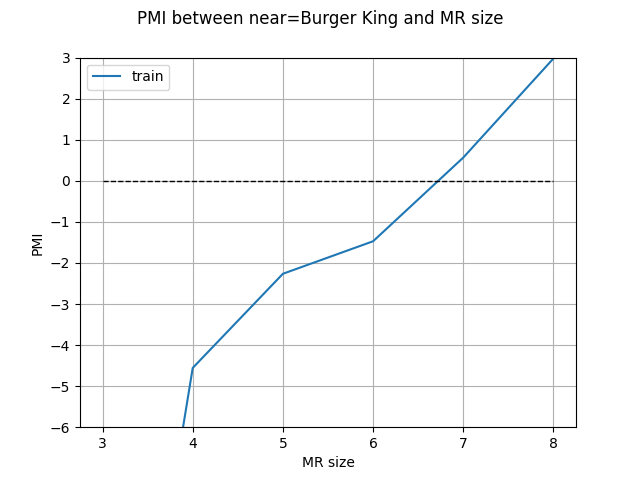
\includegraphics[scale=0.5]{nlg/nearbk.png}
\caption{PMI between \AV{near}{Burger King}~and \meaningrepresentation~size
on the E2E Challenge dataset. 0 on the $y$-axis indicates the two variables are independent.}
\label{fig:bkpmi}
\end{figure}


To demonstrate this, we trained a uni-directional GRU generation model on the training corpus
and then tried to generate an utterance for the following \meaningrepresentation,
\begin{center}
    \MR{\textsc{Inform}}
        {\AV{name}{Alimentum}}  
        {\AV{near}{Burger King}}
        {\AV{area}{city centre}}
        {\AV{family\_friendly}{no}}\end{center}
using beam search. Notice that in this case $\setsize{\mr}=4$,
indicating that the occurrence of \AV{near}{Burger King} is a 
relatively novel situtation given
 the training set.
We generated some beam search canditates we we show below, {\color{red}\uline{underlining in red}} the phrases that
are not semantically correct given the \meaningrepresentation,

\begin{enumerate}
\item Alimentum is located in the city centre {\color{red}\uline{near the Express by Holiday Inn.}} It is not family-friendly.     
\item Alimentum is located in the city centre {\color{red}\uline{near the Yippee Noodle Bar.}} It is not family-friendly.
\item Alimentum is located in the city centre {\color{red}\uline{near the Raja Indian Cuisine.}} It is not family-friendly.
\item Alimentum is not family-friendly. It is located in the city centre {\color{red}\uline{near the Yippee Noodle Bar.}}
\item The Alimentum is located in the city centre {\color{red}\uline{near the Express by Holiday Inn.}} It is not family-friendly.
%Alimentum is not family-friendly. It is located in the city centre near the Raja Indian Cuisine.\\\vspace{-1em}\\
%Alimentum is located in the city centre near the Clare Hall. It is not family-friendly.\\\vspace{-1em}\\
%Alimentum is located in the city centre near the crowne plaza hotel. It is not family-friendly.\\\vspace{-1em}\\
%Alimentum is not family-friendly. It is located in the city centre near the express by holiday inn.\\\vspace{-1em}\\
%The Alimentum is located in the city centre near the Yippee Noodle Bar. It is not family-friendly.\\\vspace{-1em}\\
%Alimentum is not family-friendly. It is located in the city centre near the Clare Hall.\\\vspace{-1em}\\
%The Alimentum is located in the city centre near the Raja Indian Cuisine. It is not family-friendly.\\\vspace{-1em}\\
%In the city centre near the express by holiday inn is Alimentum. It is not family-friendly.\\\vspace{-1em}\\
%Alimentum is located in the city centre near the city centre. It is not family-friendly.\\\vspace{-1em}\\
%Alimentum is located in the city centre near the rice boat. It is not family-friendly.\\\vspace{-1em}\\
%The Alimentum is not family-friendly. It is located in the city centre near the Yippee Noodle Bar.\\\vspace{-1em}\\
%Alimentum is located in the city centre near the rainbow vegetarian café. It is not family-friendly.\\\vspace{-1em}\\
%In the city centre near the Yippee Noodle Bar is the Alimentum. It is not family-friendly.\\\vspace{-1em}\\
%In the city centre near the Yippee Noodle Bar is Alimentum. It is not family-friendly.\\\vspace{-1em}\\
%
\end{enumerate}
Right away we are confronted by their homogeneity; utterances 1,2,3 and 5
have the same syntactic structure, varying only in the phrase \textit{near x}.
Utterances 1 and 5 differ only by a single word (the initial article \textit{The} in 5).  Most importantly, none of them correctly specify that the Alimentum 
is near Burger King. Even with a beam size of 128, the phrase \textit{Burger King} is never generated by the model!\footnote{A beam size of 128 would be impractial for most applications. Beam sizes are typically from 4-10 in most works.}


\begin{figure}[p]
\centering
    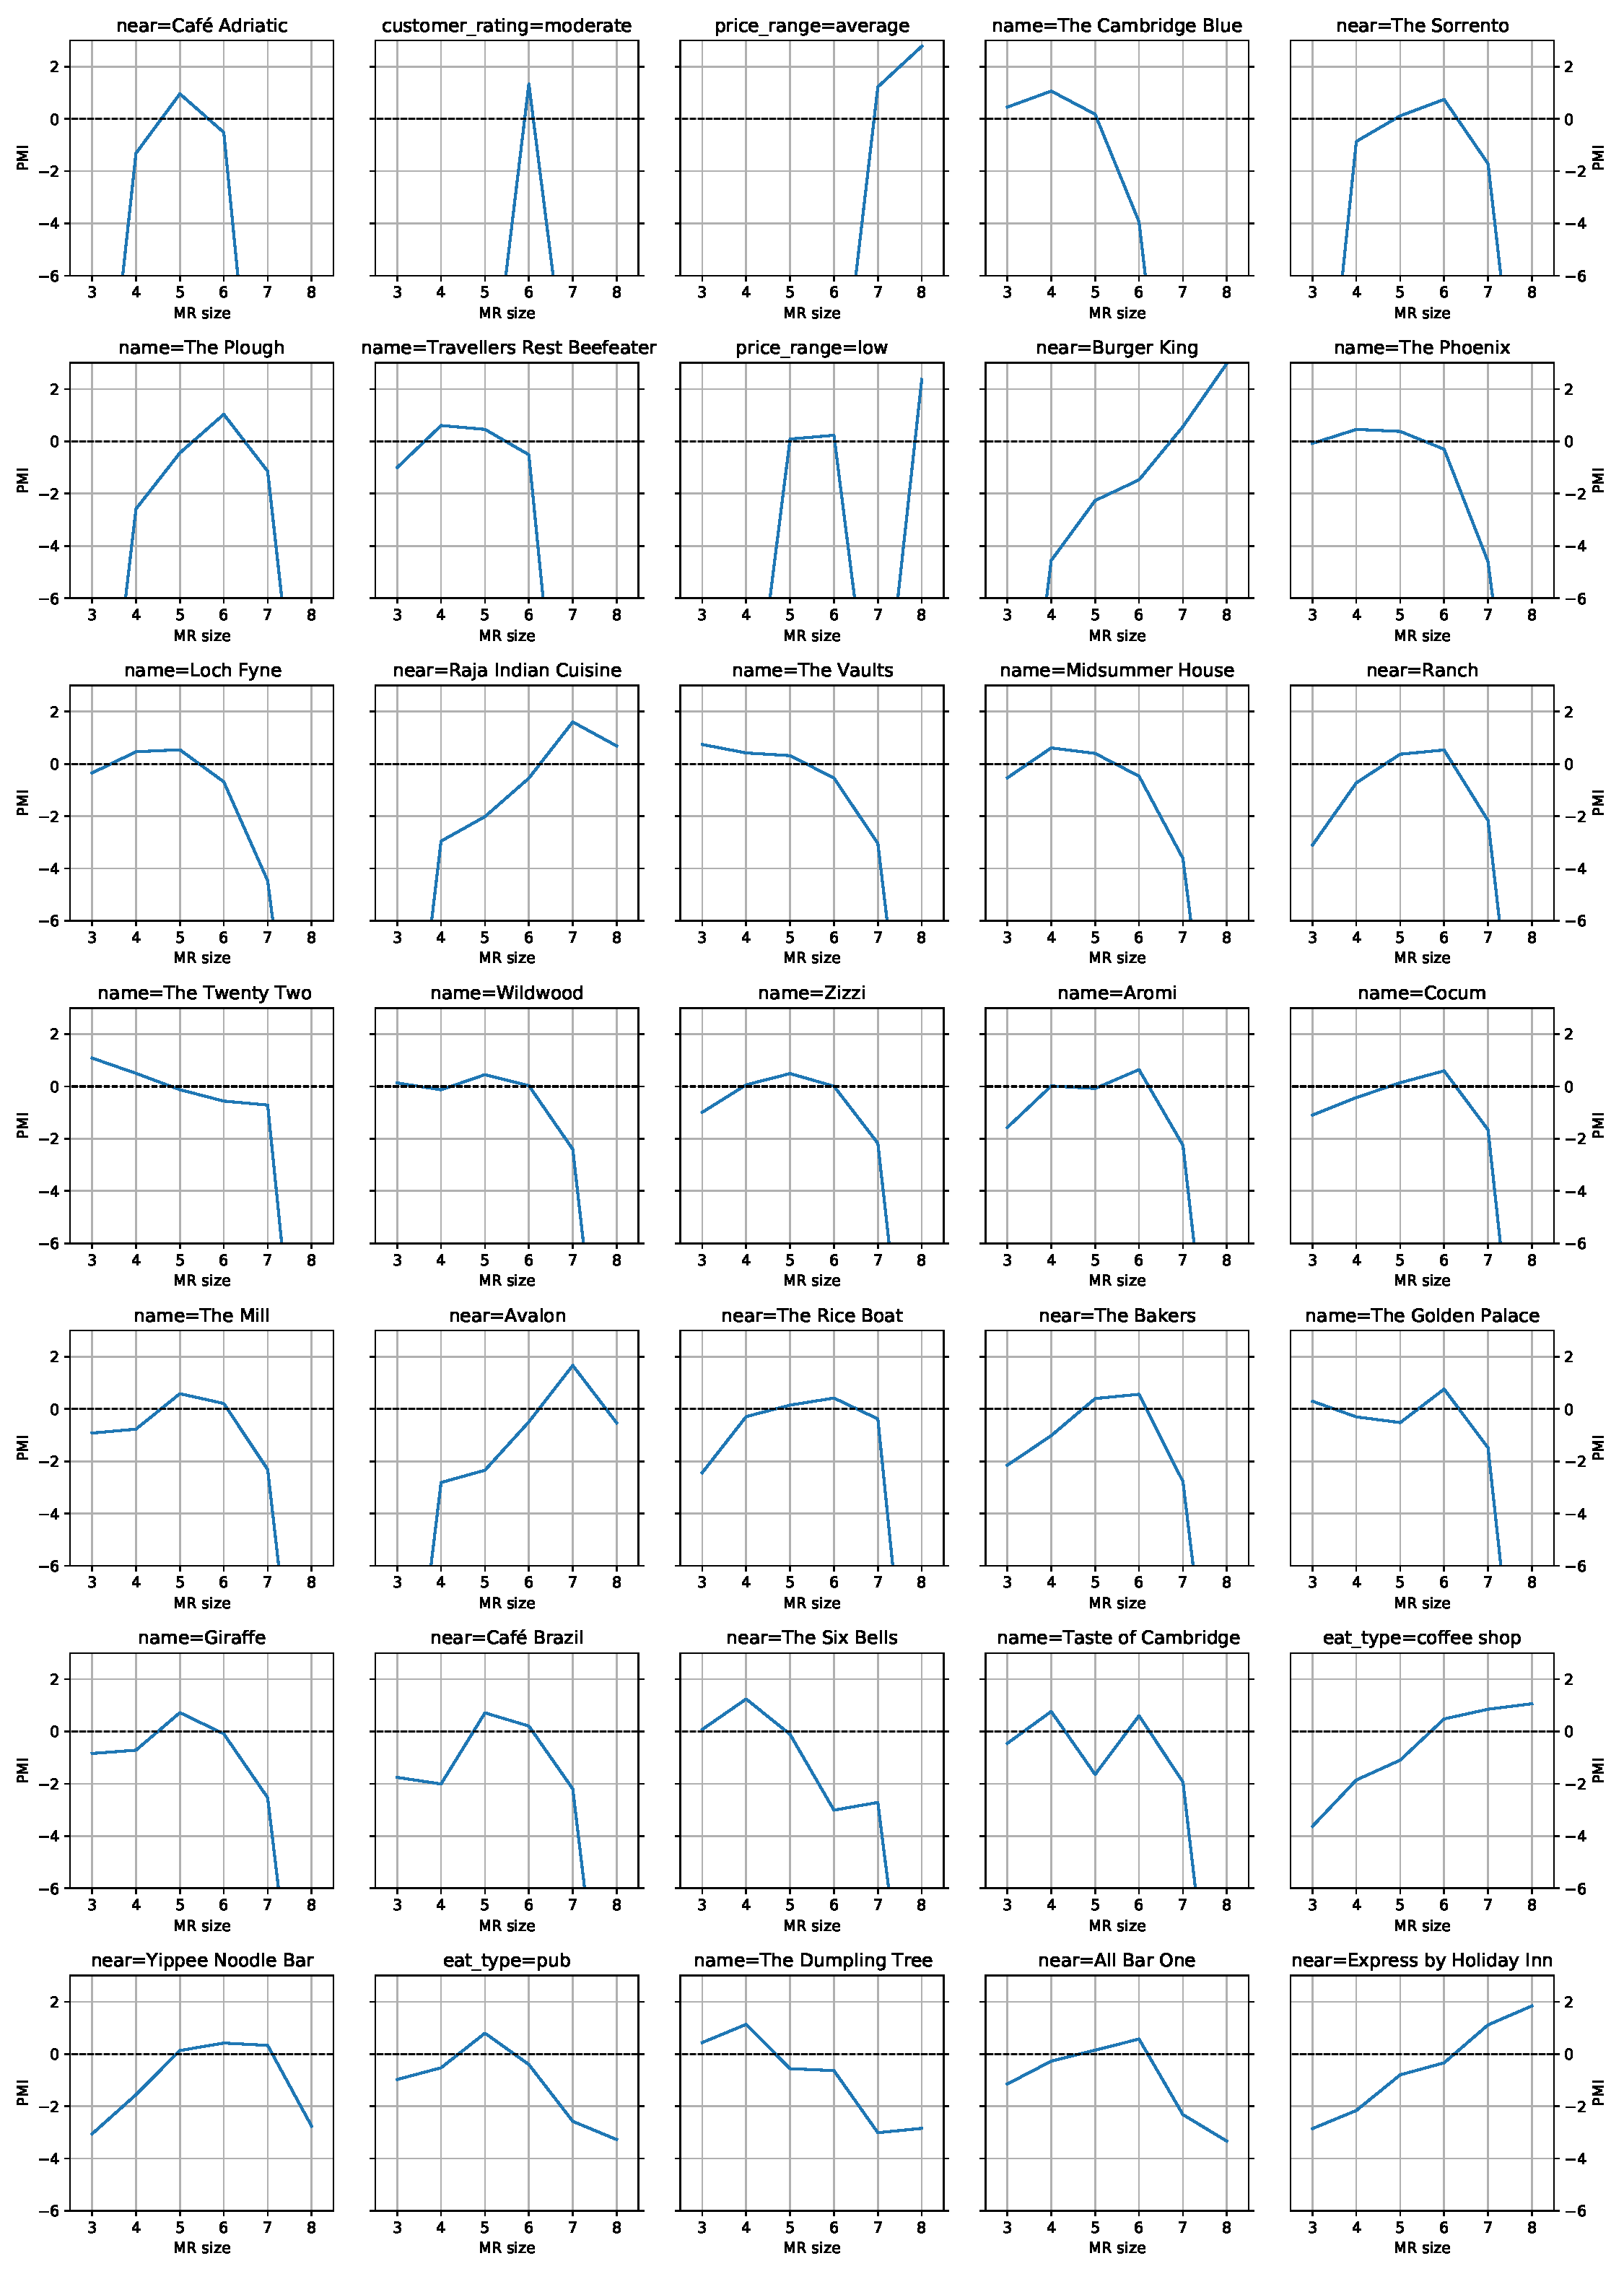
\includegraphics[width=0.9\textwidth]{nlg/trainpmis.pdf}
\caption{PMI between various \attributevalue s and \meaningrepresentation~size
on the E2E Challenge dataset. 0 on the $y$-axis indicates the two variables are independent.}
\label{fig:trainpmi}
\end{figure}


This is more frustrating because there are plenty of training examples where
even a coarse understanding of phrase structure would allow construction
of a correct utterance for this case.
For instance, we observe utterances containing \textit{near Burger King}
like this,
\begin{quotation}
\noindent \textit{The Eagle is a low rated coffee shop \textbf{near Burger King}
and the riverside that is family friendly and is less than £20
for Japanese food.}
\end{quotation}
while also seeing
\begin{quotation}
\noindent \textit{Alimentum is located in the city centre \textbf{near Yippee Noodle Bar}. \textellipsis}
% It serves expensive Italian food. It has an average customer rating.
\end{quotation}
where a correct utterance could be created by substituting ``Burger King''
in the latter instance, e.g., 
\begin{quotation}
\noindent \textit{Alimentum is located in the city centre \textbf{near Burge King}.}
% It serves expensive Italian food. It has an average customer rating.
\end{quotation}

Unfortunately, the GRU model does not learn to substitute the correct 
prepositional phrase. Given that correct examples seem constructable from
constituent phrases, it suggests that a data-augmentation approach
might help to generate additional training examples that do not possess 
some of the spurious correlations between \attributevalue s and input size.

Indeed, the compositional data-augmentation scheme proposed by \citet{andreas2020} demonstrates  improved model systematicity.
Unfortunately, a rule based system of recombination risks creating 
disfluencies in the utterances that could potentially reduce the fluency
of the learned model. Additionally, the number of spurious
associations in the dataset are numerous; see \autoref{fig:trainpmi} for 35 of the
total {\color{red}???} \attributevalue~pairs for the E2E dataset. They all have some 
spurious association with \meaningrepresentation~size. And we haven't even
explored other associations that might exist (e.g. between two \attributevalue~pairs). In the following subsections, we explore what an ideal
 data-augmentation policy might look like and then give a practical 
implementation of it.



%?This suggests that a data-augmentation strategy,
%?perhaps we can perform some recombination
%?of various trainging phrases and fragments, e.g. construct the example
%?This kind of data-augmentation has been helpful in making 
%?models behave more systematically \citep{thethinsg.}. 


%\clearpage


\subsection{An Idealized Data-Augmentation Protocol}
\label{sec:ideal}

We now introduce an idealized data-augmentation protocol and discuss some
potential pitfalls and bottlenecks before proposing our implementation 
of it.
Let $\corpus_\mrspace$ and $\corpus_\outSpace$
be the empirical distributions (i.e. training dataset distributions) over the \meaningrepresentations~and utterances
respectively. The emipirical distributions exhibit various dataset creation/annottation
artifacts. For example, we have that some attributes  are correlated
with length (i.e., $\corpus_\mrspace(a \in \mr, \setsize{\mr} = k) \ne 
\corpus_\mrspace(a \in \mr)\corpus_\mrspace(\setsize{\mr} = k)$) or 
certain attributes with each other
(i.e., $\corpus_\mrspace(a_1, a_2 \in \mr) \ne 
\corpus_\mrspace(a_1 \in \mr)\corpus_\mrspace(a_2\in \mr)$).



Ideally, we could construct novel \meaningrepresentation~examples such that
their distributions did not display these correlations. Let us assume we
have such a distrubtion, $\daMrDist$, from which we can sample novel
utterances. Given a sample $\samplmr \sim \daMrDist$, we would then need
a conditional distribution $\daUttDist(\samplmr)$ from which to 
draw the appropriate companion utterance $\samutttoks$ such that $\denotes{\samutttoks} = \samplmr$ while the naturalness/grammaticality of $\samutttoks$
was consistent with the empirical distribution, i.e. $\daUttDist \approx \corpus_\outSpace$. Having these two distributions, we could follow the
simple data-augmentation protocol in \autoref{alg:idealda} to obtain
a more systematic language generation model $\gen_*$.



Coming up with a 
\meaningrepresentation~distribution, $\daMrDist$, is fairly straightforward.
For example we could just sample the size of the \meaningrepresentation, $k$,
uniformly at random, then sample the $k$ \attributes~uniformly at random 
without replacement. This would ensure that attributes and \meaningrepresentation~size are independent and ensure that \attributes~are not correlated with
each other. To make up for the fact that some \attributevalues~are over-represented in the training set, we could sample values inversely proportional
to their empirical frequency. This results in the following data generation
process for 
\begin{singlespace}\[
\tilde{\mr}  = \left[\!\!\left[ 
\begin{array}{c} 
\delta~~~~~~~ \\
\AV{$a_1$}{$v_1$} \\ \vdots \\ \AV{$a_k$}{$v_k$}  
\end{array}  
\right]\!\!\right] \sim \daMrDist,\]\end{singlespace}
% Then for each of the attributes, values could be
%sampled inversely proportional to their occurrence in the training data, i.e.
{
\begin{minipage}{0.9\textwidth}
\begin{singlespace}
\noindent \textit{(1) Draw a dialogue act.}
\[
  \delta \sim \operatorname{Uniform}(\left\{\delta_1, \delta_2,\ldots\right\}) 
\]
\noindent \textit{(2) Draw a \meaningrepresentation~size $k$.}
\[
  k \sim \operatorname{Uniform}(\{k_{min}, \ldots, k_{max}\}) 
\]
\noindent \textit{(3) Sample $k$ attributes without replacement.}
\[
a_i  \sim \operatorname{Uniform}(\{name, \ldots, near, eat\_type\}\setminus\{a_1,\ldots,a_{i-1}\}) \quad \forall i: i \in  \{1,\ldots, k\}\]
\noindent \textit{(4) Sample a value $v_i$ for each attribute $a_i$.}
\[ v_i  \sim \operatorname{Categorical}\left(\operatorname{count}(v_1)^{-1}, \operatorname{count}(v_2)^{-1},\ldots\right)  \quad \forall i: i \in \{1,\ldots,k\}. \]
\end{singlespace}
\end{minipage}}
%\begin{align*}
%\operatorname{count}(a, v) & = \sum_{(\mr, \utttoks) \in \corpus} \mathds{1}\{\AV{$a$}{$v$} \in \mr  \}\\
%p(v|a) & = \frac{\operatorname{count}(a,v)^{-1}}{\sum_{v^\prime \in {\mrvocab}_a}  \operatorname{count}(a,v^\prime)^{-1}} \\
%a_i & \sim \operatorname{Uniform}(\{name, \ldots, near, eat\_type\}\setminus\{a_1,\ldots,a_{i-1}\}) & \forall i: i \in  \{1,\ldots, k\}\\
%v_i & \sim p(\cdot|a) & \forall i: i \in \{1,\ldots,k\} \\
%\tilde{\mr} & = \left[\!\!\left[ 
%\begin{array}{c} 
%\textsc{Inform} \\
%\AV{$a_1$}{$v_1$} \\ \vdots \\ \AV{$a_k$}{$v_k$}  
%\end{array}  
%\right]\!\!\right]
%\end{align*}\end{singlespace}
%This procedure should produce valid \meaningrepresentations, and by 
%definition $\daMrDist \ne \corpus_\mr$. Additionally, the co-occurance
%of an \attribute~and a particular \meaningrepresentation~size will now be 
%independent, and the co-occurrance of pairs of attributes will also be independent. 
%





\begin{algorithm}[t]
$\augdata \gets \{\}$\\
\While{$\setsize{\augdata} < \numSamples$}{
$\tilde{\mr} \sim \daMrDist$ \\
$\boldsymbol{\tilde{\utttoks}} \sim \daUttDist(\boldsymbol{\tilde{\mr}})$\\
%\If{ $\lnot \filter(\tilde{\mr}, \boldsymbol{\tilde{\utttoks}})$}{ $\augdata \gets \augdata \cup \{(\tilde{\mr}, \boldsymbol{\tilde{\utttoks}}) \}$ }
$\augdata \gets \augdata \cup \{(\tilde{\mr}, \boldsymbol{\tilde{\utttoks}}) \}$
}
%    \KwResult{Salience judgements $\bsals = \left[ \bsal_1, \ldots, \bsal_\docSize\right]$}
$\gen_* \gets \operatorname{Train}(\corpus \cup \augdata)$\\
\KwResult{$\gen_*$}
    \caption{Idealized Data-Augmentation and Training}
\label{alg:idealda}
\end{algorithm}

%If the novel \meaningrepresentations~are drawn from a distribution, 
%$\daMrDist$, such that $\daMrDist \ne \corpus_\mr$, 
%and the novel utterances are generated from $\daUttDist(\tilde{\mr})$
% such that $\denotes{\boldsymbol{\tilde{\utttoks}}} = \tilde{\mr}$
%while maintaining their fluency/naturalness (i.e., $\daUttDist \approx \corpus_\utttoks$),
%then 
%it is possible that that when training a \sequencetosequence~on the union 
%of original training data and synthetic data, the resulting model, $\gen_*$,
% will behave
%more systematically, which means more faithfully in our context.

Unfortunately, it is not clear how we implement utterance distribution
$\daUttDist(\samplmr)$ since if we had an utterance generation method that could
respond systematically to non-training data distributed \meaningrepresentations, we wouldn't need to perform data augmentation in the first place. As a starting point, 
we consider ways of generating samples from a base model $\gen_0$ which 
trained on the available training data, i.e. $\gen_0 = \operatorname{Train}(\corpus)$.




\subsection{Conditional Utterance Sampling for Data-Augmentation}

We cannot use $\gen_0$ with beam search as we saw previously,
there are some \meaningrepresentations~that $\gen_0$ won't be able to create utterances for (as we saw with \AV{near}{Burger King}). We could try a variant
of ancestral sampling, however 
it is difficult for ancestral sampling schemes to produce 
extremely different outputs that break from spurious associations learned
from the training distribution without hurting fluency. 



The fundamental issue with ancestral sampling is that the randomness of the
model at the word selection stage. This means that in the middle of generating
a phrase it is possible for a disfluent word to be selected, which can
disrupt the current phrase but also destabilize subsequent generation steps
as the model tries to recover from the unsual selection.
Ideally, randomness in a model would occur earlier in determining the 
``topicality'' or ``aboutness'' (you might even say content selection) 
of the generated utterance. 

Beyond the conditioning input $\ls(\mr)$,
the content that is to be generated is implicitly represented by
inner hidden states of the model. 
In \citet{cho2016}, they argue that the hidden states, $\decHidState_i$, 
of the \sequencetosequence~decoder lie on a manifold, as a requirement of
learning the next word prediction, i.e.
$\hat{\utttok} = \argmax_\utttok \gen(\utttok|\utttoks_{1:i},\ls(\mr)) = 
\argmax_\utttok \left(\weight{o}  \decHidState_i + \bias{o}\right)_\utttok$ 
implies that $\hat{\utttok}$ must be linearly separable from other 
words $\utttok^\prime \in \uttvocab$ along the hidden state manifold. The implication is that moving about the manifold will change 
the ``topicality'' of the distribution $\gen(\utttok|\utttoks_{1:i},\ls(\mr))$.
They further suggest adding Gaussian noise to $\decHidState_i$ as a way to
obtain random samples from $\gen$, which we refer to as noise-injection
sampling.

\newtcbox{\stochbox}[1][]{colframe=blue, colback=blue!15, boxrule=0.1mm,
                       nobeforeafter, tcbox raise base, shrink tight, extrude
                       by=0.32mm, #1}
\newtcbox{\detbox}[1][]{colframe=red, colback=red!15, boxrule=0.1mm,
                       nobeforeafter, tcbox raise base, shrink tight, extrude
                       by=0.32mm, #1}


\renewcommand{\algorithmcfname}{Alg.}

\begin{figure}[t]
\begin{center}\small \detbox{Deterministic operation}~~~~\stochbox{Stochastic operation}\end{center}
\resizebox{\textwidth}{!}{%
\begin{minipage}{0.33\textwidth}
\small
\begin{singlespace}
\begin{algorithm}[H]
$\encHidState_{1:\mrSize} \gets \operatorname{enc}(\ls(\mr))$\\
$\predutttok_1 \gets \starttok$\\
$\predutttoks \gets \left[ \predutttok_1\right]$\\
$i \gets 1$\\
\While{$\predutttok_i \ne \stoptok$}{
$\decHidState_i \gets \operatorname{dec}(\predutttoks, \encHidState_{1:\mrSize})$\\
$\vphantom{\boldsymbol{\epsilon_i} \sim \operatorname{Normal}(\zeroEmb, \frac{\sigma}{i})}$\\
\detbox{$\predutttok_{i+1} \gets \argmax_\utttok \gen(\utttok|\decHidState_i)$}\\
$\predutttoks \gets \predutttoks \oplus \left[ \predutttok_{i+1}\right]$\\
$i \gets i + 1$\\
}
%$\gen_* \gets \operatorname{Train}(\corpus \cup \augdata)$\\
\KwResult{$\predutttoks$}
    \caption{\small Greedy Decoding}
%\label{alg:idealda}
\end{algorithm}
\end{singlespace}
\end{minipage}\begin{minipage}{0.33\textwidth}
\small
\begin{singlespace}
\begin{algorithm}[H]
$\encHidState_{1:\mrSize} \gets \operatorname{enc}(\ls(\mr))$\\
$\predutttok_1 \gets \starttok$\\
$\predutttoks \gets \left[ \predutttok_1\right]$\\
$i \gets 1$\\
\While{$\predutttok_i \ne \stoptok$}{
$\decHidState_i \gets \operatorname{dec}(\predutttoks, \encHidState_{1:\mrSize})$\\
$\vphantom{\boldsymbol{\epsilon_i} \sim \operatorname{Normal}(\zeroEmb, \frac{\sigma}{i})}$\\
\stochbox{$\predutttok_{i+1} \sim \vphantom{\argmax_\utttok}\gen(\cdot|\decHidState_i)$}\\
$\predutttoks \gets \predutttoks \oplus \left[ \predutttok_{i+1}\right]$\\
$i \gets i + 1$\\
}
%$\gen_* \gets \operatorname{Train}(\corpus \cup \augdata)$\\
\KwResult{$\predutttoks$}
\caption{\small Ancestral Sampling}
%\label{alg:idealda}
\end{algorithm}
\end{singlespace}
\end{minipage}\begin{minipage}{0.38\textwidth}
\small
\begin{singlespace}
\begin{algorithm}[H]
$\encHidState_{1:\mrSize} \gets \operatorname{enc}(\ls(\mr))$\\
$\predutttok_1 \gets \starttok$\\
$\predutttoks \gets \left[ \predutttok_1\right]$\\
$i \gets 1$\\
\While{$\predutttok_i \ne \stoptok$}{
$\decHidState_i \gets \operatorname{dec}(\predutttoks, \encHidState_{1:\mrSize})$\\
\stochbox{$\boldsymbol{\epsilon_i} \sim \operatorname{Normal}(\zeroEmb, \frac{\sigma}{i})$}\\
\detbox{$\predutttok_{i+1} \gets \argmax_\utttok \gen(\utttok|\decHidState_i + \boldsymbol{\epsilon_i})$}\\
$\predutttoks \gets \predutttoks \oplus \left[ \predutttok_{i+1}\right]$\\
$i \gets i + 1$\\
}
%$\gen_* \gets \operatorname{Train}(\corpus \cup \augdata)$\\
\KwResult{$\predutttoks$}
\caption{\small Noise Injection Sampling}
%\label{alg:idealda}
\end{algorithm}
\end{singlespace}
\end{minipage}
}
\caption{A comparison of greedy decoding, ancestral sampling, and noise injection sampling.}
\label{fig:noiseinj}

%?\begin{minipage}{0.3\textwidth}
%?\begin{singlespace}
%?\begin{algorithm}[H]
%?$\predutttok_1 \gets \starttok$\\
%?$i \gets 1$\\
%?\While{$\predutttok_i \ne \stoptok$}{
%?$\tilde{\mr} \sim \daMrDist$ \\
%?%\If{ $\lnot \filter(\tilde{\mr}, \boldsymbol{\tilde{\utttoks}})$}{ $\augdata \gets \augdata \cup \{(\tilde{\mr}, \boldsymbol{\tilde{\utttoks}}) \}$ }
%?$\augdata \gets \augdata \cup \{(\tilde{\mr}, \boldsymbol{\tilde{\utttoks}}) \}$
%?}
%?%    \KwResult{Salience judgements $\bsals = \left[ \bsal_1, \ldots, \bsal_\docSize\right]$}
%?$\gen_* \gets \operatorname{Train}(\corpus \cup \augdata)$\\
%?\KwResult{$\gen_*$}
%?    \caption{Noise-Injection Sampling}
%?\label{alg:idealda}
%?\end{algorithm}
%?\end{singlespace}
%?\end{minipage}
\end{figure}





We show the noise-injection sampling algorithm in \autoref{fig:noiseinj}
along with greedy decoding and ancestral sampling to emphasize the 
how the location of the stochasticity moves from the next word selection (line 8) to a peturbation of the hidden state (line 7). 
Note that in line 7 of the noise injection sampling algorithm, the standard
deviation of the normal distribution, $\frac{\sigma}{i}$, is scaled by the 
decoder step $i$ and in the limit turns to zero, i.e. $\lim_{i \rightarrow +\infty} \decHidState + \boldsymbol{\epsilon}_i = \decHidState$. The inuition 
behind this scaling is that we add the most noise at the first steps 
of decoding, which encourages the decoder to start from a topically novel
region of the hidden state manifold. As the decoding proceeds, the noise
reduces along with the chances of sending the decoder off the manifold
and destabilizing the decoding, and gradually we converge on the behavior of
greedy decoding. 


We can understand noise-injection sampling as a compromise between
greedy decoding and ancestral sampling; rather than draw a sequence of utterance
tokens stochasticity, we instead draw a sequence of hidden state spaces.
Given the sequence of hidden state spaces, the corresponding sequence of
utterance tokens is deterministically decided by the most likely next token
given the last hidden state. This next word selection strategy helps to
avoid disfluent continuations.


\begin{figure}[t]
\small
\textbf{Ancestral Sampling}\\
\textit{\starttok~the eagle is a non family - friendly italian food establishment . \stoptok}\\
\textit{\starttok~the eagle is a italian food place and is not family - friendly . \stoptok}\\
\textit{\starttok~some italian food can be found at the eagle . \senttok~it 's not family - friendly . \stoptok}\\
\textit{\starttok~the eagle serves italian food . \senttok~it has a \unktok~\unktok~and is not family friendly . \stoptok}\\
\textit{\starttok~the eagle is a family friendly place for italian food . \stoptok}\\
~\\
\textbf{Top-K Sampling ($k=100$)}\\
\textit{\starttok~the eagle serves italian food . \senttok~it is not family - friendly . \stoptok}\\
\textit{\starttok~the eagle serves italian cuisine . \senttok~it is not family - friendly . \stoptok}\\
\textit{\starttok~the eagle has italian food and is not family - friendly \stoptok}\\
\textit{\starttok~the eagle is italian place . \senttok~it is not family - friendly . \stoptok}\\
\textit{\starttok~the eagle provides fast food . \senttok~it is not family - friendly . \stoptok}\\
~\\
\textbf{Nucleus Sampling ($p=0.95$)}\\
\textit{\starttok~the eagle serves italian food and is not family - friendly . \stoptok}\\
\textit{\starttok~the eagle is not family - friendly and serves italian food . \stoptok}\\
\textit{\starttok~the eagle is not family - friendly . \senttok~they serve italian food . \stoptok}\\
\textit{\starttok~italian food is served at the eagle . \senttok~not family - friendly . \stoptok}\\
\textit{\starttok~the eagle is a good place to eat italian food . \senttok~it is not family - friendly . \stoptok}\\
~\\
\textbf{Noise-Injection Sampling ($\sigma=2.0$)}\\
\textit{\starttok~the eagle in the city centre . \senttok~it is not family - friendly . \senttok~it is located near the burger king . \stoptok}\\
\textit{\starttok~the eagle serves italian food . \stoptok}\\
\textit{\starttok~the waterman is not family friendly and is located near burger king . \stoptok}\\
\textit{\starttok~the eagle is located near the burger king . \stoptok}\\
\textit{\starttok~the eagle is a non family - friendly italian food place . \stoptok}\\
\caption{Example samples taken after conditioning on the following  meaning representation: 
$\left[\!\!\left[\textsc{Inform};\quad    \AV{name}{The Eagle};\quad \AV{food}{Italian};\quad \AV{family\_friendly}{yes}\right]\!\!\right]$. }
\label{fig:examplesamples}
\end{figure}


In \autoref{fig:examplesamples} we show examples of samples obtained with
noise-injection sampling as well as some ancestral sampling schemes.
We can see that the ancestral sampling examples are not very diverse.
The noise-injection sampling
example, however, semantically diverges from the input while maintaining
fluency. It was even able to generate an utterance containing the phrase
``near Burger King'' which is was practically impossible to generate with
beam search.


\begin{table}
    \centering
    \begin{tabular}{c ccc ccc ccc ccc ccc}
        \toprule
        $i$ & 1 & 2 & 3 & 4 &5 & 6 \\
        $\utttok_{i+1}$ &  the  & waterman &is &not& family & friendly \\
        \midrule
        $\gen(\utttok_{i+1}|\decHidState_i; \topkVocab{5}{i})$ & 0.874 & 0.004 & 0.380 & 0.397 & 0.915 & 0.147 \\
    $\gen(\utttok_{i+1}|\decHidState_i; \topkVocab{25}{i})$ &
0.792 & 0.004 & 0.344 & 0.371 & 0.877 & 0.147 \\
     $\gen(\utttok_{i+1}|\decHidState_i; \topkVocab{50}{i})$ &
0.778 & 0.004 & 0.339 & 0.366 & 0.872 & 0.147 \\
       $\gen(\utttok_{i+1}|\decHidState_i; \topkVocab{75}{i})$ &
0.772 & 0.004 & 0.338 & 0.364 & 0.870 & 0.147 \\
        $\gen(\utttok_{i+1}|\decHidState_i; \topkVocab{100}{i})$ & 
0.768 & 0.004 & 0.337 & 0.363 & 0.869 & 0.147 \\
        \midrule
     $\gen(\utttok_{i+1}|\decHidState_i; \nucleusVocab{.95}{i})$     & 
0.796 & 0.000 & 0.352 & 0.377 & 0.909 & 0.148 \\
     $\gen(\utttok_{i+1}|\decHidState_i; \nucleusVocab{.96}{i})$ &
0.789 & 0.000 & 0.349 & 0.374 & 0.898 & 0.148 \\
      $\gen(\utttok_{i+1}|\decHidState_i; \nucleusVocab{.97}{i})$ &
0.781 & 0.000 & 0.345 & 0.370 & 0.892 & 0.148 \\
     $\gen(\utttok_{i+1}|\decHidState_i; \nucleusVocab{.98}{i})$ &
0.773 & 0.000 & 0.342 & 0.367 & 0.882 & 0.148 \\ 
     $\gen(\utttok_{i+1}|\decHidState_i; \nucleusVocab{.99}{i})$ &
0.765 & 0.004 & 0.338 & 0.363 & 0.874 & 0.148 \\
        \midrule
        $\gen(\utttok_{i+1}|\decHidState_i)$ &0.758 & 0.004 & 0.335 & 0.359 & 0.865 & 0.147 \\
        $\gen(\utttok_{i+1}|\decHidState_i + \boldsymbol{\epsilon}_i)$ & 0.321 & 0.170 & 0.408 & 0.489 & 0.785 & 0.514 \\
        \bottomrule
    \end{tabular}

~\\~\\~\\~\\


    \begin{tabular}{c ccc ccc ccc ccc ccc}
        \toprule
        $i$             & 7  & 8 & 9 & 10 & 11 & 12 & 13 & 14 \\
        $\utttok_{i+1}$ &  and &is& located &near& burger & king & . & \stoptok \\
        \midrule
 $\gen(\utttok_{i+1}|\decHidState_i; \topkVocab{5}{i})$ &  0.338 & 0.111 & 0.147 & 0.168 & 0.000 & 0.954 & 0.931 & 0.810 \\
 $\gen(\utttok_{i+1}|\decHidState_i; \topkVocab{25}{i})$ & 0.327 & 0.101 & 0.111 & 0.148 & 0.001 & 0.935 & 0.911 & 0.810 \\
 $\gen(\utttok_{i+1}|\decHidState_i; \topkVocab{50}{i})$ & 0.326 & 0.100 & 0.105 & 0.146 & 0.001 & 0.930 & 0.910 & 0.810 \\
 $\gen(\utttok_{i+1}|\decHidState_i; \topkVocab{75}{i})$    & 0.326 & 0.100 & 0.103 & 0.145 & 0.001 & 0.928 & 0.909 & 0.810 \\
 $\gen(\utttok_{i+1}|\decHidState_i; \topkVocab{100}{i})$ & 0.326 & 0.100 & 0.102 & 0.144 & 0.001 & 0.926 & 0.909 & 0.810 \\
        \midrule
   $\gen(\utttok_{i+1}|\decHidState_i; \nucleusVocab{.95}{i})$      & 0.342 & 0.104 & 0.103 & 0.150 & 0.000 & 0.964 & 0.950 & 0.810 \\
   $\gen(\utttok_{i+1}|\decHidState_i; \nucleusVocab{.96}{i})$ & 0.338 & 0.103 & 0.102 & 0.149 & 0.000 & 0.954 & 0.939 & 0.810 \\
$\gen(\utttok_{i+1}|\decHidState_i; \nucleusVocab{.97}{i})$
     & 0.333 & 0.102 & 0.101 & 0.148 & 0.000 & 0.947 & 0.931 & 0.810 \\
 $\gen(\utttok_{i+1}|\decHidState_i; \nucleusVocab{.98}{i})$   
     & 0.332 & 0.101 & 0.100 & 0.146 & 0.000 & 0.937 & 0.924 & 0.810 \\
 $\gen(\utttok_{i+1}|\decHidState_i; \nucleusVocab{.99}{i})$
     & 0.329 & 0.100 & 0.099 & 0.145 & 0.001 & 0.928 & 0.917 & 0.810 \\
 \midrule
        $\gen(\utttok_{i+1}|\decHidState_i)$ & 0.326 & 0.099 & 0.098 & 0.143 &0.001 & 0.919 & 0.908 & 0.810\\
        $\gen(\utttok_{i+1}|\decHidState_i + \boldsymbol{\epsilon}_i)$ & 0.459 & 0.562 & 0.440 & 0.731 &0.599 & 0.972 & 0.903 & 0.984 \\
 \bottomrule
    \end{tabular}

    \caption{Word selection probabilities when using ancestral sampling,
        top-$k$ sampling (for $k \in \{5,25,50,75,100\}$), 
    nucleus samplling (for $\nucleusthr \in \{0.95, 0.96, 0.97, 0.98, 0.99\}$), and noise-injection sampling ($\sigma = 2.0$).}
    \label{tab:sampprobs}
\end{table}




In \autoref{tab:sampprobs}, we show the probability of generating the 
example

\begin{center}
\textit{\starttok~the waterman is not family friendly and is located near burger king . \stoptok}\end{center}

\noindent under the various sampling schemes. In our present case, top-$k$ and nucleus
sampling have very similar distributions to the ancestral sampling
distribution ($\gen(\utttok_{i+1}|\decHidState_i)$). All three of these 
techniques assign a very low probability to generating the example utterance,
and in the case of nucleus sampling, it only gives non-zero probability when
using a nucleus of 0.99 cumulative probability (i.e. $\nucleusVocab{.99}{i}$)!
In particular, noise-injection sampling puts much more probability 
mass on generating relatively rare \attributevalue~realizations ($i=2$, ``waterman'' and $i=11$, ``burger''). This aspect of noise-injection sampling
makes it very attractive for data-augmentation as we can use it to create
semantically novel utterances that are not represented in the training dataset,
while still producing fluent outputs.




\subsection{A Practical Data-Augmentation Protocol}
\label{sec:daprotos}



\newtcbox{\truttbox}[1][]{colframe=green, colback=green!15, boxrule=0.1mm,
                       nobeforeafter, tcbox raise base, shrink tight, extrude
                       by=0.32mm, #1}
\newtcbox{\mrdistbox}[1][]{colframe=orange, colback=orange!15, boxrule=0.1mm,
                       nobeforeafter, tcbox raise base, shrink tight, extrude
                       by=0.32mm, #1}

\newtcbox{\ninjbox}[1][]{colframe=purple, colback=purple!15, boxrule=0.1mm,
                       nobeforeafter, tcbox raise base, shrink tight, extrude
                       by=0.32mm, #1}
\newtcbox{\correctbox}[1][]{colframe=blue, colback=blue!15, boxrule=0.1mm,
                       nobeforeafter, tcbox raise base, shrink tight, extrude
                       by=0.32mm, #1}
\newtcbox{\filterbox}[1][]{colframe=cyan, colback=cyan!15, boxrule=0.1mm,
                       nobeforeafter, tcbox raise base, shrink tight, extrude
                       by=0.32mm, #1}

\newtcbox{\returnbox}[1][]{colframe=violet, colback=violet!15, boxrule=0.1mm,
                       nobeforeafter, tcbox raise base, shrink tight, extrude
                       by=0.32mm, #1}

\begin{figure}[t]
\begin{singlespace}
\begin{algorithm}[H]
\truttbox{$\gen_0 \gets \operatorname{Train}_\utttoks\left(\corpus\right)$} \\
\truttbox{$\dmodel \gets \operatorname{Train}_\mr\left(\corpus\right)$} \\
$\augdata \gets \left\{ \right\}$\\
\While{$\setsize{\augdata} < \numSamples$}{
\mrdistbox{$\samplmr \sim \pdaMrDist$}\\
\ninjbox{$\pdaCandUtts\gets \left\{ \pdaCandUtt \sim 
            \gen_0\left(\cdot|\ls(\samplmr), \pdaCandEps\right) 
            \quad \forall i : i \in \{1,\ldots, k\} \right\} $}\label{lst:pdacand}\\
\ninjbox{$\predutttoks \gets
    \argmax_{\pdaCandUtt \in \pdaCandUtts} 
    \frac{\log \gen_0\left(\pdaCandUtt|\ls(\samplmr),\pdaCandEps \right)}{\setsize{\pdaCandUtt}}$}\label{lst:pdacandselect}\\
\correctbox{$\pdaPredMr \gets \dmodel\left(\predutttoks\right)$}\\
\If{\filterbox{$\lnot \operatorname{Filter}\left(\pdaPredMr, \predutttoks\right)$}}{
    $\augdata \gets \augdata \cup \left\{ \left(\pdaPredMr, \predutttoks\right) \right\}$
}
~\\
}
\returnbox{$\gen_1 \gets \operatorname{Train}_\utttoks(\corpus \cup \augdata)$}\\
\KwResult{$\gen_1$}
    \caption{Data Augmentation with Noise-Injection Sampling and Self-Training }
%\label{alg:idealda}
\end{algorithm}
\end{singlespace}
\caption{A comparison of greedy decoding, ancestral sampling, and noise injection sampling.}
\label{fig:practda}
\end{figure}


Because of its ability to generate semantically divergent and novel
outputs while maintaining fluency, we adopt this noise-injection
sampling as our method of sampling utterances, $\daUttDist$, for 
data-augmentation. We show our actual data-augmentation scheme in
\autoref{fig:practda} and now walk through some of the implementation details.

\paragraph{\truttbox{Train base generator $\gen_0$ and \meaningrepresentation~parser $\dmodel$.}}
The algorithm begins by training the base generator, i.e. na{\"i}ve 
\sequencetosequence~model, and \meaningrepresentation~parser $\dmodel$. 
Both models are trained on the same data, with the only real change to the 
$\operatorname{Train}$ sub-routine being which part of a training example
is the ouput and which is the input. Alternatively, $\dmodel$ can 
also be implemented using regular-expression-based rules. We defer detailed 
explanation of $\dmodel$ until the experiments; it suffices to understand
$\dmodel$ as a mapping from utterances to \meaningrepresentations.




\paragraph{\mrdistbox{Sampling a \meaningrepresentation, $\samplmr$}}
We use the meaning representation described in \autoref{sec:ideal} to implement
 the distribution $\corpus_\mr^{-1}$. 

\paragraph{\ninjbox{Generating a novel utterance with noise-injection 
    sampling.}}
    In \autoref{lst:pdacand} we take $200$ noise-injection samples to construct
    a candidate set of utterances, $\pdaCandUtts_{200}$. 
    From these we use only the top 20 utterances, $\pdaCandUtts_{20}$ by average log-likelihood,
    $\frac{\log\gen(\pdaCandUtt|\ls(\samplmr), \boldsymbol{\epsilon}^{(i)})}{\setsize{\pdaCandUtt}}$ (\autoref{lst:pdacandselect}).
%    From $\pdaCandUtts$ we
%    select as our noise-injection sample, the utterance $\predutttoks$
%    which has the highest average token log-likelihood (\autoref{lst:pdacandselect}). 
    We do this selection step so as to be extra cautious and avoid adding
    any potentially disfluent utterances to $\augdata$.
    
    \paragraph{\correctbox{Predict \meaningrepresentation~$\pdaPredMr$ from
    $\predutttoks$.}} Because the noise-injection sampling produces highly
semanticly divergent utterances, it is unlikely that $\denotes{\predutttoks } = \samplmr$. Instead we use the \meaningrepresentation~parser, $\dmodel$, to
recover the most likely \meaningrepresentation, $\pdaPredMr = \dmodel\left(\predutttoks\right)$.

\paragraph{\filterbox{Check synthetic datapoint $(\pdaPredMr,\predutttoks)$.}}
We do one last quality check on the synthetic example $(\pdaPredMr,\predutttoks)$ before adding it to the augmented dataset, $\augdata$. We make sure that
the probability of $\pdaPredMr$ under $\dmodel$ is above 0.5 when using
a model-based \meaningrepresentation~parser. When using a rule-based
\meaningrepresentation~parser, we check to make sure that there are no
repeated \attributevalue-pairs in $\predutttoks$, e.g., ``Aromi is a 
coffee shop and it is a coffee shop.'' Meaning representation/utterances that
have been previously generated are also discarded. If the \meaningrepresentation/utterance
pair passes these final quality checks, we add it to $\augdata$.

\paragraph{\returnbox{Train an augmented generator $\auggen$ on $\corpus \cup \augdata$.}} After generating a synthetic dataset, $\augdata$, we train a new 
generation model, $\auggen$, on the union of the original training data
and the newly generated synthetic data. We refer to this model as 
the augmented generator and, as we will show empirically, the augmented
generator is more faithful than the base generator, $\gen_0$.
We call this process self-training because $\auggen$ and $\gen_0$ share 
the same architecture, and $\auggen$ is trained on data produced by $\gen_0$.



\subsection{Datasets}

\begin{table}
\centering
\begin{tabular}{ccc ccc}
\toprule
Dataset & Train & Valid & Test & Unique Dialogue Acts & Unique Attribute Values \\
\midrule
E2E Chal. & 42,061 & 4672 & 4693 & 1 & 8 \\
Laptops & 15,888 & 5,298 & 5,297 & 14 & 19\\
TVs & 8,442 & 2,814 & 2,812 & 14 & 15\\
\bottomrule
\end{tabular}
\caption{Dataset statistics for noise-injection and self-training 
experiments.}
\label{tab:fgds}
\end{table}


We experimentally validate the noise-injection sampling and self-training
data-augmentation scheme on three recent dialgue generation datasets,
the E2E Challenge dataset~\citep{novikova2017} 
and the Laptops and TVs datasets \citep{wen2016}.
%three collections of 
%\meaningrepresentation/utterance pairs for training response generation models
%
%
%We use three recent dialogue generation datasets in our experiments,
%the E2E Challenge Dataset \cite{novikova2017}, and the Laptops and 
%TVs datasets \cite{wen2016}.
%We only briefly review them here.
Each dataset consists of \meaningrepresentations~paired with one or more 
reference utterances.
%(see \autoref{figure:introexample} for an example from the E2E dataset).
%The structure of each \meaningrepresentation~is relatively simple, 
%consisting of the 
%dialog act itself, (e.g. \textit{inform}, \textit{recommend}, 
%\textit{compare}, etc.) and a variable number of attribute slots
%which need to be realised in the utterance. 
All attribute values 
come from a closed vocabulary.
%If an attribute is not present in the MR it should not be realized in the 
%corresponding utterance. 

The three datasets also represent different training size conditions; 
with the E2E Challenge dataset representing the ``large data'' training
condition and the Laptops and TVs dataset representing ``small data'' conditinos. See \autoref{tab:fgds} for dataset size statistics.
The E2E Challenge dataset has only one dialogue act, \textsc{Inform}, 
and its training \meaningrepresentations~contain three to eight
\attributes~unique attributes. 
The Laptops and TVs datasets contain a more diverse set of \meaningrepresentation/utterance pairs. There are 14 unique dialogue acts. 
The number of minimum and maximum \attributes~varies according to the dialogue
act. See \autoref{tab:fgdas} for a list of the unique dialogue acts
and attributes for the three training sets. 

\begin{table}
\centering
\begin{tabular}{llll}
\toprule
Dataset & Dialog Acts & \multicolumn{2}{c}{Attributes} \\
\midrule
 \multirow{8}{*}{E2E Challenge} & \textsc{Inform} & name \\
 & & near \\
 & & eat\_type \\
 & & food \\
 & & area \\
 & & price\_range \\
 & & customer\_rating \\
 & & family\_friendly \\
\midrule
\multirow{14}{*}{Laptops} & \textsc{Inform} & family & weight\\
& \textsc{InformOnlyMatch} & price\_range & platform\\
& \textsc{InformOnMatch} & battery\_rating & memory\\
& \textsc{InformAll} & drive\_range & drive \\ 
& \textsc{InformCount} & weight\_range & processor \\
& \textsc{InformNoInfo} & is\_for\_business\_computing\\
& \textsc{Recommend} &name\\ 
& \textsc{Compare}& type \\
& \textsc{Select}& price\\
& \textsc{Suggest}& warranty\\
& \textsc{Confirm} & battery\\ 
& \textsc{Request}&design\\
& \textsc{RequestMore} &dimension \\
& \textsc{Goodbye} & utility\\
\midrule
 \multirow{14}{*}{TVs} & \textsc{Inform} & family & audio \\
& \textsc{InformOnlyMatch} & price\_range \\
& \textsc{InformOnMatch} & screen\_size\_range \\
& \textsc{InformAll} & eco-rating\\ 
& \textsc{InformCount}& hdmi-port\\
& \textsc{InformNoInfo}& has\_usb-port\\
& \textsc{Recommend} & name \\ 
& \textsc{Compare} & type \\
& \textsc{Select} &price\\
& \textsc{Suggest} & resolution\\
& \textsc{Confirm} & power\_consumption\\ 
& \textsc{Request} & accessories\\
& \textsc{RequestMore}& color \\
& \textsc{Goodbye} & screen\_size\\
\bottomrule
\end{tabular}
\caption{The dialogue acts and attributes for the E2E Challenge, Laptops, and TVs datasets.}
\label{tab:fgdas}
\end{table}



\paragraph{Delexicalization}
Prior work using neural \naturallanguagegeneration~models often relies on 
delexicalization, that is, replacing realizations of named-entity or 
numeric values in an utterance with a placeholder token, in order to alleviate
data sparsity issues and yield better generalization when a generating utterances about named-entities not seen in the training dataset. For example
on the E2E Challenge dataset, the \Atr{name}~and \Atr{near}~attributes
are often delexicalized because they are proper names of estabilishments
that are simple to find and replace in the utterance.
When delexicalizing the \Atr{name}~and \Atr{near}~attributes,
the fully lexicalized utterance 

\begin{center}\noindent~~~~\textit{Near The Six Bells is a venue that is children
friendly named The Golden Curry.}\end{center}

\noindent can be delexicalized as

\begin{center}\noindent ~~~~\textit{Near <<near>> is a venue that is children
friendly named <<name>>.}\end{center}

\noindent Delexicalized utterances can be re-lexicalized as a post-processing
step, where the placeholder token is replaced with the correct value text.

On the E2E Challenge dataset, we experiment with delexicalization of the 
\textit{Name} and \textit{Near} attributes since they have a relatively large vocabulary of valid slot fillers, some of which are only seen  infrequently in the training data;
it can be difficult for fully lexicalized models to produce some of the 
rarer location names for these attributes. 

However, since delexicalization might be difficult or 
impossible in other domains, we implement both delexicalized and lexicalized
versions of the generation models on the E2E dataset to 
more fully evaluate the
self-training method.
   

The evaluation script for the Laptops and TVs datasets uses delexicalization
to evaluate attribute realization error, and so we use it here to be 
consistent with prior work, 
delexicalizing all possible attributes.
%




\subsection{Text Generation Models}

We use a two-layer, unidirectional GRU architecture with Bahdanau style
attention for our 
 \sequencetosequence~\meaningrepresentation-to-text model. We set $\embDim = \hidDim = \encDim = \decDim = 512$, that is, we use 512-dimensional embedding and hidden states as 
described in \autoref{sec:nlggru}.
We fit model parameters, $\params$, by minimizing the negative log-likelihood
of the training set, $\corpus$, i.e. \[\mathcal{L}(\params) = - \sum_{(\mr, \utttoks) \in \corpus  }  \log \gen\left(\utttoks|\ls(\mr);\params\right).\]

Our choice of linearization strategy, $\ls$, differs slightly for the 
E2E Challenge and ViGGO corpora. For the former, we arbitrarily and 
consistently order the eight attribues, explicitly representing absent
\attributevalues~with a \textit{N/A} token. For example, for the \meaningrepresentation, 
\begin{singlespace}
    \centering
    \MR{\textsc{Inform}}{\AV{name}{The Mill}}{\AV{near}{Avalon}}{\AV{food}{Italian}}
\end{singlespace}
\noindent we would have the following linearization,
\[ \ls(\mr) = \left[\begin{array}{l} \starttok,\\ \textit{eat\_type=N/A},\\ \textit{near=Avalon},\\ \textit{area=N/A}, \\ \textit{family\_friendly=N/A},\\ \textit{customer\_rating=N/A}, \\\textit{price\_range=N/A},\\ \textit{food=Italian},\\ \textit{name=The Mill}\\ \stoptok \end{array}\right].\] 
    We omit the dialogue act since the E2E Challenge dataset only has one, \textsc{Inform}. When
    using the delexicalized model variant, we omit the name attribute since
    it is always present, and only indicate that the near attribute is present
    with a placeholder
    token, yielding 
\[ \ls(\mr) = \left[\begin{array}{l} \starttok,\\ \textit{eat\_type=N/A},\\ \textit{near=<<present>>},\\ \textit{area=N/A}, \\ \textit{family\_friendly=N/A},\\ \textit{customer\_rating=N/A}, \\\textit{price\_range=N/A},\\ \textit{food=Italian},\\ \stoptok \end{array}\right].\] 

    For the Laptops and TVs corpus, we similarly determine an arbitrary ordering
    but omit any absent attribute-values since there are too many to represent
    all of them explicitly. Additionally, since there are multiple dialogue acts we prepend a token representing the dialogue act to the start of the sequence. As an example, for the following \meaningrepresentation, \\[-15pt]
\begin{singlespace}
    \centering
    \MR{\textsc{InformCount}}{\AV{count}{40}}{\AV{family}{don't care}}{\AV{battery\_rating}{excellent}}
\end{singlespace}~\\
\noindent we would have the following linearization,
\[\ls(\mr) = \left[\starttok, \textit{inform\_count}, \textit{count=<<NUM>>}, \textit{family=don't care}, \textit{battery\_rating=excellent}, \stoptok\right].  \]



When generating utterances for evaluation (i.e. not for use in noise-injection sampling) we use either greedy decoding or beam decoding with a 
beam size of eight.
The beam search terminates after eight candidates have been generated;
the candidates are reranked by average token log-likelihood, $\frac{\log \gen\left(\utttoks|\ls(\mr)\right)}{\setsize{\utttoks}}$. In these experiments, we \textbf{do not} use a discriminative reranker to ensure the faithfulness of the 
selected beam candidate. 



\subsection{\MeaningRepresentation~Parsing Models}

Given a novel utterance $\predutttoks$~sampled from $\gen$, we need to 
reliably parse the implied \meaningrepresentation, i.e. 
$\pdaPredMr = \dmodel(\predutttoks)$, 
where $\dmodel$~is our parsing model. We have two things going for us in 
our experimental setting. First, even with noise-injection sampling,
model outputs are fairly patterned, reducing the variability of the utterances
we need to parse in practice. 

Second, the \meaningrepresentation~in this study are
flat lists of attributes that are somewhat independent of each other.
We only need to detect the presence of each attribute and its value.
For the Laptops and TVs datasets we also need to recover the dialog
act but these also are signaled by a fairly limited repertoire 
of cues, e.g. ``we recommend.'' % or ``compared to'' for the 
%\textit{Recommend} and \textit{Compare} DAs respectively. 
Given this, we experiment with both hand crafted regular expression 
rules and learned classifiers to predict the value of
an attribute if present or that it is missing. 


\paragraph{Rule-based parser (\ruledmodel)} We design hand-crafted 
regular expression based rules to match for the presence of key phrases 
for each of the attributes and dialouge acts in the datasets while also checking to
make sure that there is only one match per attribute.

To construct the rules, we look through both the training data references as 
well as the generation model outputs as this is what the rules will
be operating on in practice. For each lexicalized attribute (and dialogue act) we 
develop a list of regular expressions % or conjunctions of regular expressions
such as,\[
\texttt{/is (family|kid|child) friendly/} \Rightarrow \AV{family\_friendly}{yes}.\]
For the delexicalized attributes, we simply check for the presence 
of the placeholder token. 

%One failure mode of the generation models on
%Laptops and TVs is to use the wrong attribute value token in an expression,
%e.g. ``...has a DRIVESIZERANGE price range,'' so we add additional rules
%to mark an utterance/MR pair as invalid in these cases.
%e.g.
%\begin{align*}
%\texttt{/price/}~\land~\lnot\texttt{/PRICERANGE/} 
%    \Rightarrow \emptyset.
%\end{align*}

We design these rules to be high precision, as it is safer to miss out on 
more obscure varieties of utterance to avoid adding incorrectly parsed data 
points.
However,  in many cases the rules are also high recall as well. 
The average F-score on the E2E validation set is 0.93.
%In some cases, this is probably
%close to the performance ceiling; the human authored references in the validation
%set are noisy and are often incorrectly labeled or omit realizing attributes.


%This is a relativity conservative approach as it is possible we will
%miss good phrases, however, it is more important that we add as little
%noise to augmented dataset as possible.
%rules to detect the presence of 
%key phrases related to each attribute's realization. We design these rules
%to be high-precision, so even while we may not cover all possible 
%only need to augment our training data with pairs $(\samplex, \sampley)$ 
%If the rules indicate that the MR is valid (e.g. only mentions an attribute
%once). While we may miss out on more diverse constructions, we more reliably
%ensure the augmented data is correct, i.e. \sampley~correct conveys the
%discourse act and attibute values specified in \samplex. Adding too many
%incorrect pairs will degrade the reliability of our final generation model.



\paragraph{Classifier-based parser (\learndmodel)} 

It is perhaps too optimistic to believe we can construct reasonable rules in
all cases. Rule creation quickly becomes tedious and for more complex
\meaningrepresentations, this would become a bottleneck. To address these
concerns, we also study the feasibility of using learned classifiers to
predict the presence and value of the attributes. For each attribute in the
E2E dataset, we trained a separate convolutional neural network 
classifier to predict the correct attribute value (or \textit{n/a} if the
attribute is not present) from an utterance.

The architecture largely follows that of \citet{kim2014convolutional}.  Let
$\parEmbs \in \reals^{\setsize{\uttvocab} \times \parEmbsDims}$ be an
embedding matrix for the utterance token vocabulary, $\parEmbs$, with each
token $\utttok \in \uttvocab$ associated with a row in $\parEmbs$, which we
indicate with $\parEmbs_\utttok \in \reals^{\parEmbsDims}$.  For each
attribute $\attr$, the set of possible values (including \textit{n/a}) is
denoted $\attrvocab$.

Given an utterance $\utttoks = \left[\utttok_1,\ldots,\utttok_\uttSize\right],$
we first embed the utterance tokens to obtain a sequence of 
word embeddings, \[  \parEmb_1, \ldots, \parEmb_\uttSize = \parEmbs_{\utttok_1}, \ldots, \parEmbs_{\utttok_\uttSize}. \]

We then apply a series of unigram, bigram, and trigram (i.e., convolutional feature widths $\parkwidth$ of 1, 2, and 3 respectively)  convolutional
filters each with $\parFtrDims$ output features, which are computed as,
\begin{align*} \parFeat_{k,i} & = 
    \max_{j \in \convRange{\parkwidth}{\uttSize} } 
    \relu\left(\convbias{k,i} + \convweight{k,i} \cdot
\left[\begin{array}{c} \parEmb_j \\ \parEmb_{j+1}\\\vdots \\\parEmb_{j+k-1} \end{array}  \right]\right)  \quad \forall k,j: \begin{array}{l} k \in \{1,2,3\}, \\[-1em] j \in \{1,\ldots, \parFtrDims\} \end{array}
\end{align*}
where $\convbias{k,i} \in \reals$ and $\convweight{k,i} \in \reals^{\parkwidth\parEmbsDims}$ are learned parameters and we use the same zero-padded
convolution described in \autoref{sec:sentconvenc} with $\parEmb_i = \zeroEmb$
for $i < 1$ and $i > \uttSize$.
The individual convolutional features are collected in a hidden
state encoding of the utterance, $\parHid \in \reals^{\parkwidth \parFtrDims}$,
with
\[
\parHid = \left[\parFeat_{1,1},\ldots,f_{1,\parFtrDims},f_{2,1},\ldots,f_{2,\parFtrDims}, f_{3,1}, \ldots, f_{3,\parFtrDims}\right].
\] 
The hidden state is then fed through a two layer \feedforward~network 
to compute the probability of a particular attribute value,
\[    
\dmodel_\attr\left(\aval|\utttoks\right)   = \softmax\left(\cweight{\attr,2} \left( \cweight{\attr,1} \parHid + \cbias{\attr,1}\right)   + \cbias{\attr,2} \right)_\aval
\]
where $\cweight{\attr,1} \in \reals^{\parEmbsDims \times \parkwidth\parEmbsDims}$, $\cbias{\attr,1} \in \reals^{\parEmbsDims}$, $\cweight{\attr,2} \in \reals^{\setsize{\attrvocab} \times \parEmbsDims}$, and $\cbias{\attr,2} \in \reals^{\setsize{\attrvocab}}$ are learned parameters. If $\mr$ contains a $\mrSize$
\attributevalue~pairs, $\attr_1=\aval_1,\ldots,\attr_\mrSize=\aval_\mrSize$,
the probability of $\mr$ under the parsing model is $\dmodel(\mr|\utttoks) = \prod_{i=1}^\mrSize \dmodel_{\attr_i}\left(\aval_i|\utttoks \right)$.

Each attribute classifier has distinct parameters and is trained on the 
training set but minimizing the negative log-likelihood, 
\[\mathcal{L}(\dparams) = -\sum_{(\attr=\aval, \utttoks) \in \corpus} \log \dmodel_\attr(\aval| \utttoks;\dparams),  \]
 using minibatch stochastic gradient descent on the training set, $\corpus$.

During training we apply dropout (with drop rate of 0.25) to 
the embedding layer, convolutional filter outputs, and hidden
layers. We train for 30 epochs with gradient descent
using  a learning rate of 0.25 and 
weight decay penalty of 0.0001, using validation set F1
as our model selection criterion.
The average E2E validation F-score is 0.94.


%~\\~\\
%
%original training data. 
%
%
%
%We use a separate CNN classifier for each attribute to predict
%the corresponding value (or \textit{n/a}) from an utterance $\utttoks$.
%We first look up the tokens in $\utttoks = \left[ \utttok_1,\ldots,\utttok_\uttSize\right]$ in an embedding matrix $\decEmbs \in \reals^{\setsize{\uttvocab} \times 50}$,
%to obtain a matrix $\mathbf{V} \in\mathbb{R}^{\uttSize \times 50}$,
%\[ \mathbf{V}= \left[\begin{array}{c} \mathbf{v}_1,\\ \vdots \\ \mathbf{v}_\uttSize  \end{array} \right]  = \left[\begin{array}{c} \decEmbs_{\utttok_1},\\ \vdots \\ \decEmbs_{\utttok_\uttSize}  \end{array} \right].\]
%
%We then apply a series of unigram, bigram, and trigram convolutional
%filters each with $50$ output features.
%\begin{align*} f_{k,j} & = \max_{i \in \left\{ 
%    1 - \left\lfloor \frac{\ckernelWidth}{2} \right\rfloor, 
%    \ldots, \uttSize +  
%    \left\lfloor \frac{\ckernelWidth}{2} \right\rfloor - \ckernelWidth + 1 \right\}}\relu\left(\beta + \boldsymbol{\nu}  
%\left[\begin{array}{c} \mathbf{v}_i \\ \mathbf{v}_{i+1}\\\vdots \\\mathbf{v}_{i+k-1} \end{array}  \right]\right)  \quad \forall k,j: k \in \{1,2,3\},j \in \{1,\ldots, 50\} \\
%\mathbf{h} & = \left[f_{1,1},\ldots,f_{1,50},f_{2,1},\ldots,f_{2,50}, f_{3,1}, \ldots, f_{3,50}\right]
%\end{align*}
%
%\begin{align*}
%\mathbf{h} & = \left[f_{1,1},\ldots,f_{1,50},f_{2,1},\ldots,f_{2,50}, f_{3,1}, \ldots, f_{3,50}\right]\\
%\dmodel\left(a=v|\utttoks;\dparams\right) & = \softmax\left(\weight{a,2} \left( \weight{a,1} \mathbf{h} + \bias{a,1}\right)   + \bias{a,2} \right)_v
%\end{align*}
%
%After concatenating and max-pooling over the sequence dimension,
%and applying a ReLU activation,
%we obtain a hidden layer in $\mathbb{R}^{150}$.
%We then apply another fully-connected layer with ReLU activation
%which down projects the hidden layer to $\mathbb{R}^{50}$.
%Finaly we apply the final softmax layer to predict the class label.
%
%During training we apply dropout (with drop rate 0.25) to 
%the embedding layer, convolutional filter outputs, and hidden
%layers. We train for 30 epochs with gradient descent
%using  a learning rate of 0.25 and 
%weight decay penalty of 0.0001, using validation set F1
%as our model selection criterion.
%The average E2E validation F-score is 0.94.
%%iThe classifiers
%%required significantly less manual effort
%%(and almost zero domain knowledge) to construct.
%
%


\subsection{Experiments}
\subsubsection{E2E Challenge}
 We train base generators $\basegen$~on the original training data $\corpus$, 
 with and without
 delexicalizing the \Atr{name} and \Atr{near} attributes. 
We train for 500 epochs with gradient descent. We use a batch size of 128,
with a learning rate of 0.25, weight decay penalty of 0.0001, and a dropout 
probability of 0.25.
We select the best model iteration using validation
set BLEU score.\footnote{We use the official shared task script to
compute automatic quality metrics on the E2E dataset.}

Using the self-training method outlined in \autoref{sec:daprotos},
we create augmented datasets using either $\ruledmodel$~or
$\learndmodel$, which we refer to as 
$\augdata_{\ruledmodel}$ and $\augdata_{\learndmodel}$ respectively 
We only use the model parser, $\learndmodel$, in the delexicalized setting.
We repeat the while loop in the data-augmentation algorithm 
25,000 times for each valid MR size $3,\ldots,8$,
%See \autoref{table:samplequal} for statistics on the total sample sizes 
%after filtering.
yielding 1,591,788 additional samples for the lexicalized $\gen_0/\ruledmodel$
pairing, and 
501,909 for $\gen_0/\ruledmodel$ and 384,436 for 
$\gen_0/\learndmodel$~delexicalized pairings.

%?
%?
%?To sample a novel MR with  $S$ attributes, we sample a combination of $S-1$ attributes
%?uniformly at random %from the $\binom{7}{S-1}$ possible combinations
%?(always appending the \textit{name} attribute since every MR contains it).
%? We 
%?then sample attribute values for each slot % independently
%?inversely proportional to their empirical frequency
%?in the training set so as to increase the likelihood of creating a novel
%?or under-represented MR.
%?
%?
%?After obtaining such a sample $\utttoks$~we then perform noise injection sampling,
%?generating 200 samples $\pdaCandUtt \sim 
%?\basegen(\cdot|\utttoks, \epsilon^{(i)})$ 
%?in parallel and discarding all but the top 20
%?samples by average log likelihood according to $\basegen$.
%?We also discard any utterances that have previously been generated.
%?%to avoid 
%?%adding repeat utterances to the augmented data.
%?
%?We then apply the parser to the sampled utterances, to obtain its
%?predicted MR, $\pdaPredMr^{(i)} = \dmodel(\pdaCandUtt)$. If using 
%?the rule based parser $\ruledmodel$~and $\pdaPredMr^{(i)} 
%?= \emptyset$, i.e. the utterance
%?does not have a valid parse, we discard it.
%?Similarly, when using the classifier based parser, \learndmodel, if 
%?any attribute value is predicted with less than 50\% probability we discard 
%?it. All surviving $(\pdaPredMr^{(i)}, \predutttoks^{(i)})$ pairs are added to \augdata.
%?We repeat this process 25,000 times for each valid MR size $S$.
%?See \autoref{table:samplequal} for statistics on the total sample sizes 
%?after filtering.
%?%yielding 1,591,788 additional samples for the lexicalized \basegen/\ruleclf,
%?%501,909 for the delexicalized \basegen/\ruleclf, and 384,436 for the 
%?%delexicalized \basegen/\learnedclf~pairings.
%?
%?\

For both $\corpus \cup \augdata_{\ruledmodel}$ and 
$\corpus \cup \augdata_{\learndmodel}$ we train new generators \auggen~using 
the same training setting as above (although we terminate training after 50 
epochs
because the models converge much faster with the additional data).
We report \textsc{Bleu}, \textsc{Rouge-L}, and \textsc{Meteor} on the E2E Challenge test set, using the official shared-task evaluation script.
We show results for both greedy decoding and beam decoding with beam size 8
under $\basegen$~and
\auggen~models. We compare our models to the best sequence-to-sequence DNN
model, Slug \citep{juraska2018}, the best grammar-rule based model, 
DANGNT \citep{nguyen2018},
and the best template based model, TUDA \citep{puzikov2018}, as determined during 
the shared task evaluation \citep{dusek2019}.


%We then create augmented datasets using the methods
%described in section~\ref{}, using either the rule-based classifier 
%\ruleclf~or learned classifier \learnedclf~to reconstruct the MRs.
%For each filtering method we train a new generator \auggen~on the union of 
%the original training data the augmented data collection, i.e. 
%$\trdata \cup \augdata^{\ruleclf}$ and $\trdata \cup \augdata^{\learnedclf}$.
%The architecture of \auggen ~ is identical to that of \basegen. We 
%train \auggen ~ for 50 epochs (with the added data, the \auggen ~ 
%models converge much faster), again selecting the best model via validation 
%set BLEU score.

\subsubsection{Laptops and TVs}
We perform similar experiments on the Laptops and TVs datasets. 
We train a separate $\basegen$~model for each dataset 
for 300 epochs with a learning rate of 0.1
for Laptops and 0.25 for TVs. The weight decay penalty is 0.0001 
and dropout probability is 0.25. Best model iteration is determined
by validation set \textsc{Bleu} score. As in the E2E experiments, we create an
augmented dataset for both the Laptops and TVs dataset using the method
outlined in \autoref{sec:daprotos}. We then train new generators 
$\auggen$~on the union of original training data and the augmented dataset.

We repeat the while loop in the noise-injection sampling algorithm 
 25,000 times for each dialogue act and legal dialogue act size.\footnote{A number of attributes $S$ is ``legal'' if we observe a training instance with that dialogue act instance with $S$  attributes in the original training data.}
We obtain 373,468 and 33,478 additional samples for the Laptops 
and TVs datasets respectively.


%On the Laptops and TVs dataset,
%%each DA can have a different minimum and maximum number of attributes.
%for each dialogue acts and a legal number of attributes $S$ we draw $S$ random attributes
%(modulo any required attributes like \textit{name}; not all dialogue acts require it).\footnote{A number of attributes $S$ is ``legal'' if we observe a training instance with that dialogue act instance with $S$  attributes in the original training data.}
%%For binary attributes, or attributes that can have the \textit{don't care}
%%value, we randomly sample these values, to obtain a MR \mrx.
%
%We then perform noise injection sampling,
%generating 200 samples $\pdaCandUtt \sim 
%\basegen(\cdot|\mrtoks, \epsilon^{(i)})$ under the same settings as the E2E
%dataset. We repeat this process 25,000 times for each DA and DA size.
%We obtain 373,468 and 33,478 additional samples for the Laptops 
%and TVs datasets respectively.
%

We automatically evaluate our models using the evaluation script of
\citep{wen2016}, which computes \textsc{Bleu} scores, as well as slot
alignment error rate (since this dataset is almost fully delexicalized,
it simply checks for the presence of the correct attribute placeholders
according to the MR). We compare again to the Slug model as well
as the Semantically Conditioned LSTM (SCLSTM) \citep{wen2015}
which report state-of-the-art results on these datasets.





\begin{table}
\centering
\begin{tabular}{rcccc}
\toprule
Model  & BLEU & R.-L & MET. \\ \midrule
Slug   & 66.19 & 67.72 & 44.54  \\  
DANGNT & 59.90 & 66.34  & 43.46  \\
TUDA   & 56.57 & 66.14  & 45.29  \\
        \midrule
delex. \basegen~~~~~~greedy & 66.91 & 68.27 & 44.95 \\
                      beam & \textbf{67.13} &  \textbf{68.91} &  45.15  \\
        \auggen~\ruleclf~greedy   &  65.57 & 67.71 & 45.56  \\
                             beam & 66.28 &  68.08 &  \textbf{45.78}  \\
     \learnedclf~greedy & 63.76 &  67.31 &  44.94  \\
   beam   & 
 64.23 &  67.54 &  45.17  \\
\midrule
   lex. \basegen~~~~~~greedy & 60.35 &  64.51 & 41.82  \\
                      beam   & 61.81 &  65.83 & 42.69  \\
    \auggen~\ruleclf~greedy & 64.74 &  68.21 & 44.46  \\
       beam & 64.81 &  67.83 &    44.39  \\
\bottomrule
\end{tabular}
\caption{BLEU, ROUGE-L, and METEOR metrics on the E2E test set. Baseline methods all rely
on at least partial delexicalization, puting our lexicalized models at a relative disadvantage.}

\label{table:autoqual}
\end{table}





\begin{table*}
\setlength{\tabcolsep}{5pt}
\center
  \begin{tabular}{rrrr ccccc ccc ccc}
    \toprule
 \multicolumn{4}{c}{
\multirow{2}{*}{
Model} }
       & \multirow{2}{*}{Name} & \multirow{2}{*}{Near}    
            &  Family  & 
           \multirow{2}{*}{Area}    & Customer & \multirow{2}{*}{Food} 
      & Price & Eat & \multirow{2}{*}{All} \\
  & & & &  &  & Friendly & 
        & Rating &  & Range & Type &  \\
\midrule
\multicolumn{4}{r}{Slug}  
                    & 0 & 0 & 6  & 1  & 6  &  10  & 35  & 9  & 67 \\ 
\multicolumn{4}{r}{DANGNT}
                    & 0 & 0 & 18  & 0  & 0  & 0  & 0  & 58  & 76 \\ 
\multicolumn{4}{r}{TUDA}  
                    & 0 & 0 & 0  & 0  & 0  & 0  & 0  & 0    & \textbf{0} \\
\midrule
delex. & \basegen & & greedy 
                    & 0   & 0   & 23 & 23 & 16 & 26 & 27 & 0 & 115 \\ 
& & & beam          & 0   & 0   & 60 & 3  & 9  & 3  & 8  & 0 & 83  \\ 
& \auggen & \ruledmodel & greedy 
                    & 0   & 0   & 0  & 0  & 0  & 0  & 0  & 0 & \textbf{0} \\ 
 & & & beam         & 0   & 0   & 0  & 0  & 0  & 0  & 0  & 0 & \textbf{0} \\
 & & \learndmodel & greedy 
                    & 0   & 0   & 1  & 0  & 8  & 1  & 9  & 0 & 19 \\
 & &  & beam        & 0   & 0   & 0  & 0  & 3  & 0  & 0  & 0 & 3 \\
\midrule
lex. & \basegen & & greedy 
                    & 145 & 141 & 14 & 15 & 2   & 14 & 2  & 0 & 333 \\
 & & & beam         & 155 & 124 & 62 & 0  & 0   & 0  & 0  & 0 & 341 \\ 
 & \auggen & \ruledmodel  & greedy 
                    & 0   & 0   & 2  & 0  & 0  & 125 & 0  & 0 & 127 \\
&  &  & beam        & 0   & 2   & 0  & 0  & 0  & 119 & 0  & 0 & 121 \\
\bottomrule
    \end{tabular}
\caption{Attribute realization errors on the E2E test set. The Slug model and our delexicalized models delexicalize the NAME and NEAR slots, 
    thus making 0 errors on these attributes. DANGNT and TUDA models perform complete delexicalization. } 
\label{table:autosem}
\end{table*}





\subsection{Results}
\subsubsection{E2E Challenge}

Automatic evaluation metrics are shown in \autoref{tab:fgautoqual}.
Surprisingly, \basegen~using greedy decoding surpases all of the 
baseline systems on all three automatic metrics. 
This is quite shocking as the Slug baseline ensembles
three different sequence-to-sequence models producing 10 outputs each using beam search and reranking based on slot alignment to select the final generation
output. The $\auggen$/$\ruledmodel$~model remains competitive with Slug, 
again even using greedy decoding.
The $\auggen$/$\learndmodel$~starts underperforming Slug on \textsc{Bleu} 
score but
remains competitive on \textsc{Rouge-L} and \textsc{Meteor} again when using 
greedy decoding.
Overall the augmented training data tends to hurt generation with respect
to automatic quality measures.
In this regard, the added noise of the model-based parser, $\learndmodel$,
 exacerbates things
as it reduces quality more than the rule-based parser, $\ruledmodel$. 

In the lexicalized setting,
$\basegen$~produces lower quality output than the Slug system.
However, the augmented training procedure increases
the quality of the lexicalized $\auggen$~model which beats Slug on \textsc{Rouge-L}.


The automatic quality evaluations are somewhat misleading, however. To gain
more insight into model performance
we apply our rule based parser to estimate attribute realization error
for all system outputs on the test set,
similarly to \cite{dusek2019}
(e.g., if the MR specifies \AV{food}{French},
we check to make sure the generated utterance says so). 
The results of this evaluation are shown in \autoref{table:autosem}.
Immediately, it is revealed that \basegen~is far worse than the baseline 
methods making 115 and 83 errors using greedy and beam decoding respectively.

It is here that we see the benefits of the data-augmentation.
The $\auggen$/$\ruledmodel$~model achieves zero test set
errors even when using the greedy 
decoding. The $\auggen$/$\learndmodel$~model is slightly worse (in agreement 
with the automatic quality measurements), but its greedy search is still
superior to the more sophisticated Slug decoder, achieving 19 total
test set errors compared to Slug's 67 errors.



The lexicalized $\basegen$~model has especially high error rates, 
particularly on the \Atr{name} and \Atr{near} attributes.
With augmented data training, the $\auggen$~model reduces these errors
 to zero when using greedy search and 2 with beam search. Unfortunately,
the augmented training is more unstable in the lexicalized setting, 
as it produces a large spike in \Atr{food} attribute errors, although
the $\auggen$~models still have lower overall error than  $\basegen$.


\subsubsection{Laptops and TVs}
The results are more mixed here. Our \textsc{Bleu} scores are about 15 points 
below the baselines on the Laptops dataset and 20 points below the 
baselines on the TVs dataset. 
Upon examing  the evaluation script in detail we see that 
\textsc{Bleu} score is calculated using 5 model outputs which \citet{juraska2018}
and \citet{wen2016} do. We only produce the 1-best output
at test time,
perhaps explaining the difference.

Looking through our model
outputs we see mostly good utterances, often nearly exactly matching the 
references.
Our models outperform the state of the art models on errors. The best state of the art models  make errors by generating sentences that do not match the input representation 0.79\%  and 1.67\% of the time on the Laptops and TVs datasets
respectively. Our \auggen~model reduces that error to only 0.13\% and 
0.20\%.

%We do achieve the lowest error rates, with \auggen~beam
%decoding achieving a 0.2\% error rate versus the previous best of 1.67\%
%on the TVs dataset, and \auggen~greedy decoding achieving a 0.13\% error
%rate compared the 0.79\% baseline rate.

\begin{table}
\centering
    \begin{tabular}{llrrrr}
        \toprule
       & & \multicolumn{2}{c}{Laptops} & \multicolumn{2}{c}{TVs} \\
        Model& & \textsc{Bleu} & Err. & \textsc{Bleu} & Err.  \\
        \midrule
        SCLSTM&    & 51.16 &   0.79\% & \textbf{52.65} &   2.31\%\\
        Slug && \textbf{52.38}  &  1.55\% & 52.26  &  1.67\% \\
      Base Gen. (\basegen) ~~~~ & beam  &37.13  &0.72\% & 32.63 & 0.72\% \\
      Aug. Gen. (\auggen)~ Rule Parser (\ruledmodel) &greedy & 37.21 &  \textbf{0.13\%} & 32.43 & 0.28\%\\
          &beam   & 37.19 & 0.14\% & 32.59 &  \textbf{0.20\%} \\
\bottomrule
    \end{tabular}

    \caption{\textsc{Bleu} and automatic attribute error on the Laptops and TVs
    datasets.}
    \label{table:laptoptvautoqual}
\end{table}





\subsection{Experiment Human Evaluation} 

\paragraph{E2E Dataset} We had two undergraduate students not involved with 
the research look at 100 random test set utterances for six
of our model variants. They were shown
both the Slug output and one of our model outputs and asked to select
which output was of better linguistic quality and correctness or 
indicate that they were equally good.
 We resolved disagreements in favor of the baseline,
i.e. if any annotator thought the baseline was better we considered it so.
If an annotator marked one of our 
systems as better and the other marked it as equal, we considered it 
equal to the baseline. Inter-annotator agreement was high, with 92\% agreement on correctness
and 88\% agreement on quality.

\autoref{humane2e} shows the results of the evaluation.
We find that the \auggen~model outputs are indistinguishable from the Slug
model in terms of linguistic quality, regardless of the setting.
In terms of correctness, the lexicalized \auggen~model is as good as or better than the Slug model 98\%
of the time. 
%We again stress that the \auggen~model only uses beam search 
%with beam size 8, while Slug is delexicalized, and consists of an ensemble of 
%three DNN models each producing 10 outputs via beam search, and reranking 
%to select the candidate that minimizes attribute realization error.
When using the delexicalized models, we don't even need beam search.
The delexicalized \auggen~greedy decoder is as good as or better 
than Slug 100\% of the time.


\begin{table}
\center
    \begin{tabular}{r ccc| ccc}
\toprule
        & \multicolumn{3}{c}{Correct.} & \multicolumn{3}{c}{Quality} \\
    Model & $>$ & $=$ & $<$ & $>$ & $=$ & $<$ \\
\midrule
delex.~\basegen~b & 7 & 89 & 4 & 1 & 96 & 3 \\
delex.~\auggen~\ruledmodel~g & 7 & 93 & 0 & 0 & 100 & 0 \\
delex.~\auggen~\ruledmodel~b & 7 & 93 & 0 & 0 & 100 & 0 \\
delex.~\auggen~\learndmodel~g & 5 & 95 & 0 & 0 & 100 & 0 \\
delex.~\auggen~\learndmodel~b & 8 & 92 & 0 & 0 & 100 & 0 \\
lex.~\auggen~\ruledmodel~g & 8 & 90 & 2 & 0 & 100 & 0 \\
\bottomrule
\end{tabular}
\caption{Human correctness and quality judgments (\%). Comparisons are better
than ($>$), equal to ($=$), and worse than ($<$) the baseline Slug model.
(g) and (b) indicate greedy and beam decoding respectively.}
\label{humane2e}
\end{table}

\begin{table}
    \center
    \begin{tabular}{c ccc| ccc}
\toprule
        & \multicolumn{3}{c}{Correct.} & \multicolumn{3}{c}{Quality} \\
    Model & $>$ & $=$ & $<$ & $>$ & $=$ & $<$ \\
\midrule
delex. \auggen~\ruledmodel~g & 0 & 100 & 0 & 2 & 91 & 7 \\

\bottomrule
\end{tabular}
\caption{Human correctness and quality judgments (\%). Comparisons are better
than ($>$), equal to ($=$), and worse than ($<$) the test set references.}
\label{humanlaptop}
\end{table}

  %"A": Path("base_delex_beam.tsv"),

%4 2 44
%1 3 46

    %"B": Path("aug_rule_delex_greedy.tsv"),
%4 0 46
%0 0 50


%    "C": Path("aug_rule_delex_beam.tsv"),
%4 1 45
%0 0 50


%    "D": Path("aug_clf_delex_greedy.tsv"),
%1 1 48
%0 0 50


%    "E": Path("aug_clf_delex_beam.tsv"),
%5 1 44
%0 0 50


%    "F": Path("aug_rule_lex_beam.tsv"),
%6 1 43
%0 0 50


\paragraph{Laptops Dataset} We had the same annotators look at 100 random 
\textit{Inform}
DAs from the Laptops test set since they are the majority DA type and we 
could use the same annotator
guidelines from the E2E experiment. We do not have access to the Slug
or SCLSTM outputs on this dataset, so we compared to one of the two
test set reference sentences (picking at random) vs. 
the $\auggen$/$\ruledmodel$~with greedy decoding. \autoref{humanlaptop}
shows the results. Despite the low BLEU scores, we find our outputs
to be of comparable quality to references 91\% of the time. Moreover,
they are equally as correct as the human references 100\% of the time.
Annotators agreed 99\% and 87\% of the time on correctness and quality 
respectively.





\section{Faithful Generation}
\label{sec:nlgfg}


Let $\GEN : \mrspace \rightarrow \outSpace$ be an arbitrary mapping from 
\meaningrepresentation~to utterance. We say that a mapping $\GEN$ is 
\faithful~if we have that \[\denotes{\GEN(\mr)} = \mr \quad \forall \mr: \mr \in \mrspace.\] In words,
$\GEN$ is faithful if the propositional content of $\mr$ (i.e., the semantics
of the \attributevalue~pairs in $\mr$) is correctly expressed by the 
generated utterance $\predutttoks = \GEN(\mr)$ for any wellformed \meaningrepresentation~$\mr$. 

If $\GEN$ is implemented with a template-style method like in \citet{e2etmepl},
it is possible to design a faithful mapping. However, it is possible that 
faithfuless and naturalness are in tension, as the method of \citet{e2etempl}
did not performance highly on human judgements of naturalness.

It is well known that implementing $\GEN$ with a neural mode $\gen$ and 
an inference procedure like beam search are not sufficient to obtain a faithful
model.  The bias inherent to beam search means that 
low-perplexity utterances are 
more likely to be generated \cite{beamsucks}. 
 A common approach to make $\gen$ more faithful is to perform overgeneration 
 with
reranking. 
The $\nbest$-best list of utterances $\nbestlist = \left\{\utttoks^{(1)},\ldots,
\utttoks^{(\nbest)}\right\}$ is produced using beam search on $\gen\left(\cdot|\ls(\mr);\params \right).$
Then 
a descriminiative model $\dmodel$ is used to rerank $\nbestlist$ such
that the final return utterance is \[
\predutttoks = \argmax_{\utttoks \in \nbestlist} \dmodel\left(\mr\vert\utttoks;\dparams\right). \]
In this setting, $\dmodel$ can be understood as a 
\meaningrepresentation~parser, and the new inference procedure selects the 
utterance that 
that most likey denotes the input $\mr$ under $\dmodel$. While this reduces the risk of
generating an incorrect utterance with respect to $\mr$, it can still fail
when either $\dmodel$ is not accurate or when $\nbestlist$ does not contain
a completely correct utterance.

This is compounded by the finding that neural models on natural language data\footnote{Here we are referring to both \sequencetosequence~models but also 
sequence classification and sequence-pair classification }  do not 
naively exhibit the quality of systematicity \citep{fodor,genwosys}, or 
the ability to exploit the algebraic and compositional 
nature of natural language. \citet{genwosys} give the example of a human
speaker that understands the concept of ``twice'' or ``again,'' who, upon
learning a novel verb, ``to dax,'' immediately understands the meaning 
of ``daxed twice'' or ''to dax again'' even though they have never seen 
examples of these compositions before. Empirically, they demonstrate that a
\recurrentneuralnetwork~based \meaningrepresentation-to-text model ({\color{red} check direction}) does not posses this ability and frequently fails to 
generalize to novel compostions even where the individual constituents of 
the compositinoal phrases are well represented in the training distribution.

In our present case, this failure of systematicy manifests itself a failure
to realize individual \attributevalues~that are well represented in the 
training data when those \attributevalues~occur in novel \meaningrepresentations at test time. We use as a case-study, the \attributevalue~``near=Burger King.'' which in our restaurant domain data, denotes that a restaurant $x$ is near
Burger King. (TODO mention dataset).

The \attributevalue~\AV{near}{Burger King} appears frequently in the training
data in longer \meaningrepresentation/utterance pairs. In fact \AV{near}{Burger King} is positively associated with \meaningrepresentations where seven or eight \attributes~are specified (there are eight total unique attributes on this
dataset). See \autoref{bkpmi} where we plot the point-wise mutual information
(PMI) \citep{chruch1990} of the occurrence of the \AV{near}{Burger King} and the occurrence of a \meaningrepresentation~of a particular size\footnote{The size of a \meaningrepresentation~$\setsize{\mr}$ is the number of \attributevalue~pairs in $\mr$.} on the training set, where the PMI is computed as 
\[\pmi(\AV{near}{Burger King},  \setsize{\mr} = k) = \log \frac{p(\AV{near}{Burger King}, \setsize{\mr} = k)}{p( \AV{near}{Burger King}  ) p(\setsize{\mr} = k)}     \quad \forall k : k \in \{3,\ldots,8\},\]
with \begin{align*}
    p(\AV{near}{Burger King}) &= \frac{\sum_{(\mr,\utttoks) \in \corpus}\mathds{1}\left\{ \AV{near}{Burger King} \in \mr \right\}}{\setsize{\corpus}} \\
    p(\setsize{\mr}=k) &= \frac{\sum_{(\mr,\utttoks) \in \corpus}\mathds{1}\left\{ \setsize{\mr} = k \right\}}{\setsize{\corpus}} \\
    p(\AV{near}{Burger King},\setsize{\mr}=k) &= \frac{\sum_{(\mr,\utttoks) \in \corpus}\mathds{1}\left\{\AV{near}{Burger King} \in \mr \wedge \setsize{\mr} = k \right\}}{\setsize{\corpus}}.
\end{align*}


We trained a uni-directional GRU variant of $\gen$ on the training corpus
$\corpus$ and then tried to generate an utterance for the following \meaningrepresentation,
\begin{center}
    \MR{\textsc{Inform}}
        {\AV{name}{Alimentum}}  
        {\AV{near}{Burger King}}
        {\AV{area}{city centre}}
        {\AV{family\_friendly}{no}}\end{center}
using beam search. Notice that in this case $\setsize{\mr}=4$ in this case,
indicating that the occurrence of \AV{near}{Burger King} is novel given
 the training set.
We see some beam search canditates below, {\color{red}\uline{underlining in red}} the phrases that
are not semantically correct given the \meaningrepresentation,

\begin{enumerate}
\item Alimentum is located in the city centre {\color{red}\uline{near the Express by Holiday Inn.}} It is not family-friendly.     
\item Alimentum is located in the city centre {\color{red}\uline{near the Yippee Noodle Bar.}} It is not family-friendly.
\item Alimentum is located in the city centre {\color{red}\uline{near the Raja Indian Cuisine.}} It is not family-friendly.
\item Alimentum is not family-friendly. It is located in the city centre {\color{red}\uline{near the Yippee Noodle Bar.}}
\item The Alimentum is located in the city centre {\color{red}\uline{near the Express by Holiday Inn.}} It is not family-friendly.
%Alimentum is not family-friendly. It is located in the city centre near the Raja Indian Cuisine.\\\vspace{-1em}\\
%Alimentum is located in the city centre near the Clare Hall. It is not family-friendly.\\\vspace{-1em}\\
%Alimentum is located in the city centre near the crowne plaza hotel. It is not family-friendly.\\\vspace{-1em}\\
%Alimentum is not family-friendly. It is located in the city centre near the express by holiday inn.\\\vspace{-1em}\\
%The Alimentum is located in the city centre near the Yippee Noodle Bar. It is not family-friendly.\\\vspace{-1em}\\
%Alimentum is not family-friendly. It is located in the city centre near the Clare Hall.\\\vspace{-1em}\\
%The Alimentum is located in the city centre near the Raja Indian Cuisine. It is not family-friendly.\\\vspace{-1em}\\
%In the city centre near the express by holiday inn is Alimentum. It is not family-friendly.\\\vspace{-1em}\\
%Alimentum is located in the city centre near the city centre. It is not family-friendly.\\\vspace{-1em}\\
%Alimentum is located in the city centre near the rice boat. It is not family-friendly.\\\vspace{-1em}\\
%The Alimentum is not family-friendly. It is located in the city centre near the Yippee Noodle Bar.\\\vspace{-1em}\\
%Alimentum is located in the city centre near the rainbow vegetarian café. It is not family-friendly.\\\vspace{-1em}\\
%In the city centre near the Yippee Noodle Bar is the Alimentum. It is not family-friendly.\\\vspace{-1em}\\
%In the city centre near the Yippee Noodle Bar is Alimentum. It is not family-friendly.\\\vspace{-1em}\\
%
\end{enumerate}
Right away we are confronted by their homogeneity; utterances 1,2,3 and 5
have the same syntactic structure, varying only in the phrase \textit{near x}.
Utterances 1 and 5 differ only by a single word (the initial article \textit{The} in 5).  Most importantly, none of them correctly specify that the Alimentum 
is near Burger King. Even with a beam size of 128, the phrase \textit{Burger King} is never generated by the model!\footnote{A beam size of 128 would be impractial for most applications. Beam sizes are typically from 4-10 in most works.}

This is more frustrating because there are plenty of training examples where
even a coarse understanding of phrase structure would allow construction
of a correct utterance for this case.
For instance, we observe utterances containing \textit{near Burger King}
like this,
\begin{itemize}
\item[]The Eagle is a low rated coffee shop \textbf{near Burger King}
and the riverside that is family friendly and is less than £20
for Japanese food.
\end{itemize}
while also seeing
\begin{itemize}
\item[]Alimentum is located in the city centre \textbf{near Yippee Noodle Bar}. \textellipsis
% It serves expensive Italian food. It has an average customer rating.
\end{itemize}
The model $\gen$ does not learn to substitute the correct prepositional
phrase in this case. This suggests that a data-augmentation strategy,
perhaps we can perform some recombination
of various trainging phrases and fragments, e.g. construct the example
\begin{itemize}
\item[]Alimentum is located in the city centre \textbf{near Burge King}. 
% It serves expensive Italian food. It has an average customer rating.
\end{itemize}
This kind of data-augmentation has been helpful in making 
models behave more systematically \citep{thethinsg.}. 
Unfortunately, a rule based system of recombination risks creating 
disfluencies in the utterances that could potentially reduce the fluency
of the learned model. Additionally, the number of spurious
associations in the dataset are numerous; see \autoref{pmis} for 35 of the
total ??? \attributevalue~pairs for the E2E dataset. They all have some 
spurious association with \meaningrepresentation~size. And we haven't even
explored other associations that might exist (e.g. between two \attributevalue~pairs).

\begin{figure}[p]
    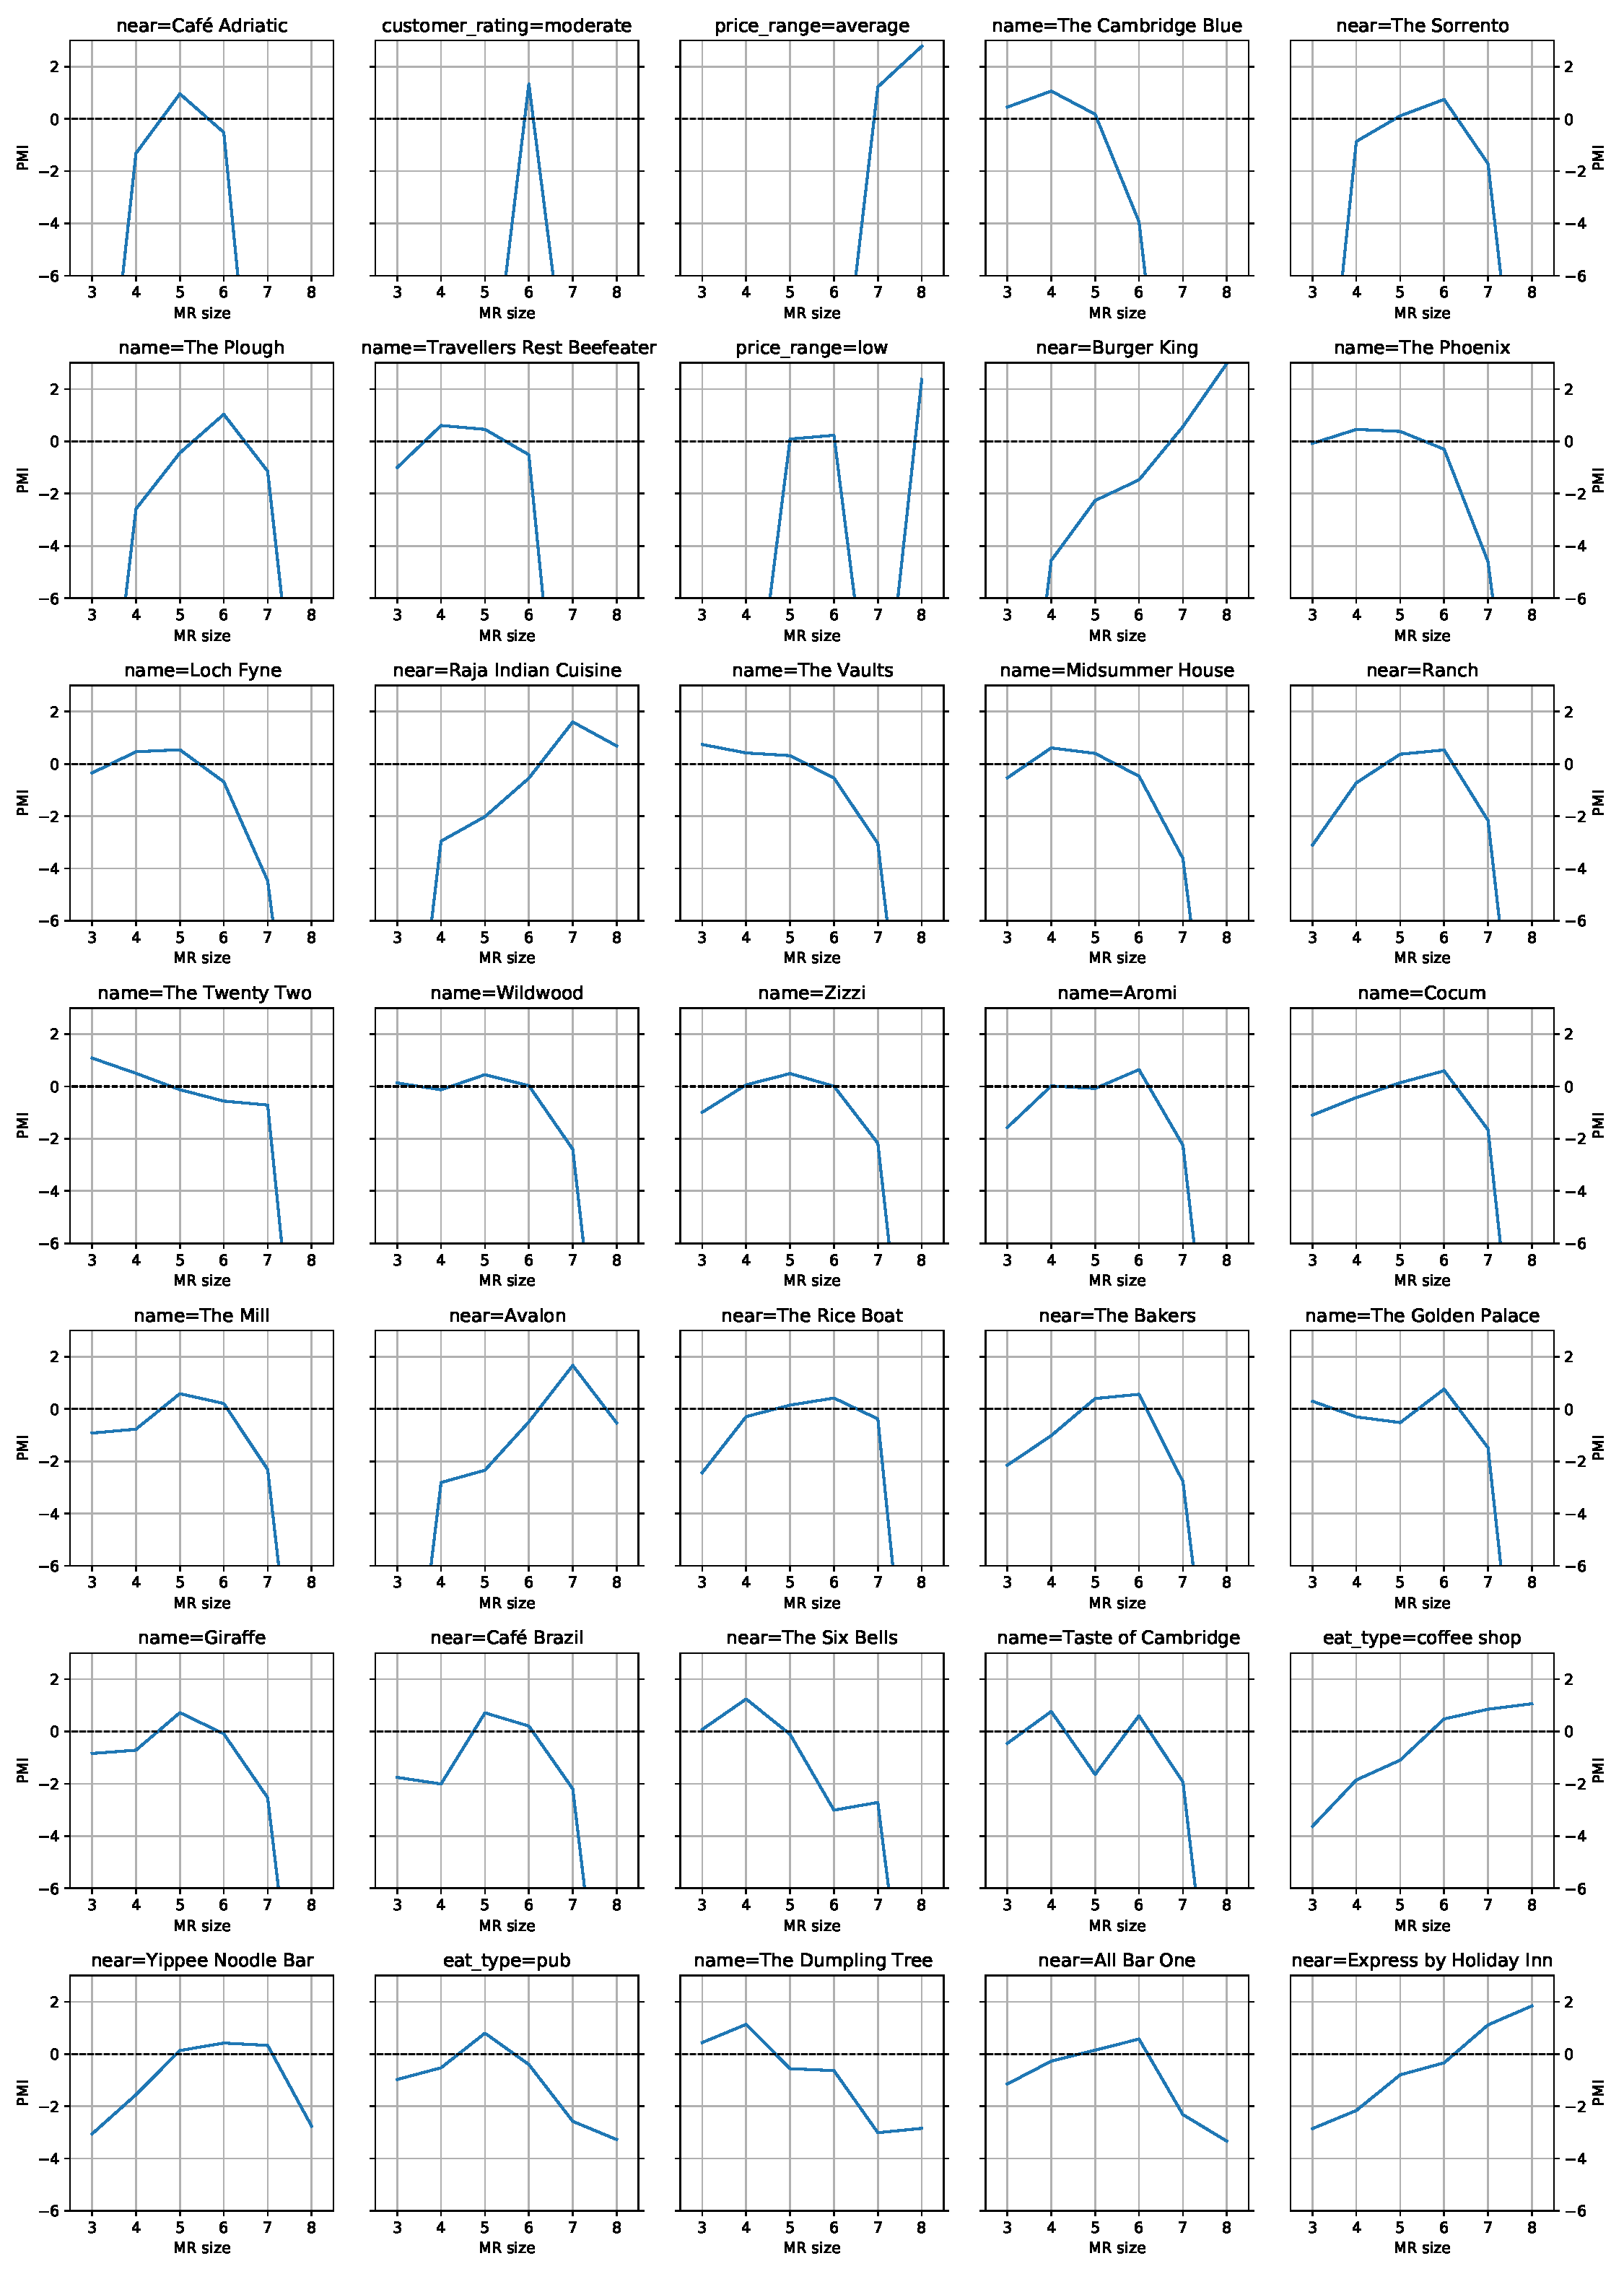
\includegraphics[width=\textwidth]{nlg/trainpmis.pdf}
\end{figure}


\clearpage
\subsection{Data-Augmentation: a Chicken and Egg Problem}

Ideally, we could follow the algorithm  sketched in \autoref{alg:idealda} 
and create synthetic
\meaningrepresentation/utterance pairs to add to our training data.

\begin{algorithm}[t]
$\augdata \gets \{\}$\\
\While{$\setsize{\augdata} < \numSamples$}{
$\tilde{\mr} \sim \daMrDist$ \\
$\boldsymbol{\tilde{\utttoks}} \sim \daUttDist(\boldsymbol{\tilde{\mr}})$\\
%\If{ $\lnot \filter(\tilde{\mr}, \boldsymbol{\tilde{\utttoks}})$}{ $\augdata \gets \augdata \cup \{(\tilde{\mr}, \boldsymbol{\tilde{\utttoks}}) \}$ }
$\augdata \gets \augdata \cup \{(\tilde{\mr}, \boldsymbol{\tilde{\utttoks}}) \}$
}
%    \KwResult{Salience judgements $\bsals = \left[ \bsal_1, \ldots, \bsal_\docSize\right]$}
$\gen_* \gets \operatorname{Train}(\corpus \cup \augdata)$\\
\KwResult{$\gen_*$}
    \caption{Idealized Data Augmentation and Training}
\label{alg:idealda}
\end{algorithm}

If the novel \meaningrepresentations~are drawn from a distribution, 
$\daMrDist$, such that $\daMrDist \ne \corpus_\mr$, 
and the novel utterances are generated from $\daUttDist(\tilde{\mr})$
 such that $\denotes{\boldsymbol{\tilde{\utttoks}}} = \tilde{\mr}$
while maintaining their fluency/naturalness (i.e., $\daUttDist \approx \corpus_\utttoks$),
then 
it is possible that that when training a \sequencetosequence~on the union 
of original training data and synthetic data, the resulting model, $\gen_*$,
 will behave
more systematically, which means more faithfully in our context.

Coming up with a reasonable data-augmentation 
\meaningrepresentation~distribution, $\daMrDist$, is fairly straightforward.
For example we could just sample the size of the \meaningrepresentation, $k$,
uniformly at random, then sample the $k$ \attributes~uniformly at random 
without replacement. Then for each of the attributes, values could be
sampled inversely proportional to their occurrence in the training data, i.e.
\begin{singlespace}
\begin{align*}
\operatorname{count}(a, v) & = \sum_{(\mr, \utttoks) \in \corpus} \mathds{1}\{\AV{$a$}{$v$} \in \mr  \}\\
k & \sim \operatorname{Uniform}(\{3, \ldots, 8\}) \\
p(v|a) & = \frac{\operatorname{count}(a,v)^{-1}}{\sum_{v^\prime \in {\mrvocab}_a}  \operatorname{count}(a,v^\prime)^{-1}} \\
a_i & \sim \operatorname{Uniform}(\{name, \ldots, near, eat\_type\}\setminus\{a_1,\ldots,a_{i-1}\}) & \forall i: i \in  \{1,\ldots, k\}\\
v_i & \sim p(\cdot|a) & \forall i: i \in \{1,\ldots,k\} \\
\tilde{\mr} & = \left[\!\!\left[ 
\begin{array}{c} 
\textsc{Inform} \\
\AV{$a_1$}{$v_1$} \\ \vdots \\ \AV{$a_k$}{$v_k$}  
\end{array}  
\right]\!\!\right]
\end{align*}\end{singlespace}
This procedure should produce valid \meaningrepresentations, and by 
definition $\daMrDist \ne \corpus_\mr$. Additionally, the co-occurance
of an \attribute~and a particular \meaningrepresentation~size will now be 
independent, and the co-occurrance of pairs of attributes will also be independent. 


Unfortunately, it is not clear how we implement utterance distribution
$\daUttDist(\mr)$ since if we had an utterance generation method that could
respond systematically to non-training data distributed \meaningrepresentations, we wouldn't need to perform data augmentation. As a starting point, 
we consider ways of generating samples from a base model $\gen_0$ which 
trained on the available training data, i.e. $\gen_0 = \operatorname{Train}(\corpus)$.

We cannot use $\gen_0$ with beam search as we saw previously,
there are some \meaningrepresentations~that $\gen_0$ won't be able to create utterances for (as we saw with \AV{near}{Burger King}). We could try a variant
of ancestral sampling, however 
it is difficult for ancestral sampling schemes to produce 
extremely different outputs without hurting fluency. 


\subsubsection{Noise Injection Sampling}

The fundamental issue with ancestral sampling is that the randomness of the
model at the word selection stage. This means that in the middle of generating
a phrase it is possible for a disfluent word to be selected, which can
disrupt the current phrase but also destabilize subsequent generation steps
as the model tries to recover from the unsual selection.
Ideally, randomness in a model would occur earlier in determining the 
``topicality'' or ``aboutness'' (you might even say content selection) 
of the generated utterance. Beyond the conditioning input $\ls(\mr)$,
the content that is to be generated is implicitly represented by
inner hidden states of the model. 

In \citet{cho}, they argue that the hidden states, $\decHidState_i$, 
of the \sequencetosequence~decoder lie on a manifold, as a requirement of
the linear separability of the next word prdecition, i.e.
$\gen(\utttok|\utttoks_{1:i},\ls(\mr)) \propto \exp \mathbf{w}_\utttok \cdot \decHidState_i$. The implication is that moving about the manifold will change 
the ``topicality'' of the distribution $\gen(\utttok|\utttoks_{1:i},\ls(\mr))$.
They further suggest adding Gaussian noise to $\decHidState_i$ as a way to
obtain stochastic samples from $\gen$. 

\newtcbox{\stochbox}[1][]{colframe=blue, colback=blue!15, boxrule=0.1mm,
                       nobeforeafter, tcbox raise base, shrink tight, extrude
                       by=0.32mm, #1}
\newtcbox{\detbox}[1][]{colframe=red, colback=red!15, boxrule=0.1mm,
                       nobeforeafter, tcbox raise base, shrink tight, extrude
                       by=0.32mm, #1}


\renewcommand{\algorithmcfname}{Alg.}

\begin{figure}[t]
\begin{center}\small \detbox{Deterministic operation}~~~~\stochbox{Stochastic operation}\end{center}
\resizebox{\textwidth}{!}{%
\begin{minipage}{0.33\textwidth}
\small
\begin{singlespace}
\begin{algorithm}[H]
$\encHidState_{1:\mrSize} \gets \operatorname{enc}(\ls(\mr))$\\
$\predutttok_1 \gets \starttok$\\
$\predutttoks \gets \left[ \predutttok_1\right]$\\
$i \gets 1$\\
\While{$\predutttok_i \ne \stoptok$}{
$\decHidState_i \gets \operatorname{dec}(\predutttoks, \encHidState_{1:\mrSize})$\\
$\vphantom{\boldsymbol{\epsilon_i} \sim \operatorname{Normal}(\zeroEmb, \frac{\sigma}{i})}$\\
\detbox{$\predutttok_{i+1} \gets \argmax_\utttok \gen(\utttok|\decHidState_i)$}\\
$\predutttoks \gets \predutttoks \oplus \left[ \predutttok_{i+1}\right]$\\
$i \gets i + 1$\\
}
%$\gen_* \gets \operatorname{Train}(\corpus \cup \augdata)$\\
\KwResult{$\predutttoks$}
    \caption{\small Greedy Decoding}
%\label{alg:idealda}
\end{algorithm}
\end{singlespace}
\end{minipage}\begin{minipage}{0.33\textwidth}
\small
\begin{singlespace}
\begin{algorithm}[H]
$\encHidState_{1:\mrSize} \gets \operatorname{enc}(\ls(\mr))$\\
$\predutttok_1 \gets \starttok$\\
$\predutttoks \gets \left[ \predutttok_1\right]$\\
$i \gets 1$\\
\While{$\predutttok_i \ne \stoptok$}{
$\decHidState_i \gets \operatorname{dec}(\predutttoks, \encHidState_{1:\mrSize})$\\
$\vphantom{\boldsymbol{\epsilon_i} \sim \operatorname{Normal}(\zeroEmb, \frac{\sigma}{i})}$\\
\stochbox{$\predutttok_{i+1} \sim \vphantom{\argmax_\utttok}\gen(\cdot|\decHidState_i)$}\\
$\predutttoks \gets \predutttoks \oplus \left[ \predutttok_{i+1}\right]$\\
$i \gets i + 1$\\
}
%$\gen_* \gets \operatorname{Train}(\corpus \cup \augdata)$\\
\KwResult{$\predutttoks$}
\caption{\small Ancestral Sampling}
%\label{alg:idealda}
\end{algorithm}
\end{singlespace}
\end{minipage}\begin{minipage}{0.38\textwidth}
\small
\begin{singlespace}
\begin{algorithm}[H]
$\encHidState_{1:\mrSize} \gets \operatorname{enc}(\ls(\mr))$\\
$\predutttok_1 \gets \starttok$\\
$\predutttoks \gets \left[ \predutttok_1\right]$\\
$i \gets 1$\\
\While{$\predutttok_i \ne \stoptok$}{
$\decHidState_i \gets \operatorname{dec}(\predutttoks, \encHidState_{1:\mrSize})$\\
\stochbox{$\boldsymbol{\epsilon_i} \sim \operatorname{Normal}(\zeroEmb, \frac{\sigma}{i})$}\\
\detbox{$\predutttok_{i+1} \gets \argmax_\utttok \gen(\utttok|\decHidState_i + \boldsymbol{\epsilon_i})$}\\
$\predutttoks \gets \predutttoks \oplus \left[ \predutttok_{i+1}\right]$\\
$i \gets i + 1$\\
}
%$\gen_* \gets \operatorname{Train}(\corpus \cup \augdata)$\\
\KwResult{$\predutttoks$}
\caption{\small Noise Injection Sampling}
%\label{alg:idealda}
\end{algorithm}
\end{singlespace}
\end{minipage}
}
\caption{A comparison of greedy decoding, ancestral sampling, and noise injection sampling.}
\label{fig:noiseinj}

%?\begin{minipage}{0.3\textwidth}
%?\begin{singlespace}
%?\begin{algorithm}[H]
%?$\predutttok_1 \gets \starttok$\\
%?$i \gets 1$\\
%?\While{$\predutttok_i \ne \stoptok$}{
%?$\tilde{\mr} \sim \daMrDist$ \\
%?%\If{ $\lnot \filter(\tilde{\mr}, \boldsymbol{\tilde{\utttoks}})$}{ $\augdata \gets \augdata \cup \{(\tilde{\mr}, \boldsymbol{\tilde{\utttoks}}) \}$ }
%?$\augdata \gets \augdata \cup \{(\tilde{\mr}, \boldsymbol{\tilde{\utttoks}}) \}$
%?}
%?%    \KwResult{Salience judgements $\bsals = \left[ \bsal_1, \ldots, \bsal_\docSize\right]$}
%?$\gen_* \gets \operatorname{Train}(\corpus \cup \augdata)$\\
%?\KwResult{$\gen_*$}
%?    \caption{Noise-Injection Sampling}
%?\label{alg:idealda}
%?\end{algorithm}
%?\end{singlespace}
%?\end{minipage}
\end{figure}





We show the noise injection sampling algorithm in \autoref{fig:noiseinj}
along with greedy decoding and ancestral sampling to emphasize the 
how the location of the stochasticity moves from the next word selection (line 8) to a peturbation of the hidden state (line 7). 
Note that in line 7 of the noise injection sampling algorithm, the standard
deviation of the normal distribution, $\frac{\sigma}{i}$, is scaled by the 
decoder step $i$ and in the limit turns to zero, i.e. $\lim_{i \rightarrow +\infty} \decHidState + \boldsymbol{\epsilon}_i = \decHidState$. The inuition 
behind this scaling is that we add the most noise at the first steps 
of decoding, which encourages the decoder to start from a topically novel
region of the hidden state manifold. As the decoding proceeds, the noise
reduces along with the chances of sending the decoder off the manifold
and destabilizing the decoding, and gradually we converge on the behavior of
greedy decoding. 

\begin{table}
    \centering
    \begin{tabular}{c ccc ccc ccc ccc ccc}
        \toprule
        $i$ & 1 & 2 & 3 & 4 &5 & 6 \\
        $\utttok_{i+1}$ &  the  & waterman &is &not& family & friendly \\
        \midrule
        $\gen(\utttok_{i+1}|\decHidState_i; \topkVocab{5}{i})$ & 0.874 & 0.004 & 0.380 & 0.397 & 0.915 & 0.147 \\
    $\gen(\utttok_{i+1}|\decHidState_i; \topkVocab{25}{i})$ &
0.792 & 0.004 & 0.344 & 0.371 & 0.877 & 0.147 \\
     $\gen(\utttok_{i+1}|\decHidState_i; \topkVocab{50}{i})$ &
0.778 & 0.004 & 0.339 & 0.366 & 0.872 & 0.147 \\
       $\gen(\utttok_{i+1}|\decHidState_i; \topkVocab{75}{i})$ &
0.772 & 0.004 & 0.338 & 0.364 & 0.870 & 0.147 \\
        $\gen(\utttok_{i+1}|\decHidState_i; \topkVocab{100}{i})$ & 
0.768 & 0.004 & 0.337 & 0.363 & 0.869 & 0.147 \\
        \midrule
     $\gen(\utttok_{i+1}|\decHidState_i; \nucleusVocab{.95}{i})$     & 
0.796 & 0.000 & 0.352 & 0.377 & 0.909 & 0.148 \\
     $\gen(\utttok_{i+1}|\decHidState_i; \nucleusVocab{.96}{i})$ &
0.789 & 0.000 & 0.349 & 0.374 & 0.898 & 0.148 \\
      $\gen(\utttok_{i+1}|\decHidState_i; \nucleusVocab{.97}{i})$ &
0.781 & 0.000 & 0.345 & 0.370 & 0.892 & 0.148 \\
     $\gen(\utttok_{i+1}|\decHidState_i; \nucleusVocab{.98}{i})$ &
0.773 & 0.000 & 0.342 & 0.367 & 0.882 & 0.148 \\ 
     $\gen(\utttok_{i+1}|\decHidState_i; \nucleusVocab{.99}{i})$ &
0.765 & 0.004 & 0.338 & 0.363 & 0.874 & 0.148 \\
        \midrule
        $\gen(\utttok_{i+1}|\decHidState_i)$ &0.758 & 0.004 & 0.335 & 0.359 & 0.865 & 0.147 \\
        $\gen(\utttok_{i+1}|\decHidState_i + \boldsymbol{\epsilon}_i)$ & 0.321 & 0.170 & 0.408 & 0.489 & 0.785 & 0.514 \\
        \bottomrule
    \end{tabular}

~\\~\\~\\~\\


    \begin{tabular}{c ccc ccc ccc ccc ccc}
        \toprule
        $i$             & 7  & 8 & 9 & 10 & 11 & 12 & 13 & 14 \\
        $\utttok_{i+1}$ &  and &is& located &near& burger & king & . & \stoptok \\
        \midrule
 $\gen(\utttok_{i+1}|\decHidState_i; \topkVocab{5}{i})$ &  0.338 & 0.111 & 0.147 & 0.168 & 0.000 & 0.954 & 0.931 & 0.810 \\
 $\gen(\utttok_{i+1}|\decHidState_i; \topkVocab{25}{i})$ & 0.327 & 0.101 & 0.111 & 0.148 & 0.001 & 0.935 & 0.911 & 0.810 \\
 $\gen(\utttok_{i+1}|\decHidState_i; \topkVocab{50}{i})$ & 0.326 & 0.100 & 0.105 & 0.146 & 0.001 & 0.930 & 0.910 & 0.810 \\
 $\gen(\utttok_{i+1}|\decHidState_i; \topkVocab{75}{i})$    & 0.326 & 0.100 & 0.103 & 0.145 & 0.001 & 0.928 & 0.909 & 0.810 \\
 $\gen(\utttok_{i+1}|\decHidState_i; \topkVocab{100}{i})$ & 0.326 & 0.100 & 0.102 & 0.144 & 0.001 & 0.926 & 0.909 & 0.810 \\
        \midrule
   $\gen(\utttok_{i+1}|\decHidState_i; \nucleusVocab{.95}{i})$      & 0.342 & 0.104 & 0.103 & 0.150 & 0.000 & 0.964 & 0.950 & 0.810 \\
   $\gen(\utttok_{i+1}|\decHidState_i; \nucleusVocab{.96}{i})$ & 0.338 & 0.103 & 0.102 & 0.149 & 0.000 & 0.954 & 0.939 & 0.810 \\
$\gen(\utttok_{i+1}|\decHidState_i; \nucleusVocab{.97}{i})$
     & 0.333 & 0.102 & 0.101 & 0.148 & 0.000 & 0.947 & 0.931 & 0.810 \\
 $\gen(\utttok_{i+1}|\decHidState_i; \nucleusVocab{.98}{i})$   
     & 0.332 & 0.101 & 0.100 & 0.146 & 0.000 & 0.937 & 0.924 & 0.810 \\
 $\gen(\utttok_{i+1}|\decHidState_i; \nucleusVocab{.99}{i})$
     & 0.329 & 0.100 & 0.099 & 0.145 & 0.001 & 0.928 & 0.917 & 0.810 \\
 \midrule
        $\gen(\utttok_{i+1}|\decHidState_i)$ & 0.326 & 0.099 & 0.098 & 0.143 &0.001 & 0.919 & 0.908 & 0.810\\
        $\gen(\utttok_{i+1}|\decHidState_i + \boldsymbol{\epsilon}_i)$ & 0.459 & 0.562 & 0.440 & 0.731 &0.599 & 0.972 & 0.903 & 0.984 \\
 \bottomrule
    \end{tabular}

    \caption{Word selection probabilities when using ancestral sampling,
        top-$k$ sampling (for $k \in \{5,25,50,75,100\}$), 
    nucleus samplling (for $\nucleusthr \in \{0.95, 0.96, 0.97, 0.98, 0.99\}$), and noise-injection sampling ($\sigma = 2.0$).}
    \label{tab:sampprobs}
\end{table}




We can understand noise injection sampling as a compromise between
greedy decoding and ancestral sampling; rather than draw a sequence of utterance
tokens stochasticity, we instead draw a sequence of hidden state spaces.
Given the sequence of hidden state spaces, the corresponding sequence of
utterance tokens is deterministically decided by the most likely next token
given the last hidden state. This next word selection strategy helps to
avoid disfluent continuations.


In \autoref{sample examples}, we show examples of samples obtained with
noise injection sampling as well as some ancestral sampling schemes.
We can see that the ancestral sampling examples are not very diverse,
and occassionally contain disfluencies. The noise injection sampling
example, however, semantically diverges from the input while maintaining
fluency. It was even able to generate an utterance containing the phrase
``near Burger King'' which is was practically impossible to generate with
beam search.


In \autoref{tab:sampprobs}, we show the probability of generating this example
under the various sampling schemes. In our present case, top-$k$ and nucleus
sampling have very similar distributions to the ancestral sampling
distribution ($\gen(\utttok_{i+1}|\decHidState_i)$). All three of these 
techniques assign a very low probability to generating the example utterance,
and in the case of nucleus sampling, it only gives non-zero probability when
using a nucleus of 0.99 cumulative probability (i.e. $\nucleusVocab{.99}{i}$)!
In particular, noise injection sampling puts much more probability 
mass on generating relatively rare \attributevalue~realizations ($i=2$, ``waterman'' and $i=11$, ``burger'').








\subsubsection{Practical Data-Augmentation Scheme}



\newtcbox{\truttbox}[1][]{colframe=green, colback=green!15, boxrule=0.1mm,
                       nobeforeafter, tcbox raise base, shrink tight, extrude
                       by=0.32mm, #1}
\newtcbox{\mrdistbox}[1][]{colframe=orange, colback=orange!15, boxrule=0.1mm,
                       nobeforeafter, tcbox raise base, shrink tight, extrude
                       by=0.32mm, #1}

\newtcbox{\ninjbox}[1][]{colframe=purple, colback=purple!15, boxrule=0.1mm,
                       nobeforeafter, tcbox raise base, shrink tight, extrude
                       by=0.32mm, #1}
\newtcbox{\correctbox}[1][]{colframe=blue, colback=blue!15, boxrule=0.1mm,
                       nobeforeafter, tcbox raise base, shrink tight, extrude
                       by=0.32mm, #1}
\newtcbox{\filterbox}[1][]{colframe=cyan, colback=cyan!15, boxrule=0.1mm,
                       nobeforeafter, tcbox raise base, shrink tight, extrude
                       by=0.32mm, #1}

\newtcbox{\returnbox}[1][]{colframe=violet, colback=violet!15, boxrule=0.1mm,
                       nobeforeafter, tcbox raise base, shrink tight, extrude
                       by=0.32mm, #1}

\begin{figure}[t]
\begin{singlespace}
\begin{algorithm}[H]
\truttbox{$\gen_0 \gets \operatorname{Train}_\utttoks\left(\corpus\right)$} \\
\truttbox{$\dmodel \gets \operatorname{Train}_\mr\left(\corpus\right)$} \\
$\augdata \gets \left\{ \right\}$\\
\While{$\setsize{\augdata} < \numSamples$}{
\mrdistbox{$\samplmr \sim \pdaMrDist$}\\
\ninjbox{$\pdaCandUtts\gets \left\{ \pdaCandUtt \sim 
            \gen_0\left(\cdot|\ls(\samplmr), \pdaCandEps\right) 
            \quad \forall i : i \in \{1,\ldots, k\} \right\} $}\label{lst:pdacand}\\
\ninjbox{$\predutttoks \gets
    \argmax_{\pdaCandUtt \in \pdaCandUtts} 
    \frac{\log \gen_0\left(\pdaCandUtt|\ls(\samplmr),\pdaCandEps \right)}{\setsize{\pdaCandUtt}}$}\label{lst:pdacandselect}\\
\correctbox{$\pdaPredMr \gets \dmodel\left(\predutttoks\right)$}\\
\If{\filterbox{$\lnot \operatorname{Filter}\left(\pdaPredMr, \predutttoks\right)$}}{
    $\augdata \gets \augdata \cup \left\{ \left(\pdaPredMr, \predutttoks\right) \right\}$
}
~\\
}
\returnbox{$\gen_1 \gets \operatorname{Train}_\utttoks(\corpus \cup \augdata)$}\\
\KwResult{$\gen_1$}
    \caption{Data Augmentation with Noise-Injection Sampling and Self-Training }
%\label{alg:idealda}
\end{algorithm}
\end{singlespace}
\caption{A comparison of greedy decoding, ancestral sampling, and noise injection sampling.}
\label{fig:practda}
\end{figure}


Because of its ability to generate semantically divergent and novel
outputs while maintaining fluency, we adopt this noise injection
sampling as our method of sampling utterances, $\daUttDist$, for 
data-augmentation. We show our actual data-augmentation scheme in
\autoref{fig:practda} and now walk through some of the implementation details.

\paragraph{\truttbox{Train base generator $\gen_0$ and \meaningrepresentation~parser $\dmodel$.}}
The algorithm begins by training the base generator, i.e. na{\"i}ve 
\sequencetosequence~model, and \meaningrepresentation~parser $\dmodel$. 
Both models are trained on the same data, with the only real change to the 
$\operatorname{Train}$ sub-routine being which part of a training example
is the ouput and which is the input. Alternatively, $\dmodel$ can 
also be implemented using regular-expression-based rules. We defer detailed 
explanation of $\dmodel$ until the experiments; it suffices to understand
$\dmodel$ as a mapping from utterances to \meaningrepresentations.




\paragraph{\mrdistbox{Sampling a \meaningrepresentation, $\samplmr$}}
Move sampling stuff from above to here.

\paragraph{\ninjbox{Generating a novel utterance with noise-injection 
    sampling.}}
    In \autoref{lst:pdacand} we take $k$ noise-injection samples to construct
    a candidate set of utterances, $\pdaCandUtts$. From $\pdaCandUtts$ we
    select as our noise-injection sample, the utterance $\predutttoks$
    which has the highest average token log-likelihood (\autoref{lst:pdacandselect}). We do this selection step so as to be extra cautious and avoid adding
    any potentially disfluent utterance. 
    
    \paragraph{\correctbox{Predict \meaningrepresentation~$\pdaPredMr$ from
    $\predutttoks$.}} Because the noise-injection sampling produces highly
semanticly deivergent utterances, it is unlikely that $\denotes{\predutttoks } = \samplmr$. Instead we use the \meaningrepresentation~parser, $\dmodel$, to
recover the most likely \meaningrepresentation, $\pdaPredMr = \dmodel\left(\predutttoks\right)$.

\paragraph{\filterbox{Check synthetic datapoint $(\pdaPredMr,\predutttoks)$.}}
We do one last quality check on the synthetic example $(\pdaPredMr,\predutttoks)$ before adding it to the augmented dataset, $\augdata$. We make sure that
the probability of $\pdaPredMr$ under $\dmodel$ is above a threshold when using
a model-based \meaningrepresentation~parser. When using a rule-based
\meaningrepresentation~parser, we check to make sure that there are no
repeated \attributevalue-pairs in $\predutttoks$, e.g., ``Aromi is a 
coffee shop and it is a coffee shop.'' If the \meaningrepresentation/utterance
pair passes these final quality checks, we add it to $\augdata$.

\paragraph{\returnbox{Train an augmented generator $\gen_1$ on $\corpus \cup \augdata$.}} After generating a dataset of synthetic data, we train a new 
generation model, $\gen_1$, on the union of the original training data
and the newly generated synthetic data. We refer to this model as 
the augmented generator and as we will show empirically, the augmented
model is more faithful than the base generator, $\gen_0$.
We call this process self-training because the $\gen_1$ and $\gen_0$ share 
the same architecture, and $\gen_1$ is trained on data produced by $\gen_0$.

\section{Experiments}

We experimentally validate the noise-injection sampling and self-training
data-augmentation scheme on the E2E Challenge dataset~\citep{something} 
and the Laptops and TVs datasets \citep{wen}, three collections of 
\meaningrepresentation/utterance pairs for training response generation models

\naturallanguagegeneration~models for t

\subsection{Datasets}

We use three recent dialogue generation datasets in our experiments,
the E2E Challenge Dataset \cite{duvsek2019evaluating}, and the Laptops and 
TVs datasets \cite{wen2016multi}.
We only briefly review them here.
Each dataset consists of \meaningrepresentations~paired with one or more 
reference utterances.
%(see \autoref{figure:introexample} for an example from the E2E dataset).
%The structure of each \meaningrepresentation~is relatively simple, 
%consisting of the 
%dialog act itself, (e.g. \textit{inform}, \textit{recommend}, 
%\textit{compare}, etc.) and a variable number of attribute slots
%which need to be realised in the utterance. 
All attribute values 
come from a closed vocabulary.
%If an attribute is not present in the MR it should not be realized in the 
%corresponding utterance. 

The three datasets also represent different training size conditions; 
with the E2E Challenge dataset representing the ``large data'' training
condition and the Laptops and TVs dataset representing ``small data'' conditinos. See \autoref{datasizes} for dataset size statistics.
The E2E Challenge dataset has only one dialogue act, \textsc{Inform}, 
and its training \meaningrepresentations~contain three to eight
\attributes~unique attributes. 
The Laptops and TVs datasets contain a more diverse set of \meaningrepresentation/utterance pairs. There are {\color{red}???} unique dialogue acts. 
The number of minimum and maximum \attributes~varies according to the dialogue
act. See \autoref{avdeets} for detailed statistics of the dialogue acts
and \attributevalue~pairs for the three training sets. 


\paragraph{Delexicalization}
Prior work using neural \naturallanguagegeneration~models often relies on 
delexicalization, that is, replacing realizations of named-entity or 
numeric values in an utterance with a placeholder token, in order to alleviate
data sparsity issues and yield better generalization when a generating utterances about named-entities not seen in the trianinig dataset. For example
on the E2E Challenge dataset, the \Atr{name}~and \Atr{near}~attributes
are often delexicalized because they are proper names of estabilishments
that are simple to find and replace in the utterance.

For example, the fully lexicalized utterance 

\begin{center}\noindent~~~~\textit{Near The Six Bells is a venue that is children
friendly named The Golden Curry.}\end{center}

\noindent can be delexicalized as

\begin{center}\noindent ~~~~\textit{Near <<near>> is a venue that is children
friendly named <<name>>.}\end{center}

Delexicalized utterances can be re-lexicalized as a post-processing
step, where the placeholder token is replaced with the correct value text.

On the E2E Challenge dataset, we experiment with delexicalization of the 
\textit{Name} and \textit{Near} attributes since thah have a relatively large vocabulary of valid slot fillers, some of which are only seen  infrequently in the training data;
it can be difficult for fully lexicalized models to produce some of the 
rarer location names for these attributes. 

However, since delexicalization might be difficult or 
impossible in other domains, we implement both delexicalized and lexicalized
versions of the generation models on the E2E dataset to 
more fully evaluate the
self-training method.
   

The evaluation script for the Laptops and TVs datasets uses delexicalization
to evaluate attribute realization error, and so we use it here to be 
consistent with prior work, 
delexicalizing all possible attributes.
%



\subsection{Generation Models}

We use a two-layer, unidirectional GRU architecture with Bahdanau style
attention for our 
\sequencetosequence~model. We set $\embDim = \hidDim = \encDim = \decDim = 512$, that is, we use 512-dimensional embedding and hidden states.

We fit model parameters, $\params$, by minimizing the negative log-likelihood
of the training set, $\corpus$, i.e. $\mathcal{L}(\params) = - \sum_{(\mr, \utttoks) \in \corpus  }  \log \gen\left(\utttoks|\ls(\mr);\params\right).$
When generating utterances for evaluation (i.e. not for use in noise-injection sampling) we use either greedy decoder or beam decoding with a 
beam size of eight.
The beam search terminates after eight candidates have been generated;
the candidates are reranked by average token log-likelihood, $\frac{\log \gen\left(\utttoks|\ls(\mr)\right)}{\setsize{\utttoks}}$. In these experiments, we \textbf{do not} use a discriminative reranker to ensure the faithfulness of the 
selected beam candidate. 

\subsection{\MeaningRepresentation~Parsing Models}

Given a novel utterance $\predutttoks$~sampled from $\gen$, we need to 
reliably parse the implied \meaningrepresentation, i.e. 
$\pdaPredMr = \dmodel(\predutttoks)$, 
where \dmodel~is our parsing model. We have two things going for us in 
our experimental setting. First, even with noise injection sampling,
model outputs are fairly patterned, reducing the variability of the utterances
we need to parse in practice. 

Second, the \meaningrepresentation~in this study are
flat lists of attributes that are somewhat independent of each other.
We only need to detect the presence of each attribute and its value.
For the Laptops and TVs datasets we also need to recover the dialog
act but these also are signaled by a fairly limited repertoire 
of cues, e.g. ``we recommend.'' % or ``compared to'' for the 
%\textit{Recommend} and \textit{Compare} DAs respectively. 
Given this, we experiment with both hand crafted regular expression 
rules and learned classifiers to predict the value of
an attribute if present or that it is missing. 


\paragraph{Rule-based parser (\ruledmodel)} We design hand-crafted 
regular expression based rules to match for the presence of key phrases 
for each of the attributes and DAs in the datasets while also checking to
make sure that there is only one match per attribute.

To construct the rules, we look through both the training data references as 
well as the generation model outputs as this is what the rules will
be operating on in practice. For each lexicalized attribute (and DA) we 
develop a list of regular expressions % or conjunctions of regular expressions
such as,
\texttt{/is (family|kid|child) friendly/} $\Rightarrow$ \textit{familyFriendly[yes]}.
For the delexicalized attributes, we simply check for the presence 
of the placeholder token. 

%One failure mode of the generation models on
%Laptops and TVs is to use the wrong attribute value token in an expression,
%e.g. ``...has a DRIVESIZERANGE price range,'' so we add additional rules
%to mark an utterance/MR pair as invalid in these cases.
%e.g.
%\begin{align*}
%\texttt{/price/}~\land~\lnot\texttt{/PRICERANGE/} 
%    \Rightarrow \emptyset.
%\end{align*}

We design these rules to be high precision, as it is safer to miss out on 
more obscure varieties of utterance to avoid adding incorrectly parsed data 
points.
However,  in many cases the rules are also high recall as well. 
The average F-score on the E2E validation set is 0.93.
%In some cases, this is probably
%close to the performance ceiling; the human authored references in the validation
%set are noisy and are often incorrectly labeled or omit realizing attributes.


%This is a relativity conservative approach as it is possible we will
%miss good phrases, however, it is more important that we add as little
%noise to augmented dataset as possible.
%rules to detect the presence of 
%key phrases related to each attribute's realization. We design these rules
%to be high-precision, so even while we may not cover all possible 
%only need to augment our training data with pairs $(\samplex, \sampley)$ 
%If the rules indicate that the MR is valid (e.g. only mentions an attribute
%once). While we may miss out on more diverse constructions, we more reliably
%ensure the augmented data is correct, i.e. \sampley~correct conveys the
%discourse act and attibute values specified in \samplex. Adding too many
%incorrect pairs will degrade the reliability of our final generation model.



\paragraph{Classifier-based parser (\learndmodel)} 
It is perhaps too optimistic to believe we can construct reasonable rules
in all cases. Rule creation quickly becomes tedious and for more complex
MRs this would become a bottleneck. To address these concerns, we also 
study the feasibility of using learned classifiers to predict the presence
and value of the attributes. For each attribute in the E2E dataset,
we trained a separate convolutional neural network (CNN) classifier 
to predict the correct attribute value (or \textit{n/a} if the attribute is 
not present).
The CNN architecture follows that of \citet{kim2014convolutional} and is 
trained with 
gradient descent on the original training data. 



We use a separate CNN classifier for each attribute to predict
the corresponding value (or \textit{n/a}) from an utterance $\utttoks$.
We first look up the tokens in $\utttoks$ in an embedding matrix $E$
to obtain a matrix $W\in\mathbb{R}^{N \times D}$ where $D=50$ is
the embedding dimension.

We then apply a series of unigram, bigram, and trigram convolutional
filters each with $50$ output features.
After concatenating and max-pooling over the sequence dimension,
and applying a ReLU activation,
we obtain a hidden layer in $\mathbb{R}^{150}$.
We then apply another fully-connected layer with ReLU activation
which down projects the hidden layer to $\mathbf{R}^{50}$.
Finaly we apply the final softmax layer to predict the class label.

During training we apply dropout (with drop rate 0.25) to 
the embedding layer, convolutional filter outputs, and hidden
layers. We train for 30 epochs with gradient descent
using  a learning rate of 0.25 and 
weight decay penalty of 0.0001, using validation set F1
as our model selection criterion.
The average E2E validation F-score is 0.94.
%iThe classifiers
%required significantly less manual effort
%(and almost zero domain knowledge) to construct.

\subsection{E2E Challenge Self-Training Experiments}
 We train base generators $\basegen$~on the original training data $\corpus$, 
 with and without
delexicalizing the \textit{Name} and \textit{Near} attributes. 
We train for 500 epochs with gradient descent. We use a batch size of 128,
with a learning rate of 0.25, weight decay penalty of 0.0001, and a dropout 
probability of 0.25.
We select the best model iteration using validation
set BLEU score\footnote{We use the official shared task script to
compute automatic quality metrics on the E2E dataset.}.

Using the self-training method outlined in \autoref{section:selftrain},
we create augmented datasets using either $\learndmodel$~or
$\learndmodel$, which we refer to as 
$\augdata_{\ruledmodel}$ and $\augdata_{\learndmodel}$ respectively 
($\learndmodel$~is only in the delexicalized setting).

To sample a novel MR with  $S$ attributes, we sample a combination of $S-1$ attributes
uniformly at random %from the $\binom{7}{S-1}$ possible combinations
(always appending the \textit{name} attribute since every MR contains it).
 We 
then sample attribute values for each slot % independently
inversely proportional to their empirical frequency
in the training set so as to increase the likelihood of creating a novel
or under-represented MR.


After obtaining such a sample $\utttoks$~we then perform noise injection sampling,
generating 200 samples $\pdaCandUtt \sim 
\basegen(\cdot|\utttoks, \epsilon^{(i)})$ 
in parallel and discarding all but the top 20
samples by average log likelihood according to $\basegen$.
We also discard any utterances that have previously been generated.
%to avoid 
%adding repeat utterances to the augmented data.

We then apply the parser to the sampled utterances, to obtain its
predicted MR, $\pdaPredMr^{(i)} = \dmodel(\pdaCandUtt)$. If using 
the rule based parser $\ruledmodel$~and $\pdaPredMr^{(i)} 
= \emptyset$, i.e. the utterance
does not have a valid parse, we discard it.
Similarly, when using the classifier based parser, \learndmodel, if 
any attribute value is predicted with less than 50\% probability we discard 
it. All surviving $(\pdaPredMr^{(i)}, \predutttoks^{(i)})$ pairs are added to \augdata.
We repeat this process 25,000 times for each valid MR size $S$.
See \autoref{table:samplequal} for statistics on the total sample sizes 
after filtering.
%yielding 1,591,788 additional samples for the lexicalized \basegen/\ruleclf,
%501,909 for the delexicalized \basegen/\ruleclf, and 384,436 for the 
%delexicalized \basegen/\learnedclf~pairings.

\

For both $\corpus \cup \augdata_{\ruledmodel}$ and 
$\corpus \cup \augdata_{\learndmodel}$ we train new generators \auggen~using 
the same training setting as above (although we terminate training after 50 
epochs
because the models converge much faster with the additional data).

We report BLEU, ROUGE-L, and METEOR on the E2E test set.
We show results for both greedy and beam decoding with beam size 8
under $\basegen$~and
\auggen~models. We compare our models to the best sequence-to-sequence DNN
model, Slug \cite{juraskaslug2slug}, the best grammar rule based model, 
DANGNT \cite{nguyen2018structurebased},
and the best template based model, TUDA \cite{puzikov2018e2e}, as determined during 
the shared task evaluation \cite{duvsek2019evaluating}.


%We then create augmented datasets using the methods
%described in section~\ref{}, using either the rule-based classifier 
%\ruleclf~or learned classifier \learnedclf~to reconstruct the MRs.
%For each filtering method we train a new generator \auggen~on the union of 
%the original training data the augmented data collection, i.e. 
%$\trdata \cup \augdata^{\ruleclf}$ and $\trdata \cup \augdata^{\learnedclf}$.
%The architecture of \auggen ~ is identical to that of \basegen. We 
%train \auggen ~ for 50 epochs (with the added data, the \auggen ~ 
%models converge much faster), again selecting the best model via validation 
%set BLEU score.

\subsection{Laptops and TVs Self-Training}
We perform similar experiments on the Laptops and TVs datasets. 
We train a separate \basegen~model for each dataset 
for 300 epochs with a learning rate of 0.1
for Laptops and 0.25 for TVs. The weight decay penalty was 0.0001 
and dropout probability was 0.25. Best model iteration is determined
by validation set BLEU score. As in the E2E experiments, we create an augmented
dataset for both the Laptops and TVs dataset using the method
outlined in \autoref{section:selftrain}. We then train new generators 
\auggen~on the union of original training data and the augmented dataset.

On the Laptops and TVs dataset,
%each DA can have a different minimum and maximum number of attributes.
for each DA and legal number of attributes $S$ we draw $S$ random attributes
(modulo any required attributes like \textit{Name}; not all DAs require it).\footnote{A number of attributes $S$ is ``legal'' if we observe a DA instance with that 
many attributes in the original training data.}
%For binary attributes, or attributes that can have the \textit{don't care}
%value, we randomly sample these values, to obtain a MR \mrx.

We then perform noise injection sampling,
generating 200 samples $\pdaCandUtt \sim 
\basegen(\cdot|\mrtoks, \epsilon^{(i)})$ under the same settings as the E2E
dataset. We repeat this process 25,000 times for each DA and DA size.
We obtain 373,468 and 33,478 additional samples for the Laptops 
and TVs datasets respectively.


We automatically evaluate our models using the evaluation script of
\citet{wen2016multi}, which computes BLEU scores, as well as slot
alignment error rate (since this dataset is almost fully delexicalized,
it simply checks for the presence of the correct attribute placeholders
according to the MR). We compare again to the Slug model as well
as the Semantically Conditioned LSTM (SCLSTM) \cite{wen2015semantically}
which report state-of-the-art results on these datasets.


\begin{table}
\centering
\begin{tabular}{rcccc}
\toprule
Model  & BLEU & R.-L & MET. \\ \midrule
Slug   & 66.19 & 67.72 & 44.54  \\  
DANGNT & 59.90 & 66.34  & 43.46  \\
TUDA   & 56.57 & 66.14  & 45.29  \\
        \midrule
delex. \basegen~~~~~~greedy & 66.91 & 68.27 & 44.95 \\
                      beam & \textbf{67.13} &  \textbf{68.91} &  45.15  \\
        \auggen~\ruleclf~greedy   &  65.57 & 67.71 & 45.56  \\
                             beam & 66.28 &  68.08 &  \textbf{45.78}  \\
     \learnedclf~greedy & 63.76 &  67.31 &  44.94  \\
   beam   & 
 64.23 &  67.54 &  45.17  \\
\midrule
   lex. \basegen~~~~~~greedy & 60.35 &  64.51 & 41.82  \\
                      beam   & 61.81 &  65.83 & 42.69  \\
    \auggen~\ruleclf~greedy & 64.74 &  68.21 & 44.46  \\
       beam & 64.81 &  67.83 &    44.39  \\
\bottomrule
\end{tabular}
\caption{BLEU, ROUGE-L, and METEOR metrics on the E2E test set. Baseline methods all rely
on at least partial delexicalization, puting our lexicalized models at a relative disadvantage.}

\label{table:autoqual}
\end{table}





\begin{table*}
\setlength{\tabcolsep}{5pt}
\center
  \begin{tabular}{rrrr ccccc ccc ccc}
    \toprule
 \multicolumn{4}{c}{
\multirow{2}{*}{
Model} }
       & \multirow{2}{*}{Name} & \multirow{2}{*}{Near}    
            &  Family  & 
           \multirow{2}{*}{Area}    & Customer & \multirow{2}{*}{Food} 
      & Price & Eat & \multirow{2}{*}{All} \\
  & & & &  &  & Friendly & 
        & Rating &  & Range & Type &  \\
\midrule
\multicolumn{4}{r}{Slug}  
                    & 0 & 0 & 6  & 1  & 6  &  10  & 35  & 9  & 67 \\ 
\multicolumn{4}{r}{DANGNT}
                    & 0 & 0 & 18  & 0  & 0  & 0  & 0  & 58  & 76 \\ 
\multicolumn{4}{r}{TUDA}  
                    & 0 & 0 & 0  & 0  & 0  & 0  & 0  & 0    & \textbf{0} \\
\midrule
delex. & \basegen & & greedy 
                    & 0   & 0   & 23 & 23 & 16 & 26 & 27 & 0 & 115 \\ 
& & & beam          & 0   & 0   & 60 & 3  & 9  & 3  & 8  & 0 & 83  \\ 
& \auggen & \ruledmodel & greedy 
                    & 0   & 0   & 0  & 0  & 0  & 0  & 0  & 0 & \textbf{0} \\ 
 & & & beam         & 0   & 0   & 0  & 0  & 0  & 0  & 0  & 0 & \textbf{0} \\
 & & \learndmodel & greedy 
                    & 0   & 0   & 1  & 0  & 8  & 1  & 9  & 0 & 19 \\
 & &  & beam        & 0   & 0   & 0  & 0  & 3  & 0  & 0  & 0 & 3 \\
\midrule
lex. & \basegen & & greedy 
                    & 145 & 141 & 14 & 15 & 2   & 14 & 2  & 0 & 333 \\
 & & & beam         & 155 & 124 & 62 & 0  & 0   & 0  & 0  & 0 & 341 \\ 
 & \auggen & \ruledmodel  & greedy 
                    & 0   & 0   & 2  & 0  & 0  & 125 & 0  & 0 & 127 \\
&  &  & beam        & 0   & 2   & 0  & 0  & 0  & 119 & 0  & 0 & 121 \\
\bottomrule
    \end{tabular}
\caption{Attribute realization errors on the E2E test set. The Slug model and our delexicalized models delexicalize the NAME and NEAR slots, 
    thus making 0 errors on these attributes. DANGNT and TUDA models perform complete delexicalization. } 
\label{table:autosem}
\end{table*}






\subsection{E2E Challenge Results}

Surprisingly, \basegen~using greedy decoding surpases all of the 
baseline systems. This is quite shocking as the Slug model ensembles
three different sequence-to-sequence models producing 10 outputs each using beam search and reranking based on slot alignment to select the final generation
output. The $\auggen$/$\ruledmodel$~model remains competitive with Slug, 
again even using greedy decoding.
The $\auggen$/$\learndmodel$~starts underperforming Slug on BLEU score but
remains competitive on ROUGE-L and METEOR again when using greedy decoding.
Overall the augmented training data tends to hurt generation quality.
In this regard, the added noise of the trained classifier exacerbates things
as it reduces quality more than the rule-based filtering. 

In the lexicalized setting,
$\basegen$~produces lower quality output than the Slug system.
However, the augmented training procedure increases
the quality of the lexicalized $\auggen$~model which beats Slug on ROUGE-L.


The automatic quality evaluations are somewhat limited, however. To gain
more insight into model performance
we apply our rule based parser to estimate attribute realization error
for all system outputs on the test set,
similarly to \cite{duvsek2019evaluating}
(e.g., if the MR specifies \textit{food[French]},
we check to make sure the generated utterance says so). 
The results of this evaluation are shown in \autoref{table:autosem}.
Immediately, it is revealed that \basegen~is far worse than the baseline 
methods making 115 and 83 errors using greedy and beam decoding respectively.


The $\auggen$/$\ruledmodel$~model achieves zero test set
errors even when using the greedy 
decoding. The $\auggen$/$\learndmodel$~model is slightly worse (in agreement 
with the automatic quality measurements), but its greedy search is still
superior to the more sophisticated Slug decoder, achieving 19 total
test set errors compared to Slug's 67 errors.



The lexicalized $\basegen$~model has especially high error rates, 
particularly on the \textit{Name} and \textit{Near} attributes.
With augmented data training, the $\auggen$~model reduces these errors
 to zero when using greedy search and 2 with beam search. Unfortunately,
the augmented training is more unstable in the lexicalized setting, 
as it produces a large spike in \textit{food} attribute errors, although
the $\auggen$~models still have lower overall error than  $\basegen$.


\subsection{Laptops and TVs Results}
The results are more mixed here. Our BLEU scores are about 15 points 
below the baselines on the Laptops dataset and 20 points below the 
baselines on the TVs dataset. 
Upon examing  the evaluation script in detail we see that 
BLEU score is calculated using 5 model outputs which \citet{juraskaslug2slug}
and \citet{wen2016multi} do. We only produce the 1-best output
at test time,
perhaps explaining the difference.

Looking through our model
outputs we see mostly good utterances, often nearly exactly matching the 
references.
Our models outperform the state of the art models on errors. The best state of the art models  make errors by generating sentences that do not match the input representation 0.79\%  and 1.67\% of the time on the Laptops and TVs datasets
respectively. Our \auggen~model reduces that error to only 0.13\% and 
0.20\%.

%We do achieve the lowest error rates, with \auggen~beam
%decoding achieving a 0.2\% error rate versus the previous best of 1.67\%
%on the TVs dataset, and \auggen~greedy decoding achieving a 0.13\% error
%rate compared the 0.79\% baseline rate.



\begin{table}
    \begin{tabular}{lrrrr}
        \toprule
        & \multicolumn{2}{c}{Laptops} & \multicolumn{2}{c}{TVs} \\
        Model & BLEU & Err. & BLEU & Err.  \\
        \midrule
        SCLSTM    & 51.16 &   0.79\% & \textbf{52.65} &   2.31\%\\
        Slug & \textbf{52.38}  &  1.55\% & 52.26  &  1.67\% \\
        \basegen~~beam  &37.13  &0.72\% & 32.63 & 0.72\% \\
        \auggen~~greedy & 37.21 &  \textbf{0.13\%} & 32.43 & 0.28\%\\
        ~~~~~~beam   & 37.19 & 0.14\% & 32.59 &  \textbf{0.20\%} \\
\bottomrule
    \end{tabular}

    \caption{BLEU and automatic attribute error on the Laptops and TVs
    datasets.}
    \label{table:laptoptvautoqual}
\end{table}


\subsection{Experiment Human Evaluation} 

\paragraph{E2E Dataset} We had two undergraduate students not involved with 
the research look at 100 random test set utterances for six
of our model variants. They were shown
both the Slug output and one of our model outputs and asked to select
which output was of better linguistic quality and correctness or 
indicate that they were equally good.
 We resolved disagreements in favor of the baseline,
i.e. if any annotator thought the baseline was better we considered it so.
If an annotator marked one of our 
systems as better and the other marked it as equal, we considered it 
equal to the baseline. Inter-annotator agreement was high, with 92\% agreement on correctness
and 88\% agreement on quality.

\autoref{humane2e} shows the results of the evaluation.
We find that the \auggen~model outputs are indistinguishable from the Slug
model in terms of linguistic quality, regardless of the setting.
In terms of correctness, the lexicalized \auggen~model is as good as or better than the Slug model 98\%
of the time. 
%We again stress that the \auggen~model only uses beam search 
%with beam size 8, while Slug is delexicalized, and consists of an ensemble of 
%three DNN models each producing 10 outputs via beam search, and reranking 
%to select the candidate that minimizes attribute realization error.
When using the delexicalized models, we don't even need beam search.
The delexicalized \auggen~greedy decoder is as good as or better 
than Slug 100\% of the time.

\paragraph{Laptops Dataset} We had the same annotators look at 100 random 
\textit{Inform}
DAs from the Laptops test set since they are the majority DA type and we 
could use the same annotator
guidelines from the E2E experiment. We do not have access to the Slug
or SCLSTM outputs on this dataset, so we compared to one of the two
test set reference sentences (picking at random) vs. 
the $\auggen$/$\ruledmodel$~with greedy decoding. \autoref{humanlaptop}
shows the results. Despite the low BLEU scores, we find our outputs
to be of comparable quality to references 91\% of the time. Moreover,
they are equally as correct as the human references 100\% of the time.
Annotators agreed 99\% and 87\% of the time on correctness and quality 
respectively.


\begin{table}
\center
    \begin{tabular}{r ccc| ccc}
\toprule
        & \multicolumn{3}{c}{Correct.} & \multicolumn{3}{c}{Quality} \\
    Model & $>$ & $=$ & $<$ & $>$ & $=$ & $<$ \\
\midrule
delex.~\basegen~b & 7 & 89 & 4 & 1 & 96 & 3 \\
delex.~\auggen~\ruledmodel~g & 7 & 93 & 0 & 0 & 100 & 0 \\
delex.~\auggen~\ruledmodel~b & 7 & 93 & 0 & 0 & 100 & 0 \\
delex.~\auggen~\learndmodel~g & 5 & 95 & 0 & 0 & 100 & 0 \\
delex.~\auggen~\learndmodel~b & 8 & 92 & 0 & 0 & 100 & 0 \\
lex.~\auggen~\ruledmodel~g & 8 & 90 & 2 & 0 & 100 & 0 \\
\bottomrule
\end{tabular}
\caption{Human correctness and quality judgments (\%). Comparisons are better
than ($>$), equal to ($=$), and worse than ($<$) the baseline Slug model.
(g) and (b) indicate greedy and beam decoding respectively.}
\label{humane2e}
\end{table}

\begin{table}
    \center
    \begin{tabular}{c ccc| ccc}
\toprule
        & \multicolumn{3}{c}{Correct.} & \multicolumn{3}{c}{Quality} \\
    Model & $>$ & $=$ & $<$ & $>$ & $=$ & $<$ \\
\midrule
delex. \auggen~\ruledmodel~g & 0 & 100 & 0 & 2 & 91 & 7 \\

\bottomrule
\end{tabular}
\caption{Human correctness and quality judgments (\%). Comparisons are better
than ($>$), equal to ($=$), and worse than ($<$) the test set references.}
\label{humanlaptop}
\end{table}

  %"A": Path("base_delex_beam.tsv"),

%4 2 44
%1 3 46

    %"B": Path("aug_rule_delex_greedy.tsv"),
%4 0 46
%0 0 50


%    "C": Path("aug_rule_delex_beam.tsv"),
%4 1 45
%0 0 50


%    "D": Path("aug_clf_delex_greedy.tsv"),
%1 1 48
%0 0 50


%    "E": Path("aug_clf_delex_beam.tsv"),
%5 1 44
%0 0 50


%    "F": Path("aug_rule_lex_beam.tsv"),
%6 1 43
%0 0 50





\subsection{Analysis}

We hypothesize that self-training improves the correctness of outputs
by sacrificing some expressivity of the model. For example, 
\auggen~BLEU scores
on the E2E dataset drop by at least 0.8 as compared to \basegen~with beam
search. We see a similar pattern on the TVs dataset. Self-training
increases automatic metrics in the lexicalized setting, but this could 
be attributable to reductions  in \textit{Name} and \textit{Near}
realization errors, which are orthogonal to the 
syntactic diversity of generation.

To better quantify these effects we report the average length in words, 
average number of sentences, and average revised Developmental Level (D-Level)
score according to the D-Level analyser \cite{lu2009automatic}.
The D-Level analyser automatically categorizes the syntactic complexities 
of an utterance into one of eight categories, with eight being the most
complex, based on the revised Developmental Level scale \cite{rosenberg1987indicators,covington2006complex}.


\autoref{table:samplequal} shows the statistics for the E2E test set outputs. 
In the lexicalized setting, the mean D-level results support our hypothesis;
syntactic complexity of test set outputs decreases from $\basegen$~to~$\auggen$.
In the delexicalized setting this is somewhat true; three of 
the $\auggen$~models have lower mean D-level scores than $\basegen$~with 
greedy decoding. Curiously, $\auggen$/$\learndmodel$~with beam search has the 
highest overall syntactic complexity of any our model variants, at odds
with our hypothesis.
No models are as syntactically complex as the human references, but our
models come closest, with a mean D-Level category of 1.87 using the delex. $\auggen$/$\learndmodel$~model with beam decoder. %, compared to 1.39 with Slug. 


We  also 
see that $\auggen$/$\ruledmodel$~models %are on average two words longer than
%the human references and Slug outputs. Additionally they 
are over two sentences
in length on average while the human references are under two sentences,
suggesting they are more often falling back to simple but reliable
ways to realize attributes (e.g., appending ``It is a family-friendly venue.'').

\begin{table}[t]
    \begin{tabular}{llll}
    \toprule
    Model & Words & Sents & MDL \\
    \midrule
    Human Refs. & 24.06& 1.76& \textbf{2.25}\\
    Slug &24.20 &1.86 & 1.39 \\
    \midrule
    lex. \basegen~greedy &25.73 &2.18 & \textbf{1.84} \\
    lex. \basegen~beam   &26.00 &2.20 & 1.50 \\
    lex. \auggen~\ruledmodel~greedy & 26.01& 2.20& 1.39 \\
    lex. \auggen~\ruledmodel~beam   & 26.04&2.17 & 1.45 \\
    \midrule
    delex. \basegen~greedy & 24.83& 2.10 & 1.79 \\
    delex. \basegen~beam &24.51 & 2.03 & 1.48 \\
    delex. \auggen~\ruledmodel~greedy & 26.50 & 2.29 & 1.74 \\
    delex. \auggen~\ruledmodel~beam & 26.46 & 2.28 & 1.74 \\
    delex. \auggen~\learndmodel~greedy & 25.33&1.76 & 1.77 \\
    delex. \auggen~\learndmodel~beam &25.49 &1.75 & \textbf{1.87} \\
    \bottomrule
    \end{tabular}
    \caption{Words/sentences per utterance
    and mean D-Level score of model outputs on the E2E dataset.}
\end{table}

% \basegen~delex~greedy & 24.8 &2.1 & 1.79 \\  
%                    \basegen~delex~beam &24.5 &2.0 & 1.49 \\
%            \auggen~\ruleclf~delex~greedy & 26.5 & 2.3 & 1.74  \\
%            \auggen~\ruleclf~delex~beam &26.5 &2.3 & 1.74 \\
%         \auggen~\learnedclf~delex~greedy & 25.3& 1.8& 1.77\\
%         \auggen~\learnedclf~delex~beam & 25.5 & 1.7 & 3.76\\
%\midrule
%                    \basegen~lex~greedy & 25.7& 2.2& 1.84 \\  
%                    \basegen~lex~beam & 26.0& 2.2& 1.50 \\
%            \auggen~\ruleclf~lex~greedy & 26.0&2.2 &1.39 \\
%            \auggen~\ruleclf~lex~beam & 26.0&2.2 & 1.45 \\
%
%    \end{tabular}
%\end{table*}

%human_test
%Filename, Sentences, Level0, Level1, Level2, Level3, Level4, Level5, Level6, Level7, MeanLevel
%human.parses.m2, 8261, 3625, 7, 1212, 1627, 195, 224, 222, 1149, 2.25
%slug_test
%Filename, Sentences, Level0, Level1, Level2, Level3, Level4, Level5, Level6, Level7, MeanLevel
%parse.txt, 1159, 753, 0, 152, 103, 19, 0, 0, 132, 1.39
%
%e2e.base.lex.greedy.test
%Filename, Sentences, Level0, Level1, Level2, Level3, Level4, Level5, Level6, Level7, MeanLevel
%parse.txt, 1373, 689, 0, 241, 241, 30, 0, 6, 166, 1.84
%e2e.base.lex.beam.test
%Filename, Sentences, Level0, Level1, Level2, Level3, Level4, Level5, Level6, Level7, MeanLevel
%parse.txt, 1386, 820, 0, 182, 213, 41, 2, 0, 128, 1.50
%
%e2e.aug.rule.lex.greedy.test
%Filename, Sentences, Level0, Level1, Level2, Level3, Level4, Level5, Level6, Level7, MeanLevel
%parse.txt, 1384, 849, 0, 228, 142, 35, 0, 3, 127, 1.39
%e2e.aug.rule.lex.beam.test
%Filename, Sentences, Level0, Level1, Level2, Level3, Level4, Level5, Level6, Level7, MeanLevel
%parse.txt, 1365, 817, 0, 222, 160, 35, 1, 0, 130, 1.45
%
%e2e.base.delex.greedy.test
%Filename, Sentences, Level0, Level1, Level2, Level3, Level4, Level5, Level6, Level7, MeanLevel
%parse.txt, 1326, 621, 0, 272, 263, 48, 0, 0, 122, 1.79
%e2e.base.delex.beam.test
%Filename, Sentences, Level0, Level1, Level2, Level3, Level4, Level5, Level6, Level7, MeanLevel
%parse.txt, 1281, 739, 0, 194, 188, 57, 0, 0, 103, 1.48
%
%e2e.aug.clf.delex.greedy.test
%Filename, Sentences, Level0, Level1, Level2, Level3, Level4, Level5, Level6, Level7, MeanLevel
%parse.txt, 1107, 528, 0, 237, 179, 64, 0, 0, 99, 1.77
%e2e.aug.clf.delex.beam.test
%Filename, Sentences, Level0, Level1, Level2, Level3, Level4, Level5, Level6, Level7, MeanLevel
%parse.txt, 1102, 496, 0, 229, 206, 70, 0, 0, 101, 1.87
%
%e2e.aug.rule.delex.greedy.test
%Filename, Sentences, Level0, Level1, Level2, Level3, Level4, Level5, Level6, Level7, MeanLevel
%parse.txt, 1442, 711, 0, 231, 329, 48, 0, 0, 123, 1.74
%e2e.aug.rule.delex.beam.test
%Filename, Sentences, Level0, Level1, Level2, Level3, Level4, Level5, Level6, Level7, MeanLevel
%parse.txt, 1434, 714, 0, 233, 316, 40, 0, 0, 131, 1.74

%
%datasets/human_test/raw.0.txt ... datasets/human_test/raw.9.txt
%total instances:         4693
%avg len. tokens:        24.06
%avg len. sents:          1.76
%slug
%datasets/slug_test/raw.txt
%total instances:          630
%avg len. tokens:        24.20
%avg len. sents:          1.86
%
%e2e.base.lex.greedy.test
%datasets/e2e.base.lex.greedy.test/raw.txt
%total instances:          630
%avg len. tokens:        25.73
%avg len. sents:          2.18
%e2e.base.lex.beam.test
%datasets/e2e.base.lex.beam.test/raw.txt
%total instances:          630
%avg len. tokens:        26.00
%avg len. sents:          2.20

%e2e.aug.rule.lex.greedy.test
%datasets/e2e.aug.rule.lex.greedy.test/raw.txt
%total instances:          630
%avg len. tokens:        26.01
%avg len. sents:          2.20
%e2e.aug.rule.lex.beam.test
%datasets/e2e.aug.rule.lex.beam.test/raw.txt
%total instances:          630
%avg len. tokens:        26.04
%avg len. sents:          2.17
%
%
%e2e.base.delex.greedy.test
%datasets/e2e.base.delex.greedy.test/raw.txt
%total instances:          630
%avg len. tokens:        24.83
%avg len. sents:          2.10
%e2e.base.delex.beam.test
%datasets/e2e.base.delex.beam.test/raw.txt
%total instances:          630
%avg len. tokens:        24.51
%avg len. sents:          2.03
%
%e2e.aug.rule.delex.greedy.test
%datasets/e2e.aug.rule.delex.greedy.test/raw.txt
%total instances:          630
%avg len. tokens:        26.50
%avg len. sents:          2.29
%e2e.aug.rule.delex.beam.test
%datasets/e2e.aug.rule.delex.beam.test/raw.txt
%total instances:          630
%avg len. tokens:        26.46
%avg len. sents:          2.28
%
%e2e.aug.clf.delex.greedy.test
%datasets/e2e.aug.clf.delex.greedy.test/raw.txt
%total instances:          630
%avg len. tokens:        25.33
%avg len. sents:          1.76
%e2e.aug.clf.delex.beam.test
%datasets/e2e.aug.clf.delex.beam.test/raw.txt
%total instances:          630
%avg len. tokens:        25.49
%avg len. sents:          1.75
%
%




\begin{table}
\center
\setlength{\tabcolsep}{4pt}
\begin{tabular}{crrrr}
\toprule
\augdata & Size & Words & Sents & MDL\\
\midrule
delex. $\augdata_{\learnedclf}$  & 384,436 & 22.5 & 2.0 & 1.77 \\
delex. $\augdata_{\ruleclf}$ & 501,909 & 22.7 & 2.1 & 1.76 \\
lex. $\augdata_{\ruleclf}$ & 1,591,778 & 23.2 & 2.1 & 1.69 \\
\bottomrule
\end{tabular}
\caption{E2E augmented dataset statistics: total utterances, 
words per utterance,
sentences per utterance, and mean D-Level score.}
\label{table:samplequal}
\end{table}


%e2e.aug.delex.clf
%datasets/e2e.aug.delex.clf.mr3/raw.0.txt ... datasets/e2e.aug.delex.clf.mr8/raw.9.txt
%total instances:       384436
%avg len. tokens:        22.46
%avg len. sents:          2.03
%Filename, Sentences, Level0, Level1, Level2, Level3, Level4, Level5, Level6, Level7, MeanLevel
%e2e.aug.delex.clf.m2, 779703, 374689, 0, 173094, 128852, 24686, 908, 1132, 76342, 1.77
%e2e.aug.delex.rule
%datasets/e2e.aug.delex.rule.mr3/raw.0.txt ... datasets/e2e.aug.delex.rule.mr8/raw.9.txt
%total instances:       501909
%avg len. tokens:        22.69
%avg len. sents:          2.05
%Filename, Sentences, Level0, Level1, Level2, Level3, Level4, Level5, Level6, Level7, MeanLevel
%e2e.aug.delex.rule.m2, 1031289, 501309, 2, 218334, 175029, 32791, 1319, 1662, 100843, 1.76
%e2e.aug.lex.rule
%datasets/e2e.aug.lex.rule.mr3/raw.0.txt ... datasets/e2e.aug.lex.rule.mr8/raw.9.txt
%total instances:      1591778
%avg len. tokens:        23.15
%avg len. sents:          2.08
%Filename, Sentences, Level0, Level1, Level2, Level3, Level4, Level5, Level6, Level7, MeanLevel
%e2e.aug.lex.rule.m2, 3314942, 1738394, 5, 616822, 525800, 65178, 11206, 20076, 337461, 1.69
%
%


That our simple models with greedy search and no semantic control mechanisms
can perform as reliably as more sophisticated models suggest that 
in standard training regimes we 
are often not fully learning from all information available in the 
training data. Via sampling we can uncover novel recombinations of 
utterances that are only implied by the provided references.
The gains of self-training also suggest that additional
research into active learning for this task might bear fruit.

One curious observation about the self-training procedure is that 
it leads to a convergence in output complexity of greedy and beam decoding.
The differences between mean D-level score on the \basegen~models is
0.34 and 0.31 in the lexicalized and delexicalized settings respectively.
This shrinks to 0.0 and 0.1 in the delexicalized \auggen~settings and 0.06 
for lexicalized \auggen, suggesting that the model probability distributions
are sharpening around a smaller set of output structures.






%\clearpage
%
%
%
%
%
%
%
%
%
%
%
%
%
%
%
%
%
%
%
%
%
%
%
%
%
%\clearpage
%
%
%%there are 42,061, 7,944, and  4,221 training examples in E2E, Laptops,
%%and TVs datasets respectively.
%
%The NLG task for all three datasets 
%is to produce an utterance for a given MR such that all attributes
%in the MR are realized naturally and correctly.
%
%%['EATTYPE_N/A', 'NEAR_The_Six_Bells', 'AREA_N/A', 'FAMILYFRIENDLY_yes', 'CUSTOMERRATING_N/A', 'PRICERANGE_N/A', 'FOOD_N/A', 'NAME_The_Golden_Curry']
%\paragraph{E2E Model Input}
%Following previous sequence-to-sequence approaches for the E2E dataset 
%\cite{juraskaslug2slug},
%we treat the MRs as a linear sequence of tokens
%$\utttoks = (x_1, \ldots, x_8)$ where each of the 8 positions represents
%the value of a corresponding attribute.
%If an attribute is not specified
%in the MR we assign it an attribute specific \textit{n/a} token.
%In the E2E dataset  there is only one dialog act type, \textit{Inform}, 
%so we do not represent it in $\utttoks$.
%%See \autoref{figure:e2einp} for an example input representation 
%%for the MR 
%%\textit{Inform(name[The~Mill], near[Avalon], food[Italian])}.
%
%
%
%
%
%\paragraph{Laptops and TVs Model Inputs}
%The Laptops and TVs datasets have a more diverse set of dialog acts
%and can have repeated attributes (with different values)  in some cases, so we 
%abandon our fixed length, fixed position encoding, and represent
%each MR as a initial dialog act token and then a variable length sequence
%of tokens for each of the specified attributes. 
%The evaluation script for these datasets uses delexicalization
%to evaluate attribute realization error, and so we use it here to be 
%consistent with prior work, 
%delexicalizing all possible attributes.
%%except for the binary ones.
%%\textit{hasUsbPort} and \textit{isForBusinessComputing}. %For simplicity, we do not perform
%%lexicalized experiments on these datasets. 
%See \autoref{app:inputrep} for example input sequences for all datasets.
%%\textit{Compare} and \textit{InformCount} dialog acts.
%
%
%
%
%
%
%%these methods risk adding disfluencies.
%%Additionally, 
%%withour 
%
%
%
%
%Unfortunately, we can't use 
%
%
%
%
%Ideally, we would use an ancestral sampling method to obtain diverse 
%and novel utterances. 
%We say that an utterance $\utttoks$ is \faithful~to a 
%\meaningrepresentation~$\mr$ if $\utttoks$ denotes\footnote{Mention Emily Bender} the exact meaning 
%of $\mr$, which we write $\denotes{\utttoks} = \mr$. We then say that a 
%\surfacerealization~model $\model$ is a globally \faithful~\surfacerealization~model
%if for any two utterances $\futt,\ufutt \in \outSpace$, such that 
%$\denotes{\futt} = \mr$ and $\denotes{\ufutt} \ne \mr$, we have 
%$\model\left(\futt|\ls\left(\mr\right);\params\right) > \model\left(\ufutt|\ls\left(\mr\right);\params\right)$.
%
%Unfortunately, it is intractable to verify that a \sequencetosequence~based
%language generation model is globally \faithful. Even verifying that the 
%mode of the model distribution
%\[\boldsymbol{\utttoks^*} = \argmax_\utttoks \model\left(\utttoks|\ls\left(\mr\right);\params  \right)\] satisfies $\denotes{\boldsymbol{\utttoks^*}} = \mr$ 
%is intractable as well. In practice, we can only certify $\denotes{\predutttoks} = \mr$ where
%\[ \predutttoks \approx \argmax_\utttoks \model\left(\utttoks|\ls\left(\mr\right);\params  \right)\] 
%and the $\argmax$ operator is approximated by an approximate decoding algorithm, typically beam search.
%
%\subsection{Why does $\model$ produce unfaithful utterances?}
%
%Since any practical \sequencetosequence-based~implementation of 
%\surfacerealization~will rely on approximate decoding, 
%the \faithfulness~of a generated utterance $\predutttoks$ is affected
%by the conditional distribution  $\model\left(\cdot|\ls\left(\mr\right);\params\right)$ but also by the decoding algorithm. Beam search, the dominate
%approximate decoding strategy produces an $\nbest$-best list of candidate
%utterances by maintaining a list a $\nbest$ partially completed utterances.
%Both greedy (i.e. $\nbest=1$) and beam decoding are known
%to produce somewhat homogeneous outputs \citep{serban2016building}.
%Diversifying
%beam outputs often involves careful tuning of secondary search objectives
%which trade off fluency \citep{li2015diversity}.
%
%As in X, Y, Z, data augmentation has been show to be helpful in endowing
%more systamtic behavior.\\ 
%
%
%
%If we could generate random samples and parse them back, we could over come this?\\
%
%
%Problems with ancestral sampling? \\
%
%Introduce noise injection sampling\\
%
%
%
%%Moreover, simply learning a \sequencetosequence-based 
%%conditional probability model 
%%$\model\left(\utttoks|\ls(\mr);\params\right)$ on a training corpus 
%%$\corpus = \left\{\left(\mr^{(i)}, \utttoks^{(i)} \right) 
%%: i \in \left\{1,\ldots,\corpusSize \right\} \right\}$ such that 
%%the training set log-likelihood
%%$\sum_{i=1}^\corpusSize \ln \model\left(\utttoks^{(i)}|\ls\left(\mr^{(i)}\right);\params \right)$ is at a local maxima is not sufficient to 
%%    semantically correct utterances. In practice, it is often the case
%%    that for two given utterances 
%
%    \label{section:selftrain}
%
%\newcommand{\sampley}{\ensuremath{\tilde{y}}}
%\newcommand{\samplex}{\ensuremath{\tilde{x}}}
%\newcommand{\clf}{\ensuremath{q}}
%\newcommand{\ruleclf}{\ensuremath{q_r}}
%\newcommand{\learnedclf}{\ensuremath{q_\phi}}
%
%\newcommand{\descy}{\ensuremath{y}}
%
%\newcommand{\mrx}{\ensuremath{x}}
%
%
%
%
%Our approach to self-training is relatively straightforward and 
%invariant
%to the choices of whether or not to use delexicalization, and rule vs. 
%classifier based
%parser. There are minor differences depending on the dataset and we elaborate 
%on
%those below. There are three main steps to our self-training approach.
%Starting with an initially empty augmented dataset \augdata, we 
%
%\begin{enumerate}
%
%    \item Train a base generator model \basegen~on the original training
%        data $\corpus$.
%    \item Repeat many times:
%        \begin{enumerate}
%            \item Sample a random MR $\mrx \sim \mathcal{X}$. 
%            \item Sample $K$ utterances $\sampley^{(i)} \sim \basegen(\cdot|\mrx, \epsilon)$ 
%            \item Parse MR, $\samplex^{(i)} = \clf(\sampley^{(i)})$,
%            discarding any samples with invalid parses, and adding the 
%            survivors to \augdata.
%        \end{enumerate}
%    \item Train a new generator \auggen~ on the combined dataset $\corpus \cup
%       \augdata$.
%\end{enumerate}
%Steps 1 and 3 are identical, the generators \basegen~and \auggen~have the same 
%architecture and training setup, ony the dataset, \trdata~vs. $\trdata \cup
%\augdata$, is different. We now discuss step 2 in detail. 
%
%
%\paragraph{Step 2: E2E Dataset} 
%%First we need to sample an MR \mrx~from
%%the space of all valid MRs, $\mathcal{X}$. 
%%%Valid MRs consist of 3 to 8
%%attribute slots. 
%To sample a novel MR with  $S$ attributes, we sample a combination of $S-1$ attributes
%uniformly at random %from the $\binom{7}{S-1}$ possible combinations
%(always appending the \textit{name} attribute since every MR contains it).
% We 
%then sample attribute values for each slot % independently
%inversely proportional to their empirical frequency
%in the training set so as to increase the likelihood of creating a novel
%or under-represented MR.
%
%
%After obtaining such a sample \mrx~we then perform noise injection sampling,
%generating 200 samples $\sampley^{(i)} \sim 
%\basegen(\cdot|\mrx, \epsilon^{(i)})$ 
%in parallel and discarding all but the top 20
%samples by average log likelihood according to \basegen.
%We also discard any utterances that have previously been generated.
%%to avoid 
%%adding repeat utterances to the augmented data.
%
%We then apply the parser to the sampled utterances, to obtain its
%predicted MR, $\samplex^{(i)} = \clf(\sampley^{(i)})$. If using 
%the rule based parser \ruleclf~and $\samplex = \emptyset$, i.e. the utterance
%does not have a valid parse, we discard it.
%Similarly, when using the classifier based parser, \learnedclf, if 
%any attribute value is predicted with less than 50\% probability we discard 
%it. All surviving $(\samplex^{(i)}, \sampley^{(i)})$ pairs are added to \augdata.
%We repeat this process 25,000 times for each valid MR size $S$.
%See \autoref{table:samplequal} for statistics on the total sample sizes 
%after filtering.
%%yielding 1,591,788 additional samples for the lexicalized \basegen/\ruleclf,
%%501,909 for the delexicalized \basegen/\ruleclf, and 384,436 for the 
%%delexicalized \basegen/\learnedclf~pairings.
%
%\paragraph{Step 2: Laptops and TVs} On the Laptops and TVs dataset,
%%each DA can have a different minimum and maximum number of attributes.
%for each DA and legal number of attributes $S$ we draw $S$ random attributes
%(modulo any required attributes like \textit{Name}; not all DAs require it).\footnote{A number of attributes $S$ is ``legal'' if we observe a DA instance with that 
%many attributes in the original training data.}
%%For binary attributes, or attributes that can have the \textit{don't care}
%%value, we randomly sample these values, to obtain a MR \mrx.
%
%We then perform noise injection sampling,
%generating 200 samples $\sampley^{(i)} \sim 
%\basegen(\cdot|\mrx, \epsilon^{(i)})$ under the same settings as the E2E
%dataset. We repeat this process 25,000 times for each DA and DA size.
%We obtain 373,468 and 33,478 additional samples for the Laptops 
%and TVs datasets respectively.
%
%%~\\ Stop reading here.
%%
%%~\\
%%~\\
%%~\\
%%\subsection{Base Generator Model}
%%We instantiate our \basegen~ using 
%%a two layer uni-directional gated reccurent unit (GRU) based encoder-decoder
%%model with feed-forward style attention \cite{}. In an abuse of notation,
%%let the source and target token sequences \mrx  ~ and \descy ~  
%%also represent sequences of $\embsize$-dimensional word embedding 
%%sequences where $\mrx \in \mathbb{R}^{M \times \embsize}$ and
%%$\descy \in \mathbb{R}^{N \times \embsize}$. The the two-layer GRU is 
%%represented
%%by the parameterized function 
%%$g(\cdot, \cdot;\omega) : \mathbb{R}^\embsize \times \mathbb{R}^\embsize \rightarrow \mathbb{R}^\embsize$ where $\omega$ represent the parameters the GRU. The encoder and
%%decoder hidden states, $\encstate_i$ and $\decstate_j$ respectively, are then defined by the following recurrences:
%%\begin{align*}
%%    \encstate_i & = g(\mrx_i,\encstate_{i-1}; \omega_{enc}) & \forall i \in 1,\ldots, M \\
%%    \decstate_1 & = g(y_1, \encstate_M; \omega_{dec}) &  \\
%%    \decstate_j & = g(y_j, \decstate_{j-1}; \omega_{dec}) &  \forall j \in 2,\ldots, N\\
%%\end{align*}
%%where the encoder intial state $\encstate_0$ is a learned parameter vector
%%and $\omega^{enc}, \omega^{dec}$ represent the encoder and decoder GRU
%%parameters. At each decoder timestep $j$ we produce a distribution 
%%$\basegen(Y_j|\descy_{<i}, \mrx;\modparams)$ over the target vocabulary $\mathcal{V}_{desc}$ by using the encoder
%%context and decoder hidden state:
%%\begin{align*}
%%    \alpha_{i,j} & \propto \exp\left( \nu^T\tanh(W^T\encstate_i + U^T\decstate_j)\right)\\
%%    \bar{c}_j & = \sum_{i=1}^M \alpha_{i,j}  \encstate_i \\
%%    o_j & = W^T\tanh(W^T\left[\begin{array}{c} \decstate_j \\ \bar{c}_j \end{array}\right] + b) + b\\
%%p(Y_i|\descy_{<i}, \mrx) & = \operatorname{softmax}(o_j) \\
%%\end{align*}
%%where ... are model parameters.
%%
%%During test time we perform approximate inference of the best output
%%utterance $\hat{\descy}$ using either greedy or beam search.
%%
%%\subsection{Sampling from \basegen}
%%
%%Our method requires that we obtain a diverse array of outputs from \basegen ~
%%given an arbitrary MR \mrx. As has been noted \cite{}, beam search is not 
%%viable option for this, as the outputs tend to be quite homogeneous.
%%Ancestral sampling i.e. drawing a random token from
%%$\basegen(Y_i|\descy_{<i}, \mrx;\theta)$ at each step, is another option
%%but the outputs can be of lower fluency and coherence.
%%
%%
%%Instead, we inject random Gaussian noise into the decoder hidden states,
%%following the noisy parallel approximate decoding (NPAD) method presented in 
%%\cite{}.
%%At each decoder step $j$, random noise $\epsilon_j \in \mathbb{R}^\embsize$ 
%% is drawn from a $\embsize$-dimensional Gaussian distribution 
%% $\mathcal{N}(0, \frac{\sigma^2}{j})$ and added to the decoder state $\decstate_j$
%% to produce a noisy state $\tilde{\decstate}_j = \decstate_j + \epsilon_j$.
%% $\tilde{\decstate}_j$ then replaces the original $\decstate_j$ in computing 
%% the attention weights and output probabilities, as well as the subsequent
%% decoder hidden states. Crucially, variance of $\epsilon_j$ approaches
%% zero as the decoder proceeds, recovering deterministic greedy decoding
%% in the limit. Effectively, the first few steps allow the decoder to 
%% reach a novel hidden state space, while the gradually diminishing 
%% noise allows the decoder to produce fluent outputs.
%% 
%% NPAD is also incredibly efficient to perform, as it has the same
%% asymptotic time and memory complexity as greedy decoding,
%% and avoids the 
%% significant bookkeeping overhead of beam search-based methods.
%% $K$ random samples can be obtained simultaneously by running the decoder
%% in batch mode. 
%% 
%% \subsubsection{Reachability of rare attribute values}
%%
%% See \ref{} for example outputs produced by various sampling
%% strategies. Remarkably, the samples obtained by NPAD maintain fluency
%% and valid syntactic structure. At the same time they are very often
%% semantically invalid, i.e. given an NPAD sample $\sampley \sim 
%% \npaddist$ it is often the case that the implied MR of the sample $\samplex 
%% \ne \mrx$. What's more, the implied \mrx ~ can sometimes contain
%% rare argument fillers or novel combinations of attribute/atribute values
%% pairs.
%%As an example, in the E2E dataset, the near slot filler ??? is quite rare in
%%the training set, however, using NPAD sampling we were able to abtain
%%??? occurences. Additional, an MR from the E2E dataset can have anywhere
%%from three to eight attributes present. The training data under
%%represent many MR's of size ???. Again, using NPAD sampling we produced ???
%%and many appear to be of good quality.
%%
%% If we had a reliable way of parsing the sample MR $\samplex$ 
%% from $\sampley$, we could augment the existing training data \trdata with 
%% additional pairs $(\samplex, \sampley)$. 
%%
%% %where the variance $\sigma^2$ is scaled by the inverse 
%% %decoder step count, i.e. the variance of the noise is highest at the 
%% %start of decoding, and gradually converges on deterministic greedy
%% %decoding as the generation proceeds. 
%%
%%
%%\subsection{Classification Models}
%%
%%We obtain such a MR parser in one of two ways. Given the 
%%regularity of the samples (\sampley tend to be very formulaic and do not
%%exhibit some of the more create realizations humans were capable of)
%%we can fairly quickly construct a series of regular-expression based 
%%rules to recover each of the attribute slots, e.g. 
%%\texttt{if /is (family|kid|child) friendly/ } $\Rightarrow $
%%\textit{family\_friendly=yes}. On the Laptops and TV datasets where 
%%make use of heavy delexicalization and most attributes have binary values
%%of present or not present this is even simpler, we simply check 
%%for the presence of the slot filler token, e.g. is the token 
%%``\_\_BATTERYRATING\_\_'' present in \sampley.
%%For a complete list of rules used, see the \ref{} in the supplemental 
%%materials. We design these rules to be high precision, but in many cases 
%%they are also high recall as well. See figure ?? for the classification
%%performance on the E2E validation set. In many cases 0.95 F-score is probably
%%close to the performance ceiling; the human authored references in the validation
%%set are noisy and are often incorrectly labeled or omit realizing attributes.
%%
%%It is perhaps too optimistic to believe we can construct reasonable rules
%%in all cases. Rule creation quickly becomes tedious and for more complex
%%MRs this would become a bottleneck. To address these concerns, we also 
%%study the feasibility of using learned classifiers to predict the presence
%%and value of attribute values. For each attribute in the E2E dataset,
%%we trained a separate convolutional neural network (CNN) classifier 
%%to predict the correct attribute value (or if the attribute is not present).
%%The CNN architecture follows that of \cite{} and are trained with 
%%gradient descent on the original training data. Figure ??? shows validation
%%set classifier preformance on the E2E validation set. The classifiers
%%are noisier than the rules but required significantly less manual effort
%%(and almost zero domain knowledge) to construct.
%%
%%
%%\subsection{Generating Samples}
%%
%%\paragraph{E2E} E2E MR's can have anywhere from three to eight attributes.
%%For each MR size $K$, we perform the following procedure 25,000 times.
%%We randomly sample $K-1$ attributes (and the \textit{name} attribute since
%%it is always present). For each attribute we sample an attribute value
%%inversely proportional to its frequency in the training data so
%%as to encourage the production of novel MRs. Given a sampled \mrx ~ we then 
%%draw 200 samples $\sampley^{(i)} \sim \npaddist$, sort them by average 
%%log likelihood, keeping only the top 20 to ensure that only high quality
%%samples are added to the training data. 
%%
%%When using the rule based 
%%classifiers we apply $\ruleclf(\sampley^{(i)})$ to obtain a corresponding
%%MR $\samplex^{(i)}$. We additionally check to see that the MR is well formed,
%%i.e. only one attribute value per attribute is found, and that a
%%\textit{name} attribute value is always found; if either of these checks 
%%are violated we discard the sample. The surviving samples are then
%%added to the augmented dataset $\augdata_K$.
%%
%%When using the learned classifiers, we apply each attribute classifier
%%to the top 20 samples and remove any sample that has a predicted attribute
%%value with less than 50\% probability. The surviving samples are then
%%added to the augmented dataset $\augdata_K$.
%%Figure ??? shows some statistics of the samples for each \augdata partition.
%%
%%\paragraph{Laptops and TVs} TODO.
%%
%%
%%
%%\section{Datasets}
%%  \begin{itemize}
%%   \item e2e dataset
%%   \item laptops, tv dataset (wen et al. 2016)
%%  \end{itemize}
%%
%
%
%\subsection{Generation Models}
%
%\subsection{NLU models}
%Given a novel utterance \sampley~sampled from $p$, we need to 
%reliably parse the implied MR, i.e. $\samplex = \clf(\sampley)$, 
%where \clf~is our parsing model. We have two things going for us in 
%our experimental setting. First, even with noise injection sampling,
%model outputs are fairly patterned, reducing the variability of the utterances
%we need to parse in practice. 
%
%Second, the MRs in this study are
%flat lists of attributes that are somewhat independent of each other.
%We only need to detect the presence of each attribute and its value.
%For the Laptops and TVs datasets we also need to recover the dialog
%act but these also are signaled by a fairly limited repertoire 
%of cues, e.g. ``we recommend.'' % or ``compared to'' for the 
%%\textit{Recommend} and \textit{Compare} DAs respectively. 
%Given this, we experiment with both hand crafted regular expression 
%rules and learned classifiers to predict the value of
%an attribute if present or that it is missing. 
%
%
%\paragraph{Rule-based parser \ruleclf} We design hand-crafted 
%regular expression based rules to match for the presence of key phrases 
%for each of the attributes and DAs in the datasets while also checking to
%make sure that there is only one match per attribute.
%
%To construct the rules, we look through both the training data references as 
%well as the generation model outputs as this is what the rules will
%be operating on in practice. For each lexicalized attribute (and DA) we 
%develop a list of regular expressions % or conjunctions of regular expressions
%such as,
%\texttt{/is (family|kid|child) friendly/} $\Rightarrow$ \textit{familyFriendly[yes]}.
%For the delexicalized attributes, we simply check for the presence 
%of the placeholder token. 
%
%%One failure mode of the generation models on
%%Laptops and TVs is to use the wrong attribute value token in an expression,
%%e.g. ``...has a DRIVESIZERANGE price range,'' so we add additional rules
%%to mark an utterance/MR pair as invalid in these cases.
%%e.g.
%%\begin{align*}
%%\texttt{/price/}~\land~\lnot\texttt{/PRICERANGE/} 
%%    \Rightarrow \emptyset.
%%\end{align*}
%
%We design these rules to be high precision, as it is safer to miss out on 
%more obscure varieties of utterance to avoid adding incorrectly parsed data 
%points.
%However,  in many cases the rules are also high recall as well. 
%The average F-score on the E2E validation set is 0.93.
%%In some cases, this is probably
%%close to the performance ceiling; the human authored references in the validation
%%set are noisy and are often incorrectly labeled or omit realizing attributes.
%
%
%%This is a relativity conservative approach as it is possible we will
%%miss good phrases, however, it is more important that we add as little
%%noise to augmented dataset as possible.
%%rules to detect the presence of 
%%key phrases related to each attribute's realization. We design these rules
%%to be high-precision, so even while we may not cover all possible 
%%only need to augment our training data with pairs $(\samplex, \sampley)$ 
%%If the rules indicate that the MR is valid (e.g. only mentions an attribute
%%once). While we may miss out on more diverse constructions, we more reliably
%%ensure the augmented data is correct, i.e. \sampley~correct conveys the
%%discourse act and attibute values specified in \samplex. Adding too many
%%incorrect pairs will degrade the reliability of our final generation model.
%
%
%
%\paragraph{Classifier-based parser \learnedclf} 
%It is perhaps too optimistic to believe we can construct reasonable rules
%in all cases. Rule creation quickly becomes tedious and for more complex
%MRs this would become a bottleneck. To address these concerns, we also 
%study the feasibility of using learned classifiers to predict the presence
%and value of the attributes. For each attribute in the E2E dataset,
%we trained a separate convolutional neural network (CNN) classifier 
%to predict the correct attribute value (or \textit{n/a} if the attribute is 
%not present).
%The CNN architecture follows that of \citet{kim2014convolutional} and is 
%trained with 
%gradient descent on the original training data. See \autoref{app:cnnclf} for
%full architecture and training details.
%The average E2E validation F-score is 0.94.
%%iThe classifiers
%%required significantly less manual effort
%%(and almost zero domain knowledge) to construct.
%
%
%
%\subsubsection{CNN Classifier Details}
%\label{app:cnnclf}
%
%
%We use a separate CNN classifier for each attribute to predict
%the corresponding value (or \textit{n/a}) from an utterance \descy.
%We first look up the tokens in \descy~ in an embedding matrix $E$
%to obtain a matrix $W\in\mathbb{R}^{N \times D}$ where $D=50$ is
%the embedding dimension.
%
%We then apply a series of unigram, bigram, and trigram convolutional
%filters each with $50$ output features.
%After concatenating and max-pooling over the sequence dimension,
%and applying a ReLU activation,
%we obtain a hidden layer in $\mathbb{R}^{150}$.
%We then apply another fully-connected layer with ReLU activation
%which down projects the hidden layer to $\mathbf{R}^{50}$.
%Finaly we apply the final softmax layer to predict the class label.
%
%During training we apply dropout (with drop rate 0.25) to 
%the embedding layer, convolutional filter outputs, and hidden
%layers. We train for 30 epochs with gradient descent
%using  a learning rate of 0.25 and 
%weight decay penalty of 0.0001, using validation set F1
%as our model selection criterion.
%
%
%
%
%\subsection{Experiments and Results}
%
%\subsection{E2E Self-Training}
% We train base generators \basegen~on the original training data \trdata, 
% with and without
%delexicalizing the \textit{Name} and \textit{Near} attributes. 
%We train for 500 epochs with gradient descent. We use a batch size of 128,
%with a learning rate of 0.25, weight decay penalty of 0.0001, and a dropout 
%probability of 0.25.
%We select the best model iteration using validation
%set BLEU score\footnote{We use the official shared task script to
%compute automatic quality metrics on the E2E dataset.}.
%
%Using the self-training method outlined in \autoref{section:selftrain},
%we create augmented datasets using either \ruleclf~or
%\learnedclf, which we refer to as 
%$\augdata_{\ruleclf}$ and $\augdata_{\learnedclf}$ respectively 
%(\learnedclf~is only in the delexicalized setting).
%
%For both $\trdata \cup \augdata_{\ruleclf}$ and 
%$\trdata \cup \augdata_{\learnedclf}$ we train new generators \auggen~using 
%the same training setting as above (although we terminate training after 50 
%epochs
%because the models converge much faster with the additional data).
%
%%We then create augmented datasets using the methods
%%described in section~\ref{}, using either the rule-based classifier 
%%\ruleclf~or learned classifier \learnedclf~to reconstruct the MRs.
%%For each filtering method we train a new generator \auggen~on the union of 
%%the original training data the augmented data collection, i.e. 
%%$\trdata \cup \augdata^{\ruleclf}$ and $\trdata \cup \augdata^{\learnedclf}$.
%%The architecture of \auggen ~ is identical to that of \basegen. We 
%%train \auggen ~ for 50 epochs (with the added data, the \auggen ~ 
%%models converge much faster), again selecting the best model via validation 
%%set BLEU score.
%
%
%\begin{table}
\centering
\begin{tabular}{rcccc}
\toprule
Model  & BLEU & R.-L & MET. \\ \midrule
Slug   & 66.19 & 67.72 & 44.54  \\  
DANGNT & 59.90 & 66.34  & 43.46  \\
TUDA   & 56.57 & 66.14  & 45.29  \\
        \midrule
delex. \basegen~~~~~~greedy & 66.91 & 68.27 & 44.95 \\
                      beam & \textbf{67.13} &  \textbf{68.91} &  45.15  \\
        \auggen~\ruleclf~greedy   &  65.57 & 67.71 & 45.56  \\
                             beam & 66.28 &  68.08 &  \textbf{45.78}  \\
     \learnedclf~greedy & 63.76 &  67.31 &  44.94  \\
   beam   & 
 64.23 &  67.54 &  45.17  \\
\midrule
   lex. \basegen~~~~~~greedy & 60.35 &  64.51 & 41.82  \\
                      beam   & 61.81 &  65.83 & 42.69  \\
    \auggen~\ruleclf~greedy & 64.74 &  68.21 & 44.46  \\
       beam & 64.81 &  67.83 &    44.39  \\
\bottomrule
\end{tabular}
\caption{BLEU, ROUGE-L, and METEOR metrics on the E2E test set. Baseline methods all rely
on at least partial delexicalization, puting our lexicalized models at a relative disadvantage.}

\label{table:autoqual}
\end{table}




%
%
%\paragraph{Results} \autoref{table:autoqual} shows the automatic quality measurements on
%the E2E test set using BLEU, ROUGE-L, and METEOR.
%We show results for both greedy and beam decoding with beam size 8
%under \basegen~and
%\auggen~models. We compare our models to the best sequence-to-sequence DNN
%model, Slug \cite{juraskaslug2slug}, the best grammar rule based model, 
%DANGNT \cite{nguyen2018structurebased},
%and the best template based model, TUDA \cite{puzikov2018e2e}, as determined during 
%the shared task evaluation \cite{duvsek2019evaluating}.
%
%\begin{table*}
\setlength{\tabcolsep}{5pt}
\center
  \begin{tabular}{rrrr ccccc ccc ccc}
    \toprule
 \multicolumn{4}{c}{
\multirow{2}{*}{
Model} }
       & \multirow{2}{*}{Name} & \multirow{2}{*}{Near}    
            &  Family  & 
           \multirow{2}{*}{Area}    & Customer & \multirow{2}{*}{Food} 
      & Price & Eat & \multirow{2}{*}{All} \\
  & & & &  &  & Friendly & 
        & Rating &  & Range & Type &  \\
\midrule
\multicolumn{4}{r}{Slug}  
                    & 0 & 0 & 6  & 1  & 6  &  10  & 35  & 9  & 67 \\ 
\multicolumn{4}{r}{DANGNT}
                    & 0 & 0 & 18  & 0  & 0  & 0  & 0  & 58  & 76 \\ 
\multicolumn{4}{r}{TUDA}  
                    & 0 & 0 & 0  & 0  & 0  & 0  & 0  & 0    & \textbf{0} \\
\midrule
delex. & \basegen & & greedy 
                    & 0   & 0   & 23 & 23 & 16 & 26 & 27 & 0 & 115 \\ 
& & & beam          & 0   & 0   & 60 & 3  & 9  & 3  & 8  & 0 & 83  \\ 
& \auggen & \ruledmodel & greedy 
                    & 0   & 0   & 0  & 0  & 0  & 0  & 0  & 0 & \textbf{0} \\ 
 & & & beam         & 0   & 0   & 0  & 0  & 0  & 0  & 0  & 0 & \textbf{0} \\
 & & \learndmodel & greedy 
                    & 0   & 0   & 1  & 0  & 8  & 1  & 9  & 0 & 19 \\
 & &  & beam        & 0   & 0   & 0  & 0  & 3  & 0  & 0  & 0 & 3 \\
\midrule
lex. & \basegen & & greedy 
                    & 145 & 141 & 14 & 15 & 2   & 14 & 2  & 0 & 333 \\
 & & & beam         & 155 & 124 & 62 & 0  & 0   & 0  & 0  & 0 & 341 \\ 
 & \auggen & \ruledmodel  & greedy 
                    & 0   & 0   & 2  & 0  & 0  & 125 & 0  & 0 & 127 \\
&  &  & beam        & 0   & 2   & 0  & 0  & 0  & 119 & 0  & 0 & 121 \\
\bottomrule
    \end{tabular}
\caption{Attribute realization errors on the E2E test set. The Slug model and our delexicalized models delexicalize the NAME and NEAR slots, 
    thus making 0 errors on these attributes. DANGNT and TUDA models perform complete delexicalization. } 
\label{table:autosem}
\end{table*}



%
%
%
%
%%In this experiment we train a fully lexicalized \basegen~and \auggen~models
%%on the E2E dataset. This is an especially challenging setting as there
%%are several rare attribute values for the \textit{name} and \textit{near}
%%attributes and as previously noted it is often very difficult to generate
%%the corresponding realizations via beam search.
%%Other than lexicalization, we follow the same training protocol as experiment 
%%1.
%%We generate an augmented dataset using the rule based classifier and
%%compare the automatic quality and attribute realization error rates 
%%as in experiment 1.
%%
%
%%?\paragraph{Results}
%%?\autoref{table:e3:autoqual} show the automatic quality metrics for
%%?the lexicalized \basegen~and \auggen~models. 
%
%
%
%\subsection{Laptops and TVs Self-Training}
%We perform similar experiments on the Laptops and TVs datasets. 
%We train a separate \basegen~model for each dataset 
%for 300 epochs with a learning rate of 0.1
%for Laptops and 0.25 for TVs. The weight decay penalty was 0.0001 
%and dropout probability was 0.25. Best model iteration is determined
%by validation set BLEU score. As in the E2E experiments, we create an augmented
%dataset for both the Laptops and TVs dataset using the method
%outlined in \autoref{section:selftrain}. We then train new generators 
%\auggen~on the union of original training data and the augmented dataset.
%
%\paragraph{Results} 
%
%We automatically evaluate our models using the evaluation script of
%\citet{wen2016multi}, which computes BLEU scores, as well as slot
%alignment error rate (since this dataset is almost fully delexicalized,
%it simply checks for the presence of the correct attribute placeholders
%according to the MR). We compare again to the Slug model as well
%as the Semantically Conditioned LSTM (SCLSTM) \cite{wen2015semantically}
%which report state-of-the-art results on these datasets.
%
%
%
%
%


\section{Alignment Training for Controllable Generation}
\label{sec:nlgcg}

\subsection{Controllable Generation}

In the previous section, we showed how to make an arbitrary \sequencetosequence~model more likely to generate semantically correct utterances using 
data-augmenation. While the resultant generation model is more faithful,
it still lacks even coarse-grained control over the organization of the 
generated utterance.  What's more, there's no gaurrantee that 
small changes to the input don't lead to dramatically different outputs.
For example, changing boolean attribute, e.g. changing
\AV{family\_friendly}{yes} to \AV{family\_friendly}{no}, may lead to dramatically
different syntactic structure in the output.
This is because the structure or plan of the utterance is only determined 
implicitly by the \sequencetosequence~decoder's language model.

%In this section, we show how to make an arbitrary \sequencetosequence~controllable. That is, given a \meaningrepresentation~input, we can specify ahead of time the order in which the model realizes each \attributevalue~in the utterance.

In this section, we show how to make a \sequencetosequence~controllable, which
we achieve through a particular linearization of the input 
\meaningrepresentation, a linearization strategy we call \textit{alignment training}. That is, we
can specify the order in which the \attributevalues~of an input
\meaningrepresentation~are to be realized in the utterance.  See
\autoref{fig:examplecontrol} for example realizations from a controllable
generation model that follow three different permutations of \Atr{name},
\Atr{eat\_type}, and \Atr{area} attributes.
Through evaluation on two dialogue generation benchmarks we
show that alignment training yields high levels of control in both GRU
and Transformer models. This holds when models follow either 
a separate planning model or a human provided plan.

We also propose using a phrase-based data augmentation
method to further improve the robustness of control. We further evaluate the 
control mechanism on randomly generated plans which are much harder to follow
than human or model provided plans. We find that phrase-based data augmentation
helps \sequencetosequence~models follow these more difficult plans.


%Before describing alignment training, we formally define controllable 
%generation.
%
%
%
%
%In o
%often semantically correct with respect to the input, they are not 
%controllable in the sense that the order that the various \attributevalues~are
%realized in the output utterance is implicitly controlled by the decoder
%language model.
%
%We say that a \meaningrepresentation-to-text model $\model : \mrspace \rightarrow \outSpace$ is controllable if 
%we can specify the \surfacerealizationorder~for it to follow. That is,
%given a \meaningrepresentation~$\mr$ with $\mrSize$ \attributevalues,
%we can specify an ordering $\ls$ of attribute-values, $\attr_{\ls_1}=\aval_{\ls_1}, \ldots, \attr_{\ls_{\mrSize}}=\aval_{\ls_{\mrSize}}$, such that for
%$\utttoks = \model_\ls(\mr)$, we have that $\denotes{\utttoks} = \mr$, 
%and there is an ordered sequence of spans $\utttoks_{i_{1}:j_{1}} \ldots,
%\utttoks_{i_\mrSize:j_\mrSize}$
%such that $i_k \le j_k < i_{k+1} \le j_{k+1}$ for all $k \in \{1,\ldots,\mrSize-1\}$ and $\aval_{\ls_k} = \denotes{\utttoks_{i_k:j_k}}$.
%
%
%
%~\\~\\
% \linearizationstrategy~$\ls$ such that $\ls(\mr) = \mrtoks = \left[\mrtok_0, \mrtok_{\pi_1}, \ldots, \mrtok_{\pi_\mrSize}\right]$, a controllable
%\surfacerealization~model $\model\left(\cdot|\mrtoks;\params\right)$
%will put more probability mass on utterances $\utttoks$ where the 
%$\denotationset_{\mr,\utttoks}$ has the property that $j^{(\pi_k)} < i^{(\pi_{k+1})}$. In other words, the \surfacerealizationorder~of the \attributevalues~follows the permutation implied by $\ls$.
%
%
%
%In this section, we show how to make an arbitrary \sequencetosequence~controllable. That is, given a \meaningrepresentation~input, we can specify ahead of time the order in which the model realizes each \attributevalue~in the utterance.
%
%In this section, we now show how to make an arbitray \sequencetosequence~controllable, which we achieve through a particular linearization the input
%\meaningrepresentation s, a linearization strategy called \textit{alignment 
%training}. 
%
%
%
%
%Through evaluation on two dialogue generation benchmarks we
%show that alignment training yields high levels of controll in both GRU
%and Transformer models.   We also propose using a phrase-based data augmentation
%method to further improve the reliability of control. 
%
%Before describing alignment training, we formally define controllable 
%generation.
%

\subsection{Alignment Training Linearization}
%As was mentioned in \autoref{mrtproblemdef}, there are many choices of
%\linearizationstrategy~$\ls$ when modeling \surfacerealization~with
%a \sequencetosequence~archictecture. One particular \linearizationstrategy,
%which we call the \alignmenttraining~linearization, yields a controllable \sequencetosequence~model which is capable of following an utterance plan indicating
% the \surfacerealization~order of a \meaningrepresentation's \attributevalues.
%
%
Unlike the {\color{red}arbitrary linearization} used in \autoref{somewhere}, \alignmenttraining~linearization~is not soley a function of $\mr$, but is determined by both $\mr$ and a reference utterance $\utttoks$. Given a $\left(\mr, \utttoks\right)$ pair, the \alignmenttraining~linearization finds a linearization
$\ls$ such that the order of the \attributevalues~in $\ls(\mr)$ corresponds
to the order in which they are realized in $\utttoks$. %Formally, this means that 
%for any $\left(i^{(\ls_k)},j^{(\ls_k)}\right), \left(i^{(\ls_{k+1})},j^{(\ls_{k+1})}\right) \in \denotationset_{\mr,\utttoks}$, we have $j^{(\ls_k)} < i^{(\ls_{k+1})}$.


\autoref{fig:atexamples} shows some examples of the 
\alignmenttraining~linearization, including some special cases. When
linearizing list-valued attributes, for instance, we treat them as distinct
\attributevalue~pairs. Occasionally, we encounter repeated \attributevalues~in the training set, and in that case we include extra \attributevalue~pairs
in the correpsonding location in the linearization. We ignore any instances
of  ungrounded information, as in example \autoref{} where (such and such)
has no explicit representation.  

%\subsubsection{Alignment Training Implementation}

%\begin{algorithm}[t]
    \caption{Alignment Training Linearization Algorithm}
    \label{alg:at}
    \DontPrintSemicolon
    \KwData{\utterance~$\utttoks \in \outSpace$, \attributevalue~tagger $\tagger$}  
    Tag the utterance, $\mathbf{t} \gets \tagger(\utttoks)$.  \label{alg:attag} \\
Split $\mrtags$ into the minimal number of subsequences with the same distinct
tag value, i.e. $\mrtags = \left[\left[ \mrtag_1, \ldots mrtag_j \right] \right]$\\
    Segment $\mathbf{t}$ into $k$ spans by splitting $\mathbf{t}$ on tags mapped to no \attributevalue~(i.e. $t_i = \emptyset$): $\boldsymbol{\hat{t}} = \left[\ldots,\left[t_{{i_k}},t_{i_{k}+1},\ldots, t_{j_k}\right],\ldots\right]$ \\
    Segment each of the $k$ sub-segments into maximal length contiguous
    spans sharing the same tag.
\end{algorithm}




%\hyperref[alg:at]{Algorithm \ref{alg:at}} shows the alignment training algorithm for a training example $(\mr,\utttoks)$. 

In \autoref{fig:at} we show the steps of our procedure for obtaining
the alignment training linearization, given a reference utterance $\utttoks$.
%the intermediate outputs of each line in \hyperref[alg:at]{Algorithm \ref{alg:at}}. %In practice, there are two distinct and important issues when implementing the 
%\alignmenttraining~linearization. 
The first step is 
to tag the utterance tokens 
$\utttoks = \left[\utttok_1,\ldots,\utttok_\uttSize\right]$ 
with a corresponding tag sequence 
$\mrtags=\left[\mrtag_1,\ldots, \mrtag_\uttSize\right]$ where each 
tag $\mrtag_i$ is equal to an \attributevalue~$\mrtok_j \in \mr$ or 
the null tag $\nulltag$. We assume that we have access to such a tagger
$\tagger : \outSpace \rightarrow \inSpace$ (see \autoref{sec:align}
for implementation details). After producing the tag sequence $\mrtags^{(1)} = \tagger\left(\utttoks\right)$ 
%(\hyperref[alg:attag]{Lines \ref{alg:attag}} in \hyperref[alg:at]{Algorithm \ref{alg:at}} and \hyperref[fig:at]{\autoref{fig:at}.b}),
(\hyperref[fig:at]{\autoref{fig:at}b}),
we then group contiguous sequences of tags sharing the same tag value, discarding any null tag sequences to obtain the sequence of subsequences 
$\mrtags^{(2)} = \left[\mrtags^{(1)}_{i_1:j_1},\ldots,\mrtags^{(1)}_{i_\mrSize:j_\mrSize}, \right]$ (\hyperref[fig:at]{\autoref{fig:at}c}).
Finally, $\mrtoks$ is constructed by 
by prepending the \dialogueact~$\mrtok_0$ of $\mr$ to the ordered sequence 
of \attributevalue~pairs $\mrtok_1,\ldots,\mrtok_\mrSize$ implied by $\mrtags^{(1)}_{i_1},\ldots,\mrtags^{(1)}_{i_\mrSize}$ (\hyperref[fig:at]{\autoref{fig:at}d}). 



%~\\~\\
%we then segment $\mrtags^{(1)}$ into contiguous sequences of tags containing no null tags, $\nulltag$, to obtain the sequence of subsequences
%$\mrtags^{(2)}$ (\hyperref[fig:at]{\autoref{fig:at}c}). Each subsequence of
%$\mrtags^{(2)}$ is further split into the longest contiguous tag sequences 
%such that all 
%tags of a segment are equal to the same \attributevalue~pair(\hyperref[fig:at]{\autoref{fig:at}d}). 
%Finally, $\mrtoks$ is constructed by 
%by prepending the \dialogueact~$\mrtok_0$ of $\mr$ to the ordered sequence 
%of \attributevalue~pairs $???$ implied by $\mrtoks^{(3)}$ (\hyperref[fig:at]{\autoref{fig:at}e}). 
%
\tikzset{mynode/.style={anchor=center, minimum height=1.5em, 
      text height=1.5ex, text depth=.25ex, align=center}}

      \begin{figure}[p]
    \fbox{\begin{minipage}{\textwidth}
            ~\\
        \center
        \scalebox{0.75}{
    \begin{tikzpicture}
        \def\titlex{-3.0}
        \def\colwidth{1.25}
        \def\utttitleheight{2}
        \def\uttheightA{0.0}
        \def\uttheightB{-1.0}
        \def\tagtitleheight{-3.0}
        \def\tagheightA{-5.0}
        \def\tagheightB{-6.0}
        \def\nullsegtitleheight{-12.0}
        \def\nullsegheightA{-14.0}
        \def\mrsegtitleheight{-12.0}
        \def\mrsegheightA{-14.0}
        \def\attitleheight{-16.0}
        \def\atheightA{-18.0}
        \def\atheightB{-19.0}



        \def\city{{area=city centre}};
        \def\coffee{{eat\_type=coffee shop}};
       % \def\nulltag{{$\emptyset$}};
        \def\name{{name=Aromi}};
        \def\words{For, coffee, in, the, centre, of, the, city, {,}, try, 
                   Aromi, .};
        \def\tags{\coffee, \coffee, \city, \city, \city, \city, \city, \city,
                     \nulltag, \nulltag, \name, \nulltag};

        %%% Input Utterance
        \node[mynode,anchor=west] at (\titlex*\colwidth,\utttitleheight) 
            {\Large (a) Input Utterance};

        \foreach \w [count=\wi from 1] in \words {
            \node[mynode] at (\wi*\colwidth,\uttheightA) 
                {$\utttok_{\wi}\ifthenelse{\wi = 12}{}{,}$};
            \node[mynode] at (\wi*\colwidth,\uttheightB) {\w};
        }
        \node[mynode] at (0*\colwidth,\uttheightA) {$\utttoks = \Bigg[$};
        \node[mynode] at (12*\colwidth+0.5,\uttheightA) {$\Bigg]$};


        %%% Tagged Utterance
        \node[mynode,anchor=west] at (\titlex*\colwidth,\tagtitleheight) 
            {\Large (b) Tagged Utterance};
        \foreach \t [count=\ti from 1] in \tags {
            \node[mynode] at (\ti*\colwidth,\tagheightA) 
                {$\mrtag_{\ti}\ifthenelse{\ti = 12}{}{,}$};
            \node[mynode,rotate=90,anchor=east] at 
                (\ti*\colwidth,\tagheightB) {\t};
        }
        \node[mynode] at (0*\colwidth,\tagheightA) {$\mrtags^{(1)} = \Bigg[$};
        \node[mynode] at (12*\colwidth+0.5,\tagheightA) {$\Bigg]$};


%        %%% Null Segmented Tags
%        \node[mynode,anchor=west] at (\titlex*\colwidth,\nullsegtitleheight) 
%            {\Large (c) Null Segmented Tags};
%        \node[mynode] at (0*\colwidth,\nullsegheightA) 
%            {$\mrtags^{(2)} = \Bigg[$};
%        \node[mynode] at (12*\colwidth+0.5,\nullsegheightA) {$\Bigg]$};        
%        \foreach \tprime in {1,...,8} {
%            \node[mynode] at (\tprime*\colwidth,\nullsegheightA) 
%            {$\mrtag_{\tprime}\ifthenelse{\tprime = 8}{}{,}$};
%        }
%        \foreach \tprime in {11} {
%            \node[mynode] at (\tprime*\colwidth,\nullsegheightA) 
%                {$\mrtag_{\tprime}$};
%        }
%
%        \node[mynode] at (\colwidth-0.50,\nullsegheightA) {$\bigg[$};
%        \node[mynode] at (8*\colwidth+0.50,\nullsegheightA) {$\bigg],$};
%        \node[mynode] at (11*\colwidth-0.50,\nullsegheightA) {$\bigg[$};
%        \node[mynode] at (11*\colwidth+0.50,\nullsegheightA) {$\bigg]$};


        %%% MR Segmented Tags
        \node[mynode,anchor=west] at (\titlex*\colwidth,\mrsegtitleheight) 
            {\Large (c) MR Segmented Tags};
        \node[mynode] at (0*\colwidth,\mrsegheightA) 
            {$\mrtags^{(2)} = \Bigg[$};
        \node[mynode] at (12*\colwidth+0.5,\mrsegheightA) {$\Bigg]$};        
        \foreach \tprime in {1,...,2} {
            \node[mynode] at (\tprime*\colwidth,\mrsegheightA) 
            {$\mrtag_{\tprime}\ifthenelse{\tprime = 2}{}{,}$};
        }
        \foreach \tprime in {3,...,8} {
            \node[mynode] at (\tprime*\colwidth,\mrsegheightA) 
            {$\mrtag_{\tprime}\ifthenelse{\tprime = 8}{}{,}$};
        }
        \foreach \tprime in {11} {
            \node[mynode] at (\tprime*\colwidth,\mrsegheightA) 
                {$\mrtag_{\tprime}$};
        }

        \node[mynode] at (\colwidth-0.50,\mrsegheightA) {$\bigg[$};
        \node[mynode,anchor=center] at (2*\colwidth+0.65,\mrsegheightA) {$\Bigg]_1, \Bigg[$};
    \node[mynode] at (8*\colwidth+0.50,\mrsegheightA) {$\bigg]_2,$};
        \node[mynode] at (11*\colwidth-0.50,\mrsegheightA) {$\bigg[$};
        \node[mynode] at (11*\colwidth+0.50,\mrsegheightA) {$\bigg]_3$};


        %%% Alignment Training Linearization
        \node[mynode,anchor=west] at (\titlex*\colwidth,\attitleheight) 
            {\Large (d) Alignment Training Linearization};
        \node[mynode,anchor=east] at (-1.5*\colwidth-0.5,\atheightA) 
            {$\mrtoks = \Bigg[$};
        \node[mynode] at (-1.5*\colwidth,\atheightA) {$\mrtok_0,$};
        \node[mynode] at (1.5*\colwidth,\atheightA) {$\mrtok_1,$};
        \node[mynode] at (5.5*\colwidth,\atheightA) {$\mrtok_2,$};
        \node[mynode] at (11*\colwidth,\atheightA) {$\mrtok_3$};
        \node[mynode] at (11*\colwidth+0.5,\atheightA) {$\Bigg]$};
%
        \node[mynode] at (-1.5*\colwidth,\atheightB) {inform,};
        \node[mynode] at (1.5*\colwidth,\atheightB) {eat\_type=coffee shop,};
        \node[mynode] at (5.5*\colwidth,\atheightB) {area=city centre,};
        \node[mynode] at (11*\colwidth,\atheightB) {name=Aromi};



    \end{tikzpicture}
    }
    ~\\
    \caption{Example steps of the \alignmenttraining~linearization algorithm
        for producing a linearized \meaningrepresentation~$\mrtoks$.}
        \label{fig:at}
\end{minipage}}
\end{figure}




At test time, the generation model is only
presented with a \meaningrepresentation~$\mr$ and we don't have a reference 
utterance $\utttoks$ with which to apply the alignment training 
linearization. In this case,
we can use an utterance planning model $\planner : \mrspace \rightarrow \inSpace$ to map a \meaningrepresentation~$\mr$ to a
linear sequence $\mrtoks$. Alternatively, we can use the test set reference
to obtain the alignment training linearization; this represents an unrealistically
optimistic case where the model has clairvoyant known of the discourse
ordering preferred by a human.
%
%a human reference utterance. In the latter case, this represents an
%unrealistic case where the model has clairvoyant knowledge of the 
%discourse ordering of the desired utterance but is also representative
%of discourse orderings prefered by humans. 
In either case, we refer to 
a linearization $\mrtoks$ obtained either from $\planner$ or a human reference
as an \utteranceplan~since a generation model trained with
\alignmenttraining~linearizations will attempt to follow it during 
the generation of the utterance.



\subsubsection{Alternative Linearization Strategies}

In our experiments, we compare alignment training to three other 
linearization strategies, which we describe below. 
These linearizations, while sensible methods of mapping a 
\meaningrepresentation~to a linear sequence of tokens, have no 
correspondence between the
\meaningrepresentation~linearization and surface realization order. Because
of this, \sequencetosequence~models trained using these linearization strategies are not controllable. These linearization strategies may have some effect on the faithfulness when
compared to each other and alignemnt training, so evaluation of this modelling choice has
additional benefits beyond benchmarking alignment training.
See \autoref{fig:linstrats} for examples of the
different linearization strategies on the same \meaningrepresentation/utterance
pair.
%Crucially, \alignmenttraining~stands in contrast to these 
%alternative linea
%three strategies
%(\lsshort{Rnd}, \lsshort{If}, and \lsshort{Fp}) which do not have any
%correspondence between the the order of attribute-value pairs in $\lin(\mr)$
%and the order in which they are realized in the corresponding
%utterance $\utttoks$.



\paragraph{Random (\textsc{Rnd})} In the \textsc{Random} linearization (\textsc{Rnd}), we randomly
order the attribute-value pairs for a given \meaningrepresentation. This strategy 
serves as a baseline for determining
if linearization ordering matters at all for faithfulness. \textsc{Rnd} 
is similar to token level noise used in
sequential denoising autoencoders \citep{wang2019denoising} and might even improve faithfulness.
During training, we resample the ordering for each example at every epoch
so as not to over fit to a particular random ordering.
We do not resample the validation set in order to obtain stable results 
from which to pick the best model.


\newtcbox{\mybox}[1][]{colframe=blue, colback=blue!15, 
                       nobeforeafter, tcbox raise base, shrink tight, extrude 
                       by=0.75mm, #1}



\begin{figure}
    \center
    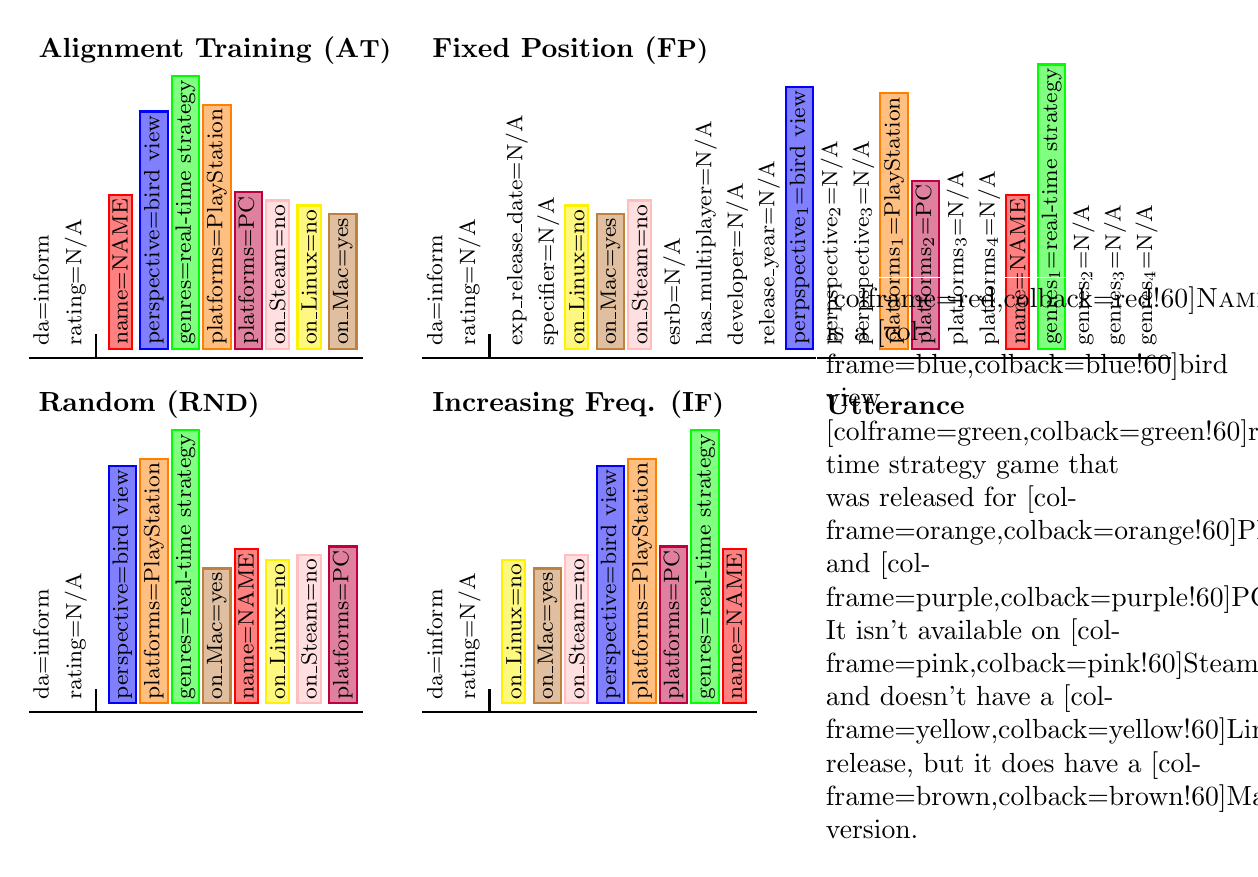
\begin{tikzpicture}[]


    \node[anchor=west] at (5.0,5.8) 
        {\textbf{Fixed Position \textsc{(F\small{P})}}};
    \node[anchor=west] at (0.0,5.8) 
        {\textbf{Alignment Training \textsc{(A\small{T})}}};
    \draw[thick] (0.85,1.9) -- (0.85,2.2);
    \draw[thick] (0,1.9) -- (4.25,1.9);
    \draw[thick] (5 + 0.85,1.9) -- (5 + 0.85,2.2);
    \draw[thick] (5 + 0,1.9) -- (10.25+ 4.25,1.9);
    \draw[thick] (0.85,-2.6) -- (0.85,-2.3);
    \draw[thick] (0,-2.6) -- (4.25,-2.6);
    \draw[thick] (5+0.85,-2.6) -- (5+0.85,-2.3);
    \draw[thick] (5+0,-2.6) -- (5+4.25,-2.6);

    \node[anchor=north west,inner sep=0.5mm,rotate=90] at (0,2) 
        {\footnotesize da=inform};
    \node[anchor=north west,inner sep=0.5mm,rotate=90] at (0.4,2) 
        {\footnotesize rating=N/A};
    \node[anchor=north west,rotate=90,inner sep=0.5mm,draw=red,thick,fill=red!50] 
        at (0.2 + 0.8,2) 
        {\footnotesize name=NAME};
    \node[anchor=north west,rotate=90,inner sep=0.5mm,draw=blue,thick,fill=blue!50] 
        at (0.2 + 1.2,2) {\footnotesize perspective=bird view};
    \node[anchor=north west,rotate=90,inner sep=0.5mm,draw=green,thick,
          fill=green!50] 
        at (0.2 + 1.6,2) {\footnotesize genres=real-time strategy};
    \node[anchor=north west,rotate=90,inner sep=0.5mm,draw=orange,thick,
          fill=orange!50] 
        at (0.2 + 2.0,2) {\footnotesize platforms=PlayStation};
    \node[anchor=north west,rotate=90,inner sep=0.5mm,draw=purple,thick,
          fill=purple!50] 
        at (0.2 + 2.4,2) {\footnotesize platforms=PC};
    \node[anchor=north west,rotate=90,inner sep=0.5mm,draw=pink,thick,
          fill=pink!50] 
        at (0.2 + 2.8,2) {\footnotesize on\_Steam=no};
    \node[anchor=north west,rotate=90,inner sep=0.5mm,draw=yellow,thick,
          fill=yellow!50] 
        at (0.2 + 3.2,2) {\footnotesize on\_Linux=no};
    \node[anchor=north west,rotate=90,inner sep=0.5mm,draw=brown,thick,
          fill=brown!50] 
        at (0.2 + 3.6,2) {\footnotesize on\_Mac=yes};


\node[anchor=north west,inner sep=0.5mm,rotate=90] at (5 + 0,2) 
    {\footnotesize da=inform};
\node[anchor=north west,inner sep=0.5mm,rotate=90] at (5 + 0.4,2) 
    {\footnotesize rating=N/A};
\node[anchor=north west,rotate=90,inner sep=0.5mm] 
    at (5.2 + 0.8,2) 
    {\footnotesize exp\_release\_date=N/A};
\node[anchor=north west,rotate=90,inner sep=0.5mm] 
    at (5.2 + 1.2,2) 
    {\footnotesize specifier=N/A};
\node[anchor=north west,rotate=90,inner sep=0.5mm,draw=yellow,thick,fill=yellow!50] 
    at (5.2 + 1.6,2) 
    {\footnotesize on\_Linux=no};
\node[anchor=north west,rotate=90,inner sep=0.5mm,draw=brown,thick,fill=brown!50] 
    at (5.2 + 2.0,2) 
    {\footnotesize on\_Mac=yes};
\node[anchor=north west,rotate=90,inner sep=0.5mm,draw=pink,thick,fill=pink!50] 
    at (5.2 + 2.4,2) 
    {\footnotesize on\_Steam=no};
\node[anchor=north west,rotate=90,inner sep=0.5mm] 
    at (5.2 + 2.8,2) 
    {\footnotesize esrb=N/A};
\node[anchor=north west,rotate=90,inner sep=0.5mm] 
    at (5.2 + 3.2,2) 
    {\footnotesize has\_multiplayer=N/A};

   % ['inform', 'rating=N/A', 'exp_release_date=N/A', 'specifier=N/A', 'has_linux_release=no', 'has_mac_release=yes', 'available_on_steam=no', 'esrb=N/A', 'has_multiplayer=N/A', 'developer=N/A', 'release_year=N/A', 'player_perspective=bird view', 'player_perspective=N/A', 'player_perspective=N/A', 'platforms=PlayStation', 'platforms=PC', 'platforms=N/A', 'platforms=N/A', 'name=PLACEHOLDER', 'genres=real-time strategy', 'genres=N/A', 'genres=N/A', 'genres=N/A']
\node[anchor=north west,rotate=90,inner sep=0.5mm] 
    at (5.2 + 3.6,2) 
    {\footnotesize developer=N/A};
\node[anchor=north west,rotate=90,inner sep=0.5mm] 
    at (5.2 + 4.0,2) 
    {\footnotesize release\_year=N/A};
\node[anchor=north west,rotate=90,inner sep=0.5mm,draw=blue,thick,fill=blue!50] 
    at (5.2 + 4.4,2) 
    {\footnotesize perpspective\textsubscript{1}=bird view};
\node[anchor=north west,rotate=90,inner sep=0.5mm] 
    at (5.2 + 4.8,2) 
    {\footnotesize perpspective\textsubscript{2}=N/A};
\node[anchor=north west,rotate=90,inner sep=0.5mm] 
    at (5.2 + 5.2,2) 
    {\footnotesize perpspective\textsubscript{3}=N/A};
\node[anchor=north west,rotate=90,inner sep=0.5mm,draw=orange,thick,fill=orange!50] 
    at (5.2 + 5.6,2) 
    {\footnotesize platforms\textsubscript{1}=PlayStation};
\node[anchor=north west,rotate=90,inner sep=0.5mm,draw=purple,thick,fill=purple!50] 
    at (5.2 + 6.0,2) 
    {\footnotesize platforms\textsubscript{2}=PC};
\node[anchor=north west,rotate=90,inner sep=0.5mm] 
    at (5.2 + 6.4,2) 
    {\footnotesize platforms\textsubscript{3}=N/A};
\node[anchor=north west,rotate=90,inner sep=0.5mm] 
    at (5.2 + 6.8,2) 
    {\footnotesize platforms\textsubscript{4}=N/A};
\node[anchor=north west,rotate=90,inner sep=0.5mm,draw=red,thick,fill=red!50] 
    at (5.2 + 7.2,2) 
    {\footnotesize name=NAME};
\node[anchor=north west,rotate=90,inner sep=0.5mm,draw=green,thick,fill=green!50] 
    at (5.2 + 7.6,2) 
    {\footnotesize genres\textsubscript{1}=real-time strategy};
\node[anchor=north west,rotate=90,inner sep=0.5mm] 
    at (5.2 + 8.0,2) 
    {\footnotesize genres\textsubscript{2}=N/A};
\node[anchor=north west,rotate=90,inner sep=0.5mm] 
    at (5.2 + 8.4,2) 
    {\footnotesize genres\textsubscript{3}=N/A};
\node[anchor=north west,rotate=90,inner sep=0.5mm] 
    at (5.2 + 8.8,2) 
    {\footnotesize genres\textsubscript{4}=N/A};


%\node[anchor=north west,rotate=90] at (1.5,2) {genres=platformer};
%\node[anchor=north west,rotate=90] at (2,2) {genres=puzzle};
%\node[anchor=north west,rotate=90] at (2.5,2) {perspective=side vew};
%\node[anchor=north west,rotate=90] at (3,2) {name=NAME};
%\node[anchor=north west,rotate=90] at (3.5,2) {name=NAME};
%\node[anchor=north west,rotate=90] at (4,2) {name=NAME};
%\node[anchor=north west,rotate=90] at (4.5,2) {name=NAME};
%
%
%\node[anchor=north west,rotate=90] at (5.5+0,2) {\small give opinion};
%\node[anchor=north west,rotate=90] at (5.5+0.5,2) {\small rating=good};
%\node[anchor=north west,rotate=90] at (5.5+1,2) {\small genres=adventure};
%\node[anchor=north west,rotate=90] at (5.5+1.5,2) {genres=platformer};
%\node[anchor=north west,rotate=90] at (5.5+2,2) {genres=puzzle};
%\node[anchor=north west,rotate=90] at (5.5+2.5,2) {perspective=side vew};
%\node[anchor=north west,rotate=90] at (5.5+3,2) {name=NAME};
%\node[anchor=north west,rotate=90] at (5.5+3.5,2) {name=NAME};
%\node[anchor=north west,rotate=90] at (5.5+4,2) {name=NAME};
%\node[anchor=north west,rotate=90] at (10+0,2) {give opinion};
%\node[anchor=north west,rotate=90] at (10+0.5,2) {rating=good};
%\node[anchor=north west,rotate=90] at (10+1,2) {genres=adventure};
%\node[anchor=north west,rotate=90] at (10+1.5,2) {genres=platformer};
%\node[anchor=north west,rotate=90] at (10+2,2) {genres=puzzle};
%\node[anchor=north west,rotate=90] at (10+2.5,2) {perspective=side vew};
%\node[anchor=north west,rotate=90] at (10+3,2) {name=NAME};
%\node[anchor=north west,rotate=90] at (10+3.5,2) {name=NAME};
%\node[anchor=north west,rotate=90] at (10+4,2) {name=NAME};
%\node[anchor=north west,rotate=90] at (10+4.5,2) {name=NAME};
%
%



%['give_opinion', 'rating=good', 'genres=adventure', 'genres=platformer', 'genres=puzzle', 'player_perspective=side view', 'name=PLACEHOLDER']


%#
%#

%['inform', 'rating=N/A', 'exp_release_date=N/A', 'specifier=N/A', 'has_linux_release=no', 'has_mac_release=yes', 'available_on_steam=no', 'esrb=N/A', 'has_multiplayer=N/A', 'developer=N/A', 'release_year=N/A', 'player_perspective=bird view', 'player_perspective=N/A', 'player_perspective=N/A', 'platforms=PlayStation', 'platforms=PC', 'platforms=N/A', 'platforms=N/A', 'name=PLACEHOLDER', 'genres=real-time strategy', 'genres=N/A', 'genres=N/A', 'genres=N/A']


%inc_freq_delex
%['inform', 'rating=N/A', 'has_linux_release=no', 'has_mac_release=yes', 'available_on_steam=no', 'player_perspective=bird view', 'platforms=PlayStation', 'platforms=PC', 'name=PLACEHOLDER', 'genres=real-time strategy']

\node[anchor=north west,inner sep=0.5mm,rotate=90] at (0,-2.5) 
    {\footnotesize da=inform};
\node[anchor=north west,inner sep=0.5mm,rotate=90] at (0.4,-2.5) 
    {\footnotesize rating=N/A};
\node[anchor=north west,rotate=90,inner sep=0.5mm,draw=blue,thick,fill=blue!50] 
    at (0.2 + 0.8,-2.5) 
    {\footnotesize perspective=bird view};

\node[anchor=north west,rotate=90,inner sep=0.5mm,draw=orange,thick,fill=orange!50] 
    at (0.2 + 1.2,-2.5) 
    {\footnotesize platforms=PlayStation};
\node[anchor=north west,rotate=90,inner sep=0.5mm,draw=green,thick,fill=green!50] 
    at (0.2 + 1.6,-2.5) 
    {\footnotesize genres=real-time strategy};


\node[anchor=north west,rotate=90,inner sep=0.5mm,draw=brown,thick,fill=brown!50] 
    at (0.2 + 2.0,-2.5) 
    {\footnotesize on\_Mac=yes};
\node[anchor=north west,rotate=90,inner sep=0.5mm,draw=red,thick,fill=red!50] 
    at (0.2 + 2.4,-2.5) 
    {\footnotesize name=NAME};

\node[anchor=north west,rotate=90,inner sep=0.5mm,draw=yellow,thick,fill=yellow!50] 
    at (0.2 + 2.8,-2.5) 
    {\footnotesize on\_Linux=no};
\node[anchor=north west,rotate=90,inner sep=0.5mm,draw=pink,thick,fill=pink!50] 
    at (0.2 + 3.2,-2.5) 
    {\footnotesize on\_Steam=no};
\node[anchor=north west,rotate=90,inner sep=0.5mm,draw=purple,thick,fill=purple!50] 
    at (0.2 + 3.6,-2.5) 
    {\footnotesize platforms=PC};

    \node[anchor=west] at (0,1.3) {\textbf{Random \textsc{(R\small{ND})}}};



\node[anchor=north west,inner sep=0.5mm,rotate=90] at (5 + 0,-2.5) 
    {\footnotesize da=inform};
\node[anchor=north west,inner sep=0.5mm,rotate=90] at (5 + 0.4,-2.5) 
    {\footnotesize rating=N/A};
\node[anchor=north west,rotate=90,inner sep=0.5mm,draw=yellow,thick,fill=yellow!50] 
    at (5.2 + 0.8,-2.5) 
    {\footnotesize on\_Linux=no};
\node[anchor=north west,rotate=90,inner sep=0.5mm,draw=brown,thick,fill=brown!50] 
    at (5.2 + 1.2,-2.5) 
    {\footnotesize on\_Mac=yes};
\node[anchor=north west,rotate=90,inner sep=0.5mm,draw=pink,thick,fill=pink!50] 
    at (5.2 + 1.6,-2.5) 
    {\footnotesize on\_Steam=no};

\node[anchor=north west,rotate=90,inner sep=0.5mm,draw=blue,thick,fill=blue!50]
    at (5.2 + 2.0,-2.5) 
    {\footnotesize perspective=bird view};
\node[anchor=north west,rotate=90,inner sep=0.5mm,draw=orange,thick,fill=orange!50] 
    at (5.2 + 2.4,-2.5) 
    {\footnotesize platforms=PlayStation};
\node[anchor=north west,rotate=90,inner sep=0.5mm,draw=purple,thick,fill=purple!50] 
    at (5.2 + 2.8,-2.5) 
    {\footnotesize platforms=PC};

\node[anchor=north west,rotate=90,inner sep=0.5mm,draw=green,thick,fill=green!50] 
    at (5.2 + 3.2,-2.5) 
    {\footnotesize genres=real-time strategy};
\node[anchor=north west,rotate=90,inner sep=0.5mm,draw=red,thick,fill=red!50] 
    at (5.2 + 3.6,-2.5) 
    {\footnotesize name=NAME};
%has_linux_release=no', 'has_mac_release=yes', 'available_on_steam=no', 'player_perspective=bird view', 'platforms=PlayStation', 'platforms=PC', 'name=PLACEHOLDER', 'genres=real-time strategy'
    \node[anchor=west] at (5.0,1.3) {\textbf{Increasing Freq. \textsc{(I\small{F})}}};


%\node[anchor=north west,inner sep=0.5mm,rotate=90] at (10 + 0,-2.5) 
%    {\footnotesize da=inform};
%\node[anchor=north west,inner sep=0.5mm,rotate=90] at (10 + 0.4,-2.5) 
%    {\footnotesize rating=N/A};
%
%\node[anchor=north west,rotate=90,inner sep=0.5mm,draw=red,thick,fill=red!50] 
%    at (10.2 + 0.8,-2.5) 
%    {\footnotesize name=NAME};
%
%\node[anchor=north west,rotate=90,inner sep=0.5mm,draw=green,thick,fill=green!50] 
%    at (10.2 + 1.2,-2.5) 
%    {\footnotesize genres=real-time strategy};
%
%    \node[anchor=north west,rotate=90,inner sep=0.5mm,draw=purple,thick,fill=purple!50] 
%    at (10.2 + 1.6,-2.5) 
%    {\footnotesize platforms=PC};
%\node[anchor=north west,rotate=90,inner sep=0.5mm,draw=orange,thick,fill=orange!50] 
%    at (10.2 + 2.0,-2.5) 
%    {\footnotesize platforms=PlayStation};
%
%\node[anchor=north west,rotate=90,inner sep=0.5mm,draw=blue,thick,fill=blue!50]
%    at (10.2 + 2.4,-2.5) 
%    {\footnotesize perspective=bird view};
%\node[anchor=north west,rotate=90,inner sep=0.5mm,draw=pink,thick,fill=pink!50] 
%    at (10.2 + 2.8,-2.5) 
%    {\footnotesize on\_Steam=no};
%\node[anchor=north west,rotate=90,inner sep=0.5mm,draw=brown,thick,fill=brown!50] 
%    at (10.2 + 3.2,-2.5) 
%    {\footnotesize on\_Mac=yes};
%\node[anchor=north west,rotate=90,inner sep=0.5mm,draw=yellow,thick,fill=yellow!50] 
%    at (10.2 + 3.6,-2.5) 
%    {\footnotesize on\_Linux=no};
%




%has_linux_release=no', 'has_mac_release=yes', 'available_on_steam=no', 'player_perspective=bird view', 'platforms=PlayStation', 'platforms=PC', 'name=PLACEHOLDER', 'genres=real-time strategy'
%    \node[anchor=west] at (10.0,1.3) {\textbf{Decreasing Freq.}};




    \node[anchor=west] at (10, 1.3) {\textbf{Utterance}};
\node[text width=5.0cm,draw=white,anchor=west] at (10,-0.7) {
    {\mybox[colframe=red,colback=red!60]{\textsc{Name}}} is a 
    \mybox[colframe=blue,colback=blue!60]{bird view} 
    \mybox[colframe=green,colback=green!60]{real-time strategy} 
    game that was released for 
    \mybox[colframe=orange,colback=orange!60]{PlayStation} and 
    \mybox[colframe=purple,colback=purple!60]{PC.} It isn't available on 
    \mybox[colframe=pink,colback=pink!60]{Steam} and doesn't have a 
    \mybox[colframe=yellow,colback=yellow!60]{Linux} release, but it does have
    a \mybox[colframe=brown,colback=brown!60]{Mac} version.
};


\end{tikzpicture}

\caption{Example \meaningrepresentation~linearization strategies for an utterance (lower right) from the 
    ViGGO training set.}
\label{fig:linstrats}
\end{figure}


\paragraph{Increasing Frequency (\textsc{If})} 
In the \textsc{Increasing Frequency} linearization (\textsc{If}), 
we order the attribute-value pairs by increasing frequency of 
occurrence in the training data
i.e. $\acount(\attr_i=\aval_i) \le \acount(\attr_{i+1}=\aval_{i+1})$.
We hypothesize that placing frequently occurring items in a consistent location
may make it easier for the generation model to realize those items correctly, possibly
at the expense of rarer items.

\paragraph{Fixed Position (\textsc{Fp})} We take  consistency one step further 
and create a fixed ordering of all attributes, \textit{n.b.} not attribute-values, ordering them in increasing
frequency of occurrence on the training set (i.e. every instance has the same
order of attributes in the encoder input). In this \textsc{Fixed Position}
linearization (\textsc{Fp}), attributes that are not present 
in an \meaningrepresentation~are explicitly represented with an \textit{N/A} value. 
For list-valued slots, we determine the maximum length list in the training
data and create that many repeated slots in the input sequence.
This linearization is feasible for datasets with a modest number of 
unique attributes (in our case ViGGO has 14 attributes and
the E2E Challenge corpus has eight) but would not easily scale to 10s, 100s, or larger
attribute vocabularies. 






\subsection{Phrase-based Data Augmentation}

\begin{figure}
    \centering


        \begin{tikzpicture}

            \def\th{5mm};
            \def\td{2mm};
    \node[text height=\th,text depth=\td] (aromi) at (-5,-4) {Aromi};
            \node[text height=\th,text depth=\td] (is) at (-1.5,-4) {is};
            \node[text height=\th,text depth=\td] (not) at (0.0,-4) {not};

            \node[text height=\th,text depth=\td] (a) at (1.5,-4) {a};
            \node[text height=\th,text depth=\td] (ff) at (4,-4) {family-friendly};
            \node[text height=\th,text depth=\td] (est) at (6.5,-4) {establishment};


            \node (root) at (-2.5,0) {S};
            \node[draw,circle,font=\small,inner sep=0] at ($(root)+(-0.5,0.5)$) {4};
            \node (rootNP) at (-5,-1) {NP};
            \node[draw,circle,font=\small,inner sep=0] at ($(rootNP)+(-0.5,0.5)$) {3};
            \node (rootNPNNP) at (-5,-2) {NNP};
            \node (r1c2) at (0.0,-1) {VP};
            \node[draw,circle,font=\small,inner sep=0] at ($(r1c2)+(0.5,0.5)$) {2};
                \node (r2c3) at (4,-2) {NP};
            \node[draw,circle,font=\small,inner sep=0] at ($(r2c3)+(0.5,0.5)$) {1};
                \node (det) at (1.5,-3) {DET};
                \node (jj) at (4,-3) {JJ};
                \node (nn) at (6.5,-3) {NN};
                \node (r2c1) at (-1.5,-2) {VB};

                \node (r2c2) at (0.0,-2) {RB};
                \draw[-] (r1c2) -- (r2c1);
                \draw[-] (r1c2) -- (r2c2);
                \draw[-] (r1c2) -- (r2c3);


                \draw[-] (r2c1) -- (is);

            \draw[-] (rootNPNNP) -- (aromi);
            \draw[-] (root.south west) -- (rootNP.north east);
            \draw[-] (rootNP) -- (rootNPNNP);
            \draw[-] (root.south east) -- (r1c2.north west);
                \draw[-] (r2c3) -- (det);
                \draw[-] (r2c3) -- (jj);
                \draw[-] (r2c3) -- (nn);
                \draw[-] (det) -- (a);
                \draw[-] (jj) -- (ff);
                \draw[-] (nn) -- (est);
                \draw[-] (r2c2) -- (not);
        

      %      \node[anchor=north west,align=left,inner sep=0,outer sep=0,text height=0mm,text width=11cm] at (0.7,0.5) {
                    %\begin{enumerate}
                    %    \item Parse training examples.
                %\item<3-> Create additional training examples from constituent phrases.
                %\end{enumerate}};

        \end{tikzpicture}

        ~\\~\\

        \begin{tabular}{ccc}
            \toprule
            &         \MeaningRepresentation~($\mr$) & Utterance ($\utttoks$) \\
            \midrule
            \raisebox{0.5pt}{\textcircled{\raisebox{-0.9pt} {1}}} &  
        $\left[\!\!\left[ \begin{array}{l} 
            \textsc{Inform}\\ 
            \AV{family\_friendly}{yes} 
        \end{array}   \right]\!\!\right]$  & 
            $\left[\textit{<<s>>}, \textit{a}, \textit{family-friendly}, \textit{establishment}, \textit{<<e>>}\right]$\\
        \raisebox{0.5pt}{\textcircled{\raisebox{-0.9pt} {2}}} &
        $\left[\!\!\left[ \begin{array}{l} 
            \textsc{Inform}\\ 
            \AV{family\_friendly}{no} 
        \end{array}\right]\!\!\right]$  & 
            $\left[\textit{<<s>>}, \textit{is}, \textit{not}, \textit{a}, 
            \textit{family-friendly}, \textit{establishment}, \textit{<<e>>}\right]$ \\
        \raisebox{0.5pt}{\textcircled{\raisebox{-0.9pt} {3}}} &
        $\left[\!\!\left[ \begin{array}{l} 
            \textsc{Inform}\\ 
            \AV{name}{Aromi} \end{array}   
        \right]\!\!\right]$ &  
        $\left[\textit{<<s>>}, \textit{aromi}, \textit{<<e>>}\right]$ \\
        \raisebox{0.5pt}{\textcircled{\raisebox{-0.9pt} {4}}} &
        $\left[\!\!\left[ \begin{array}{l}
            \textsc{Inform}\\ 
            \AV{name}{Aromi} \\ 
            \AV{family\_friendly}{no} 
        \end{array}\right]\!\!\right]$  & 
        $\left[\textit{<<s>>}, \textit{aromi}, \textit{is}, \textit{not}, 
               \textit{a}, \textit{family-friendly}, \textit{establishment}, 
               \textit{<<e>>}\right]$ \\
        \bottomrule
        \end{tabular}
    \caption{Example training instances produced from the phrase-based
            data augmentation protocol. The constituent parse is shown
        above. Numbered phrase nodes correspond to the phrase examples
    created in the table below.}
            \label{fig:pbdaexample}
\end{figure}


While the alignment training linearization leads to a controllable model,
there is evidence that sequence-to-sequence models do not behave very
systemically with standard training methods 
\cite{lake2018generalization,loula2018rearranging}. By systematic, we mean that
$h = enc_\theta(\ls(\mr))$ is highly training data dependent and 
 small changes in $\ls(\mr)$ may lead to large, non-linear
changes in h, and as a consequence, the decoder may succeed on
on one $\ls(\mr)$ but fail on another $\ls^\prime(\mr)$ even when the 
differences between the permutations are small. With this in mind, we propose
two data augmentations to make explicit examples of  modular pairwise 
transitions and constituent structure reuse so that models trained with alignment training
may systemically recombine these elements to generate any ordering.
See \autoref{tab:augdat} for statistics of the generated training data.


We augment the training data with MR/utterance pairs taken from constituent
phrases in the original training data. 
We parse all training utterances and enumerate all constituent phrases
governed by 
NP, VP, ADJP, ADVP, PP, S, Sbar
non-terminals.\footnote{We used the \href{https://stanfordnlp.github.io/CoreNLP/}{Stanford CoreNLP parser v3.9.2}.} We then apply the attribute-value 
matching rules
used for alignment training (see \autoref{sec:align})
to obtain a corresponding MR, keeping the dialog act 
of the original utterance. We discard
phrases with no realized attributes.
See \autoref{tab:main.dataset.stats} for augmented data statistics.

Because 
we reclassify the MR of phrases using the matching rules, 
the augmented  data includes examples of
how to invert binary attributes, e.g. from the phrase
``is not on Mac,'' which implies \AV{has\_mac\_release}{no},
we obtain the phrase ``on Mac'' which implies 
\AV{has\_mac\_release}{yes}.
When presenting the linearized MR of phrase examples to the model encoder
we prepend and append phrase specific \textit{start} and \textit{stop} tokens respectively
(e.g., \textit{start-NP} and \textit{stop-NP}) to prevent the model
from ever producing an incomplete sentence when generating for a complete MR.




\subsection{Datasets}

We run our alignment training experiments on the E2E Challenge dataset as well
 as the more recently released 
 ViGGO corpus \citep{juraska2019} another English language, task-oriented dialogue
dataset.\footnote{\url{https://nlds.soe.ucsc.edu/viggo}}
The ViGGO corpus comes from the video game domain (e.g. conversations with
a video game recommendation agent)  and  contains 14 attribute types
and nine dialogue acts. %(\DA{Request Explanation}, \DA{Recommend}, etc.).  
In
addition to binary and categorical valued attributes, the corpus also features
list-valued attributes which can have a variable number of values, and an
open-class \Atr{specifier} attribute. 



%?% the \href{http://www.macs.hw.ac.uk/InteractionLab/E2E/}{E2E
%?%Challenge} corpus \cite{novikova2017} and the
%?The ViGGO dataset comes from the video game domain.
%? %These
%?datasets provide MR/utterance pairs from the restaurant and video game
%?domains, respectively. Examples from the E2E corpus (33,523 train/1,426
%?dev/630 test) can have up to eight unique attributes.  There is only one
%?dialogue act for the corpus, \textsc{Inform}.  Attribute-values are either binary
%?or categorical valued.

\subsubsection{MR/Utterance Alignments} \label{sec:align}

The original datasets do not have alignments between individual
attribute-value pairs and the subsequences of the utterances they occur in, 
which we
need for the alignment training linearization strategy.  We manually developed a
list of heuristic pattern matching rules (e.g. \textit{not kid-friendly}
$\rightarrow$ \AV{family\_friendly}{no}) which we use to tag the utterance
tokens.  For ViGGO, we started from scratch,
but for the E2E Challenge dataset we greatly expanded the rule-set created by \citet{dusek2019}.  To
ensure the correctness of the rules, we iteratively added new matching rules,
ran them on the training and validation sets, and verified that they produced
the same \meaningrepresentation~as was provided in the dataset. This process took the author
roughly two weeks to produce approximately 25,000 and 1,500 rules for the E2E
and ViGGO datasets respectively. Note that the large number of rules is
obtained programmatically, i.e. creating template rules and inserting matching
keywords or phrases (e.g., enumerating variants such as \textit{not
kid-friendly}, \textit{not child-friendly}, \textit{not family-friendly}, etc.).


\begin{table}
\centering
\begin{tabular}{cc cccc}
\toprule
Dataset & Train & Augmented & Valid & Test \\
\midrule
E2E Challenge & 33,523 & 443,192 & & \\
ViGGO         &  5,103 &  67,445 &  & \\
% contains 5,103 train/246 dev/359 test)
\bottomrule
\end{tabular}
\caption{Dataset sizes (including data augmentation) after correcting
the training and validation instances.}
\label{tab:cgdata}
\end{table}


In cases where the matching rules produced different \meaningrepresentations~than provided in the
original dataset, we manually checked them. If the rule was incorrect,
we added a new rule to account for the exception. 
In many cases in the E2E Challenge
dataset
and several times in the ViGGO corpus, we found the rule to be correct and the \meaningrepresentation~to be
incorrect for the given utterance. In those cases, we used the corrected \meaningrepresentations~for
training and validation. %To maintain comparability to prior work, 
We
do not modify the test sets in any way. We follow \citet{dusek2019} and remove from the training and validation
sets any modified exampels that share a \meaningrepresentation~also
found in the test set. This creates slightly different training and validation
set numbers for the E2E Challenge
dataset than in the faithful generation experiments. See \autoref{tab:cgdata} for 
statistics.
We use the matching rules to develop  a rule-based utterance 
tagger to implement the alignment training linearization, phrase-based data augmentation
protocol, and as a reranker when generating utterances in our experiments.
%, we can
%determine alignments between the provided \meaningrepresentation~and the realized utterances.





For most cases, the attribute-values uniquely correspond to a non-overlapping
subsequences of the utterance. The \Atr{rating} attribute in the ViGGO dataset,
however, could have multiple reasonable mappings to the utterance, so we treat
it in practice like an addendum to the dialogue act, occurring directly after the
dialogue act as part of a ``header'' section in any \meaningrepresentation~linearization strategy
(see \autoref{fig:linstrats} where \AV{rating}{N/A} occurs after the dialogue
act regardless of choice of linearization strategy).

\paragraph{Delexicalization} The ViGGO corpus is relatively small and the
attributes \Atr{name}, \Atr{developer}, \Atr{release\_year},
\Atr{expected\_release\_date}, and \Atr{specifier}~can have values that are
only seen several times during training. Neural models often struggle to learn
good representations for infrequent inputs, which can, in turn, lead to poor
test-set generalization. To alleviate this, we delexicalize these values in
the utterance. That is, we replace them with an attribute specific placeholder
token.

\label{app:specifier} Additionally, for \Atr{specifier} whose values come from the open class of
adjectives, we represent the specified adjective with a placeholder which
marks two features, whether it is consonant (C) or vowel initial (V) (e.g.
``\uline{d}ull'' vs. ``\uline{o}ld'') and whether it is in regular (R) or
superlative (S) form (e.g. ``dull'' vs. ``dullest'') since these features can
effect the surrounding context in which the adjective is realized.  See the
following lexicalized/delexicalized examples:
\begin{itemize}
        \item \AV{specifier}{oldest}~-- vowel initial, superlative
\begin{itemize}
    \item \textit{What is the oldest game you've played?}
    \item \textit{What is the SPECIFIER\_V\_S game you've played?}
\end{itemize}
        \item \AV{specifier}{old}~-- vowel initial, regular

\begin{itemize}
    \item \textit{What is an old game you've played?}
    \item \textit{What is an SPECIFIER\_V\_R game you've played?}
\end{itemize}

        \item \AV{specifier}{new}~-- consonant initial, regular

\begin{itemize}
    \item \textit{What is a new game you've played?}
    \item \textit{What is a SPECIFIER\_C\_R game you've played?}
\end{itemize}
\end{itemize}

All generated delexicalized utterances are post-processed with the
corresponding attribute-values before computing evaluation metrics (i.e., 
they are re-lexicalized with the appropriate value strings from the input \meaningrepresentation). Unlike in the faithful generation experiments, we 
do not perform any delexicalization of the E2E Challenge corpus.








\subsection{Generation Models}
We examine the effects of linearization strategy and data augmentation
on biGRU (see \autoref{sec:nlggru})
and transformer (see \autoref{sec:nlgtf}) based \sequencetosequence~models.
See \autoref{tab:nlghpsspace} for the set of hyper-parameters that we explored for
each model and \autoref{tab:gruparams} and \autoref{tab:tfparams} for the winning hyper-parameter settings for the biGRU and transformer models respectively.
Hyper-parameters were found using grid-search, selecting the model
with best validation \textsc{Bleu} score. We performed a separate
grid-search for each architecture-linearization strategy pairing in case
there was no one best hyper-parameter setting.
We used a batch size of 128 for all biGRU and
Transformer models and trained for at most 700 epochs.



\begin{table}
    \centering
    \begin{tabular}{cp{4.25cm}p{4.25cm}}
            \toprule
            Hyperparameter & biGRU & Transformer\\
            \midrule
            Layers & $1$, $2$ & $1$, $2$\\
            Label Smoothing & $0.0$, $0.1$ & $0.0$, $0.1$\\
            Weight Decay & $0$, $10^-5$ & --- \\
Optimizer/Learning Rate & Adam/$10^{-3}$, Adam/$10^{-4}$, Adam/$10^{-5}$,
            SGD/$0.5$, SGD/$0.25$, SGD/$0.1$ & Adam with the learning
            rate schedule from \cite{rush2018} (factor=1, warmup=8000)\\
        Tied Decoder Embeddings & tied, untied & tied, untied\\
        Attention & Bahdanau, General & ---\\
        \bottomrule
\end{tabular}
\caption{Hyperparameter search space for biGRU and transformer architectures.}
\label{tab:nlghpsspace}
\end{table}


\begin{table}
\small
\center
\begin{tabular}{clccc ccc cc ccccc}
\toprule
&Model & L & LS & WD & Optim. & LR & Attn & $\embDim$ & $\hidDim$ & $\encDim$ & $\decDim$ & Drop. & Params \\
\midrule
    \parbox[t]{2mm}{\multirow{6}{*}{\rotatebox[origin=c]{90}{E2E}}} 
 & \textsc{Rnd} & 2 & 0.1 & $10^{-5}$ & Adam & $10^{-5}$ &  Bahd. & 512 & 512 & 1024 & 512 & 0.1 & 14,820,419  \\
 & \textsc{Fp} & 2 & 0.1 & $10^{-5}$ & SGD & $0.1$ &  Bahd. & 512 & 512 & 1024 & 512 & 0.1 & 14,820,003 \\ 
 & \textsc{If} & 2 & 0.1 & $0.0$ & SGD & $0.5$ &  Gen. & 512 & 512 & 1024 & 512  & 0.1 & 14,557,763 \\
 & \textsc{If+p} & 2 & 0.1 & $0.0$ & SGD & $0.5$ &  Gen. &512 & 512 & 1024 & 512  & 0.1 &14,557,763 \\
 & \textsc{At} & 2 & 0.1 & $10^{-5}$ & Adam & $10^{-5}$ &  Bahd. & 512 & 512 & 1024 & 512  & 0.1 & 14,820,419  \\
 & \textsc{At+p} & 2 & 0.1 & $10^{-5}$ & Adam & $10^{-5}$ &  Bahd. & 512 & 512 & 1024 & 512  & 0.1 & 14,820,419  \\
\midrule
    \parbox[t]{2mm}{\multirow{6}{*}{\rotatebox[origin=c]{90}{ViGGO}}} 
 & \textsc{Rnd} & 2 & 0.1 & $10^{-5}$ & SGD & $0.25$ &  Gen. & 512 & 512 & 1024 & 512 & 0.1 & 14,274,865 \\
 & \textsc{Fp} & 1 & 0.1 & $10^{-5}$ & Adam & $10^{-5}$ &  Bahd. & 512 & 512 & 1024 & 512 & 0.1 & 7,718,193 \\ 
 & \textsc{If} & 1 & 0.0 & $0.0$ & SGD & $0.5$ &  Bahd. &  512 & 512 & 1024 & 512  & 0.1 & 7,712,049 \\ 
 & \textsc{If+} & 1 & 0.0 & $0.0$ & SGD & $0.5$ &  Bahd. & 512 & 512 & 1024 & 512  & 0.1 & 7,712,049 \\ 
 & \textsc{At} & 2 & 0.1 & $0.0$ & Adam & $10^{-5}$ &  Bahd. &  512 & 512 & 1024 & 512  & 0.1 & 14,537,521 \\ 
 & \textsc{At+p} & 2 & 0.1 & $0.0$ & Adam & $10^{-5}$ &  Bahd. &  512 & 512 & 1024 & 512  & 0.1 & 14,537,521 \\ 
\bottomrule
\end{tabular}

\caption{Winning hyperparameter settings for biGRU models. L, LS, and WD 
indicate number of layers, label smoothing, and weight decay respectively. 
All models use untied embeddings. Drop. indicates dropout (i.e. drop probability).}
\label{tab:gruparams}
\end{table}

\begin{table}
\center
\begin{tabular}{cl cccc ccccc}
\toprule
&Model & Layers & LS & Emb. & Params & $\embDim$ & $\hidDim$ & $\encDim$ & $\decDim$ & Dropout\\
\midrule
    \parbox[t]{2mm}{\multirow{6}{*}{\rotatebox[origin=c]{90}{E2E}}} 
 & \textsc{Rnd} & 1 & 0.1 & tied & 7,966,787 & 512 & 2048 & 512 & 512 & 0.1\\
 & \textsc{Fp} & 1 & 0.1 & tied & 7,970,371 & 512 & 2048 & 512 & 512 & 0.1\\
 & \textsc{If} & 1 & 0.1 & untied & 8,525,379 & 512 & 2048 & 512 & 512 & 0.1 \\
 & \textsc{If+p} & 1 & 0.1 & untied & 8,525,379 & 512 & 2048 & 512 & 512 & 0.1 \\
 & \textsc{At} & 2 & 0.1 & untied & 15,881,795 & 512 & 2048 & 512 & 512 & 0.1 \\
 & \textsc{At+p} & 2 & 0.1 & untied & 15,881,795 & 512 & 2048 & 512 & 512 & 0.1 \\
\midrule
    \parbox[t]{2mm}{\multirow{6}{*}{\rotatebox[origin=c]{90}{ViGGO}}} 
 & \textsc{Rnd} & 2 & 0.0 & untied & 15,598,897 & 512 & 2048 & 512 & 512 & 0.1\\
 & \textsc{Fp} & 2 & 0.1 & untied & 15,605,041 & 512 & 2048 & 512 & 512 & 0.1\\
 & \textsc{If} & 2 & 0.1 & untied & 15,598,897 & 512 & 2048 & 512 & 512 & 0.1 \\
 & \textsc{If+p} & 2 & 0.1 & untied & 15,598,897 & 512 & 2048 & 512 & 512 & 0.1\\
 & \textsc{At} & 2 & 0.1 & untied & 15,598,897 & 512 & 2048 & 512 & 512 & 0.1 \\
 & \textsc{At+p} & 2 & 0.1 & untied & 15,598,897 & 512 & 2048 & 512 & 512 & 0.1 \\
\bottomrule
\end{tabular}

\caption{Winning hyperparameter settings for transformer models 
(trained from scratch). L and  LS indicate number of layers and label smoothing respectively. Drop. indicates dropout (i.e. drop probability).
All models trained with the Adam optimizir with the learning
            rate schedule from \cite{rush2018} (factor=1, warmup=8000).
}
\label{tab:tfparams}
\end{table}

%lowest validation set cross-entropy. 
%
%\paragraph{Transformer}
%We used the Transformer S2S as implemented in
%\href{https://pytorch.org/}{PyTorch}.
%The input embedding dimension is 512 and inner hidden layer size is 2048.
%We used 8 heads in all multi-head attention layers.
%We used Sinusoidal position embeddings following those described in
%\citet{rush2018annotated}. Additionally, we used Adam with the learning
%rate schedule provided in that work (factor=1, warmup=8000).
%Dropout was set to 0.1.
%
%
\newcommand{\utt}{\ensuremath{\mathbf{y}}}
\newcommand{\uttVocab}{\ensuremath{\mathcal{W}}}
\newcommand{\da}{\ensuremath{a}}
\newcommand{\inseq}{\mathbf{x}}
\newcommand{\Attrs}{\ensuremath{\mathcal{V}}}
\newcommand{\inSize}{m}
\newcommand{\outSize}{n}

\newcommand{\mmhAttn}{\operatorname{maskedMHAttn}}
\newcommand{\mhAttn}{\operatorname{MHAttn}}

\newcommand{\mrEmb}{\mathbf{W}}
\newcommand{\uttEmb}{\mathbf{V}}
\newcommand{\decInput}{\mathbf{G}}
\newcommand{\decInputi}{\mathbf{g}_i}


\newcommand{\tfeA}{\boldsymbol{\check{\encInput}}^{(i)}}
\newcommand{\tfeB}{\boldsymbol{\bar{\encInput}}^{(i)}}
\newcommand{\tfeC}{\boldsymbol{\hat{\encInput}}^{(i)}}
\newcommand{\tfeD}{\boldsymbol{\dot{\encInput}}^{(i)}}
\newcommand{\tfeE}{\boldsymbol{\ddot{\encInput}}^{(i)}}

\newcommand{\tfdA}{\boldsymbol{\check{\decInput}}^{(i)}}
\newcommand{\tfdB}{\boldsymbol{\bar{\decInput}}^{(i)}}
\newcommand{\tfdC}{\boldsymbol{\hat{\decInput}}^{(i)}}
\newcommand{\tfdD}{\boldsymbol{\grave{\decInput}}^{(i)}}
\newcommand{\tfdE}{\boldsymbol{\tilde{\decInput}}^{(i)}}
\newcommand{\tfdF}{\boldsymbol{\acute{\decInput}}^{(i)}}
\newcommand{\tfdG}{\boldsymbol{\dot{\decInput}}^{(i)}}
\newcommand{\tfdH}{\boldsymbol{\ddot{\decInput}}^{(i)}}


%\subsection{Transformer Model Definition}
%
%Each Transformer layer is divided into blocks which each have three
%parts, (i) layer norm, (ii) feed-forward/attention, and  (iii) skip-connection.
%We first define the components used in the transformer blocks before
%describing the overall S2S transformer. 
%Starting with layer norm \cite{ba2016}, let $\encInput \in \reals^{m\times n}$, then we have
%$\layerNorm : \reals^{m \times n} \rightarrow \reals^{m \times n}$,
%\[\layerNorm(\encInput; \lnweightv, \lnbias) = \lnweight \odot (\encInput - \boldsymbol{\mu}) \odot \Lambda + \mathbf{b} \]
%
%where $\lnweightv, \lnbias \in \reals^n$ are learned parameters, $\odot$ is the elementwise product, $\lnweight = \left[\lnweightv,\ldots,\lnweightv\right] \in \reals^{m\times n}$ is a tiling of the parameter vector, $\lnweightv$, $m$ times, and  $\boldsymbol{\mu}, \boldsymbol{\Lambda} \in \reals^{m\times n}$ are
%defined elementwise as
%\[\boldsymbol{\mu}_{i,j} = \frac{1}{n} \sum_{k=1}^n \encInput_{i,k}\]
%and 
%\[\boldsymbol{\Lambda}_{i,j} = \left(
%    \sqrt{ \frac{1}{n-1} \sum_{k=1}^n \left( 
%\encInput_{i,k} - \boldsymbol{\mu}_{i,j} \right)^2  + \epsilon}\right)^{-1}\]
%respectively. The $\epsilon$ term is a small constant for numerical stability,
%set to $10^{-5}$.
%
%The inplace feed-forward layer, $\feedforward$, is a simple single-layer perceptron
%with $\relu$ activation 
%($\relu(\encInput) = \max\left(\zeroEmb, \encInput\right)$) \cite{nair2010}, applied to each row of an $m \times n$ input matrix, i.e. a sequence of $m$ objects
%with $n$ features,\\
%
%
%\noindent $\feedforward\left(\encInput;\weight{i},\weight{j},\bias{i},\bias{j}\right) =$
%\[  \relu\left(\encInput\weight{i} + \bias{i}\right)\weight{j} + \bias{j}     \]
%where $\weight{i} \in \reals^{\embDim \times \hidDim}$, $\bias{i} \in \reals^{\hidDim}$,
%$\weight{j} \in \reals^{\hidDim \times \embDim}$, $\bias{j} \in \reals^{\embDim}$ are learned parameters and 
%matrix-vector additions (i.e. $\mathbf{X} + \mathbf{b}$) are broadcast across
%the matrix rows.
%
%
%The final component to be defined is the multi-head attention, $\MultiAttn$ which is defined
%as\\
%
%\noindent  $\MultiAttn(\Query, \Key; \weight{a_1}, \weight{a_2}) =$
%\[ \left[ \begin{array}{c} 
%and $\bias{o} \in \reals^{\embDim}$ are learned parameters. 
%
%
%%We used the Transformer S2S as implemented in 
%%\href{https://pytorch.org/}{PyTorch}.
%The input embedding dimension is $\embDim= 512$ and inner hidden layer size 
%is $\hidDim=2048$. The encoder and decoder have separate parameters.
%We used $H=8$ heads in all multi-head attention layers. 
% We used Adam with the learning
%rate schedule provided in  \citet{rush2018} (factor=1, warmup=8000).
%Dropout was set to 0.1 was applied to input embeddings and each skip 
%connection (i.e. the third line in each block definition). As a 
%hyperparameter, we optionally tie the decoder input and output embeddings,
%i.e. $\decEmbs = \weight{o}$.

Additionally, we
fine-tune BART \cite{lewis2019bart}, a large pretrained transformer based 
\sequencetosequence~model. We stop fine-tuning after validation set cross-entropy stops decreasing.
We use the same settings as the fine-tuning for the CNN-DailyMail
summarization task,
although we modify the maximum number of updates to be roughly to be
equivalent to 10 epochs on the training set when using a 500 token batch
size, since
the number of updates effects
the learning rate scheduler. We selected the model iterate with
lowest validation set cross-entropy.

While BART is unlikely to have seen any linearized MR in its pretraining
data, its use of sub-word encoding  allows it to encode
arbitrary strings. Rather than extending it's encoder input vocabulary to
add the MR tokens, we simply format the input MR as a string
(in the correpsonding linearization order), e.g. ``inform rating=good name=NAME platforms=PC platforms=Xbox''.



\subsection{Utterance Planner Model} We experiment with three approaches to
creating a test-time utterance plan for the alignment training models. The
first is a bigram language model (\BgUP) over attribute-value sequences.
Attribute-value bigram counts are estimated from the training data 
(using Lidstone smoothing \citep{chen1996} with $\lidstone=10^{-6}$)  according to the
ordering determined by the matching rules (i.e. the alignment-training ordering). 

\begin{table}
\centering
\begin{tabular}{cc}
\toprule
Hyperparameter & Search Space\\
\midrule
Layers & 1, 2\\
Learning Rate &$10^{-3}$, $10^{-4}$, $10^{-5}$\\
RNN Cell & GRU, LSTM \\
Encoder direction & uni-, bi- \\
Label Smoothing & 0.0, 0.1\\
\bottomrule
\end{tabular}
\caption{Hyperparameter search space for the neural utterance planner (NUP).}
\label{tab:nuphps}
\end{table}


\begin{table}
\centering
\begin{tabular}{c ccc ccc ccccc}
\toprule
Dataset & L & Enc. Dir. & RNN Cell& LR & LS & Attn. &$\embDim$ & $\hidDim$  & $\encDim$ & $\decDim$ & Dropout \\
\midrule
   E2E & 1 & bi- &LSTM& $10^{-5}$ & 0.1 & Bahd. & 512 & 512 & 1024 & 512 &\\
   ViGGO & 1 & uni- & LSTM & $10^{-4}$ & 0.1 & Bahd.  & 512 & 512 & 1024 & 512 \\
\bottomrule
\end{tabular}
\caption{Winning hyperparameter options for the neural utterance planner (NUP)
model.}
\label{tab:nuphp}
\end{table}



The second model is a recurrent neural network based \sequencetosequence~model, which we refer to 
as the neural
utterance planner (\NUP). We train the \NUP~to map \textsc{If} ordered
attribute-values to the alignment training ordering. We grid-search model
hyperparameters, selecting the model with highest average Kendall's $\tau$
\citep{kendall1938} on the validation set alignment training orderings. See
\autoref{tab:nuphps} for the hyperparameter search space and \autoref{tab:nuphp} to see the chosen hyperameter setting. We used a batch size of 128, the Adam optimizer, and trained for at most 50 epochs.   Unlike the
\BgUP~model, the \NUP~model also conditions on the dialogue act, so it can
learn ordering preferences that differ across dialogue acts.

For both \BgUP~and \NUP, we use beam search (with beam size 32) to generate
candidate utterance plans. The beam search is constrained to only generate
attribute-value pairs that are given in the supplied \meaningrepresentation, and to avoid
generating repeated attributes. The search is not allowed to terminate until
all attribute-values in the \meaningrepresentation~are generated.  Beam candidates are ranked by
log likelihood. We show validation and test set Kendall's $\tau$ to the 
reference utterance for both planning models in \autoref{tab:uptau}.
A Kendall's $\tau$ of 1.0 indicates that the planner exactly follows the
human reference order while 0.0 indicates a random order relative to the
human reference. $\tau=-1$ indicates the model produces the reverse order
of the human reference plan. We see that the NUP produces utterance plans that are closer in order to the human reference on both the E2E Challenge and ViGGO datasets

\begin{table}
\centering

\begin{tabular}{ll c c}
\toprule
Dataset & Model & Valid & Test \\
\midrule
ViGGO & \textsc{BgUP} & 0.417 & 0.347 \\
                       & \textsc{NUP} & 0.739 & 0.651 \\
\midrule
E2E & \textsc{BgUP} & 0.433 & 0.432 \\
                       & \textsc{NUP} & 0.502 & 0.447 \\
\bottomrule
\end{tabular}


\caption{Validation and test set Kendall's $\tau$ for \textsc{BgUP} and 
NUP models.}
\label{tab:uptau}
\end{table}


The final ordering we propose is the \Oracle~ordering, i.e. the utterance plan
implied by the human-authored test-set reference utterances. This plan
represents the model performance if it had \textit{a priori}  knowledge of the
reference utterance plan. When a test example has multiple references, we
select the most frequent ordering in the references, breaking ties according
to \BgUP~log-likelihood.

\subsection{Experiments}

\subsubsection{Test-Set Evaluation}

In our first experiment, we compare performance of the proposed models and
linearization strategies on the E2E Challenge and ViGGO test sets. 
We refer to models using the alignment training linearization strategy
as \textsc{At+BgUP}, \textsc{At+NUP}, or \textsc{At+Oracle} depending
on whether the model is following the bigram planner, neural planner, or
human reference plan respectively.
For the \textsc{If}
and \textsc{At+NUP} models we also include variants trained on
the union of original training data and phrase-augmented data (see
\autoref{sec:pbda}), which we denote \textsc{+p}.

\paragraph{Evaluation Measures} For automatic quality measures, we report
\bleu~and \rougel  scores using the official E2E Challenge evaluation
script.\footnote{\url{https://github.com/tuetschek/e2e-metrics}} Additionally, we use the rule-based utterance tagger to
automatically annotate the attribute-value spans of the model generated
utterances, and then manually verify/correct them. With the attribute-value
annotations in hand we compute the number of missing, wrong, or added
attribute-values for each model. From these counts, we compute the semantic
error rate (SER) \citep{dusek2020} where \[ \textrm{SER} = \frac{\#missing +
\#wrong + \#added}{\#attributes}.\]  On ViGGO, we do not include the
\Atr{rating} attribute in this evaluation since we consider it part of the
dialogue act.  Additionally, for \textsc{At} variants, we report the order
accuracy (OA) as the percentage of generated utterances that correctly follow
the provided utterance plan. Utterances with wrong or added attribute values
are counted as not following the utterance plan. 
%Additional metrics
%and SER error break downs can be found in \autoref{app:exp.results}.

All models are trained five times with different random seeds; we report
the mean of all five runs. We report statistical significance
using Welch's $t$-test \citep{welch1947}, comparing the score distribution of the five runs from the best linearization strategy against all other strategies
at the $0.05$ level.

\paragraph{Baselines} On the ViGGO dataset we compare to the transformer
baseline of \citet{juraska2019}, which used a beam search of size 10 and
heuristic attribute reranker (similar to our attribute-value matching rules).
On the E2E Challenge dataset, we report the results of 
TGen+ \cite{dusek2019}, an
LSTM-based \sequencetosequence~model, which also uses beam search with a matching rule based
reranker to select the most semantically correct utterance and is
trained on a cleaned version of the corpus (similar to our approach).
%, using matching
%rules to correct erroneous MRs in the train data (similar to our approach).
 
\subsubsection{Random Permutation Stress Test}



Differences between an \textsc{At} model following an utterance planner model
and the human oracle are often small so we do not learn much about the limits
of controllability of such models, or how they behave in extreme conditions
(i.e. on an arbitrary, random utterance plan, not drawn from the training data
distribution). In order to perform such an experiment we generate random
utterance plans (i.e. permutations of attribute-values) and have the
\textsc{At} models generate utterances for them, which we evaluate with
respect to SER and OA (we lack ground truth references with which to evaluate
\bleu~or \rougel).  We generate random permutations of size $3,4,\ldots, 8$ on
the E2E dataset, since there are 8 unique attributes on the E2E dataset. For
ViGGO we generate permutations of size $3,4,\ldots,10$ (96\% of the ViGGO
training examples fall within this range). For each size we generated 100
random permutations and all generated plans were given the \textsc{Inform}
dialogue act. In addition to running the \textsc{At} models on these random
permutations, we also compare them to the same model after using the NUP  to
reorder them into an easier\footnote{Easier in the sense that the
\NUP~re-ordering is closer to the training set distribution of \textsc{At}
utterance plans.} ordering. % Example outputs can be
%found in \autoref{app:examples}.  



\subsubsection{Human Evaluation} In our final experiment, we had human evaluators
rank the 100 outputs of the size 5 random permutations for three \BART~models
on both datasets: (i) \textsc{At+p} model with \NUP,  (ii) \textsc{At+p}
model, and (iii) \textsc{At} model.  The first model, which uses an utterance
planner, is likely to be more natural since it doesn't have to follow the
random order, so it serves as a ceiling.  The second and third models will try
to follow the random permutation ordering, and are more likely to produce
unnatural transitions between awkard sequences of attribute-values.
Differences between these models will allow us to understand how the
phrase-augmented data affects the fluency of the models.  The annotators were
asked to rank outputs by their naturalness/fluency.  Each set was annotated
twice by different annotators so we can compute agreement. %More details can be
%found in \autoref{app:humaneval}.





%
%Let $\mr \in \mrspace$ be a \meaningrepresentation~with a \dialogueact~$\mrtok_0$
%and $\mrSize$ \attributevalues~$\mrtok_1,\ldots,\mrtok_\mrSize$, and let
%$\utttoks = \left[\utttok_1,\ldots,\utttok_\uttSize\right]$ be 
%an utterance that denotes $\mr$, which we write as $\denotes{\utttoks} = \mr$.
%A contiguous span of utterance tokens $\utttoks_{i:j} = \left[\utttok_i,\ldots,\utttok_j\right]$, for $i \le j$, 
%can denote zero or more \attributevalues, that is,
%$\denotes{\utttoks_{i:j}} = \{\mrtok_{k_1}, \mrtok_{k_2}, \ldots\}$. We further define a ``denotation
%set'' of $\mr$ and $\utttoks$ as $\denotationset = \left\{(i^{(k)},j^{(k)}): k \in \left\{1,\ldots,\mrSize\right\} \right\}$ where 
%$\denotes{\utttoks_{i^{(k)}:j^{(k)}}} = \{ \mrtok_k \}$. In other words,
%$\denotationset$ is the set of utterance token spans that denote a single
%\attributevalue.
%
%\autoref{fig:explans} shows an example of controllable \surfacerealization~for the \meaningrepresentation
% \begingroup
% \renewcommand*\arraystretch{.6}
%\begin{align} \mr =  \left[\!\!\left[ \begin{array}{l} (\mrtok_0)\; \textsc{Inform} \\ (\mrtok_1)\; \textrm{name=Aromi} \\ (\mrtok_2)\; \textrm{area=city centre} \\ (\mrtok_3)\; \textrm{eat\_type=coffee shop} \end{array} \right]\!\!\right]\label{eqn:mr1}\end{align}
%\endgroup
%when following either one of two different linearizations \[\ls^{(1)}(\mr) = \left[ \mrtok_0, \mrtok_1, \mrtok_3, \mrtok_2 \right]\quad \textrm{and} \quad \ls^{(2)}(\mr) = \left[ \mrtok_0, \mrtok_3, \mrtok_2, \mrtok_1 \right].\] When using a controllable model, 
%we refer to a linearization $\ls$ as an \utteranceplan. In this work, 
%a \linearizationstrategy~will only permute the location of \attributevalue~tokens, while the \dialogueact~token $\mrtok_0$ will always occupy the first
%position of any \meaningrepresentation~token sequence $\mrtoks$. 
%
%
%
%\begin{figure}
%\begin{subfigure}{\textwidth}
%\caption{~~~~~~~~~~~~~~~~~~~~~~~~~~~~~~~~~~~~~~~~~~~~~~~~~~~~~~~~~~~~~~~~~~~~~~~~~~~~~~~~~~~~~~~~~~~~~~~~~~~~~~~~~~~~~~~~~~~~~~~~~~~~~~~~~~~~~~~~~~~~~~~~~~~~~~~~~~~~~~~~~~~~~~~~~}
%\center
%\fbox{\begin{minipage}{0.87\textwidth}
%\begin{tabular}{cccccc}
%\multirow{2}{*}{$\ls^{(1)}(\mr) = \Bigg[$} & $x_0$ &   $x_{\pi_1}$ & $x_{\pi_2}$ & $x_{\pi_3}$ & \multirow{2}{*}{$\Bigg]$}\\
%& inform & name=Aromi & eat\_type=coffee shop & area=city center \\
%\end{tabular}
%
%~\\[5pt]
%
%\begin{tabular}{cccccccccccc}
%\multirow{2}{*}{~~~~~~$\utttoks^{(1)} = \Bigg[$} & $y_1$ & $y_2$ & $y_3$ & $y_4$ & $y_5$ & $y_6$ & $y_7$ & $y_8$ & $y_9$ & $y_{10}$ & \multirow{2}{*}{$\Bigg]$} \\
%&Aromi & is & a & coffee & shop & in & the & city & centre & . \\
%\end{tabular}
%
%~\\[5pt]
%
%\begin{tabular}{ccccc}
% \multirow{2}{*}{~~$\denotationset_{\mr,\utttoks^{(1)}} = \Bigg\{$} & $(i^{(\pi_1)},j^{(\pi_1)})$ & 
%    $(i^{(\pi_2)},j^{(\pi_2)})$ & 
%    $(i^{(\pi_3)},j^{(\pi_3)})$ & \multirow{2}{*}{$\Bigg\}$}  \\
%   &  (1, 1) & (2, 5) & (6, 9) 
%\end{tabular}
%
%
%\begin{center}
%\begin{tabular}{ccc}
%$\utttoks^{(1)}_{i^{(\pi_1)}:j^{(\pi_1)}}$ & 
%$\utttoks^{(1)}_{i^{(\pi_2)}:j^{(\pi_2)}}$ &
%$\utttoks^{(1)}_{i^{(\pi_3)}:j^{(\pi_3)}}$   \\
%\cmidrule(lr){1-1}
%\cmidrule(lr){2-2}
%\cmidrule(lr){3-3}
%    $\left[\textrm{Aromi}\right]$ & $\left[\textrm{is a coffee shop}\right]$ &
%        $\left[\textrm{in the city center}\right]$ \\ 
%\end{tabular}
%\end{center}
%\end{minipage}}
%\end{subfigure}
%
%%Aromi\textsubscript{1} is\textsubscript{2} a\textsubscript{3} coffee\textsubscript{4} shop\textsubscript{5} in\textsubscript{6} the\textsubscript{7} city\textsubscript{8} centre\textsubscript{9} .\textsubscript{10}
%
%~\\
%~\\
%
%\begin{subfigure}{\textwidth}
%\caption{~~~~~~~~~~~~~~~~~~~~~~~~~~~~~~~~~~~~~~~~~~~~~~~~~~~~~~~~~~~~~~~~~~~~~~~~~~~~~~~~~~~~~~~~~~~~~~~~~~~~~~~~~~~~~~~~~~~~~~~~~~~~~~~~~~~~~~~~~~~~~~~~~~~~~~~~~~~~~~~~~~~~~~~~~}
%\begin{tabular}{cccccc}
%\multirow{2}{*}{$\ls^{(2)}(\mr) = \Bigg[$} & $x_0$ &   $x_{\pi_1}$ & $x_{\pi_2}$ & $x_{\pi_3}$ & \multirow{2}{*}{$\Bigg]$}\\
%& inform & eat\_type=coffee shop & area=city center & name=Aromi\\
%\end{tabular}
%
%~\\[5pt]
%
%\begin{tabular}{cccccccccccccc}
%\multirow{2}{*}{~~~~~~$\utttoks^{(2)} = \Bigg[$} & $y_1$ & $y_2$ & $y_3$ & $y_4$ & $y_5$ & $y_6$ & $y_7$ & $y_8$ & $y_9$ & $y_{10}$ & $y_{11}$& $y_{12}$ & \multirow{2}{*}{$\Bigg]$} \\
%&For & coffee & in & the & centre & of & the & city & , & try & Aromi & .\\
%\end{tabular}
%
%~\\[5pt]
%
%\begin{tabular}{ccccc}
% \multirow{2}{*}{~~$\denotationset_{\mr,\utttoks^{(2)}} = \Bigg\{$} & $(i^{(\pi_1)},j^{(\pi_1)})$ & 
%    $(i^{(\pi_2)},j^{(\pi_2)})$ & 
%    $(i^{(\pi_3)},j^{(\pi_3)})$ & \multirow{2}{*}{$\Bigg\}$}  \\
%   &  (1, 2) & (3, 8) & (11, 11) 
%\end{tabular}
%
%~\\[5pt]
%
%\begin{tabular}{ccc}
%$\utttoks^{(2)}_{i^{(\pi_1)}:j^{(\pi_1)}}$ & 
%$\utttoks^{(2)}_{i^{(\pi_2)}:j^{(\pi_2)}}$ &
%$\utttoks^{(2)}_{i^{(\pi_3)}:j^{(\pi_3)}}$   \\
%    $\left[\textrm{For coffee}\right]$ & $\left[\textrm{in the centre of the city}\right]$ &
%        $\left[\textrm{Aromi}\right]$ \\ 
%\end{tabular}
%\end{subfigure}
%
%~\\
%
%\caption{Examples of two possible utterance plans for $\mr$ (defined \autoref{eqn:mr1}) implied by
%the linearizations $\ls^{(1)}$ (a) and $\ls^{(2)}$ (b), their realizations $\utttoks$, denotation sets $\denotationset_{\mr,\utttoks}$, and corresponding
%attribute-value spans $\utttoks_{i:j}$.}
%\label{fig:explans}
%\end{figure}











%Assume we have a
%training corpus $\corpus = \left\{\left(\mr^{(1)}, \utttoks^{(1)}\right), \ldots, \left( \mr^{(\corpusSize)}, \utttoks^{(\corpusSize)}\right) \right\}$
%
%%That is, given such a model $\model$,
%% a \dialogueact~$\mrtok_0$ a series of \attributevalues~$\mrtok_1,\mrtok_2,\ldots,\mrtok_\mrSize$, the conditional distribution,
%%\[\model\left(\cdot|\mrtok_0,\mrtok_1,\ldots,\mrtok_\mrSize;\params\right)\]
%%prefers utterances $\utttoks$ such that \attributevalues~are realized 
%%in the order specified 
%
%In the \alignmenttraining~linearization,
%during training the order of
%attribute-value pairs $\attr_1, \attr_2, \ldots, \attr_\size{\mr}$
%matches the order in which they are realized in the
%corresponding training utterance.
%This is feasible because in the majority of cases, there is a one-to-one
%mapping of attribute-values and utterance sub-spans.
%
%
%We obtain this ordering using a manually constructed set of matching rules
%to identify which utterance sub-spans correspond to each attribute-value
%pair (see \autoref{sec:align}).




\newcommand{\lsname}[1]{\textsc{#1}}
\newcommand{\lsshort}[1]{\textsc{#1}}
\newcommand{\size}[1]{|#1|}
\newcommand{\lin}{\pi}
\newcommand{\valstr}[1]{\textit{#1}}
\newcommand{\uttstr}[1]{\textit{#1}}
\newcommand{\alignshort}{AT}
\newcommand{\enc}{Enc}
\newcommand{\rep}{h}
\newcommand{\attrval}[2]{#1=#2}
\newcommand{\phraseAug}{+p}
\newcommand{\DA}[1]{\textsc{#1}}


%At test time, when there is no reference utterance \lsshort{At}
%cannot specify a linearization. However, models trained with \lsshort{At}
%can generate an  utterance from an arbitrary utterance plan
%$\attr_1, \attr_2, \ldots, \attr_{\size{\mr}}$
%provided by an external source, such as an utterance planner model or human
%reference.








  

\section{Results}


\paragraph{\lsshort{At} models accurately follow utterance plans.} See
\autoref{tab:main.e2e.test} and \autoref{tab:main.viggo.test} for results on
E2E and ViGGO test sets respectively.  
The best non-\Oracle~results are bolded for each model and results
that are not different with statistical significance to the best results
are underlined.
We see that the \lsshort{At+NUP}
strategy consistently receives the lowest semantic error rate and highest 
order accuracy, regardless of
architecture or dataset, suggesting that alleviating the model's decoder of content
planning is highly beneficial to avoiding errors. The Transformer \lsshort{At} model is able to consistently achieve virtually zero semantic error on E2E using either
the bigram or neural planner model.

We also see that fine-tuned BART is able to learn to follow an utterance plan
as well. When following the neural utterance planner,
BART is highly competitive with the trained from scratch Transformer
on E2E and surpassing it on ViGGO in terms of semantic error rate.

\begin{table}[p]
    \centering
    \begin{minipage}[t]{0.45\linewidth}
    \resizebox{\linewidth}{!}{
    \begin{tabular}{ll cccc}
    \toprule
    \multicolumn{2}{c}{Model}&B$\uparrow$&R$\uparrow$&SER$\downarrow$&OA$\uparrow$    \\
    \midrule
    \multicolumn{2}{c}{TGen+} & \multirow{2}{*}{66.0} & \multirow{2}{*}{67.6} &
    \multirow{2}{*}{0.03} & \multirow{2}{*}{---}\\
    \multicolumn{2}{c}{\footnotesize \cite{dusek2019}} & \\
    \midrule
    \parbox[t]{2mm}{\multirow{8}{*}{\rotatebox[origin=c]{90}{biGRU}}}
     & \lsshort{Rnd}  & \textbf{66.8} & 68.3 & 2.64 & --- \\
     & \lsshort{Fp}  & \uline{63.4} & \uline{65.6} & \uline{6.54} & --- \\
     & \lsshort{If}  & 59.2 & 62.7 & 12.64 & --- \\
     & \lsshort{If{\small+p}}  & 65.8 & 68.1 & 0.24 & --- \\
     & \lsshort{At\small{+BgUP}}  & \uline{66.4} & 68.3 & 0.26 & 98.2 \\
     & \lsshort{At\small{+NUP}}  & \uline{66.3} & 68.9 & 0.26 & 98.3 \\
     & \lsshort{At\small{+NUP+p}}  & \uline{66.5} & \textbf{69.1} & \textbf{0.00} & \textbf{100.0} \\
     & \lsshort{At \small{Oracle}}  & 69.8 & 77.3 & 0.84 & 94.3 \\
    \midrule
    \parbox[t]{2mm}{\multirow{8}{*}{\rotatebox[origin=c]{90}{Transformer}}}
     & \lsshort{Rnd}  & \textbf{67.4} & 68.2 & \uline{1.06} & --- \\
     & \lsshort{Fp}  & \textbf{67.4} & \uline{68.7} & \uline{3.10} & --- \\
     & \lsshort{If}  & \uline{67.1} & 68.1 & \uline{0.66} & --- \\
     & \lsshort{If\small{+p}}  & \uline{66.8} & 68.3 & \uline{0.28} & --- \\
     & \lsshort{At\small{+BgUP}}  & \uline{66.8} & 68.4 & \textbf{0.00} & \uline{99.9} \\
     & \lsshort{At\small{+NUP}}  & \uline{67.0} & \uline{69.0} & \textbf{0.00} & \textbf{100.0} \\
     & \lsshort{At\small{+NUP+p}}  & \uline{66.7} & \textbf{69.1} & \textbf{0.00} & \textbf{100.0} \\
     & \lsshort{At \small{Oracle}}  & 69.3 & 77.0 & 0.76 & 95.0 \\
    \midrule
    \parbox[t]{2mm}{\multirow{8}{*}{\rotatebox[origin=c]{90}{BART}}}
     & \lsshort{Rnd}  & \uline{66.5} & 68.3 & \uline{0.14} & --- \\
     & \lsshort{Fp}  & 65.5 & 67.2 & \uline{0.16} & --- \\
     & \lsshort{If}  & \uline{65.6} & 67.4 & \uline{0.18} & --- \\
     & \lsshort{If\small{+p}}  & \uline{65.9} & 68.2 & \uline{0.30} & --- \\
     & \lsshort{At\small{+BgUP}}  & \uline{66.2} & 68.7 & 0.20 & 98.6 \\
     & \lsshort{At\small{+NUP}}  & \textbf{66.6} & \uline{69.2} & 0.20 & 98.6 \\
     & \lsshort{At\small{+NUP+p}}  & \uline{66.3} & \textbf{69.3} & \textbf{0.00} & \textbf{100.0} \\
     & \lsshort{At \small{Oracle}}  & 68.3 & 77.1 & 0.70 & 95.3 \\
    \bottomrule
\end{tabular}}
\caption{E2E Challenge test set (B) \bleu, (R) \rougel, SER, and OA. All numbers are percents. }
\label{tab:main.e2e.test}
\end{minipage}\hfill \begin{minipage}[t]{0.45\linewidth}

    \resizebox{\linewidth}{!}{
\begin{tabular}{ll cccc}
\toprule
\multicolumn{2}{c}{Model}&B$\uparrow$&R$\uparrow$&SER$\downarrow$&OA$\uparrow$    \\
\midrule
\multicolumn{2}{c}{Transformer}&
\multirow{2}{*}{52.1}&\multirow{2}{*}{63.8}&\multirow{2}{*}{1.60\tablefootnote{Since their model does not realize \Atr{specifier} attributes, we do not include them in SER calculation. When including them, their model achieves 2.6\% SER.}}& \multirow{2}{*}{---} \\
\multicolumn{2}{c}{\footnotesize \cite{juraska2019}}&\\
\midrule
\parbox[t]{2mm}{\multirow{8}{*}{\rotatebox[origin=c]{90}{biGRU}}}
 &\lsshort{Rnd}  & 50.2 & 61.6 & 12.56 & --- \\
 &\lsshort{Fp}  & 50.2 & 61.0 & 17.12 & --- \\
 & \lsshort{If}  & 50.2 & 61.3 & 19.20 & --- \\
 & \lsshort{If\small{+p}}  & 49.5 & 61.6 & 12.46 & --- \\
 & \lsshort{At\small+BgUP}  & 48.5 & 58.5 & 3.40 & 89.8 \\
 & \lsshort{At\small{+NUP}}  & \uline{51.8} & \uline{62.6} & \textbf{1.58} & \uline{93.7} \\
 & \lsshort{At\small{+NUP+p}}  & \textbf{52.4} & \textbf{62.7} & \uline{1.62} & \textbf{94.3}\\
 & \lsshort{At \small{Oracle}}  & 54.1 & 65.5 & 2.42 & 92.2 \\
\midrule
\parbox[t]{2mm}{\multirow{8}{*}{\rotatebox[origin=c]{90}{Transformer}}}
 & \lsshort{Rnd}  & \uline{52.0} & \uline{62.9} & 9.62 & --- \\
 & \lsshort{Fp}  & \textbf{52.6} & \uline{63.0} & 8.70 & --- \\
 & \lsshort{If}  & \uline{52.3} & \uline{62.6} & 7.50 & --- \\
 & \lsshort{If\small{+p}}  & \uline{52.3} & \textbf{63.1} & 4.24 & --- \\
 & \lsshort{At\small{+BgUP}}  & 48.7 & 59.2 & 4.68 & 79.1 \\
 & \lsshort{At\small{+NUP}}  & \uline{51.6} & \uline{62.4} & \uline{2.70} & \uline{88.3} \\
 & \lsshort{At\small{+NUP+p}}  & 51.1 & 62.0 & \textbf{2.28} & \textbf{89.8} \\
 & \lsshort{At \small{Oracle}}  & \uline{53.2} & 65.0 & 4.08 & 83.0 \\
\midrule
\parbox[t]{2mm}{\multirow{8}{*}{\rotatebox[origin=c]{90}{BART}}}
 & \textsc{Rnd}  & 43.7 & 55.1 & 1.50 & --- \\
 & \textsc{Fp}  & \uline{47.0} & \uline{58.9} & 1.68 & --- \\
 & \textsc{If}  & 43.1 & 54.4 & 1.86 & --- \\
 & \textsc{If\small{+p}}  & \textbf{49.1} & \textbf{59.7} & \uline{1.78} & --- \\
 & \textsc{At\small{+BgUP}}  & 43.8 & 54.0 & \uline{0.52} & \textbf{98.3} \\
 & \textsc{At\small{+NUP}}  & 45.5 & 57.6 & \uline{0.54} & \uline{98.2} \\
 & \textsc{At\small{+NUP+p}}  & \uline{48.5} & \uline{59.2} & \textbf{0.46} & \uline{98.1} \\
 & \textsc{At \small{Oracle}}  & \uline{47.1} & \uline{60.4} & \uline{0.82} & 97.2 \\
\bottomrule
\end{tabular}}
\caption{ViGGO test set (B) \bleu, (R) \rougel, SER, and OA. All numbers are percents. }
\label{tab:main.viggo.test}
\end{minipage}
\end{table}

\begin{table}[t]
    \centering

\resizebox{0.5\textwidth}{!}{
\begin{tabular}{ll cccc}
\toprule
\multicolumn{2}{c}{Model}&B$\uparrow$&R$\uparrow$&SER$\downarrow$&OA$\uparrow$    \\
\midrule
\multicolumn{2}{c}{Transformer}&
\multirow{2}{*}{52.1}&\multirow{2}{*}{63.8}&\multirow{2}{*}{1.60\tablefootnote{Since their model does not realize \Atr{specifier} attributes, we do not include them in SER calculation. When including them, their model achieves 2.6\% SER.}}& \multirow{2}{*}{---} \\
\multicolumn{2}{c}{\footnotesize \cite{juraska2019}}&\\
\midrule
\parbox[t]{2mm}{\multirow{8}{*}{\rotatebox[origin=c]{90}{biGRU}}}
 &\lsshort{Rnd}  & 50.2 & 61.6 & 12.56 & --- \\
 &\lsshort{Fp}  & 50.2 & 61.0 & 17.12 & --- \\
 & \lsshort{If}  & 50.2 & 61.3 & 19.20 & --- \\
 & \lsshort{If\small{+p}}  & 49.5 & 61.6 & 12.46 & --- \\
 & \lsshort{At\small+BgUP}  & 48.5 & 58.5 & 3.40 & 89.8 \\
 & \lsshort{At\small{+NUP}}  & \uline{51.8} & \uline{62.6} & \textbf{1.58} & \uline{93.7} \\
 & \lsshort{At\small{+NUP+p}}  & \textbf{52.4} & \textbf{62.7} & \uline{1.62} & \textbf{94.3}\\
 & \lsshort{At \small{Oracle}}  & 54.1 & 65.5 & 2.42 & 92.2 \\
\midrule
\parbox[t]{2mm}{\multirow{8}{*}{\rotatebox[origin=c]{90}{Transformer}}}
 & \lsshort{Rnd}  & \uline{52.0} & \uline{62.9} & 9.62 & --- \\
 & \lsshort{Fp}  & \textbf{52.6} & \uline{63.0} & 8.70 & --- \\
 & \lsshort{If}  & \uline{52.3} & \uline{62.6} & 7.50 & --- \\
 & \lsshort{If\small{+p}}  & \uline{52.3} & \textbf{63.1} & 4.24 & --- \\
 & \lsshort{At\small{+BgUP}}  & 48.7 & 59.2 & 4.68 & 79.1 \\
 & \lsshort{At\small{+NUP}}  & \uline{51.6} & \uline{62.4} & \uline{2.70} & \uline{88.3} \\
 & \lsshort{At\small{+NUP+p}}  & 51.1 & 62.0 & \textbf{2.28} & \textbf{89.8} \\
 & \lsshort{At \small{Oracle}}  & \uline{53.2} & 65.0 & 4.08 & 83.0 \\
\midrule
\parbox[t]{2mm}{\multirow{8}{*}{\rotatebox[origin=c]{90}{BART}}}
 & \textsc{Rnd}  & 43.7 & 55.1 & 1.50 & --- \\
 & \textsc{Fp}  & \uline{47.0} & \uline{58.9} & 1.68 & --- \\
 & \textsc{If}  & 43.1 & 54.4 & 1.86 & --- \\
 & \textsc{If\small{+p}}  & \textbf{49.1} & \textbf{59.7} & \uline{1.78} & --- \\
 & \textsc{At\small{+BgUP}}  & 43.8 & 54.0 & \uline{0.52} & \textbf{98.3} \\
 & \textsc{At\small{+NUP}}  & 45.5 & 57.6 & \uline{0.54} & \uline{98.2} \\
 & \textsc{At\small{+NUP+p}}  & \uline{48.5} & \uline{59.2} & \textbf{0.46} & \uline{98.1} \\
 & \textsc{At \small{Oracle}}  & \uline{47.1} & \uline{60.4} & \uline{0.82} & 97.2 \\
\bottomrule
\end{tabular}}
\caption{ViGGO test set (B) \bleu, (R) \rougel, SER, and OA. All numbers are percents. }
\label{tab:main.viggo.test}
\end{table}





%{\color{red}
    Generally, the \lsshort{At} models had a smaller variance in test-set
evaluation measures over the five random initializations as compared to the
other strategies. This is reflected in some unusual equivalency classes
by statistical significance. For example, on the E2E dataset biGRU models,
the \lsshort{At+NUP+p} strategy acheives 0\% semantic error and is significantly
different than all other linearization strategies \textbf{except} 
the \lsshort{Fp} strategy even though the absolute difference in score is 
6.54\%. This is unusual because the \lsshort{At+NUP+p} strategy \textbf{is} 
significantly different from \lsshort{At+NUP} but the absolute difference is
only 0.26\%. This happens because the variance in test-set results
is higher for \lsshort{Fp} making it harder to show signficance with only
five samples.


%the difference in semantic error rate between the \lsshort{At} 
%model with and without phrase augmenation \textbf{is} significant at 0.2\% SER
%absolute. The \lsshort{If} model with phrase augmentation
%is \textbf{not} significantly different 

%\lsshort{At (NUP)+p} is significantly better than \lsshort{At (BgUP)}
%(0\% vs 0.2\%), but \textbf{not} \lsshort{If +p} (0\% vs 0.3\%).}





%and is highly competitive with the trained from scratch Transformer
%on the E2E dataet (Transformer \textsc{At} (NUP), 0\% SER vs. BART
%\textsc{At} (NUP) 0.2\% SER), and surpasses the trained from scratch model in
%the small data ViGGO setting (Transformer \textsc{At} (NUP), 2.7\% SER vs.
%BART \textsc{At} (NUP) 0.54\% SER). 

\paragraph{Transformer-based models are more faithful than biGRU on
\textsc{Rnd, Fp}, and \textsc{If} linearizations.} On the ViGGO dataset, BART
and Transformer \lsshort{If} achieve 1.86\% and 7.50\% semantic error rate 
respectively, while
the biGRU \lsshort{If} model has 19.20\% semantic error rate. These trends hold for \lsshort{Fp}
and \lsshort{Rnd}, and on the E2E dataset as well. Because there is no
sequential correspondence in the input, it is possible that the recurrence in
the biGRU makes it difficult to ignore spurious input ordering effects.
Additionally, we see that \lsshort{Rnd} does offer some benefits of denoising;
\lsshort{Rnd} models have lower semantic error rate than \lsshort{If} models in 3 of 6 cases 
and \lsshort{Fp} models in 5 out of 6 cases.

\paragraph{Model based plans are easier to follow than human reference plans.
} On E2E, there is very little difference in semantic error rate when following either the
bigram-based utterance planner, \BgUP, or neural utterance planner,
\NUP. This is also true of the ViGGO \BART~models as well.  In the
small data (i.e. ViGGO) setting, \biGRU~and \Transformer~models achieve better semantic error rate when following the neural utterance planner.  In most cases,
neural utterance planner models have slightly higher \bleu~and \rougel~than
the bigram utterance planner, suggesting the neural planner produces utterance plans closer to
the reference orderings. The neural and bigram planner models have slightly lower semantic error rate
than when following the \Oracle~utterance plans.  This suggests that the models
are producing orders more commonly seen in the training data, similar to how
neural language generators frequently learn the least interesting, lowest
entropy responses \cite{serban2016}.  On the other hand, when given
the \Oracle~orderings, models achieve much higher word overlap with the
reference, e.g. achieving an E2E \textsc{Rouge-L} $\ge 77$.

\begin{table}

    \centering

    \begin{tabular}{llcccc}
\toprule
 & & \multicolumn{2}{c}{E2E} & \multicolumn{2}{c}{ViGGo} \\
\cmidrule(lr){3-4} \cmidrule(lr){5-6}
 \multicolumn{2}{c}{Model} & SER$\downarrow$ & OA$\uparrow$ & SER$\downarrow$ & OA$\uparrow$ \\
\midrule
\multicolumn{2}{l}{biGRU} &
 1.14 & 94.44 & 13.58 & 46.72 \\
 & \small{\textsc{+p }} &
 0.54 & 97.34 & 14.46 & 49.26 \\
 & \small{\textsc{+NUP }} &
 0.22 & 98.72 &  \uline{9.62} & 62.04 \\
 & \small{\textsc{+NUP+p }} &
\textbf{ 0.02} & \textbf{99.86} & \textbf{ 8.98} & \textbf{64.50} \\
\midrule
\multicolumn{2}{l}{Transformer} &
 0.78 & 95.20 & 28.34 & 18.70 \\
 & \small{\textsc{+p }} &
 \uline{0.40} & 98.10 & 25.72 & 18.10 \\
 & \small{\textsc{+NUP }} &
 \uline{0.08} & 99.64 & 24.18 & 31.34 \\
 & \small{\textsc{+NUP+p}} &
\textbf{ 0.02} & \textbf{99.86} & \textbf{21.64} & \textbf{31.86} \\
\midrule
\multicolumn{2}{l}{BART} &
 0.42 & 97.78 &  2.30 & 82.00 \\
 & \small{\textsc{+p }} &
\uline{0.22} & 98.78 &  1.82 & 87.98 \\
 & \small{\textsc{+NUP }} &
 0.64 & 96.52 &  1.34 & 91.40 \\
 & \small{\textsc{+NUP+p}} &
\textbf{ 0.20} & \textbf{99.02} & \textbf{ 0.76} & \textbf{95.32} \\
\bottomrule

    \end{tabular}

\caption{Random permutation stress test of \lsshort{At} models.}
\label{tab:perm}
\end{table}


\paragraph{Phrase-training reduces SER.} We see that phrase data improves semantic error rate
in 8 out of 12 cases, with the largest gains coming from the biGRU
\lsshort{If} model.  Where the base semantic error rate was higher, phrase training has a more
noticeable effect. After phrase training, all E2E models are operating at near
zero semantic error rate and almost perfectly following the neural utterance planner. Model performance on ViGGO
is more varied, with phrase training slighting hurting the biGRU
\lsshort{At+NUP} model, but otherwise helping performance.
%while improving for BART
%\lsshort{At (NUP)} models, but improving the Transformer.

\paragraph{Random Permutation Stress Test} Results of the random permutation
experiment are shown in \autoref{tab:perm}.  Overall, all models have an
easier time following the neural utterance planner's reordering of
the random
permutations. Phrase training also generally improved semantic error rate.  All models perform
quite well on the E2E permutations.  
%Models had an easier time following the
%neural utterance planner's reordering compared to the random permutations, but
With phrase-training,
all E2E models achieve less than 0.6\% semantic error rate following random 
utterance plans.
Starker differences emerge on the ViGGO dataset.  The biGRU\textsc{+NUP+p} model
achieves a 8.98\% semantic error rate and only correctly follows the given 
order 64.5\% of
the time, which is a large decrease in performance compared to the ViGGO test set.% (1.62\% SER and 94.3\% OA).

\begin{table}
    \centering
%    \resizebox{0.48\textwidth}{!}{
\begin{tabular}{ll c c c c }
\toprule
 & Model & 1 & 2 & 3 & Avg. \\
\midrule
    \parbox[t]{2mm}{\multirow{3}{*}{\rotatebox[origin=c]{90}{E2E}}}
%E2E & \small{\lsshort{At+NUP+p}} & 123 & 33 & 44 & \textbf{1.61} \\
 & \small{\lsshort{At+NUP+p}} & 61.5 & 16.5 & 22.0 & \textbf{1.61} \\
 %   & \small{\lsshort{At+p}}  & 60 & 88 & 52 & 1.96 \\
    & \small{\lsshort{At+p}}  & 30.0 & 44.0 & 26.0 & 1.96 \\
    %& \small{\lsshort{At}} & 50 & 99 & 51 & 2.01 \\
    & \small{\lsshort{At}} & 25.0 & 49.5 & 25.5 & 2.01 \\
\midrule
    \parbox[t]{2mm}{\multirow{3}{*}{\rotatebox[origin=c]{90}{ViGGO}}}
%ViGGO & \small{\lsshort{At+NUP+p}} & 115 & 55 & 30 & \textbf{1.58} \\
 & \small{\lsshort{At+NUP+p}} & 57.5 & 27.5 & 15.0 & \textbf{1.58} \\
%      & \small{\lsshort{At+p}} & 20 & 59 & 121 & 2.51\\
      & \small{\lsshort{At+p}} & 10.0 & 29.5 & 60.5 & 2.51\\
%      & \small{\lsshort{At}}  &  86 & 92 & 22 & 1.68\\
      & \small{\lsshort{At}}  &  43.0 & 46.0 & 11.0 & 1.68\\
\bottomrule
\end{tabular}
%}
\caption{Human Evaluation results. Table shows the percent of times each model was ranked 1 (best), 2, 3 (worst) in terms of naturalness and average rank.}
\label{tab:human}
\end{table}


\paragraph{Human Evaluation} Results of the human evaluation are shown in
\autoref{tab:human}. We show the number of times each system was ranked 1
(most natural), 2, or 3 (least natural) and the average rank overall.
Overall, we see that BART  with the neural utterance planner 
and phrase-augmentation training is
preferred on both datasets, suggesting that the utterance planner is
producing natural orderings of the attribute-values, and the model can
generate reasonable output for it. On the E2E dataset, we also see small
differences in between the \lsshort{At+p} and \lsshort{At} models
suggesting that when following an arbitrary ordering, the phrase-augmented
model is about as natural as the non-phrase trained model. This is encouraging
as the phrase trained model has lower semantic error rates. 
On the ViGGO dataset we do find
that the phrase trained model is less natural, suggesting that in the small
data setting, phrase-training may hurt fluency when trying to follow a
difficult utterance plan.

For agreement we compute average Kendall's $\tau$ between each pair of
annotators for each dataset. On E2E, we have $\tau=.853$ and ViGGO we have
$\tau=.932$ suggesting very strong agreement.
%($\tau=0$ would indicate rankings
%are random, and $\tau=-1$ would indicate annotators preferred completely
%opposite models). 

\subsection{Discussion}

One consistently worrying sign throughout the first two experiments is that the
automatic metrics are not good indicators of semantic correctness.  For
example the \rougel~score of the E2E \lsshort{At Oracle} models is about 8
points higher than the \lsshort{At+NUP} models, but the \lsshort{At+NUP}
models make fewer semantic errors. Other similar examples can be found where
the automatic metric would suggest picking the more error prone model over
another. As generating fluent text becomes less of a difficult a problem,
these shallow ngram overlap methods will cease to suffice as distinguishing
criteria.

The second experiments also reveal limitations in the controllable model's
ability to follow arbitrary orderings. The biGRU and Transformer models in the
small-data ViGGO setting are not able to generalize effectively on
non-training distribution utterance plans. BART performance is much
better here, but is still hovering around 2\% semantic error rate and only roughly 88\% of
outputs conform to the intended utterance plan.  Thankfully, if an exact
ordering is not required, using the neural utterance planner to propose an order leads to more
semantically correct outputs.


\section{Limitations}

While we are able to acheive very low test-set SER for both corpora, we 
should caution that this required extensive manual development of matching 
rules to produce MR/utterance alignments, which in turn resulted in 
significant cleaning of the training datasets. We chose to do this over 
pursuing a model based strategy of aligning utterance subspans to 
attribute-values %predicting the semantic correctness
because we wanted to better understand how systematically S2S models can
represent arbitray order permutations independent of alignment model error. 
%so that
%an upper bound on this representational capacity might be estimated. 

%There are, of course, many other works that either separately or jointly
%model the semantic correctness \cite{nie2019,kedzie2019}, and additionally the semantic segmentation \cite{wiseman2018,shen2020,li2020} which
% could be used in practice to avoid such manual efforts.

Also we should note that 
%while possibly less glamorous than proposing novel
%model architecture, 
data cleaning can yield more substantial decreases in
semantic errors \cite{dusek2019,hongminwang2019} and is an important 
consideration in any practical neural NLG.


\section{Conclusion}

In this chapter we focused on two problems in natural language generation
from a meaning representation using \sequencetosequence~models:
faithful generation and controllable generation.
For the former we proposed a data-augmentation protocol called noise-injection
sampling and self-training, which enabled us to use an unfaithful
\sequencetosequence~based language generation model and a \meaningrepresentation~parser to generate fluent but semantically divergent synthetic training
instances, which when added to the original training data, improved
the faithfulness of subsequent models.

For the former problem of controllable generation, we showed that alignment
of the input meaning representation to the reference utterance realization
order yields high degrees of control in several popular \sequencetosequence~model variates. Additionally, we also see that data-augmentation is useful 
in making the model more robust when following difficult utterance plans.

In future work, we hope to focus more on changes to the models themselves
to make them more explicitly aware of the compositional nature of the 
language they are modeling and how that can effect faithfulness and control.
We are currently achieving this through data-augmentation. However, we worry
that data-augmentation will be difficult to scale to more complex meaning
representations, and that it will be difficult to adequately 
represent more combinatorially complex semantic formalisms explicitly.





